% !TeX spellcheck = en_US
% !TeX encoding = UTF-8
% !TeX root = ../thesis.tex

\chapter{Evaluation}
In this chapter we will describe the setup for our experiments and discuss
the results we obtained.

\section{Setup}
All algorithms were implemented in python,
the optimization algorithm for MORE is Low-storage BFGS
from nlopt\footnote{\href{https://nlopt.readthedocs.io/en/latest/}
  {https://nlopt.readthedocs.io/en/latest/}}.
The clusterwork2 (cw2) framework, developed at the ALR group, was used for
running experiments in an convenient way.
The experiments were conducted on a machine with two 8-core
AMD Ryzen 2700X processores clocked at 2.6 GHz and 31GB of RAM.

\subsection{Hyperparameter Search}
% - do this better --> compare ALGO II theses

% - do great graphics, tables, figures for this

% - try doing a sweep with wandb (or manually)

% - research how to do good algorithm engineering
% make table of parameters to tune
% look for best way to show results (table with highlighted numbers)

We did a mixture of manual hyperparameter tuning and grid search
with the cw2 framework. (name some number of different parameter
sets tested)
The parameters used for optimization are listed.
\subsubsection{MORE parameters}
\begin{itemize}
\item KL-Bound $\epsilon$
\item entropy-loss bound $\beta$
\end{itemize}
\subsubsection{RLS parameters}
\begin{itemize}
\item model noise $\mathbf{Q}$
\item measurement noise $\sigma^2$
\end{itemize}

\section{Experiments}
\subsection{Test Functions for Optimization}
\label{sec:test_func}
Test functions provide artificial landscapes to evaluate the
performance of optimization algorithms. They can be used to
assess robustness, convergence speed and general performance of the
algorithms \citep{molga2005test}.

The Rosenbrock function (\cref{fig:rosenbrock}) is unimodal and convex.
It has one global optimum which is inside a parabolic shaped flat valley.
It is usually easy to find the valley,
however finding the global optimum is particularly difficult,
which makes this function popular with testing algorithms’ performance.
It is defined as 
\begin{equation*}
 f(x) = \sum^{n-1}_{i=1} [100(x_{i+1} - x_i^2)^2 + (1-x_i)^2].
\end{equation*}

\begin{figure}[ht!]
    \centering
    \includesvg[width=0.4\textwidth]{figures/rosenbrock_function}
    \caption{2D Rosenbrock function}
    \label{fig:rosenbrock}
\end{figure}

We test our algorithm on a 8 dim and 15 dimensional version of the
rosenbrock function

% TODO add result on rosenbrock 8 dim on the side
% TODO look for styling plots --> make them look better
\begin{figure}[ht!]
     \centering
     % This file was created by tikzplotlib v0.9.8.
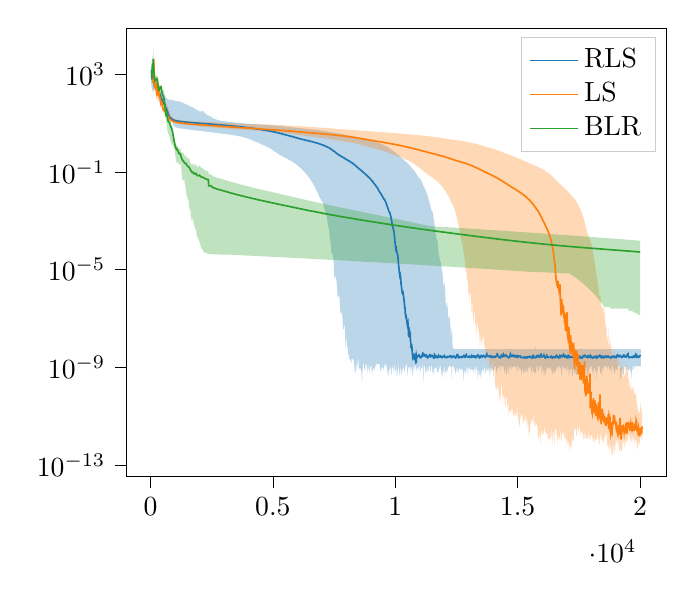
\begin{tikzpicture}

\definecolor{color0}{rgb}{0.12156862745098,0.466666666666667,0.705882352941177}
\definecolor{color1}{rgb}{1,0.498039215686275,0.0549019607843137}
\definecolor{color2}{rgb}{0.172549019607843,0.627450980392157,0.172549019607843}

\begin{axis}[
legend cell align={left},
legend style={fill opacity=0.8, draw opacity=1, text opacity=1, draw=white!80!black},
log basis y={10},
tick align=outside,
tick pos=left,
x grid style={white!69.0196078431373!black},
xmin=-962, xmax=21082,
xtick style={color=black},
y grid style={white!69.0196078431373!black},
ymin=3.47613449829342e-14, ymax=75355.4931331544,
ymode=log,
ytick style={color=black}
]
\path [fill=color0, fill opacity=0.3]
(axis cs:40,3197.84575291474)
--(axis cs:40,474.251985174285)
--(axis cs:47,327.49216250282)
--(axis cs:54,267.902002259074)
--(axis cs:61,252.640415240168)
--(axis cs:68,267.3730049581)
--(axis cs:75,292.709001821389)
--(axis cs:82,208.520071002363)
--(axis cs:89,191.517032090433)
--(axis cs:96,234.377464390945)
--(axis cs:103,195.303246170848)
--(axis cs:110,195.845535205802)
--(axis cs:117,212.961931047489)
--(axis cs:124,233.867463111805)
--(axis cs:131,259.708693590868)
--(axis cs:138,266.565371475291)
--(axis cs:145,351.223990179563)
--(axis cs:152,308.450565154362)
--(axis cs:159,274.123228692813)
--(axis cs:166,241.406392844251)
--(axis cs:173,247.502685697411)
--(axis cs:180,240.972224097889)
--(axis cs:187,241.252512419162)
--(axis cs:194,263.059100724497)
--(axis cs:201,274.231105608732)
--(axis cs:208,285.827719536382)
--(axis cs:215,266.946699426347)
--(axis cs:222,238.751664727275)
--(axis cs:229,233.352416703172)
--(axis cs:236,250.915163197116)
--(axis cs:243,229.702352418377)
--(axis cs:250,207.587164705724)
--(axis cs:257,191.738203333658)
--(axis cs:264,203.25032660778)
--(axis cs:271,206.332794591767)
--(axis cs:278,187.765114304553)
--(axis cs:285,171.249669635219)
--(axis cs:292,147.879811810191)
--(axis cs:299,136.61123618795)
--(axis cs:306,111.874837092634)
--(axis cs:313,116.916562680582)
--(axis cs:320,139.092576892554)
--(axis cs:327,137.508969174069)
--(axis cs:334,137.441942887982)
--(axis cs:341,118.467015636019)
--(axis cs:348,103.715099092385)
--(axis cs:355,96.1563450421138)
--(axis cs:362,99.5570135895158)
--(axis cs:369,86.8282950168353)
--(axis cs:376,69.6057929829036)
--(axis cs:383,52.6241573883658)
--(axis cs:390,49.6173884704069)
--(axis cs:397,66.0891279128078)
--(axis cs:404,70.520052070579)
--(axis cs:411,52.7961003031154)
--(axis cs:418,56.3687516688822)
--(axis cs:425,70.2906395674131)
--(axis cs:432,79.9913995545107)
--(axis cs:439,84.1540151182941)
--(axis cs:446,83.9271969742817)
--(axis cs:453,75.0931147470801)
--(axis cs:460,75.054781015526)
--(axis cs:467,86.0743721556522)
--(axis cs:474,79.8613869356516)
--(axis cs:481,75.8280877431198)
--(axis cs:488,73.155683334311)
--(axis cs:495,67.3252947340455)
--(axis cs:502,61.6628400390898)
--(axis cs:509,60.2476426835533)
--(axis cs:516,58.7580643307297)
--(axis cs:523,58.2687659625474)
--(axis cs:530,61.6120980214662)
--(axis cs:537,59.7941984248963)
--(axis cs:544,58.444524240193)
--(axis cs:551,58.0701442865956)
--(axis cs:558,52.9482751906132)
--(axis cs:565,47.8056123803867)
--(axis cs:572,44.197687862134)
--(axis cs:579,41.6068722514689)
--(axis cs:586,38.6719236287289)
--(axis cs:593,35.9147630991693)
--(axis cs:600,34.5596024226152)
--(axis cs:607,33.4227934075949)
--(axis cs:614,32.2999741581968)
--(axis cs:621,30.8146452408697)
--(axis cs:628,31.3694549781929)
--(axis cs:635,30.6756868500073)
--(axis cs:642,29.4696088924419)
--(axis cs:649,30.0016669717734)
--(axis cs:656,30.4662830665362)
--(axis cs:663,30.0292016303712)
--(axis cs:670,29.7355842516807)
--(axis cs:677,26.0026654991996)
--(axis cs:684,23.6086616150657)
--(axis cs:691,22.5700687865996)
--(axis cs:698,22.4023840031212)
--(axis cs:705,21.2285321115441)
--(axis cs:712,19.7837093834914)
--(axis cs:719,18.4876775853932)
--(axis cs:726,17.4042528557153)
--(axis cs:733,16.6888392793658)
--(axis cs:740,15.9403693883662)
--(axis cs:747,15.4436438406536)
--(axis cs:754,15.1964034294648)
--(axis cs:761,15.0862465641393)
--(axis cs:768,14.7175244789338)
--(axis cs:775,14.4358249229656)
--(axis cs:782,14.2187509355842)
--(axis cs:789,14.1836976099854)
--(axis cs:796,14.2810627857512)
--(axis cs:803,14.2632544165252)
--(axis cs:810,14.2785356329758)
--(axis cs:817,14.2130057886627)
--(axis cs:824,14.0568755150852)
--(axis cs:831,13.9180862527814)
--(axis cs:838,13.8457513613551)
--(axis cs:845,13.8290485209758)
--(axis cs:852,13.1426540631675)
--(axis cs:859,12.9610993376529)
--(axis cs:866,12.2893403778454)
--(axis cs:873,12.1527685649321)
--(axis cs:880,12.664156003567)
--(axis cs:887,12.5432541391011)
--(axis cs:894,11.9707276569342)
--(axis cs:901,10.8967390497469)
--(axis cs:908,10.2575717266813)
--(axis cs:915,10.0208764150583)
--(axis cs:922,9.20165861416571)
--(axis cs:929,8.59908139781128)
--(axis cs:936,8.26192440215103)
--(axis cs:943,7.87458291032281)
--(axis cs:950,7.63750129915846)
--(axis cs:957,7.57017607568961)
--(axis cs:964,7.48719711898767)
--(axis cs:971,7.51117406471678)
--(axis cs:978,7.51344465197001)
--(axis cs:985,7.81257531623869)
--(axis cs:992,7.39153709011538)
--(axis cs:999,7.19063791351213)
--(axis cs:1006,7.0906118783899)
--(axis cs:1013,6.90078198260014)
--(axis cs:1020,6.699669929747)
--(axis cs:1027,6.53637413388748)
--(axis cs:1034,6.4780727656005)
--(axis cs:1041,6.45242597410523)
--(axis cs:1048,6.51049254133887)
--(axis cs:1055,6.56714469753261)
--(axis cs:1062,6.6452424932776)
--(axis cs:1069,6.66529131747153)
--(axis cs:1076,6.55248161354888)
--(axis cs:1083,6.45502583427064)
--(axis cs:1090,6.38876618272452)
--(axis cs:1097,6.34520152377958)
--(axis cs:1104,6.32478619313368)
--(axis cs:1111,6.34671011734728)
--(axis cs:1118,6.33067244937375)
--(axis cs:1125,6.27906207762741)
--(axis cs:1132,6.23985543970617)
--(axis cs:1139,6.2207180144398)
--(axis cs:1146,6.20324781596447)
--(axis cs:1153,6.19297267980265)
--(axis cs:1160,6.18806117753144)
--(axis cs:1167,6.18238198476259)
--(axis cs:1174,6.17221153747569)
--(axis cs:1181,6.16009119592845)
--(axis cs:1188,6.15118710446629)
--(axis cs:1195,6.1292457188496)
--(axis cs:1202,6.11587443149168)
--(axis cs:1209,6.10113196858723)
--(axis cs:1216,6.08889132918291)
--(axis cs:1223,6.07231115124144)
--(axis cs:1230,6.05455645917684)
--(axis cs:1237,6.03430646846394)
--(axis cs:1244,6.01476743377138)
--(axis cs:1251,5.99793795559139)
--(axis cs:1258,5.98141483691399)
--(axis cs:1265,5.96657514494668)
--(axis cs:1272,5.95375920994984)
--(axis cs:1279,5.94115498890639)
--(axis cs:1286,5.92838181031056)
--(axis cs:1293,5.91839871617168)
--(axis cs:1300,5.90763374771133)
--(axis cs:1307,5.90151079416659)
--(axis cs:1314,5.89600148495812)
--(axis cs:1321,5.89653249642387)
--(axis cs:1328,5.90619923840232)
--(axis cs:1335,5.86898377273441)
--(axis cs:1342,5.83953406242032)
--(axis cs:1349,5.81623885047716)
--(axis cs:1356,5.79969132525141)
--(axis cs:1363,5.78625227407138)
--(axis cs:1370,5.77272468847742)
--(axis cs:1377,5.76347743533591)
--(axis cs:1384,5.75398041813649)
--(axis cs:1391,5.7472993417753)
--(axis cs:1398,5.73179206655145)
--(axis cs:1405,5.71876819443449)
--(axis cs:1412,5.7025902495455)
--(axis cs:1419,5.68755083474735)
--(axis cs:1426,5.6744522589146)
--(axis cs:1433,5.66056038050306)
--(axis cs:1440,5.6471236549766)
--(axis cs:1447,5.63610406451008)
--(axis cs:1454,5.62617797416418)
--(axis cs:1461,5.61666098686555)
--(axis cs:1468,5.60312035551908)
--(axis cs:1475,5.58852022117593)
--(axis cs:1482,5.57252349495947)
--(axis cs:1489,5.55751665476559)
--(axis cs:1496,5.54332379617146)
--(axis cs:1503,5.52846415591665)
--(axis cs:1510,5.51317458152398)
--(axis cs:1517,5.50204101824092)
--(axis cs:1524,5.49500516621246)
--(axis cs:1531,5.49295008525815)
--(axis cs:1538,5.48215654362093)
--(axis cs:1545,5.46365904165899)
--(axis cs:1552,5.45425349569148)
--(axis cs:1559,5.43927240245063)
--(axis cs:1566,5.42476209717119)
--(axis cs:1573,5.41113399905217)
--(axis cs:1580,5.39523198889737)
--(axis cs:1587,5.37933011153401)
--(axis cs:1594,5.36464014063624)
--(axis cs:1601,5.34967293759643)
--(axis cs:1608,5.33726851130974)
--(axis cs:1615,5.32502606819169)
--(axis cs:1622,5.31249780273464)
--(axis cs:1629,5.29840250311742)
--(axis cs:1636,5.28598282271027)
--(axis cs:1643,5.27107779466195)
--(axis cs:1650,5.25876663389107)
--(axis cs:1657,5.24975709354213)
--(axis cs:1664,5.23884806044512)
--(axis cs:1671,5.23099537423403)
--(axis cs:1678,5.21781111662555)
--(axis cs:1685,5.20148044417417)
--(axis cs:1692,5.18463082756038)
--(axis cs:1699,5.17144469378024)
--(axis cs:1706,5.16151892500315)
--(axis cs:1713,5.14835759284329)
--(axis cs:1720,5.13782009458705)
--(axis cs:1727,5.13244067664005)
--(axis cs:1734,5.12331046272119)
--(axis cs:1741,5.10896050343873)
--(axis cs:1748,5.09532858269229)
--(axis cs:1755,5.08392278410613)
--(axis cs:1762,5.07213050300737)
--(axis cs:1769,5.06306213015662)
--(axis cs:1776,5.05097795550751)
--(axis cs:1783,5.04098024438571)
--(axis cs:1790,5.03276285389056)
--(axis cs:1797,5.02505528495827)
--(axis cs:1804,5.01286274149624)
--(axis cs:1811,5.00229306456294)
--(axis cs:1818,4.99315738451941)
--(axis cs:1825,4.98564386940645)
--(axis cs:1832,4.97652235745509)
--(axis cs:1839,4.9701578499434)
--(axis cs:1846,4.96451346447951)
--(axis cs:1853,4.95764883354049)
--(axis cs:1860,4.95048367862979)
--(axis cs:1867,4.94415284559773)
--(axis cs:1874,4.93670102569844)
--(axis cs:1881,4.92889601067397)
--(axis cs:1888,4.92012868831819)
--(axis cs:1895,4.90989377408454)
--(axis cs:1902,4.89949238277701)
--(axis cs:1909,4.88959530315007)
--(axis cs:1916,4.87911321041093)
--(axis cs:1923,4.86930320494534)
--(axis cs:1930,4.86100811863989)
--(axis cs:1937,4.8541393182171)
--(axis cs:1944,4.8485692331015)
--(axis cs:1951,4.84464485280616)
--(axis cs:1958,4.84205461755414)
--(axis cs:1965,4.83933884836384)
--(axis cs:1972,4.82958577590354)
--(axis cs:1979,4.81869174766512)
--(axis cs:1986,4.80815680603705)
--(axis cs:1993,4.80003829340959)
--(axis cs:2000,4.7925606393645)
--(axis cs:2007,4.78114450632026)
--(axis cs:2014,4.76852528750301)
--(axis cs:2021,4.75727849985998)
--(axis cs:2028,4.74778237412283)
--(axis cs:2035,4.73884418991603)
--(axis cs:2042,4.73151781642047)
--(axis cs:2049,4.72349135223892)
--(axis cs:2056,4.71534129122565)
--(axis cs:2063,4.70720237158169)
--(axis cs:2070,4.69883322804777)
--(axis cs:2077,4.69038130721654)
--(axis cs:2084,4.68339184320363)
--(axis cs:2091,4.67882271469254)
--(axis cs:2098,4.67580661743237)
--(axis cs:2105,4.67321842312812)
--(axis cs:2112,4.66794732184917)
--(axis cs:2119,4.65650595199475)
--(axis cs:2126,4.64509575739131)
--(axis cs:2133,4.63671064826846)
--(axis cs:2140,4.62900431170194)
--(axis cs:2147,4.62564333840979)
--(axis cs:2154,4.6192813917744)
--(axis cs:2161,4.61092686331909)
--(axis cs:2168,4.60189635470604)
--(axis cs:2175,4.59199276553187)
--(axis cs:2182,4.58333770773985)
--(axis cs:2189,4.57254283532768)
--(axis cs:2196,4.56234142032921)
--(axis cs:2203,4.55289906547419)
--(axis cs:2210,4.5429051755098)
--(axis cs:2217,4.53279342919658)
--(axis cs:2224,4.52425376478263)
--(axis cs:2231,4.51402472965136)
--(axis cs:2238,4.50420506593512)
--(axis cs:2245,4.49553106439889)
--(axis cs:2252,4.48872008095626)
--(axis cs:2259,4.47960779604988)
--(axis cs:2266,4.46955268073958)
--(axis cs:2273,4.46162849545773)
--(axis cs:2280,4.45451711136213)
--(axis cs:2287,4.44566446024868)
--(axis cs:2294,4.43691550031283)
--(axis cs:2301,4.42662479339392)
--(axis cs:2308,4.41649090643694)
--(axis cs:2315,4.40563680509278)
--(axis cs:2322,4.39555516712336)
--(axis cs:2329,4.38627723034438)
--(axis cs:2336,4.38008059425735)
--(axis cs:2343,4.3727905980753)
--(axis cs:2350,4.36132600745856)
--(axis cs:2357,4.34808217196387)
--(axis cs:2364,4.33754827662358)
--(axis cs:2371,4.32761214418332)
--(axis cs:2378,4.31705230545042)
--(axis cs:2385,4.30593205761376)
--(axis cs:2392,4.29549538730888)
--(axis cs:2399,4.28535787524853)
--(axis cs:2406,4.27649724020492)
--(axis cs:2413,4.26933961924469)
--(axis cs:2420,4.25984289537514)
--(axis cs:2427,4.25297342685155)
--(axis cs:2434,4.24550562447242)
--(axis cs:2441,4.23578900150234)
--(axis cs:2448,4.22856373200499)
--(axis cs:2455,4.21881451528271)
--(axis cs:2462,4.21171469992094)
--(axis cs:2469,4.20259795752025)
--(axis cs:2476,4.19094690307713)
--(axis cs:2483,4.18122608946162)
--(axis cs:2490,4.17097406433988)
--(axis cs:2497,4.1589904143264)
--(axis cs:2504,4.14755026069797)
--(axis cs:2511,4.13711411853617)
--(axis cs:2518,4.12832583304699)
--(axis cs:2525,4.1204893369608)
--(axis cs:2532,4.11724460483417)
--(axis cs:2539,4.11369351503219)
--(axis cs:2546,4.10297880922484)
--(axis cs:2553,4.09248129159529)
--(axis cs:2560,4.07838074752494)
--(axis cs:2567,4.06949101853703)
--(axis cs:2574,4.06337054988847)
--(axis cs:2581,4.05134422629331)
--(axis cs:2588,4.04183220084877)
--(axis cs:2595,4.03142769646738)
--(axis cs:2602,4.02184170682386)
--(axis cs:2609,4.01173003857801)
--(axis cs:2616,4.00186811039181)
--(axis cs:2623,3.99381872299942)
--(axis cs:2630,3.98279786759005)
--(axis cs:2637,3.97032301138855)
--(axis cs:2644,3.96038409013969)
--(axis cs:2651,3.94965854757986)
--(axis cs:2658,3.94040829938619)
--(axis cs:2665,3.93334123240412)
--(axis cs:2672,3.92334322250048)
--(axis cs:2679,3.91337784465625)
--(axis cs:2686,3.90436796422407)
--(axis cs:2693,3.89575986842208)
--(axis cs:2700,3.88717610354411)
--(axis cs:2707,3.87912388889832)
--(axis cs:2714,3.87343728158045)
--(axis cs:2721,3.86814511816072)
--(axis cs:2728,3.86354989422301)
--(axis cs:2735,3.86264362104907)
--(axis cs:2742,3.86310088902257)
--(axis cs:2749,3.85747711307143)
--(axis cs:2756,3.8473575894131)
--(axis cs:2763,3.83753017124305)
--(axis cs:2770,3.83113666225051)
--(axis cs:2777,3.82813618024423)
--(axis cs:2784,3.82745765611593)
--(axis cs:2791,3.81648094688407)
--(axis cs:2798,3.80674804433177)
--(axis cs:2805,3.7977030180507)
--(axis cs:2812,3.7902964437429)
--(axis cs:2819,3.78392284989595)
--(axis cs:2826,3.77850622938388)
--(axis cs:2833,3.77066294004969)
--(axis cs:2840,3.7634884633509)
--(axis cs:2847,3.75685387952949)
--(axis cs:2854,3.75078148391934)
--(axis cs:2861,3.74600128803359)
--(axis cs:2868,3.74258321639045)
--(axis cs:2875,3.73468600532263)
--(axis cs:2882,3.72846073491797)
--(axis cs:2889,3.72097613113709)
--(axis cs:2896,3.7133759581405)
--(axis cs:2903,3.70607463693849)
--(axis cs:2910,3.69931667607175)
--(axis cs:2917,3.69284268697053)
--(axis cs:2924,3.68500139068984)
--(axis cs:2931,3.67614974326807)
--(axis cs:2938,3.66813156472201)
--(axis cs:2945,3.66160666961278)
--(axis cs:2952,3.65467377286744)
--(axis cs:2959,3.64827417985078)
--(axis cs:2966,3.64081084828122)
--(axis cs:2973,3.63403165955591)
--(axis cs:2980,3.62870867277687)
--(axis cs:2987,3.62332687427464)
--(axis cs:2994,3.61910003852181)
--(axis cs:3001,3.61649368356082)
--(axis cs:3008,3.62183242618887)
--(axis cs:3015,3.61012614770721)
--(axis cs:3022,3.60221559991697)
--(axis cs:3029,3.59627095957178)
--(axis cs:3036,3.58960269249539)
--(axis cs:3043,3.58205151525595)
--(axis cs:3050,3.57345944375976)
--(axis cs:3057,3.56562094451453)
--(axis cs:3064,3.55747098928527)
--(axis cs:3071,3.54956070423742)
--(axis cs:3078,3.54197858611152)
--(axis cs:3085,3.53651686251623)
--(axis cs:3092,3.52751734062904)
--(axis cs:3099,3.51796417056803)
--(axis cs:3106,3.50818781583575)
--(axis cs:3113,3.49842961569722)
--(axis cs:3120,3.48874382032437)
--(axis cs:3127,3.48072458723894)
--(axis cs:3134,3.47267224781024)
--(axis cs:3141,3.46501819463868)
--(axis cs:3148,3.45712914228841)
--(axis cs:3155,3.44776296331559)
--(axis cs:3162,3.43901811867185)
--(axis cs:3169,3.4309366749207)
--(axis cs:3176,3.422633972878)
--(axis cs:3183,3.41459093697653)
--(axis cs:3190,3.40721532674506)
--(axis cs:3197,3.40305813964871)
--(axis cs:3204,3.39742084160732)
--(axis cs:3211,3.3897026391705)
--(axis cs:3218,3.38248397984706)
--(axis cs:3225,3.3739635237078)
--(axis cs:3232,3.36737014970629)
--(axis cs:3239,3.36258856436129)
--(axis cs:3246,3.35658065946193)
--(axis cs:3253,3.34914952140308)
--(axis cs:3260,3.34343199477037)
--(axis cs:3267,3.33657762522698)
--(axis cs:3274,3.32707184382277)
--(axis cs:3281,3.31738126654352)
--(axis cs:3288,3.30757148127316)
--(axis cs:3295,3.29964550938021)
--(axis cs:3302,3.29127169773536)
--(axis cs:3309,3.28336719584072)
--(axis cs:3316,3.27554323463586)
--(axis cs:3323,3.26761260211742)
--(axis cs:3330,3.25901646722738)
--(axis cs:3337,3.25110855125701)
--(axis cs:3344,3.2421802961059)
--(axis cs:3351,3.23382575782432)
--(axis cs:3358,3.22450025670735)
--(axis cs:3365,3.21573043284107)
--(axis cs:3372,3.20649780860633)
--(axis cs:3379,3.19770561672656)
--(axis cs:3386,3.19040562441652)
--(axis cs:3393,3.18543480245892)
--(axis cs:3400,3.18259105042384)
--(axis cs:3407,3.17969293690858)
--(axis cs:3414,3.16772213610086)
--(axis cs:3421,3.15576190087818)
--(axis cs:3428,3.14449166112585)
--(axis cs:3435,3.13656796501648)
--(axis cs:3442,3.12717932331298)
--(axis cs:3449,3.11799692104513)
--(axis cs:3456,3.10955486092358)
--(axis cs:3463,3.10090990588458)
--(axis cs:3470,3.09175613219888)
--(axis cs:3477,3.08335835871767)
--(axis cs:3484,3.07414292599307)
--(axis cs:3491,3.06424478619487)
--(axis cs:3498,3.05435351616446)
--(axis cs:3505,3.04619574192143)
--(axis cs:3512,3.03859092602884)
--(axis cs:3519,3.03316501134073)
--(axis cs:3526,3.02253661528246)
--(axis cs:3533,3.0133952786682)
--(axis cs:3540,3.00261226300984)
--(axis cs:3547,2.99145431825311)
--(axis cs:3554,2.97996079411016)
--(axis cs:3561,2.96841122906026)
--(axis cs:3568,2.95765848539497)
--(axis cs:3575,2.9477769076662)
--(axis cs:3582,2.93793431067245)
--(axis cs:3589,2.92826829954951)
--(axis cs:3596,2.91852440612459)
--(axis cs:3603,2.90914434909178)
--(axis cs:3610,2.89877946952314)
--(axis cs:3617,2.88922519875237)
--(axis cs:3624,2.88054279249269)
--(axis cs:3631,2.87512567435643)
--(axis cs:3638,2.86884001260847)
--(axis cs:3645,2.85849097350363)
--(axis cs:3652,2.84812607222821)
--(axis cs:3659,2.83982692665608)
--(axis cs:3666,2.83021963078639)
--(axis cs:3673,2.8187581085479)
--(axis cs:3680,2.80889806456797)
--(axis cs:3687,2.79929921322206)
--(axis cs:3694,2.79090766975681)
--(axis cs:3701,2.77940086352937)
--(axis cs:3708,2.76607436038365)
--(axis cs:3715,2.75431154454009)
--(axis cs:3722,2.74410266421972)
--(axis cs:3729,2.73225120334843)
--(axis cs:3736,2.72216071371241)
--(axis cs:3743,2.70933853417244)
--(axis cs:3750,2.69651240716917)
--(axis cs:3757,2.68232603091988)
--(axis cs:3764,2.66946359083771)
--(axis cs:3771,2.65740468120789)
--(axis cs:3778,2.64629785576949)
--(axis cs:3785,2.6363044973467)
--(axis cs:3792,2.62835805834059)
--(axis cs:3799,2.62562938072718)
--(axis cs:3806,2.61654942518028)
--(axis cs:3813,2.60853107214212)
--(axis cs:3820,2.59701193791179)
--(axis cs:3827,2.58276979926403)
--(axis cs:3834,2.56858088664878)
--(axis cs:3841,2.55380321957747)
--(axis cs:3848,2.54146288865103)
--(axis cs:3855,2.52863932138008)
--(axis cs:3862,2.51718134584808)
--(axis cs:3869,2.50900560771048)
--(axis cs:3876,2.50299570448116)
--(axis cs:3883,2.48865685715194)
--(axis cs:3890,2.47704536498559)
--(axis cs:3897,2.46396344437238)
--(axis cs:3904,2.45322208356927)
--(axis cs:3911,2.44085140275314)
--(axis cs:3918,2.42848375311525)
--(axis cs:3925,2.4157820592968)
--(axis cs:3932,2.40420602430563)
--(axis cs:3939,2.39298236485894)
--(axis cs:3946,2.38220481167121)
--(axis cs:3953,2.36980017641423)
--(axis cs:3960,2.35791399376371)
--(axis cs:3967,2.3477996816189)
--(axis cs:3974,2.33544938717609)
--(axis cs:3981,2.32433930942152)
--(axis cs:3988,2.31514084560462)
--(axis cs:3995,2.30570764583011)
--(axis cs:4002,2.29826366042652)
--(axis cs:4009,2.28171173748177)
--(axis cs:4016,2.26606109404753)
--(axis cs:4023,2.24966116202743)
--(axis cs:4030,2.23383535376362)
--(axis cs:4037,2.21921585146303)
--(axis cs:4044,2.20422596456206)
--(axis cs:4051,2.18878599756576)
--(axis cs:4058,2.17387340084733)
--(axis cs:4065,2.15986726736033)
--(axis cs:4072,2.14392850801121)
--(axis cs:4079,2.12856048528117)
--(axis cs:4086,2.11278423714564)
--(axis cs:4093,2.0958759156615)
--(axis cs:4100,2.08068031041564)
--(axis cs:4107,2.07188310183301)
--(axis cs:4114,2.06339060102844)
--(axis cs:4121,2.05364085820037)
--(axis cs:4128,2.03331725513254)
--(axis cs:4135,2.01664428835776)
--(axis cs:4142,2.0032467027461)
--(axis cs:4149,1.99112099288471)
--(axis cs:4156,1.97758591775214)
--(axis cs:4163,1.96801195746668)
--(axis cs:4170,1.95737644399225)
--(axis cs:4177,1.95086168574747)
--(axis cs:4184,1.93601308138259)
--(axis cs:4191,1.91894049045344)
--(axis cs:4198,1.90326120469646)
--(axis cs:4205,1.88478389857877)
--(axis cs:4212,1.8674450762559)
--(axis cs:4219,1.85232244222401)
--(axis cs:4226,1.84021232872654)
--(axis cs:4233,1.8272093567889)
--(axis cs:4240,1.81376401799356)
--(axis cs:4247,1.80012029913413)
--(axis cs:4254,1.78634415451006)
--(axis cs:4261,1.77239541861298)
--(axis cs:4268,1.75843897433587)
--(axis cs:4275,1.74744632850798)
--(axis cs:4282,1.7403264711005)
--(axis cs:4289,1.73314377647642)
--(axis cs:4296,1.71954158456252)
--(axis cs:4303,1.7070844362896)
--(axis cs:4310,1.6941190683806)
--(axis cs:4317,1.68233086547238)
--(axis cs:4324,1.67240445751185)
--(axis cs:4331,1.66385040603172)
--(axis cs:4338,1.65088404177682)
--(axis cs:4345,1.63912009785182)
--(axis cs:4352,1.63662400764743)
--(axis cs:4359,1.63610742777587)
--(axis cs:4366,1.64003800416902)
--(axis cs:4373,1.62275339144831)
--(axis cs:4380,1.60861236811787)
--(axis cs:4387,1.59035575478777)
--(axis cs:4394,1.57697989675935)
--(axis cs:4401,1.56597892048232)
--(axis cs:4408,1.55656431361081)
--(axis cs:4415,1.5472997198578)
--(axis cs:4422,1.53890549948179)
--(axis cs:4429,1.53154885501943)
--(axis cs:4436,1.51874893585034)
--(axis cs:4443,1.50697341292253)
--(axis cs:4450,1.49604325877747)
--(axis cs:4457,1.48205838490061)
--(axis cs:4464,1.46662464774417)
--(axis cs:4471,1.45309652227317)
--(axis cs:4478,1.43973443801523)
--(axis cs:4485,1.4294810471033)
--(axis cs:4492,1.42128618081014)
--(axis cs:4499,1.41409878370921)
--(axis cs:4506,1.40938706001126)
--(axis cs:4513,1.40005420599595)
--(axis cs:4520,1.39061008387369)
--(axis cs:4527,1.37799657880657)
--(axis cs:4534,1.36600745371836)
--(axis cs:4541,1.35507274766111)
--(axis cs:4548,1.34425272015204)
--(axis cs:4555,1.33067691867689)
--(axis cs:4562,1.31697639584761)
--(axis cs:4569,1.30554006111319)
--(axis cs:4576,1.29347482783479)
--(axis cs:4583,1.28231254954861)
--(axis cs:4590,1.2729209437121)
--(axis cs:4597,1.2647529541162)
--(axis cs:4604,1.25454065362396)
--(axis cs:4611,1.24597711158287)
--(axis cs:4618,1.23543872627825)
--(axis cs:4625,1.22752755966924)
--(axis cs:4632,1.21927579897107)
--(axis cs:4639,1.21576046490462)
--(axis cs:4646,1.20620964666678)
--(axis cs:4653,1.20076373521562)
--(axis cs:4660,1.19457961010571)
--(axis cs:4667,1.18726352815358)
--(axis cs:4674,1.18138217912589)
--(axis cs:4681,1.17464729553907)
--(axis cs:4688,1.17951433050183)
--(axis cs:4695,1.15946812587261)
--(axis cs:4702,1.14905713814699)
--(axis cs:4709,1.13851554952929)
--(axis cs:4716,1.12744316108736)
--(axis cs:4723,1.11723621478486)
--(axis cs:4730,1.10806461335301)
--(axis cs:4737,1.10036297674603)
--(axis cs:4744,1.09058983735734)
--(axis cs:4751,1.08364920938448)
--(axis cs:4758,1.07553496474212)
--(axis cs:4765,1.06802087065272)
--(axis cs:4772,1.05748809785354)
--(axis cs:4779,1.04403261584802)
--(axis cs:4786,1.03285414393169)
--(axis cs:4793,1.02598114445374)
--(axis cs:4800,1.01990204158574)
--(axis cs:4807,1.01402723080659)
--(axis cs:4814,1.01037700749252)
--(axis cs:4821,1.00018204680161)
--(axis cs:4828,0.98969198735601)
--(axis cs:4835,0.979609882122265)
--(axis cs:4842,0.968014992972451)
--(axis cs:4849,0.957152127012316)
--(axis cs:4856,0.947801080322697)
--(axis cs:4863,0.939879585192971)
--(axis cs:4870,0.932225109818701)
--(axis cs:4877,0.925330887560397)
--(axis cs:4884,0.920130552369809)
--(axis cs:4891,0.909365975278469)
--(axis cs:4898,0.899218036329549)
--(axis cs:4905,0.888135435274824)
--(axis cs:4912,0.877622084919459)
--(axis cs:4919,0.867648318753561)
--(axis cs:4926,0.860407861401942)
--(axis cs:4933,0.851099427319572)
--(axis cs:4940,0.842568692322392)
--(axis cs:4947,0.834182698361099)
--(axis cs:4954,0.824437222674524)
--(axis cs:4961,0.814497686179758)
--(axis cs:4968,0.804494353228631)
--(axis cs:4975,0.796068260859711)
--(axis cs:4982,0.786972585386766)
--(axis cs:4989,0.778567860814908)
--(axis cs:4996,0.770342942319447)
--(axis cs:5003,0.764341420963645)
--(axis cs:5010,0.759044464847628)
--(axis cs:5017,0.752159654913816)
--(axis cs:5024,0.745530165699128)
--(axis cs:5031,0.736974672288724)
--(axis cs:5038,0.725641592171745)
--(axis cs:5045,0.714598359313217)
--(axis cs:5052,0.706139075816162)
--(axis cs:5059,0.698197797737825)
--(axis cs:5066,0.690230411842109)
--(axis cs:5073,0.681521816828187)
--(axis cs:5080,0.675693586338916)
--(axis cs:5087,0.670546515605364)
--(axis cs:5094,0.664624974663453)
--(axis cs:5101,0.659747601651055)
--(axis cs:5108,0.654945639021555)
--(axis cs:5115,0.650988434162296)
--(axis cs:5122,0.642721633655256)
--(axis cs:5129,0.634785680867453)
--(axis cs:5136,0.62715391190496)
--(axis cs:5143,0.618685896518885)
--(axis cs:5150,0.611587484881541)
--(axis cs:5157,0.605721324438704)
--(axis cs:5164,0.598987930805139)
--(axis cs:5171,0.592548209797104)
--(axis cs:5178,0.585144469142586)
--(axis cs:5185,0.579339300322972)
--(axis cs:5192,0.572419824911742)
--(axis cs:5199,0.567134202567698)
--(axis cs:5206,0.562063455001072)
--(axis cs:5213,0.556379027282922)
--(axis cs:5220,0.550599704330012)
--(axis cs:5227,0.545195089259688)
--(axis cs:5234,0.540702767082882)
--(axis cs:5241,0.536353213919725)
--(axis cs:5248,0.530644075308558)
--(axis cs:5255,0.524997741622442)
--(axis cs:5262,0.519886153665247)
--(axis cs:5269,0.514860006973708)
--(axis cs:5276,0.50820141947941)
--(axis cs:5283,0.501861766487993)
--(axis cs:5290,0.49626778706432)
--(axis cs:5297,0.490743532803994)
--(axis cs:5304,0.485664082160019)
--(axis cs:5311,0.480798650185965)
--(axis cs:5318,0.475873561419161)
--(axis cs:5325,0.471318002859241)
--(axis cs:5332,0.466590236353589)
--(axis cs:5339,0.462666688961473)
--(axis cs:5346,0.45894453768168)
--(axis cs:5353,0.455225166518501)
--(axis cs:5360,0.451892613539229)
--(axis cs:5367,0.448954514438433)
--(axis cs:5374,0.44498635677792)
--(axis cs:5381,0.439878774229717)
--(axis cs:5388,0.436004959743309)
--(axis cs:5395,0.433900375157426)
--(axis cs:5402,0.430453291228153)
--(axis cs:5409,0.427117789891636)
--(axis cs:5416,0.423396723492654)
--(axis cs:5423,0.419842048455033)
--(axis cs:5430,0.416114596079474)
--(axis cs:5437,0.412648493981561)
--(axis cs:5444,0.409210805694373)
--(axis cs:5451,0.405088362405356)
--(axis cs:5458,0.401177048416888)
--(axis cs:5465,0.396973881624983)
--(axis cs:5472,0.393351859223313)
--(axis cs:5479,0.389887972764953)
--(axis cs:5486,0.387418765252674)
--(axis cs:5493,0.385415945782198)
--(axis cs:5500,0.381955191923597)
--(axis cs:5507,0.377995939259833)
--(axis cs:5514,0.374662346740875)
--(axis cs:5521,0.371142612878277)
--(axis cs:5528,0.368005736766934)
--(axis cs:5535,0.3656448188555)
--(axis cs:5542,0.362799554506139)
--(axis cs:5549,0.361076374349011)
--(axis cs:5556,0.358360555684121)
--(axis cs:5563,0.355985473333805)
--(axis cs:5570,0.353182059731882)
--(axis cs:5577,0.34987742116601)
--(axis cs:5584,0.346615887928037)
--(axis cs:5591,0.343289909011217)
--(axis cs:5598,0.340367369275847)
--(axis cs:5605,0.336866815013251)
--(axis cs:5612,0.333842324609554)
--(axis cs:5619,0.330165623030765)
--(axis cs:5626,0.326605088887164)
--(axis cs:5633,0.323024746003599)
--(axis cs:5640,0.319300953541672)
--(axis cs:5647,0.316242547963248)
--(axis cs:5654,0.312869662374741)
--(axis cs:5661,0.309680078863338)
--(axis cs:5668,0.306682306236509)
--(axis cs:5675,0.304110294142714)
--(axis cs:5682,0.301653460748016)
--(axis cs:5689,0.299821025939859)
--(axis cs:5696,0.297437054241001)
--(axis cs:5703,0.294167752626578)
--(axis cs:5710,0.292171870980626)
--(axis cs:5717,0.289354464148153)
--(axis cs:5724,0.28683516597074)
--(axis cs:5731,0.284720437311637)
--(axis cs:5738,0.283525897019812)
--(axis cs:5745,0.2820823736335)
--(axis cs:5752,0.280448072818671)
--(axis cs:5759,0.279353540382865)
--(axis cs:5766,0.277204443490822)
--(axis cs:5773,0.274364205348608)
--(axis cs:5780,0.271176559466656)
--(axis cs:5787,0.267238600146346)
--(axis cs:5794,0.263349592184382)
--(axis cs:5801,0.260314582671314)
--(axis cs:5808,0.258348176057989)
--(axis cs:5815,0.255672679371272)
--(axis cs:5822,0.252002428441251)
--(axis cs:5829,0.248456349484494)
--(axis cs:5836,0.244702577724433)
--(axis cs:5843,0.240837944072278)
--(axis cs:5850,0.237256554160779)
--(axis cs:5857,0.233949421623202)
--(axis cs:5864,0.230655458406396)
--(axis cs:5871,0.227689788172961)
--(axis cs:5878,0.225307485625521)
--(axis cs:5885,0.223180236075752)
--(axis cs:5892,0.22168719125724)
--(axis cs:5899,0.220143580772269)
--(axis cs:5906,0.218008123459319)
--(axis cs:5913,0.215816073906369)
--(axis cs:5920,0.21368664006818)
--(axis cs:5927,0.211644498061866)
--(axis cs:5934,0.209887827176104)
--(axis cs:5941,0.208234151852728)
--(axis cs:5948,0.206718797815386)
--(axis cs:5955,0.204432420057539)
--(axis cs:5962,0.201716876532118)
--(axis cs:5969,0.198728792706942)
--(axis cs:5976,0.19591703147046)
--(axis cs:5983,0.193140001831923)
--(axis cs:5990,0.190535400936567)
--(axis cs:5997,0.188108785355811)
--(axis cs:6004,0.185272220657753)
--(axis cs:6011,0.182835909924731)
--(axis cs:6018,0.180518070355502)
--(axis cs:6025,0.178294253562092)
--(axis cs:6032,0.176135761566103)
--(axis cs:6039,0.173851231180281)
--(axis cs:6046,0.171039870336289)
--(axis cs:6053,0.168474258664594)
--(axis cs:6060,0.165843911969182)
--(axis cs:6067,0.163585932468966)
--(axis cs:6074,0.161375426931714)
--(axis cs:6081,0.159289432676962)
--(axis cs:6088,0.157033085858913)
--(axis cs:6095,0.154838619841626)
--(axis cs:6102,0.15233884102233)
--(axis cs:6109,0.149831457595831)
--(axis cs:6116,0.148512420555706)
--(axis cs:6123,0.145809062043632)
--(axis cs:6130,0.14349028419129)
--(axis cs:6137,0.141215976126614)
--(axis cs:6144,0.139169196436932)
--(axis cs:6151,0.137786734216851)
--(axis cs:6158,0.1365345289196)
--(axis cs:6165,0.134404864429665)
--(axis cs:6172,0.132006920243862)
--(axis cs:6179,0.13039463306471)
--(axis cs:6186,0.129750762052293)
--(axis cs:6193,0.128931112869115)
--(axis cs:6200,0.12521537692167)
--(axis cs:6207,0.122330451640601)
--(axis cs:6214,0.119989082206756)
--(axis cs:6221,0.117579606416098)
--(axis cs:6228,0.115536827296578)
--(axis cs:6235,0.113425028979561)
--(axis cs:6242,0.110923805983649)
--(axis cs:6249,0.108601893865446)
--(axis cs:6256,0.106600772971462)
--(axis cs:6263,0.104721429451392)
--(axis cs:6270,0.103306826357544)
--(axis cs:6277,0.101871745643879)
--(axis cs:6284,0.100473774951208)
--(axis cs:6291,0.0983349578978829)
--(axis cs:6298,0.0961882237479887)
--(axis cs:6305,0.0943983193372633)
--(axis cs:6312,0.0928941073168241)
--(axis cs:6319,0.0913347395676503)
--(axis cs:6326,0.0898007015295538)
--(axis cs:6333,0.088468316138614)
--(axis cs:6340,0.0869932936997096)
--(axis cs:6347,0.0855425379366082)
--(axis cs:6354,0.0843426340910681)
--(axis cs:6361,0.0832490192240824)
--(axis cs:6368,0.0828260329204228)
--(axis cs:6375,0.0810629345325229)
--(axis cs:6382,0.079181173752105)
--(axis cs:6389,0.0772602492428975)
--(axis cs:6396,0.0753173996572411)
--(axis cs:6403,0.0737596970519397)
--(axis cs:6410,0.0723017542004182)
--(axis cs:6417,0.070026436368403)
--(axis cs:6424,0.0680872718143612)
--(axis cs:6431,0.0667945240947741)
--(axis cs:6438,0.0651250261394369)
--(axis cs:6445,0.0639163889895563)
--(axis cs:6452,0.0625579666003982)
--(axis cs:6459,0.0607905951756558)
--(axis cs:6466,0.0594407105941021)
--(axis cs:6473,0.0577531348287908)
--(axis cs:6480,0.0566592343968722)
--(axis cs:6487,0.0567411915082447)
--(axis cs:6494,0.056944977810894)
--(axis cs:6501,0.0543292194668781)
--(axis cs:6508,0.0528784939626687)
--(axis cs:6515,0.0524348317641648)
--(axis cs:6522,0.0518227807585436)
--(axis cs:6529,0.0505170375367537)
--(axis cs:6536,0.0489595022499712)
--(axis cs:6543,0.0473779290050849)
--(axis cs:6550,0.0459087863494126)
--(axis cs:6557,0.0446742565391589)
--(axis cs:6564,0.04341733263247)
--(axis cs:6571,0.0423333962882817)
--(axis cs:6578,0.0414492464794534)
--(axis cs:6585,0.0408369645130299)
--(axis cs:6592,0.0401833469876591)
--(axis cs:6599,0.0394031836781931)
--(axis cs:6606,0.0383840944833503)
--(axis cs:6613,0.0372208302692687)
--(axis cs:6620,0.0362523609735773)
--(axis cs:6627,0.0352072637723817)
--(axis cs:6634,0.0339376006422166)
--(axis cs:6641,0.0333383487031009)
--(axis cs:6648,0.0321313068037419)
--(axis cs:6655,0.0309919012346023)
--(axis cs:6662,0.0301104943517165)
--(axis cs:6669,0.0289853270515861)
--(axis cs:6676,0.0279410440487508)
--(axis cs:6683,0.0270344250034824)
--(axis cs:6690,0.026315284140379)
--(axis cs:6697,0.0257632741755793)
--(axis cs:6704,0.0254628745804743)
--(axis cs:6711,0.0246692382800935)
--(axis cs:6718,0.0236466848818098)
--(axis cs:6725,0.0225869660373684)
--(axis cs:6732,0.0222043109090113)
--(axis cs:6739,0.0216190563391983)
--(axis cs:6746,0.0207795558548492)
--(axis cs:6753,0.0199016546317849)
--(axis cs:6760,0.0193052760918071)
--(axis cs:6767,0.0186506582025877)
--(axis cs:6774,0.0180748328729156)
--(axis cs:6781,0.0176318644284107)
--(axis cs:6788,0.0171950036012479)
--(axis cs:6795,0.0166196809258762)
--(axis cs:6802,0.0160735765141289)
--(axis cs:6809,0.0156282956607952)
--(axis cs:6816,0.015136392096159)
--(axis cs:6823,0.014756065082398)
--(axis cs:6830,0.0143106048317264)
--(axis cs:6837,0.0138378697783176)
--(axis cs:6844,0.0133429575744148)
--(axis cs:6851,0.0128402989745988)
--(axis cs:6858,0.0123986539107327)
--(axis cs:6865,0.0119421962813463)
--(axis cs:6872,0.0114773680104429)
--(axis cs:6879,0.0110226937872639)
--(axis cs:6886,0.0105974419520307)
--(axis cs:6893,0.0102276392578018)
--(axis cs:6900,0.00984559922121742)
--(axis cs:6907,0.00950811133877692)
--(axis cs:6914,0.00926673134494739)
--(axis cs:6921,0.00903297512225662)
--(axis cs:6928,0.0088531388013967)
--(axis cs:6935,0.00856401691236734)
--(axis cs:6942,0.00834052815706497)
--(axis cs:6949,0.00801056479570884)
--(axis cs:6956,0.007726183973688)
--(axis cs:6963,0.00747054302650829)
--(axis cs:6970,0.00727764661735646)
--(axis cs:6977,0.00704931460243586)
--(axis cs:6984,0.00677715116586462)
--(axis cs:6991,0.00658011306955696)
--(axis cs:6998,0.00645163747112557)
--(axis cs:7005,0.00625961128822035)
--(axis cs:7012,0.00604413533645301)
--(axis cs:7019,0.0058596675021851)
--(axis cs:7026,0.0057276291636097)
--(axis cs:7033,0.00551779621974935)
--(axis cs:7040,0.00530759812932267)
--(axis cs:7047,0.00510459605612193)
--(axis cs:7054,0.00485426223419443)
--(axis cs:7061,0.0046338442974272)
--(axis cs:7068,0.00443784166410413)
--(axis cs:7075,0.00427769186900894)
--(axis cs:7082,0.00401526101695334)
--(axis cs:7089,0.00376309930970166)
--(axis cs:7096,0.00352651967047071)
--(axis cs:7103,0.00329249019421806)
--(axis cs:7110,0.00307581560236468)
--(axis cs:7117,0.00289242842142513)
--(axis cs:7124,0.00273606551350635)
--(axis cs:7131,0.00259070011054418)
--(axis cs:7138,0.00243660705578153)
--(axis cs:7145,0.00232906105902876)
--(axis cs:7152,0.00221863659020535)
--(axis cs:7159,0.00210713532762061)
--(axis cs:7166,0.0020301757332608)
--(axis cs:7173,0.00198739737353102)
--(axis cs:7180,0.00193994781429084)
--(axis cs:7187,0.00182114544691526)
--(axis cs:7194,0.00163779806980113)
--(axis cs:7201,0.00147282000820797)
--(axis cs:7208,0.00134699393119739)
--(axis cs:7215,0.00119839777899875)
--(axis cs:7222,0.00105173408047883)
--(axis cs:7229,0.000904942791476233)
--(axis cs:7236,0.000821333992015441)
--(axis cs:7243,0.00073046725490338)
--(axis cs:7250,0.000707554461003236)
--(axis cs:7257,0.000629306902733824)
--(axis cs:7264,0.000583191857418533)
--(axis cs:7271,0.000553979574526657)
--(axis cs:7278,0.000521220469418717)
--(axis cs:7285,0.000494294864198717)
--(axis cs:7292,0.000464154381884182)
--(axis cs:7299,0.000407087388576797)
--(axis cs:7306,0.000378893784835126)
--(axis cs:7313,0.000289665440527765)
--(axis cs:7320,0.000234757900359669)
--(axis cs:7327,0.000195510866837892)
--(axis cs:7334,0.00017001383446795)
--(axis cs:7341,0.00015769925452427)
--(axis cs:7348,0.000139872304394164)
--(axis cs:7355,0.000129954769204809)
--(axis cs:7362,0.000126553376852178)
--(axis cs:7369,0.000104792633896657)
--(axis cs:7376,8.53315543733558e-05)
--(axis cs:7383,6.09634505416432e-05)
--(axis cs:7390,4.88505734504284e-05)
--(axis cs:7397,4.35930501982026e-05)
--(axis cs:7404,4.72239860664764e-05)
--(axis cs:7411,5.15442985891648e-05)
--(axis cs:7418,5.86155698355232e-05)
--(axis cs:7425,5.04608599926399e-05)
--(axis cs:7432,4.84190083989689e-05)
--(axis cs:7439,4.67694169708359e-05)
--(axis cs:7446,4.06928540957032e-05)
--(axis cs:7453,3.43307302517373e-05)
--(axis cs:7460,3.23456784725056e-05)
--(axis cs:7467,3.13764370216243e-05)
--(axis cs:7474,2.71371411962625e-05)
--(axis cs:7481,2.18843700548362e-05)
--(axis cs:7488,1.62581380797061e-05)
--(axis cs:7495,1.09154650872549e-05)
--(axis cs:7502,7.74908344062447e-06)
--(axis cs:7509,5.41213296342983e-06)
--(axis cs:7516,4.66623141803698e-06)
--(axis cs:7523,4.73181049026386e-06)
--(axis cs:7530,5.39473117983569e-06)
--(axis cs:7537,6.29472487313823e-06)
--(axis cs:7544,5.61856010004621e-06)
--(axis cs:7551,5.07502611662172e-06)
--(axis cs:7558,4.73348386755417e-06)
--(axis cs:7565,4.6346221724791e-06)
--(axis cs:7572,5.00205264856865e-06)
--(axis cs:7579,5.47571027029044e-06)
--(axis cs:7586,4.6096477093719e-06)
--(axis cs:7593,4.00436532410671e-06)
--(axis cs:7600,3.4990190531258e-06)
--(axis cs:7607,3.1128918104182e-06)
--(axis cs:7614,2.18576836309541e-06)
--(axis cs:7621,1.93021765831778e-06)
--(axis cs:7628,1.52742843322217e-06)
--(axis cs:7635,1.3283643801627e-06)
--(axis cs:7642,8.25734447820937e-07)
--(axis cs:7649,7.78967419216676e-07)
--(axis cs:7656,1.01235766503697e-06)
--(axis cs:7663,8.08358455417695e-07)
--(axis cs:7670,7.67356382309687e-07)
--(axis cs:7677,7.76008073893646e-07)
--(axis cs:7684,8.13831470914862e-07)
--(axis cs:7691,8.70181313978022e-07)
--(axis cs:7698,9.24750945516407e-07)
--(axis cs:7705,8.05050118477825e-07)
--(axis cs:7712,7.95627062432668e-07)
--(axis cs:7719,7.35535244167929e-07)
--(axis cs:7726,6.45244806063379e-07)
--(axis cs:7733,4.79460325673237e-07)
--(axis cs:7740,3.23744485808445e-07)
--(axis cs:7747,2.34736668378762e-07)
--(axis cs:7754,2.41339158867397e-07)
--(axis cs:7761,1.78596390310605e-07)
--(axis cs:7768,1.49195676642538e-07)
--(axis cs:7775,1.78007799944785e-07)
--(axis cs:7782,1.8740291507954e-07)
--(axis cs:7789,1.40563820696878e-07)
--(axis cs:7796,1.48319277206317e-07)
--(axis cs:7803,1.7830009840797e-07)
--(axis cs:7810,2.08517175142422e-07)
--(axis cs:7817,2.02369327310706e-07)
--(axis cs:7824,1.81676670624351e-07)
--(axis cs:7831,1.62264705258057e-07)
--(axis cs:7838,1.21414793517114e-07)
--(axis cs:7845,1.00940213504229e-07)
--(axis cs:7852,7.00905495158796e-08)
--(axis cs:7859,5.58666870605895e-08)
--(axis cs:7866,4.36497541072701e-08)
--(axis cs:7873,3.89804474098153e-08)
--(axis cs:7880,3.74635681155655e-08)
--(axis cs:7887,4.08799347316539e-08)
--(axis cs:7894,3.61170532388863e-08)
--(axis cs:7901,3.8902058829335e-08)
--(axis cs:7908,5.62459545628793e-08)
--(axis cs:7915,6.43098681681077e-08)
--(axis cs:7922,5.53045036999068e-08)
--(axis cs:7929,5.18158297371257e-08)
--(axis cs:7936,4.07851421411106e-08)
--(axis cs:7943,3.50440413019227e-08)
--(axis cs:7950,2.40692330989086e-08)
--(axis cs:7957,1.56902350950921e-08)
--(axis cs:7964,9.2657936358832e-09)
--(axis cs:7971,5.51118877770945e-09)
--(axis cs:7978,8.96159184477222e-09)
--(axis cs:7985,1.35118875056459e-08)
--(axis cs:7992,1.77705108617665e-08)
--(axis cs:7999,1.85115186043424e-08)
--(axis cs:8006,1.40867438321159e-08)
--(axis cs:8013,1.11857921045871e-08)
--(axis cs:8020,9.76506419261663e-09)
--(axis cs:8027,7.95088094395501e-09)
--(axis cs:8034,8.44434855128687e-09)
--(axis cs:8041,7.01345674949711e-09)
--(axis cs:8048,7.22967747292755e-09)
--(axis cs:8055,6.26577618948637e-09)
--(axis cs:8062,5.20825957228266e-09)
--(axis cs:8069,4.45668026069227e-09)
--(axis cs:8076,3.26001163609381e-09)
--(axis cs:8083,3.65422528236596e-09)
--(axis cs:8090,4.58203026021766e-09)
--(axis cs:8097,3.48245856333309e-09)
--(axis cs:8104,2.76804884968656e-09)
--(axis cs:8111,2.92438350905309e-09)
--(axis cs:8118,2.39934315719893e-09)
--(axis cs:8125,2.2777696100307e-09)
--(axis cs:8132,2.25626641323892e-09)
--(axis cs:8139,2.8970463189968e-09)
--(axis cs:8146,2.58084754093595e-09)
--(axis cs:8153,2.15282283695496e-09)
--(axis cs:8160,2.07821416807553e-09)
--(axis cs:8167,1.87077857480223e-09)
--(axis cs:8174,1.8713261147804e-09)
--(axis cs:8181,1.94788450058881e-09)
--(axis cs:8188,2.32668016506648e-09)
--(axis cs:8195,2.31561750752972e-09)
--(axis cs:8202,2.23809782702939e-09)
--(axis cs:8209,1.65141497638279e-09)
--(axis cs:8216,1.51275778747144e-09)
--(axis cs:8223,1.63025211869837e-09)
--(axis cs:8230,2.11088988250843e-09)
--(axis cs:8237,2.7139880674543e-09)
--(axis cs:8244,2.61730341042914e-09)
--(axis cs:8251,2.19785256149149e-09)
--(axis cs:8258,2.43216336815601e-09)
--(axis cs:8265,2.56707900570769e-09)
--(axis cs:8272,2.15154687489205e-09)
--(axis cs:8279,2.10201547346331e-09)
--(axis cs:8286,2.20832408779826e-09)
--(axis cs:8293,2.05539458557776e-09)
--(axis cs:8300,1.88511341299688e-09)
--(axis cs:8307,1.74851258104473e-09)
--(axis cs:8314,1.77936623134196e-09)
--(axis cs:8321,1.3796540866109e-09)
--(axis cs:8328,1.11426970922752e-09)
--(axis cs:8335,9.55593065266394e-10)
--(axis cs:8342,7.67649909272528e-10)
--(axis cs:8349,5.7728543913473e-10)
--(axis cs:8356,5.49280634025834e-10)
--(axis cs:8363,5.80059154985731e-10)
--(axis cs:8370,6.24118448666285e-10)
--(axis cs:8377,8.43205454441748e-10)
--(axis cs:8384,7.1966502884274e-10)
--(axis cs:8391,8.60965514113564e-10)
--(axis cs:8398,1.35762341517731e-09)
--(axis cs:8405,1.77581407107241e-09)
--(axis cs:8412,1.55606038743973e-09)
--(axis cs:8419,1.31112862674864e-09)
--(axis cs:8426,1.07443964366738e-09)
--(axis cs:8433,7.05884906289503e-10)
--(axis cs:8440,8.19615668290084e-10)
--(axis cs:8447,1.03136518267456e-09)
--(axis cs:8454,1.31429808457866e-09)
--(axis cs:8461,1.8387593290988e-09)
--(axis cs:8468,1.98780154162408e-09)
--(axis cs:8475,2.04462486794066e-09)
--(axis cs:8482,2.22205753939767e-09)
--(axis cs:8489,2.06260776301638e-09)
--(axis cs:8496,1.72239034254989e-09)
--(axis cs:8503,1.23233301871722e-09)
--(axis cs:8510,8.76901989610703e-10)
--(axis cs:8517,8.3044387013676e-10)
--(axis cs:8524,9.36546716248137e-10)
--(axis cs:8531,9.97342461157681e-10)
--(axis cs:8538,1.06052897783884e-09)
--(axis cs:8545,8.96126356326923e-10)
--(axis cs:8552,1.00352372155126e-09)
--(axis cs:8559,9.1796055109899e-10)
--(axis cs:8566,9.41681517644488e-10)
--(axis cs:8573,9.83520426745679e-10)
--(axis cs:8580,9.17346716308835e-10)
--(axis cs:8587,8.55059287398444e-10)
--(axis cs:8594,7.7897918443913e-10)
--(axis cs:8601,7.16941187771241e-10)
--(axis cs:8608,7.44559049374415e-10)
--(axis cs:8615,7.77984024808275e-10)
--(axis cs:8622,5.3549522749911e-10)
--(axis cs:8629,3.11840223075991e-10)
--(axis cs:8636,3.0209640833064e-10)
--(axis cs:8643,2.34172240605215e-10)
--(axis cs:8650,3.47952087560557e-10)
--(axis cs:8657,5.34821789600133e-10)
--(axis cs:8664,7.75534635174013e-10)
--(axis cs:8671,8.7238055396458e-10)
--(axis cs:8678,1.22031834287208e-09)
--(axis cs:8685,1.46200363745543e-09)
--(axis cs:8692,1.45173853998671e-09)
--(axis cs:8699,1.43490376309114e-09)
--(axis cs:8706,1.47129237373163e-09)
--(axis cs:8713,1.41520308479865e-09)
--(axis cs:8720,1.07310294867806e-09)
--(axis cs:8727,9.30780537545012e-10)
--(axis cs:8734,8.48141269986908e-10)
--(axis cs:8741,9.06554213650267e-10)
--(axis cs:8748,1.04669617572702e-09)
--(axis cs:8755,1.09040963937688e-09)
--(axis cs:8762,7.64481438231878e-10)
--(axis cs:8769,7.87587099869863e-10)
--(axis cs:8776,9.02814664969201e-10)
--(axis cs:8783,1.04940816550401e-09)
--(axis cs:8790,1.42614459958791e-09)
--(axis cs:8797,1.56772106879361e-09)
--(axis cs:8804,1.44883885478787e-09)
--(axis cs:8811,1.30321971458371e-09)
--(axis cs:8818,1.32112935764096e-09)
--(axis cs:8825,1.2588278934186e-09)
--(axis cs:8832,1.30668719343004e-09)
--(axis cs:8839,1.23247130913142e-09)
--(axis cs:8846,1.10044929814163e-09)
--(axis cs:8853,9.31940410222248e-10)
--(axis cs:8860,9.26444039628885e-10)
--(axis cs:8867,8.30053260674285e-10)
--(axis cs:8874,6.42183457767032e-10)
--(axis cs:8881,5.77517613843983e-10)
--(axis cs:8888,6.29439193541096e-10)
--(axis cs:8895,8.48989067225505e-10)
--(axis cs:8902,1.06669926113236e-09)
--(axis cs:8909,1.24056723578578e-09)
--(axis cs:8916,1.35935511748241e-09)
--(axis cs:8923,1.15615294653777e-09)
--(axis cs:8930,8.4772823654454e-10)
--(axis cs:8937,6.91223286763449e-10)
--(axis cs:8944,7.14186880829845e-10)
--(axis cs:8951,9.67130281635281e-10)
--(axis cs:8958,8.0493095892401e-10)
--(axis cs:8965,9.08969794127299e-10)
--(axis cs:8972,9.15972129362063e-10)
--(axis cs:8979,1.07302544576024e-09)
--(axis cs:8986,1.07750735912575e-09)
--(axis cs:8993,1.26275831655075e-09)
--(axis cs:9000,1.25393868664966e-09)
--(axis cs:9007,1.11916644520811e-09)
--(axis cs:9014,1.06577349479392e-09)
--(axis cs:9021,1.16868246722408e-09)
--(axis cs:9028,1.56340101949877e-09)
--(axis cs:9035,9.14898538306699e-10)
--(axis cs:9042,5.97248003066444e-10)
--(axis cs:9049,4.44244069370223e-10)
--(axis cs:9056,5.91041021626923e-10)
--(axis cs:9063,8.65689444269846e-10)
--(axis cs:9070,8.14870280804179e-10)
--(axis cs:9077,7.24363908367231e-10)
--(axis cs:9084,8.36000034988449e-10)
--(axis cs:9091,1.16192161033095e-09)
--(axis cs:9098,1.10935437604072e-09)
--(axis cs:9105,9.13528816963698e-10)
--(axis cs:9112,9.84930968579246e-10)
--(axis cs:9119,9.78629123420247e-10)
--(axis cs:9126,6.73389333587177e-10)
--(axis cs:9133,6.62617595591859e-10)
--(axis cs:9140,1.0178054307319e-09)
--(axis cs:9147,8.02071510842081e-10)
--(axis cs:9154,8.6398082404604e-10)
--(axis cs:9161,1.00456521452218e-09)
--(axis cs:9168,9.42722887264071e-10)
--(axis cs:9175,9.43569689113463e-10)
--(axis cs:9182,1.08402340196554e-09)
--(axis cs:9189,1.24300096849551e-09)
--(axis cs:9196,1.25957824563564e-09)
--(axis cs:9203,1.20959900089391e-09)
--(axis cs:9210,1.13813896830747e-09)
--(axis cs:9217,1.13241762826786e-09)
--(axis cs:9224,1.25265204815306e-09)
--(axis cs:9231,1.28640003421287e-09)
--(axis cs:9238,1.40568509689107e-09)
--(axis cs:9245,1.50831374000606e-09)
--(axis cs:9252,1.55956961171242e-09)
--(axis cs:9259,1.46266413797221e-09)
--(axis cs:9266,1.41498360243902e-09)
--(axis cs:9273,1.34968744518235e-09)
--(axis cs:9280,1.31497741595353e-09)
--(axis cs:9287,1.31081977280976e-09)
--(axis cs:9294,1.36487998766344e-09)
--(axis cs:9301,1.36774987786389e-09)
--(axis cs:9308,1.36774987786389e-09)
--(axis cs:9315,1.36774987786389e-09)
--(axis cs:9322,1.36774987786389e-09)
--(axis cs:9329,1.36774987786389e-09)
--(axis cs:9336,1.36774987786389e-09)
--(axis cs:9343,1.36774987786389e-09)
--(axis cs:9350,1.36774987786389e-09)
--(axis cs:9357,1.36774987786389e-09)
--(axis cs:9364,1.36093129554295e-09)
--(axis cs:9371,1.20432204847248e-09)
--(axis cs:9378,8.96855719749231e-10)
--(axis cs:9385,7.2430855429612e-10)
--(axis cs:9392,7.06245941475906e-10)
--(axis cs:9399,7.60146087568268e-10)
--(axis cs:9406,1.22706525323491e-09)
--(axis cs:9413,1.14429643046558e-09)
--(axis cs:9420,8.41122659581677e-10)
--(axis cs:9427,7.2514544154046e-10)
--(axis cs:9434,7.89226860389034e-10)
--(axis cs:9441,9.77169866543132e-10)
--(axis cs:9448,9.31760390060554e-10)
--(axis cs:9455,9.95223029803446e-10)
--(axis cs:9462,9.088249623123e-10)
--(axis cs:9469,1.04546022694649e-09)
--(axis cs:9476,1.15001222122933e-09)
--(axis cs:9483,1.18474856877516e-09)
--(axis cs:9490,1.11047784684838e-09)
--(axis cs:9497,1.00890008303928e-09)
--(axis cs:9504,8.78120172502566e-10)
--(axis cs:9511,9.17171223579384e-10)
--(axis cs:9518,7.64017093209813e-10)
--(axis cs:9525,1.043994632999e-09)
--(axis cs:9532,1.20918139047193e-09)
--(axis cs:9539,9.62652852523128e-10)
--(axis cs:9546,9.71651458172731e-10)
--(axis cs:9553,1.19386026579143e-09)
--(axis cs:9560,1.34045426858299e-09)
--(axis cs:9567,1.28305125088004e-09)
--(axis cs:9574,1.21462969647364e-09)
--(axis cs:9581,1.32562319522416e-09)
--(axis cs:9588,1.32270718408342e-09)
--(axis cs:9595,1.36774987786389e-09)
--(axis cs:9602,1.36774987786389e-09)
--(axis cs:9609,1.36774987786389e-09)
--(axis cs:9616,1.36774987786389e-09)
--(axis cs:9623,1.36774987786389e-09)
--(axis cs:9630,1.27568118379699e-09)
--(axis cs:9637,1.26976614712567e-09)
--(axis cs:9644,1.167315848073e-09)
--(axis cs:9651,1.03825498085874e-09)
--(axis cs:9658,9.33470323248424e-10)
--(axis cs:9665,8.53450140037227e-10)
--(axis cs:9672,8.51773451805282e-10)
--(axis cs:9679,7.44248590052323e-10)
--(axis cs:9686,6.04822633661356e-10)
--(axis cs:9693,5.16419627132386e-10)
--(axis cs:9700,5.49619064120364e-10)
--(axis cs:9707,5.67356824037088e-10)
--(axis cs:9714,4.35550130383605e-10)
--(axis cs:9721,4.69186193483651e-10)
--(axis cs:9728,5.96746494373031e-10)
--(axis cs:9735,7.24559326816521e-10)
--(axis cs:9742,7.19348846010823e-10)
--(axis cs:9749,7.40423198135118e-10)
--(axis cs:9756,8.49467380673184e-10)
--(axis cs:9763,8.99696988551658e-10)
--(axis cs:9770,8.37585041645428e-10)
--(axis cs:9777,9.46109617799663e-10)
--(axis cs:9784,1.17912187259923e-09)
--(axis cs:9791,1.36774987786389e-09)
--(axis cs:9798,1.36774987786389e-09)
--(axis cs:9805,9.79738053278636e-10)
--(axis cs:9812,7.07922024239773e-10)
--(axis cs:9819,6.29427885668929e-10)
--(axis cs:9826,5.41246656935251e-10)
--(axis cs:9833,5.57900261114814e-10)
--(axis cs:9840,5.22006555387395e-10)
--(axis cs:9847,4.81504087383967e-10)
--(axis cs:9854,7.83226755213917e-10)
--(axis cs:9861,1.19624092886181e-09)
--(axis cs:9868,1.32672815267208e-09)
--(axis cs:9875,1.27504325479201e-09)
--(axis cs:9882,1.1388971051126e-09)
--(axis cs:9889,9.80233461959796e-10)
--(axis cs:9896,9.84972915235444e-10)
--(axis cs:9903,9.00427467980711e-10)
--(axis cs:9910,9.97195503311917e-10)
--(axis cs:9917,9.01560629700464e-10)
--(axis cs:9924,9.02184650337402e-10)
--(axis cs:9931,9.02727645968853e-10)
--(axis cs:9938,7.53233836124879e-10)
--(axis cs:9945,6.1833417110517e-10)
--(axis cs:9952,6.16595267781409e-10)
--(axis cs:9959,8.41740375066253e-10)
--(axis cs:9966,1.12664294500954e-09)
--(axis cs:9973,1.36774987786389e-09)
--(axis cs:9980,1.36774987786389e-09)
--(axis cs:9987,1.34231850941113e-09)
--(axis cs:9994,1.22078127269013e-09)
--(axis cs:10001,7.64856398506525e-10)
--(axis cs:10008,5.98457914424516e-10)
--(axis cs:10015,6.61290293109397e-10)
--(axis cs:10022,8.96865130584345e-10)
--(axis cs:10029,1.05666812312347e-09)
--(axis cs:10036,1.1737157244952e-09)
--(axis cs:10043,9.63262870337096e-10)
--(axis cs:10050,7.54766665649647e-10)
--(axis cs:10057,5.61170356785191e-10)
--(axis cs:10064,4.56694570011104e-10)
--(axis cs:10071,5.63024286703208e-10)
--(axis cs:10078,5.5996742134866e-10)
--(axis cs:10085,5.50427782428747e-10)
--(axis cs:10092,6.14759482048375e-10)
--(axis cs:10099,7.88005679748645e-10)
--(axis cs:10106,8.14755669231726e-10)
--(axis cs:10113,9.19457441565808e-10)
--(axis cs:10120,8.46364175061498e-10)
--(axis cs:10127,1.11136076421547e-09)
--(axis cs:10134,1.34961581534826e-09)
--(axis cs:10141,1.36774987786389e-09)
--(axis cs:10148,1.16339873221437e-09)
--(axis cs:10155,7.81808779010914e-10)
--(axis cs:10162,5.45310874262185e-10)
--(axis cs:10169,4.73381295399907e-10)
--(axis cs:10176,5.37052577076245e-10)
--(axis cs:10183,6.56779229492269e-10)
--(axis cs:10190,1.154608169759e-09)
--(axis cs:10197,1.17207789567158e-09)
--(axis cs:10204,1.01021222894218e-09)
--(axis cs:10211,9.39152883813389e-10)
--(axis cs:10218,8.1309658355669e-10)
--(axis cs:10225,7.82883240570422e-10)
--(axis cs:10232,6.66300010440897e-10)
--(axis cs:10239,6.41540128374055e-10)
--(axis cs:10246,6.42111710489873e-10)
--(axis cs:10253,5.53110962066287e-10)
--(axis cs:10260,5.13089785516302e-10)
--(axis cs:10267,5.77649152430432e-10)
--(axis cs:10274,6.20184349788062e-10)
--(axis cs:10281,8.21354475758338e-10)
--(axis cs:10288,6.48575687655142e-10)
--(axis cs:10295,8.45486216774551e-10)
--(axis cs:10302,8.60792733337461e-10)
--(axis cs:10309,8.81332485723013e-10)
--(axis cs:10316,9.05847128142109e-10)
--(axis cs:10323,9.18466576221428e-10)
--(axis cs:10330,8.75566612590671e-10)
--(axis cs:10337,1.0415909923936e-09)
--(axis cs:10344,1.05198165467849e-09)
--(axis cs:10351,1.06572517822049e-09)
--(axis cs:10358,9.3780532066231e-10)
--(axis cs:10365,7.70168004308847e-10)
--(axis cs:10372,6.61369124455691e-10)
--(axis cs:10379,5.98121138902331e-10)
--(axis cs:10386,7.27720543097667e-10)
--(axis cs:10393,8.65402675398023e-10)
--(axis cs:10400,8.89847051223628e-10)
--(axis cs:10407,9.87984758890865e-10)
--(axis cs:10414,1.07404652521792e-09)
--(axis cs:10421,1.18774068611882e-09)
--(axis cs:10428,1.23895791902323e-09)
--(axis cs:10435,1.17888558179531e-09)
--(axis cs:10442,1.34772316021634e-09)
--(axis cs:10449,1.36774987786389e-09)
--(axis cs:10456,1.36774987786389e-09)
--(axis cs:10463,1.36774987786389e-09)
--(axis cs:10470,1.29184633544881e-09)
--(axis cs:10477,1.06236445031457e-09)
--(axis cs:10484,9.56214940889876e-10)
--(axis cs:10491,5.30452358286786e-10)
--(axis cs:10498,4.50917402000083e-10)
--(axis cs:10505,5.28161620103333e-10)
--(axis cs:10512,7.40438787125271e-10)
--(axis cs:10519,7.40387933468117e-10)
--(axis cs:10526,9.07085448554331e-10)
--(axis cs:10533,1.04650526711592e-09)
--(axis cs:10540,1.09889940814224e-09)
--(axis cs:10547,1.05268320595548e-09)
--(axis cs:10554,1.02698262497702e-09)
--(axis cs:10561,1.16573462183417e-09)
--(axis cs:10568,1.05954549036457e-09)
--(axis cs:10575,1.15634332605325e-09)
--(axis cs:10582,9.65850687436944e-10)
--(axis cs:10589,8.83288328150526e-10)
--(axis cs:10596,6.44057933960854e-10)
--(axis cs:10603,6.05662135785513e-10)
--(axis cs:10610,7.5798863522422e-10)
--(axis cs:10617,9.04060436031847e-10)
--(axis cs:10624,1.10529146324994e-09)
--(axis cs:10631,1.17007697549025e-09)
--(axis cs:10638,1.09868049869764e-09)
--(axis cs:10645,1.0141669969586e-09)
--(axis cs:10652,1.01686383386705e-09)
--(axis cs:10659,9.09281294158581e-10)
--(axis cs:10666,9.69501298764067e-10)
--(axis cs:10673,8.59949688251322e-10)
--(axis cs:10680,9.48653096752411e-10)
--(axis cs:10687,9.02148408696714e-10)
--(axis cs:10694,6.46433942192604e-10)
--(axis cs:10701,4.98625051902791e-10)
--(axis cs:10708,4.748205819219e-10)
--(axis cs:10715,4.6465938845949e-10)
--(axis cs:10722,6.57855895374976e-10)
--(axis cs:10729,5.43154683297789e-10)
--(axis cs:10736,8.16050052434132e-10)
--(axis cs:10743,1.00688689914057e-09)
--(axis cs:10750,1.06746286261374e-09)
--(axis cs:10757,1.10011234189439e-09)
--(axis cs:10764,1.14281764492155e-09)
--(axis cs:10771,1.2727678790037e-09)
--(axis cs:10778,1.12324071690683e-09)
--(axis cs:10785,9.19048303775365e-10)
--(axis cs:10792,7.6953844141172e-10)
--(axis cs:10799,9.02766653682202e-10)
--(axis cs:10806,1.15439388588836e-09)
--(axis cs:10813,1.11653628108206e-09)
--(axis cs:10820,1.25063102697783e-09)
--(axis cs:10827,1.32891595018889e-09)
--(axis cs:10834,1.36774987786389e-09)
--(axis cs:10841,1.23411903146386e-09)
--(axis cs:10848,9.85818175458938e-10)
--(axis cs:10855,9.3046064125571e-10)
--(axis cs:10862,1.0066958619341e-09)
--(axis cs:10869,7.70269134658497e-10)
--(axis cs:10876,7.24158021722279e-10)
--(axis cs:10883,8.97323294494821e-10)
--(axis cs:10890,8.57556265844149e-10)
--(axis cs:10897,9.00341139151288e-10)
--(axis cs:10904,1.06689122301048e-09)
--(axis cs:10911,1.06245346875095e-09)
--(axis cs:10918,9.40184391425575e-10)
--(axis cs:10925,1.03203983578208e-09)
--(axis cs:10932,1.09681533526552e-09)
--(axis cs:10939,1.05705526143541e-09)
--(axis cs:10946,9.43631373690662e-10)
--(axis cs:10953,8.0667093990388e-10)
--(axis cs:10960,7.73687315372633e-10)
--(axis cs:10967,1.07613184533298e-09)
--(axis cs:10974,1.24231653302593e-09)
--(axis cs:10981,1.18046138961698e-09)
--(axis cs:10988,1.25550623613148e-09)
--(axis cs:10995,1.29462747286426e-09)
--(axis cs:11002,1.03930244871803e-09)
--(axis cs:11009,9.17234148633682e-10)
--(axis cs:11016,6.69909296844769e-10)
--(axis cs:11023,6.25401663257498e-10)
--(axis cs:11030,7.06224880265838e-10)
--(axis cs:11037,8.40705558245581e-10)
--(axis cs:11044,9.05884235383863e-10)
--(axis cs:11051,8.78623589447359e-10)
--(axis cs:11058,8.48494101629332e-10)
--(axis cs:11065,1.1130027836977e-09)
--(axis cs:11072,1.04633886205394e-09)
--(axis cs:11079,9.91667872794054e-10)
--(axis cs:11086,9.55682099286368e-10)
--(axis cs:11093,1.04801620607236e-09)
--(axis cs:11100,1.36774987786389e-09)
--(axis cs:11107,1.36774987786389e-09)
--(axis cs:11114,1.31459825181306e-09)
--(axis cs:11121,1.099781516777e-09)
--(axis cs:11128,9.66045990499609e-10)
--(axis cs:11135,5.74213728954104e-10)
--(axis cs:11142,3.07751484183415e-10)
--(axis cs:11149,2.29328346601471e-10)
--(axis cs:11156,4.98831623464636e-10)
--(axis cs:11163,8.48446558030651e-10)
--(axis cs:11170,1.08314876488934e-09)
--(axis cs:11177,1.17821504281599e-09)
--(axis cs:11184,1.30301940565175e-09)
--(axis cs:11191,1.28169978487231e-09)
--(axis cs:11198,1.102263358284e-09)
--(axis cs:11205,1.08630525195294e-09)
--(axis cs:11212,9.30558226218628e-10)
--(axis cs:11219,7.29960635458618e-10)
--(axis cs:11226,7.16997891920122e-10)
--(axis cs:11233,6.47946494294207e-10)
--(axis cs:11240,6.90021323036356e-10)
--(axis cs:11247,7.13592278110194e-10)
--(axis cs:11254,6.76039148260733e-10)
--(axis cs:11261,7.16986966224467e-10)
--(axis cs:11268,5.78085054786609e-10)
--(axis cs:11275,6.44055781218651e-10)
--(axis cs:11282,8.51484216814555e-10)
--(axis cs:11289,1.08144164263731e-09)
--(axis cs:11296,1.07272667325427e-09)
--(axis cs:11303,9.17425656520311e-10)
--(axis cs:11310,7.64773120133839e-10)
--(axis cs:11317,6.61177298162507e-10)
--(axis cs:11324,1.0149353564238e-09)
--(axis cs:11331,1.15672264561509e-09)
--(axis cs:11338,1.01712143022963e-09)
--(axis cs:11345,8.66066743122723e-10)
--(axis cs:11352,7.34238921866736e-10)
--(axis cs:11359,8.20077567283324e-10)
--(axis cs:11366,7.2983040574139e-10)
--(axis cs:11373,9.48635180035388e-10)
--(axis cs:11380,1.05068732928431e-09)
--(axis cs:11387,1.04575745863393e-09)
--(axis cs:11394,1.13389331520388e-09)
--(axis cs:11401,1.1686602828843e-09)
--(axis cs:11408,1.1686602828843e-09)
--(axis cs:11415,1.1686602828843e-09)
--(axis cs:11422,1.1686602828843e-09)
--(axis cs:11429,7.70717807210666e-10)
--(axis cs:11436,6.40176324470439e-10)
--(axis cs:11443,7.09157256436144e-10)
--(axis cs:11450,7.20205934790864e-10)
--(axis cs:11457,7.23069866130925e-10)
--(axis cs:11464,9.14719590536615e-10)
--(axis cs:11471,1.1686602828843e-09)
--(axis cs:11478,1.1686602828843e-09)
--(axis cs:11485,1.1686602828843e-09)
--(axis cs:11492,1.1686602828843e-09)
--(axis cs:11499,1.10717834160029e-09)
--(axis cs:11506,1.02812116049893e-09)
--(axis cs:11513,8.14117571600702e-10)
--(axis cs:11520,7.216214114438e-10)
--(axis cs:11527,5.58629760672307e-10)
--(axis cs:11534,6.45386361654896e-10)
--(axis cs:11541,7.19213552642202e-10)
--(axis cs:11548,8.83965165658424e-10)
--(axis cs:11555,7.95053687260296e-10)
--(axis cs:11562,6.28395105961205e-10)
--(axis cs:11569,5.79480657493975e-10)
--(axis cs:11576,4.62433490776858e-10)
--(axis cs:11583,6.03005820319214e-10)
--(axis cs:11590,8.56799479671755e-10)
--(axis cs:11597,9.89993128495896e-10)
--(axis cs:11604,9.80106381886159e-10)
--(axis cs:11611,1.0406312096154e-09)
--(axis cs:11618,9.3550079428943e-10)
--(axis cs:11625,9.92587933273218e-10)
--(axis cs:11632,1.02520997196411e-09)
--(axis cs:11639,1.01636160016595e-09)
--(axis cs:11646,9.4224707103063e-10)
--(axis cs:11653,9.90177854616623e-10)
--(axis cs:11660,8.89440613316534e-10)
--(axis cs:11667,8.15883491009567e-10)
--(axis cs:11674,8.95665213140492e-10)
--(axis cs:11681,1.05079631604218e-09)
--(axis cs:11688,1.12262955201991e-09)
--(axis cs:11695,1.11144564269929e-09)
--(axis cs:11702,9.33298930898264e-10)
--(axis cs:11709,8.26319436889762e-10)
--(axis cs:11716,6.67577694059267e-10)
--(axis cs:11723,6.88864039301738e-10)
--(axis cs:11730,7.45802778372176e-10)
--(axis cs:11737,6.29758815631527e-10)
--(axis cs:11744,5.65826907139363e-10)
--(axis cs:11751,6.7671145935911e-10)
--(axis cs:11758,6.79905535013028e-10)
--(axis cs:11765,6.63151667015541e-10)
--(axis cs:11772,8.27580414670085e-10)
--(axis cs:11779,9.89080379194862e-10)
--(axis cs:11786,8.60090683827956e-10)
--(axis cs:11793,1.00274252393647e-09)
--(axis cs:11800,1.01211674327864e-09)
--(axis cs:11807,9.181503733628e-10)
--(axis cs:11814,1.05416082519333e-09)
--(axis cs:11821,1.1686602828843e-09)
--(axis cs:11828,1.1686602828843e-09)
--(axis cs:11835,1.1686602828843e-09)
--(axis cs:11842,1.1686602828843e-09)
--(axis cs:11849,1.14410956974596e-09)
--(axis cs:11856,9.08589495560646e-10)
--(axis cs:11863,9.70959180842483e-10)
--(axis cs:11870,9.92561186600049e-10)
--(axis cs:11877,8.81654199094222e-10)
--(axis cs:11884,6.41221279355477e-10)
--(axis cs:11891,4.92495536236061e-10)
--(axis cs:11898,4.65704908942438e-10)
--(axis cs:11905,4.85607981762089e-10)
--(axis cs:11912,5.11780204627516e-10)
--(axis cs:11919,6.70914598105793e-10)
--(axis cs:11926,8.24233899761709e-10)
--(axis cs:11933,5.14063378233946e-10)
--(axis cs:11940,3.78168069430199e-10)
--(axis cs:11947,5.09631109190556e-10)
--(axis cs:11954,8.49489504965203e-10)
--(axis cs:11961,8.23453336757415e-10)
--(axis cs:11968,6.64306888372696e-10)
--(axis cs:11975,6.5484064586282e-10)
--(axis cs:11982,8.73557314295555e-10)
--(axis cs:11989,1.09791368245484e-09)
--(axis cs:11996,1.1686602828843e-09)
--(axis cs:12003,1.1686602828843e-09)
--(axis cs:12010,1.00999179183151e-09)
--(axis cs:12017,8.29245115426178e-10)
--(axis cs:12024,6.51812180392363e-10)
--(axis cs:12031,4.72057191067116e-10)
--(axis cs:12038,5.42306038431862e-10)
--(axis cs:12045,5.96015878097417e-10)
--(axis cs:12052,6.53115482991109e-10)
--(axis cs:12059,6.6112291656754e-10)
--(axis cs:12066,6.92876713287076e-10)
--(axis cs:12073,6.85232459382642e-10)
--(axis cs:12080,7.30812252820279e-10)
--(axis cs:12087,7.47457135974292e-10)
--(axis cs:12094,7.33546757207045e-10)
--(axis cs:12101,7.74519140824303e-10)
--(axis cs:12108,8.55453780454686e-10)
--(axis cs:12115,1.05573595641756e-09)
--(axis cs:12122,8.3295420034582e-10)
--(axis cs:12129,6.09451711987353e-10)
--(axis cs:12136,6.89354971715514e-10)
--(axis cs:12143,9.01558043445805e-10)
--(axis cs:12150,9.42786002263322e-10)
--(axis cs:12157,1.07446866206796e-09)
--(axis cs:12164,1.07857791946537e-09)
--(axis cs:12171,9.09773776012164e-10)
--(axis cs:12178,1.05522393390958e-09)
--(axis cs:12185,1.1686602828843e-09)
--(axis cs:12192,1.1686602828843e-09)
--(axis cs:12199,1.04264246426633e-09)
--(axis cs:12206,1.1686602828843e-09)
--(axis cs:12213,1.1686602828843e-09)
--(axis cs:12220,1.1686602828843e-09)
--(axis cs:12227,1.1686602828843e-09)
--(axis cs:12234,1.1686602828843e-09)
--(axis cs:12241,1.1686602828843e-09)
--(axis cs:12248,1.1686602828843e-09)
--(axis cs:12255,1.1686602828843e-09)
--(axis cs:12262,1.10124307612349e-09)
--(axis cs:12269,1.12216402548779e-09)
--(axis cs:12276,1.1686602828843e-09)
--(axis cs:12283,1.1686602828843e-09)
--(axis cs:12290,9.65614119409991e-10)
--(axis cs:12297,6.70163911887213e-10)
--(axis cs:12304,3.69897787220788e-10)
--(axis cs:12311,3.57185079481386e-10)
--(axis cs:12318,5.63627672651849e-10)
--(axis cs:12325,1.11283704805039e-09)
--(axis cs:12332,1.16338475452625e-09)
--(axis cs:12339,1.1686602828843e-09)
--(axis cs:12346,1.09640121721198e-09)
--(axis cs:12353,1.1686602828843e-09)
--(axis cs:12360,1.1686602828843e-09)
--(axis cs:12367,1.1686602828843e-09)
--(axis cs:12374,1.07511299124645e-09)
--(axis cs:12381,1.1686602828843e-09)
--(axis cs:12388,1.1686602828843e-09)
--(axis cs:12395,1.1686602828843e-09)
--(axis cs:12402,9.09945184467604e-10)
--(axis cs:12409,7.98388816161412e-10)
--(axis cs:12416,8.03099754425761e-10)
--(axis cs:12423,7.7112581344167e-10)
--(axis cs:12430,9.0437056373216e-10)
--(axis cs:12437,9.50807090276769e-10)
--(axis cs:12444,9.24678967795635e-10)
--(axis cs:12451,6.93217875380226e-10)
--(axis cs:12458,5.92622844336554e-10)
--(axis cs:12465,4.9870393760831e-10)
--(axis cs:12472,5.93058252107874e-10)
--(axis cs:12479,8.04475304902617e-10)
--(axis cs:12486,9.5008176250945e-10)
--(axis cs:12493,7.16321369341891e-10)
--(axis cs:12500,5.89397016156654e-10)
--(axis cs:12507,8.62322932224342e-10)
--(axis cs:12514,1.08218278628304e-09)
--(axis cs:12521,1.0156312233051e-09)
--(axis cs:12528,1.13500719435541e-09)
--(axis cs:12535,8.84963172437089e-10)
--(axis cs:12542,8.500316304923e-10)
--(axis cs:12549,8.82287919675213e-10)
--(axis cs:12556,8.22141547669061e-10)
--(axis cs:12563,7.72744718720543e-10)
--(axis cs:12570,6.9442189768951e-10)
--(axis cs:12577,6.43970774488217e-10)
--(axis cs:12584,6.75674346734268e-10)
--(axis cs:12591,6.55000038549577e-10)
--(axis cs:12598,7.14375004036195e-10)
--(axis cs:12605,9.18010959971852e-10)
--(axis cs:12612,1.00718676141426e-09)
--(axis cs:12619,9.73321349123517e-10)
--(axis cs:12626,8.88608097168728e-10)
--(axis cs:12633,9.11342636084667e-10)
--(axis cs:12640,9.89738661846201e-10)
--(axis cs:12647,8.67781911468421e-10)
--(axis cs:12654,9.57671168005513e-10)
--(axis cs:12661,8.36671853374874e-10)
--(axis cs:12668,8.71315771328063e-10)
--(axis cs:12675,8.38576883975109e-10)
--(axis cs:12682,6.49057756032268e-10)
--(axis cs:12689,6.43760364818832e-10)
--(axis cs:12696,8.11402407767102e-10)
--(axis cs:12703,8.05702938487614e-10)
--(axis cs:12710,9.06330967248544e-10)
--(axis cs:12717,1.00656770329621e-09)
--(axis cs:12724,9.88309544463349e-10)
--(axis cs:12731,9.0516575181291e-10)
--(axis cs:12738,8.00877007246865e-10)
--(axis cs:12745,7.82188335293081e-10)
--(axis cs:12752,8.02567068281635e-10)
--(axis cs:12759,7.91667656676513e-10)
--(axis cs:12766,8.44498760183466e-10)
--(axis cs:12773,5.1474042440847e-10)
--(axis cs:12780,2.99651240271861e-10)
--(axis cs:12787,2.87226722445523e-10)
--(axis cs:12794,4.8585394001868e-10)
--(axis cs:12801,7.07620622977919e-10)
--(axis cs:12808,7.08814147909784e-10)
--(axis cs:12815,7.05548496053155e-10)
--(axis cs:12822,6.90452953589267e-10)
--(axis cs:12829,8.56681044432535e-10)
--(axis cs:12836,7.76797901809765e-10)
--(axis cs:12843,6.79739655269355e-10)
--(axis cs:12850,5.35676126123236e-10)
--(axis cs:12857,5.61618509996344e-10)
--(axis cs:12864,6.62306199298382e-10)
--(axis cs:12871,1.03410598513651e-09)
--(axis cs:12878,8.08488948529907e-10)
--(axis cs:12885,6.51473596091474e-10)
--(axis cs:12892,6.05138370484353e-10)
--(axis cs:12899,6.92946281860321e-10)
--(axis cs:12906,8.09695020481596e-10)
--(axis cs:12913,1.1686602828843e-09)
--(axis cs:12920,1.1686602828843e-09)
--(axis cs:12927,1.1686602828843e-09)
--(axis cs:12934,1.10906831581793e-09)
--(axis cs:12941,9.28439391494848e-10)
--(axis cs:12948,9.53383135001914e-10)
--(axis cs:12955,6.96477014692615e-10)
--(axis cs:12962,5.02395193135259e-10)
--(axis cs:12969,5.45173956709606e-10)
--(axis cs:12976,6.92422920359125e-10)
--(axis cs:12983,8.92793486577502e-10)
--(axis cs:12990,8.91392396629132e-10)
--(axis cs:12997,9.91360645094034e-10)
--(axis cs:13004,9.15161318130828e-10)
--(axis cs:13011,8.65023593584927e-10)
--(axis cs:13018,9.18840838062735e-10)
--(axis cs:13025,1.09973022403445e-09)
--(axis cs:13032,1.11304822400303e-09)
--(axis cs:13039,1.1686602828843e-09)
--(axis cs:13046,9.24396779070204e-10)
--(axis cs:13053,6.24669424134973e-10)
--(axis cs:13060,8.76753646898894e-10)
--(axis cs:13067,7.95576235070996e-10)
--(axis cs:13074,8.73721026456323e-10)
--(axis cs:13081,8.19138111317316e-10)
--(axis cs:13088,9.40214760624213e-10)
--(axis cs:13095,8.94403543492485e-10)
--(axis cs:13102,8.76847677087378e-10)
--(axis cs:13109,8.0689103505784e-10)
--(axis cs:13116,7.48970007073145e-10)
--(axis cs:13123,8.69231485613533e-10)
--(axis cs:13130,9.27613783911341e-10)
--(axis cs:13137,8.34969414652355e-10)
--(axis cs:13144,7.77347313931398e-10)
--(axis cs:13151,9.05469449986898e-10)
--(axis cs:13158,9.04514513277532e-10)
--(axis cs:13165,8.04945844733892e-10)
--(axis cs:13172,6.68832996482467e-10)
--(axis cs:13179,6.03994363293027e-10)
--(axis cs:13186,5.67970419483113e-10)
--(axis cs:13193,7.8948201379134e-10)
--(axis cs:13200,7.97623757108062e-10)
--(axis cs:13207,8.9848568754558e-10)
--(axis cs:13214,1.08328746030413e-09)
--(axis cs:13221,1.1229492368373e-09)
--(axis cs:13228,1.13538327446981e-09)
--(axis cs:13235,1.10190154039452e-09)
--(axis cs:13242,9.5091605506513e-10)
--(axis cs:13249,7.47560077691707e-10)
--(axis cs:13256,6.16241345537603e-10)
--(axis cs:13263,5.18909371002594e-10)
--(axis cs:13270,7.78302948473581e-10)
--(axis cs:13277,8.63570523386107e-10)
--(axis cs:13284,9.73940844465511e-10)
--(axis cs:13291,7.91643552069265e-10)
--(axis cs:13298,7.83786250588728e-10)
--(axis cs:13305,8.08290322005572e-10)
--(axis cs:13312,9.32888878422058e-10)
--(axis cs:13319,1.03802075544183e-09)
--(axis cs:13326,1.07254191733809e-09)
--(axis cs:13333,1.1142456420111e-09)
--(axis cs:13340,1.11337648526429e-09)
--(axis cs:13347,8.69067610220942e-10)
--(axis cs:13354,6.720217120002e-10)
--(axis cs:13361,4.8479598755925e-10)
--(axis cs:13368,3.62885546587441e-10)
--(axis cs:13375,3.10415472658987e-10)
--(axis cs:13382,4.30102366245686e-10)
--(axis cs:13389,5.08217305593333e-10)
--(axis cs:13396,5.52144460719476e-10)
--(axis cs:13403,7.35344868372192e-10)
--(axis cs:13410,7.90496811211725e-10)
--(axis cs:13417,9.46569809604901e-10)
--(axis cs:13424,8.6680329539157e-10)
--(axis cs:13431,7.11969181775566e-10)
--(axis cs:13438,5.32296908214383e-10)
--(axis cs:13445,4.52839271857131e-10)
--(axis cs:13452,5.0191970179996e-10)
--(axis cs:13459,7.01247184778342e-10)
--(axis cs:13466,7.0243915743004e-10)
--(axis cs:13473,6.3056392937672e-10)
--(axis cs:13480,5.29886932773295e-10)
--(axis cs:13487,3.77621010694317e-10)
--(axis cs:13494,3.81237492521679e-10)
--(axis cs:13501,4.10424244782938e-10)
--(axis cs:13508,5.37336214770729e-10)
--(axis cs:13515,4.81858088291636e-10)
--(axis cs:13522,5.43316803908889e-10)
--(axis cs:13529,6.50709757170283e-10)
--(axis cs:13536,8.85241200099642e-10)
--(axis cs:13543,9.54815287294026e-10)
--(axis cs:13550,8.22662297817576e-10)
--(axis cs:13557,7.57970093520558e-10)
--(axis cs:13564,8.35591571528372e-10)
--(axis cs:13571,8.61647412671875e-10)
--(axis cs:13578,9.97744931839214e-10)
--(axis cs:13585,7.48587747978183e-10)
--(axis cs:13592,8.40631896223926e-10)
--(axis cs:13599,7.05977999269367e-10)
--(axis cs:13606,7.06725683580132e-10)
--(axis cs:13613,6.89785219060724e-10)
--(axis cs:13620,6.12689147820176e-10)
--(axis cs:13627,5.5628633539652e-10)
--(axis cs:13634,8.83875268936236e-10)
--(axis cs:13641,1.1686602828843e-09)
--(axis cs:13648,1.13481418365693e-09)
--(axis cs:13655,1.09254489279622e-09)
--(axis cs:13662,1.1686602828843e-09)
--(axis cs:13669,8.60822765322255e-10)
--(axis cs:13676,7.70366226364657e-10)
--(axis cs:13683,7.64693470797052e-10)
--(axis cs:13690,6.41489099291204e-10)
--(axis cs:13697,5.45465892892662e-10)
--(axis cs:13704,5.28439989169146e-10)
--(axis cs:13711,6.25883359097516e-10)
--(axis cs:13718,7.18582388739301e-10)
--(axis cs:13725,7.24082006567798e-10)
--(axis cs:13732,8.45425838310658e-10)
--(axis cs:13739,9.66330667668408e-10)
--(axis cs:13746,1.07349985565065e-09)
--(axis cs:13753,9.62599435151881e-10)
--(axis cs:13760,8.39190195085922e-10)
--(axis cs:13767,7.0973585357132e-10)
--(axis cs:13774,7.21620222815764e-10)
--(axis cs:13781,8.42380959990226e-10)
--(axis cs:13788,8.89659958126437e-10)
--(axis cs:13795,9.87309248683604e-10)
--(axis cs:13802,1.08564145800359e-09)
--(axis cs:13809,8.5560710387924e-10)
--(axis cs:13816,7.69739348346264e-10)
--(axis cs:13823,7.13803277574321e-10)
--(axis cs:13830,4.56701769713338e-10)
--(axis cs:13837,4.79999303605259e-10)
--(axis cs:13844,7.6835399596873e-10)
--(axis cs:13851,1.11056895498691e-09)
--(axis cs:13858,9.92535979545485e-10)
--(axis cs:13865,7.80285668766871e-10)
--(axis cs:13872,6.00763293101783e-10)
--(axis cs:13879,6.55090583048725e-10)
--(axis cs:13886,9.50525648622513e-10)
--(axis cs:13893,1.06132634118528e-09)
--(axis cs:13900,9.62606002484026e-10)
--(axis cs:13907,9.86018212220138e-10)
--(axis cs:13914,1.02565115461727e-09)
--(axis cs:13921,8.17123238965296e-10)
--(axis cs:13928,6.88042590630952e-10)
--(axis cs:13935,7.73133702796344e-10)
--(axis cs:13942,8.38574260799582e-10)
--(axis cs:13949,9.16271838508712e-10)
--(axis cs:13956,9.65479405672683e-10)
--(axis cs:13963,8.38519829390132e-10)
--(axis cs:13970,8.36168598925179e-10)
--(axis cs:13977,8.21540044644248e-10)
--(axis cs:13984,8.98084122743372e-10)
--(axis cs:13991,8.76287969594437e-10)
--(axis cs:13998,8.91486444876761e-10)
--(axis cs:14005,7.75680582448643e-10)
--(axis cs:14012,4.37603881159799e-10)
--(axis cs:14019,6.38035897630915e-10)
--(axis cs:14026,8.77827977085521e-10)
--(axis cs:14033,7.30000724688451e-10)
--(axis cs:14040,7.62483447165087e-10)
--(axis cs:14047,8.47739583062469e-10)
--(axis cs:14054,1.14374777638149e-09)
--(axis cs:14061,1.1686602828843e-09)
--(axis cs:14068,1.1686602828843e-09)
--(axis cs:14075,1.1686602828843e-09)
--(axis cs:14082,1.1686602828843e-09)
--(axis cs:14089,1.02481544919412e-09)
--(axis cs:14096,1.01281211152657e-09)
--(axis cs:14103,1.1686602828843e-09)
--(axis cs:14110,1.1686602828843e-09)
--(axis cs:14117,1.1686602828843e-09)
--(axis cs:14124,7.73627122568672e-10)
--(axis cs:14131,5.27848600879016e-10)
--(axis cs:14138,5.22762379252498e-10)
--(axis cs:14145,5.70394506213123e-10)
--(axis cs:14152,7.01961453805404e-10)
--(axis cs:14159,8.28277720714788e-10)
--(axis cs:14166,9.44737293271911e-10)
--(axis cs:14173,8.51069073222486e-10)
--(axis cs:14180,9.40098647010577e-10)
--(axis cs:14187,8.89930266614254e-10)
--(axis cs:14194,8.89170688772265e-10)
--(axis cs:14201,1.0197889765048e-09)
--(axis cs:14208,1.1686602828843e-09)
--(axis cs:14215,1.1686602828843e-09)
--(axis cs:14222,1.1686602828843e-09)
--(axis cs:14229,9.76584007568777e-10)
--(axis cs:14236,1.01203787894408e-09)
--(axis cs:14243,1.07054159913894e-09)
--(axis cs:14250,1.13197356156658e-09)
--(axis cs:14257,1.11859836738321e-09)
--(axis cs:14264,7.74838419699673e-10)
--(axis cs:14271,6.98888509364191e-10)
--(axis cs:14278,7.11481059210055e-10)
--(axis cs:14285,6.46505895580691e-10)
--(axis cs:14292,8.92415567375083e-10)
--(axis cs:14299,1.1686602828843e-09)
--(axis cs:14306,1.1686602828843e-09)
--(axis cs:14313,1.1686602828843e-09)
--(axis cs:14320,1.1686602828843e-09)
--(axis cs:14327,1.1686602828843e-09)
--(axis cs:14334,1.1686602828843e-09)
--(axis cs:14341,1.1686602828843e-09)
--(axis cs:14348,1.1686602828843e-09)
--(axis cs:14355,1.1686602828843e-09)
--(axis cs:14362,1.01915644618081e-09)
--(axis cs:14369,1.00022869312054e-09)
--(axis cs:14376,1.07049074819207e-09)
--(axis cs:14383,1.1686602828843e-09)
--(axis cs:14390,1.1686602828843e-09)
--(axis cs:14397,1.1686602828843e-09)
--(axis cs:14404,1.1686602828843e-09)
--(axis cs:14411,1.1686602828843e-09)
--(axis cs:14418,1.1686602828843e-09)
--(axis cs:14425,9.31777265289403e-10)
--(axis cs:14432,1.05319732420214e-09)
--(axis cs:14439,9.13448826666683e-10)
--(axis cs:14446,6.23204028659774e-10)
--(axis cs:14453,5.87296666121422e-10)
--(axis cs:14460,6.23262235312477e-10)
--(axis cs:14467,8.15957807453338e-10)
--(axis cs:14474,9.34557317721022e-10)
--(axis cs:14481,6.73344683747737e-10)
--(axis cs:14488,7.48022127300805e-10)
--(axis cs:14495,9.58742027537104e-10)
--(axis cs:14502,1.1686602828843e-09)
--(axis cs:14509,9.91301471984498e-10)
--(axis cs:14516,8.30288706527396e-10)
--(axis cs:14523,6.47688139107603e-10)
--(axis cs:14530,5.63407176285024e-10)
--(axis cs:14537,5.03530871065761e-10)
--(axis cs:14544,5.41892616689496e-10)
--(axis cs:14551,8.46197741993722e-10)
--(axis cs:14558,6.03779959413009e-10)
--(axis cs:14565,4.77989030681806e-10)
--(axis cs:14572,5.79322924164162e-10)
--(axis cs:14579,8.18297406021199e-10)
--(axis cs:14586,1.10704411413611e-09)
--(axis cs:14593,1.1686602828843e-09)
--(axis cs:14600,1.1686602828843e-09)
--(axis cs:14607,1.09641292182751e-09)
--(axis cs:14614,8.92902319888262e-10)
--(axis cs:14621,8.28305242837061e-10)
--(axis cs:14628,6.63765541044662e-10)
--(axis cs:14635,5.82769081376013e-10)
--(axis cs:14642,5.94447456695734e-10)
--(axis cs:14649,6.68213718301696e-10)
--(axis cs:14656,9.28627204392658e-10)
--(axis cs:14663,9.5036426167666e-10)
--(axis cs:14670,9.17127982997256e-10)
--(axis cs:14677,1.1686602828843e-09)
--(axis cs:14684,1.1686602828843e-09)
--(axis cs:14691,1.1686602828843e-09)
--(axis cs:14698,1.1686602828843e-09)
--(axis cs:14705,1.1686602828843e-09)
--(axis cs:14712,1.04901509807772e-09)
--(axis cs:14719,1.15805714314593e-09)
--(axis cs:14726,1.1686602828843e-09)
--(axis cs:14733,9.43040683896044e-10)
--(axis cs:14740,8.02446300224724e-10)
--(axis cs:14747,7.86825776296126e-10)
--(axis cs:14754,9.15822673644165e-10)
--(axis cs:14761,1.00388374946579e-09)
--(axis cs:14768,1.11354596813973e-09)
--(axis cs:14775,1.06214868471963e-09)
--(axis cs:14782,1.06130328419207e-09)
--(axis cs:14789,1.05390789198414e-09)
--(axis cs:14796,1.05207260184474e-09)
--(axis cs:14803,9.44164500579694e-10)
--(axis cs:14810,1.00326115895487e-09)
--(axis cs:14817,1.0775188445768e-09)
--(axis cs:14824,1.0875596675515e-09)
--(axis cs:14831,1.05266389265273e-09)
--(axis cs:14838,1.00403071712924e-09)
--(axis cs:14845,1.1686602828843e-09)
--(axis cs:14852,1.1686602828843e-09)
--(axis cs:14859,1.1686602828843e-09)
--(axis cs:14866,1.1686602828843e-09)
--(axis cs:14873,1.1686602828843e-09)
--(axis cs:14880,1.1686602828843e-09)
--(axis cs:14887,1.15134583910506e-09)
--(axis cs:14894,1.11705425915351e-09)
--(axis cs:14901,1.1165413858905e-09)
--(axis cs:14908,1.13656787136893e-09)
--(axis cs:14915,1.1686602828843e-09)
--(axis cs:14922,1.00004428842849e-09)
--(axis cs:14929,6.36882652267328e-10)
--(axis cs:14936,5.57839591440849e-10)
--(axis cs:14943,7.6637089994356e-10)
--(axis cs:14950,9.82650133225138e-10)
--(axis cs:14957,9.45472668910085e-10)
--(axis cs:14964,9.44520000540623e-10)
--(axis cs:14971,1.1686602828843e-09)
--(axis cs:14978,1.1686602828843e-09)
--(axis cs:14985,1.1686602828843e-09)
--(axis cs:14992,1.1686602828843e-09)
--(axis cs:14999,1.1686602828843e-09)
--(axis cs:15006,1.0211157990638e-09)
--(axis cs:15013,8.21553959292245e-10)
--(axis cs:15020,7.40798212418953e-10)
--(axis cs:15027,7.22958424625205e-10)
--(axis cs:15034,6.90629562488093e-10)
--(axis cs:15041,9.53216573072746e-10)
--(axis cs:15048,8.44503815162151e-10)
--(axis cs:15055,9.08174564434614e-10)
--(axis cs:15062,9.01224013306509e-10)
--(axis cs:15069,9.62300363939579e-10)
--(axis cs:15076,1.01540717979148e-09)
--(axis cs:15083,1.12707015841581e-09)
--(axis cs:15090,9.9640803960562e-10)
--(axis cs:15097,9.77343617413967e-10)
--(axis cs:15104,8.61915770010572e-10)
--(axis cs:15111,9.69328818174557e-10)
--(axis cs:15118,9.7297488898538e-10)
--(axis cs:15125,8.94487024828237e-10)
--(axis cs:15132,8.21055421019171e-10)
--(axis cs:15139,6.44924334137127e-10)
--(axis cs:15146,5.16812893158998e-10)
--(axis cs:15153,5.70778848668936e-10)
--(axis cs:15160,6.14801690222623e-10)
--(axis cs:15167,7.22192073922145e-10)
--(axis cs:15174,7.06621833611364e-10)
--(axis cs:15181,6.52123175989363e-10)
--(axis cs:15188,7.82893657660111e-10)
--(axis cs:15195,8.88903502394691e-10)
--(axis cs:15202,9.55245795509085e-10)
--(axis cs:15209,9.81837906448055e-10)
--(axis cs:15216,9.0861832856666e-10)
--(axis cs:15223,8.52513193709679e-10)
--(axis cs:15230,6.26405129683814e-10)
--(axis cs:15237,5.86621519113889e-10)
--(axis cs:15244,5.78224656072902e-10)
--(axis cs:15251,7.16910768907492e-10)
--(axis cs:15258,6.63158754708445e-10)
--(axis cs:15265,8.00981077116849e-10)
--(axis cs:15272,9.86176010783091e-10)
--(axis cs:15279,9.48124709184733e-10)
--(axis cs:15286,7.09904260342981e-10)
--(axis cs:15293,6.16120171410408e-10)
--(axis cs:15300,6.21136578158939e-10)
--(axis cs:15307,6.6688880518141e-10)
--(axis cs:15314,6.61536728542701e-10)
--(axis cs:15321,8.53702133815539e-10)
--(axis cs:15328,7.43159642100959e-10)
--(axis cs:15335,8.72012592283959e-10)
--(axis cs:15342,1.16162422707786e-09)
--(axis cs:15349,1.13507987346679e-09)
--(axis cs:15356,9.4481958514142e-10)
--(axis cs:15363,7.64894028813616e-10)
--(axis cs:15370,6.4221876862816e-10)
--(axis cs:15377,5.79393556749513e-10)
--(axis cs:15384,8.12027432161117e-10)
--(axis cs:15391,9.70432511219989e-10)
--(axis cs:15398,6.40644906887379e-10)
--(axis cs:15405,6.32062126315286e-10)
--(axis cs:15412,7.27388909214553e-10)
--(axis cs:15419,9.70059893374935e-10)
--(axis cs:15426,1.10791643786275e-09)
--(axis cs:15433,1.08745833540591e-09)
--(axis cs:15440,1.016090001168e-09)
--(axis cs:15447,8.42477493663415e-10)
--(axis cs:15454,9.27455896811444e-10)
--(axis cs:15461,1.0536436442439e-09)
--(axis cs:15468,9.22421485080309e-10)
--(axis cs:15475,9.14058184112842e-10)
--(axis cs:15482,1.00199822139663e-09)
--(axis cs:15489,8.76980501510039e-10)
--(axis cs:15496,8.97967948272129e-10)
--(axis cs:15503,1.0177608567574e-09)
--(axis cs:15510,1.1686602828843e-09)
--(axis cs:15517,1.13813200020286e-09)
--(axis cs:15524,1.1686602828843e-09)
--(axis cs:15531,1.1686602828843e-09)
--(axis cs:15538,1.05658174477871e-09)
--(axis cs:15545,1.02365025728798e-09)
--(axis cs:15552,8.11846701042034e-10)
--(axis cs:15559,6.80154354157591e-10)
--(axis cs:15566,6.79801083327818e-10)
--(axis cs:15573,7.28086825123722e-10)
--(axis cs:15580,4.92642286577649e-10)
--(axis cs:15587,4.29138423669595e-10)
--(axis cs:15594,7.00408104580347e-10)
--(axis cs:15601,7.41534330821372e-10)
--(axis cs:15608,1.07000305793841e-09)
--(axis cs:15615,1.1686602828843e-09)
--(axis cs:15622,1.1686602828843e-09)
--(axis cs:15629,9.53092663778087e-10)
--(axis cs:15636,6.45831632790044e-10)
--(axis cs:15643,7.19854725559481e-10)
--(axis cs:15650,8.20167968488991e-10)
--(axis cs:15657,7.71536932844625e-10)
--(axis cs:15664,7.56326573945825e-10)
--(axis cs:15671,7.98830597389826e-10)
--(axis cs:15678,6.29536112173027e-10)
--(axis cs:15685,6.01796406485487e-10)
--(axis cs:15692,5.63126521163432e-10)
--(axis cs:15699,6.19398967717906e-10)
--(axis cs:15706,6.25118823763891e-10)
--(axis cs:15713,6.46183104042453e-10)
--(axis cs:15720,7.01340953301176e-10)
--(axis cs:15727,6.79024532533364e-10)
--(axis cs:15734,6.02089103418826e-10)
--(axis cs:15741,6.16697379633059e-10)
--(axis cs:15748,6.11176090148344e-10)
--(axis cs:15755,1.02053414968195e-09)
--(axis cs:15762,1.1686602828843e-09)
--(axis cs:15769,1.1686602828843e-09)
--(axis cs:15776,9.74892943157833e-10)
--(axis cs:15783,9.72798796316149e-10)
--(axis cs:15790,1.15241889585598e-09)
--(axis cs:15797,1.1686602828843e-09)
--(axis cs:15804,1.1686602828843e-09)
--(axis cs:15811,1.1686602828843e-09)
--(axis cs:15818,8.91256152683539e-10)
--(axis cs:15825,6.1476315475568e-10)
--(axis cs:15832,6.39907001784084e-10)
--(axis cs:15839,8.86145156297977e-10)
--(axis cs:15846,7.61231068338464e-10)
--(axis cs:15853,7.39618524636826e-10)
--(axis cs:15860,7.85005308347076e-10)
--(axis cs:15867,9.37541851459406e-10)
--(axis cs:15874,1.1686602828843e-09)
--(axis cs:15881,1.1686602828843e-09)
--(axis cs:15888,1.01028419643715e-09)
--(axis cs:15895,9.64640126758909e-10)
--(axis cs:15902,9.58205296822123e-10)
--(axis cs:15909,1.15791458580437e-09)
--(axis cs:15916,1.1686602828843e-09)
--(axis cs:15923,1.1686602828843e-09)
--(axis cs:15930,1.1686602828843e-09)
--(axis cs:15937,1.1686602828843e-09)
--(axis cs:15944,1.1686602828843e-09)
--(axis cs:15951,1.1686602828843e-09)
--(axis cs:15958,9.68890622942903e-10)
--(axis cs:15965,6.04320740948323e-10)
--(axis cs:15972,4.47634914871991e-10)
--(axis cs:15979,5.80255344962222e-10)
--(axis cs:15986,1.03985050612837e-09)
--(axis cs:15993,1.1686602828843e-09)
--(axis cs:16000,1.1686602828843e-09)
--(axis cs:16007,1.01675470946811e-09)
--(axis cs:16014,7.58631946295136e-10)
--(axis cs:16021,7.21027004753769e-10)
--(axis cs:16028,1.06480185247754e-09)
--(axis cs:16035,1.1686602828843e-09)
--(axis cs:16042,8.07735974332721e-10)
--(axis cs:16049,8.29653684256943e-10)
--(axis cs:16056,7.19387265943663e-10)
--(axis cs:16063,6.11443161260361e-10)
--(axis cs:16070,4.38091030330817e-10)
--(axis cs:16077,4.35705604046175e-10)
--(axis cs:16084,4.93698433812361e-10)
--(axis cs:16091,5.7214974918642e-10)
--(axis cs:16098,8.81295830666164e-10)
--(axis cs:16105,1.07960593430621e-09)
--(axis cs:16112,8.11396775212877e-10)
--(axis cs:16119,5.94694387878932e-10)
--(axis cs:16126,5.62718503055996e-10)
--(axis cs:16133,4.63984879385991e-10)
--(axis cs:16140,4.83335425545426e-10)
--(axis cs:16147,5.48968580203364e-10)
--(axis cs:16154,8.21568858302068e-10)
--(axis cs:16161,1.01379457219374e-09)
--(axis cs:16168,1.11056685833794e-09)
--(axis cs:16175,1.10042197245007e-09)
--(axis cs:16182,8.72548490365729e-10)
--(axis cs:16189,7.48563092639404e-10)
--(axis cs:16196,7.13077151781507e-10)
--(axis cs:16203,9.33863842982192e-10)
--(axis cs:16210,9.75837702768435e-10)
--(axis cs:16217,1.1686602828843e-09)
--(axis cs:16224,9.33473763975732e-10)
--(axis cs:16231,9.15290609788486e-10)
--(axis cs:16238,9.68011553020637e-10)
--(axis cs:16245,9.34556341838524e-10)
--(axis cs:16252,9.7224664504592e-10)
--(axis cs:16259,1.07276679067784e-09)
--(axis cs:16266,1.00477545663166e-09)
--(axis cs:16273,1.10520694377877e-09)
--(axis cs:16280,1.04681705512842e-09)
--(axis cs:16287,9.23322803685326e-10)
--(axis cs:16294,8.72740264881203e-10)
--(axis cs:16301,9.06915533454195e-10)
--(axis cs:16308,1.11775156851052e-09)
--(axis cs:16315,1.11471704134923e-09)
--(axis cs:16322,1.06682208615374e-09)
--(axis cs:16329,1.04065673415842e-09)
--(axis cs:16336,1.03103211190316e-09)
--(axis cs:16343,9.18568635070827e-10)
--(axis cs:16350,8.05852526122549e-10)
--(axis cs:16357,8.92866378245399e-10)
--(axis cs:16364,1.10677730005531e-09)
--(axis cs:16371,9.16696670829317e-10)
--(axis cs:16378,8.10961044250992e-10)
--(axis cs:16385,7.61166430904956e-10)
--(axis cs:16392,6.64917879269512e-10)
--(axis cs:16399,6.63683478957792e-10)
--(axis cs:16406,6.90423937747026e-10)
--(axis cs:16413,5.84234530357103e-10)
--(axis cs:16420,5.04199902279997e-10)
--(axis cs:16427,5.15551737919256e-10)
--(axis cs:16434,6.23437895851186e-10)
--(axis cs:16441,8.09289517984467e-10)
--(axis cs:16448,8.62329557310303e-10)
--(axis cs:16455,8.04942565587045e-10)
--(axis cs:16462,7.44288053845549e-10)
--(axis cs:16469,7.11728264712951e-10)
--(axis cs:16476,6.59495757879607e-10)
--(axis cs:16483,6.12025491128753e-10)
--(axis cs:16490,6.87449144832477e-10)
--(axis cs:16497,7.22265692137831e-10)
--(axis cs:16504,5.90980511495164e-10)
--(axis cs:16511,5.76414399537837e-10)
--(axis cs:16518,6.59090586883834e-10)
--(axis cs:16525,7.36957750099779e-10)
--(axis cs:16532,7.37618658809469e-10)
--(axis cs:16539,8.10304043727188e-10)
--(axis cs:16546,9.11527003587019e-10)
--(axis cs:16553,7.65444951990367e-10)
--(axis cs:16560,6.67405144268541e-10)
--(axis cs:16567,6.22190025003959e-10)
--(axis cs:16574,1.05125079522615e-09)
--(axis cs:16581,8.81926758307497e-10)
--(axis cs:16588,9.03084351565912e-10)
--(axis cs:16595,8.95255145878489e-10)
--(axis cs:16602,9.09863785997524e-10)
--(axis cs:16609,1.15004043277567e-09)
--(axis cs:16616,1.1686602828843e-09)
--(axis cs:16623,1.1686602828843e-09)
--(axis cs:16630,1.1686602828843e-09)
--(axis cs:16637,1.09551867445413e-09)
--(axis cs:16644,1.10174206384624e-09)
--(axis cs:16651,1.1686602828843e-09)
--(axis cs:16658,1.1686602828843e-09)
--(axis cs:16665,1.10560274100626e-09)
--(axis cs:16672,1.08718970844665e-09)
--(axis cs:16679,9.46952653089604e-10)
--(axis cs:16686,6.67852557323739e-10)
--(axis cs:16693,8.24615463510986e-10)
--(axis cs:16700,9.98303280762919e-10)
--(axis cs:16707,1.1686602828843e-09)
--(axis cs:16714,1.1686602828843e-09)
--(axis cs:16721,1.1686602828843e-09)
--(axis cs:16728,1.1686602828843e-09)
--(axis cs:16735,1.1686602828843e-09)
--(axis cs:16742,9.43182561387698e-10)
--(axis cs:16749,9.29671587830749e-10)
--(axis cs:16756,9.41520045360538e-10)
--(axis cs:16763,1.07929459427999e-09)
--(axis cs:16770,8.34365610529312e-10)
--(axis cs:16777,7.01819181023459e-10)
--(axis cs:16784,6.27375755551448e-10)
--(axis cs:16791,4.52827768540894e-10)
--(axis cs:16798,4.40353090097878e-10)
--(axis cs:16805,4.95097159531869e-10)
--(axis cs:16812,6.35607408746194e-10)
--(axis cs:16819,8.69735079423148e-10)
--(axis cs:16826,1.1686602828843e-09)
--(axis cs:16833,1.1686602828843e-09)
--(axis cs:16840,1.1686602828843e-09)
--(axis cs:16847,1.1686602828843e-09)
--(axis cs:16854,1.1686602828843e-09)
--(axis cs:16861,1.1686602828843e-09)
--(axis cs:16868,1.15988996409827e-09)
--(axis cs:16875,9.26552418313828e-10)
--(axis cs:16882,7.98079348886062e-10)
--(axis cs:16889,9.42648697752618e-10)
--(axis cs:16896,1.09592119608335e-09)
--(axis cs:16903,9.70104268069183e-10)
--(axis cs:16910,9.53010943696835e-10)
--(axis cs:16917,1.15439798188061e-09)
--(axis cs:16924,8.84546928533134e-10)
--(axis cs:16931,9.87324366505187e-10)
--(axis cs:16938,9.75704841809241e-10)
--(axis cs:16945,1.08379457014498e-09)
--(axis cs:16952,1.01829928651129e-09)
--(axis cs:16959,8.47308094711896e-10)
--(axis cs:16966,8.39377002550299e-10)
--(axis cs:16973,8.75845879239702e-10)
--(axis cs:16980,9.78652381118821e-10)
--(axis cs:16987,7.99826478359934e-10)
--(axis cs:16994,9.0687338063937e-10)
--(axis cs:17001,8.10948133971263e-10)
--(axis cs:17008,7.68879155621047e-10)
--(axis cs:17015,6.86823177044143e-10)
--(axis cs:17022,6.39866948726821e-10)
--(axis cs:17029,8.59575782075915e-10)
--(axis cs:17036,1.1250857426092e-09)
--(axis cs:17043,1.1686602828843e-09)
--(axis cs:17050,1.1686602828843e-09)
--(axis cs:17057,1.1686602828843e-09)
--(axis cs:17064,1.08841538819997e-09)
--(axis cs:17071,9.37073719412625e-10)
--(axis cs:17078,7.53162770684091e-10)
--(axis cs:17085,4.54125127866892e-10)
--(axis cs:17092,4.26008367352988e-10)
--(axis cs:17099,5.85373613275738e-10)
--(axis cs:17106,6.68269315420588e-10)
--(axis cs:17113,5.94484787834816e-10)
--(axis cs:17120,7.35070167749665e-10)
--(axis cs:17127,9.46497381666195e-10)
--(axis cs:17134,8.83881796868396e-10)
--(axis cs:17141,8.49084377708296e-10)
--(axis cs:17148,8.29508236413982e-10)
--(axis cs:17155,1.08553795041591e-09)
--(axis cs:17162,1.00092136030532e-09)
--(axis cs:17169,8.79169946608509e-10)
--(axis cs:17176,8.9719639543767e-10)
--(axis cs:17183,9.80356177557396e-10)
--(axis cs:17190,9.76769471008709e-10)
--(axis cs:17197,8.37256466789977e-10)
--(axis cs:17204,6.90528424429181e-10)
--(axis cs:17211,6.73239583868861e-10)
--(axis cs:17218,5.39290794954198e-10)
--(axis cs:17225,4.3138356113257e-10)
--(axis cs:17232,4.53145363922346e-10)
--(axis cs:17239,4.88743776418182e-10)
--(axis cs:17246,5.13934452886602e-10)
--(axis cs:17253,5.1331199854626e-10)
--(axis cs:17260,5.5062257842284e-10)
--(axis cs:17267,7.23314118619384e-10)
--(axis cs:17274,8.47288545193396e-10)
--(axis cs:17281,1.0399234182819e-09)
--(axis cs:17288,1.1686602828843e-09)
--(axis cs:17295,1.1686602828843e-09)
--(axis cs:17302,1.10631596399166e-09)
--(axis cs:17309,7.00733045060434e-10)
--(axis cs:17316,5.92294637900717e-10)
--(axis cs:17323,6.16279098245367e-10)
--(axis cs:17330,6.32617825012632e-10)
--(axis cs:17337,6.99100292996348e-10)
--(axis cs:17344,8.88768172306075e-10)
--(axis cs:17351,8.08318444899123e-10)
--(axis cs:17358,6.40092704765555e-10)
--(axis cs:17365,5.64342371386011e-10)
--(axis cs:17372,5.66506267220294e-10)
--(axis cs:17379,5.18691991577474e-10)
--(axis cs:17386,5.0624154724952e-10)
--(axis cs:17393,5.28613818547298e-10)
--(axis cs:17400,6.3932919988353e-10)
--(axis cs:17407,7.15082000492313e-10)
--(axis cs:17414,5.14630184475924e-10)
--(axis cs:17421,6.59276544280348e-10)
--(axis cs:17428,8.06136472567894e-10)
--(axis cs:17435,7.66520897410689e-10)
--(axis cs:17442,7.4008016430751e-10)
--(axis cs:17449,6.55718912921679e-10)
--(axis cs:17456,6.25912244943019e-10)
--(axis cs:17463,6.92264041558411e-10)
--(axis cs:17470,7.97201284084157e-10)
--(axis cs:17477,7.78984877822662e-10)
--(axis cs:17484,5.73694685866155e-10)
--(axis cs:17491,5.37457512066732e-10)
--(axis cs:17498,7.10898642341209e-10)
--(axis cs:17505,7.67934738745152e-10)
--(axis cs:17512,9.62652854851529e-10)
--(axis cs:17519,1.08717749418635e-09)
--(axis cs:17526,1.16841472545403e-09)
--(axis cs:17533,1.1686602828843e-09)
--(axis cs:17540,9.42183128601764e-10)
--(axis cs:17547,9.09518548698807e-10)
--(axis cs:17554,7.2226362178109e-10)
--(axis cs:17561,8.60892079578653e-10)
--(axis cs:17568,9.8455261875176e-10)
--(axis cs:17575,8.84967489969166e-10)
--(axis cs:17582,9.0710311666162e-10)
--(axis cs:17589,5.43234418993468e-10)
--(axis cs:17596,3.70066059224919e-10)
--(axis cs:17603,3.13226607381466e-10)
--(axis cs:17610,4.15179864294316e-10)
--(axis cs:17617,6.23301484964763e-10)
--(axis cs:17624,6.64955359994451e-10)
--(axis cs:17631,6.40101007799516e-10)
--(axis cs:17638,5.77408572780345e-10)
--(axis cs:17645,6.09303247173989e-10)
--(axis cs:17652,5.76215009501437e-10)
--(axis cs:17659,6.61590383092582e-10)
--(axis cs:17666,7.85912604732898e-10)
--(axis cs:17673,7.22103049385195e-10)
--(axis cs:17680,6.97843336870946e-10)
--(axis cs:17687,7.49514940439723e-10)
--(axis cs:17694,7.83129836917455e-10)
--(axis cs:17701,9.14221349725842e-10)
--(axis cs:17708,1.02332928587163e-09)
--(axis cs:17715,1.10272771978746e-09)
--(axis cs:17722,1.1086143648324e-09)
--(axis cs:17729,9.12208432067321e-10)
--(axis cs:17736,5.1378941229805e-10)
--(axis cs:17743,5.50253486418395e-10)
--(axis cs:17750,7.77220438916861e-10)
--(axis cs:17757,8.57191580883604e-10)
--(axis cs:17764,9.39136192499061e-10)
--(axis cs:17771,9.7032903187831e-10)
--(axis cs:17778,1.1686602828843e-09)
--(axis cs:17785,1.1686602828843e-09)
--(axis cs:17792,1.16053094969902e-09)
--(axis cs:17799,9.31505978050619e-10)
--(axis cs:17806,9.15017796114002e-10)
--(axis cs:17813,8.23715720375626e-10)
--(axis cs:17820,7.32883693403549e-10)
--(axis cs:17827,5.22812877264988e-10)
--(axis cs:17834,4.94805232312082e-10)
--(axis cs:17841,6.0131512839933e-10)
--(axis cs:17848,4.96157892293409e-10)
--(axis cs:17855,4.15209382324754e-10)
--(axis cs:17862,5.85231020014896e-10)
--(axis cs:17869,6.83153901558381e-10)
--(axis cs:17876,5.85409863953883e-10)
--(axis cs:17883,4.17669563058707e-10)
--(axis cs:17890,3.69752698078043e-10)
--(axis cs:17897,5.17771714831316e-10)
--(axis cs:17904,7.21474816954509e-10)
--(axis cs:17911,7.9225249374865e-10)
--(axis cs:17918,9.68387233969855e-10)
--(axis cs:17925,9.47128734134351e-10)
--(axis cs:17932,8.54155479394591e-10)
--(axis cs:17939,9.235739922872e-10)
--(axis cs:17946,1.07935022578728e-09)
--(axis cs:17953,1.1686602828843e-09)
--(axis cs:17960,1.1686602828843e-09)
--(axis cs:17967,1.1686602828843e-09)
--(axis cs:17974,1.1686602828843e-09)
--(axis cs:17981,1.0820253302921e-09)
--(axis cs:17988,8.71815129492069e-10)
--(axis cs:17995,8.7716483206393e-10)
--(axis cs:18002,9.87610931243325e-10)
--(axis cs:18009,1.07353034153675e-09)
--(axis cs:18016,1.1686602828843e-09)
--(axis cs:18023,1.1686602828843e-09)
--(axis cs:18030,1.1686602828843e-09)
--(axis cs:18037,1.0765749355766e-09)
--(axis cs:18044,7.96158585979508e-10)
--(axis cs:18051,7.32137358734216e-10)
--(axis cs:18058,6.91535266244373e-10)
--(axis cs:18065,6.14001934928361e-10)
--(axis cs:18072,6.41094906514056e-10)
--(axis cs:18079,5.02556989614098e-10)
--(axis cs:18086,4.63864549977768e-10)
--(axis cs:18093,4.7197497130288e-10)
--(axis cs:18100,6.1017559805137e-10)
--(axis cs:18107,8.95644129574833e-10)
--(axis cs:18114,1.02039453762516e-09)
--(axis cs:18121,1.1686602828843e-09)
--(axis cs:18128,9.12962308375405e-10)
--(axis cs:18135,9.23911898041691e-10)
--(axis cs:18142,1.01505679534435e-09)
--(axis cs:18149,1.02015831977104e-09)
--(axis cs:18156,1.05929470704197e-09)
--(axis cs:18163,6.66333138644919e-10)
--(axis cs:18170,6.5210611417237e-10)
--(axis cs:18177,7.66792297319055e-10)
--(axis cs:18184,9.07615353082769e-10)
--(axis cs:18191,9.23743510870252e-10)
--(axis cs:18198,8.61931458953739e-10)
--(axis cs:18205,8.0023672467593e-10)
--(axis cs:18212,6.02903380116956e-10)
--(axis cs:18219,4.06299270304887e-10)
--(axis cs:18226,3.24590870498806e-10)
--(axis cs:18233,4.12567396565877e-10)
--(axis cs:18240,6.90359109472822e-10)
--(axis cs:18247,8.03277330023374e-10)
--(axis cs:18254,6.76196533449095e-10)
--(axis cs:18261,6.75603670773115e-10)
--(axis cs:18268,8.25396923914492e-10)
--(axis cs:18275,8.61752519946327e-10)
--(axis cs:18282,1.01763143862187e-09)
--(axis cs:18289,1.14539298322586e-09)
--(axis cs:18296,1.1686602828843e-09)
--(axis cs:18303,1.1686602828843e-09)
--(axis cs:18310,1.1686602828843e-09)
--(axis cs:18317,1.1686602828843e-09)
--(axis cs:18324,1.1686602828843e-09)
--(axis cs:18331,1.1686602828843e-09)
--(axis cs:18338,1.1686602828843e-09)
--(axis cs:18345,1.1686602828843e-09)
--(axis cs:18352,1.03949820612626e-09)
--(axis cs:18359,7.11083679852787e-10)
--(axis cs:18366,6.93762480176679e-10)
--(axis cs:18373,6.75484466324521e-10)
--(axis cs:18380,5.87570487776529e-10)
--(axis cs:18387,5.70653567753267e-10)
--(axis cs:18394,6.06398568856375e-10)
--(axis cs:18401,5.86141284509393e-10)
--(axis cs:18408,7.572584865471e-10)
--(axis cs:18415,7.88210337265264e-10)
--(axis cs:18422,7.06412219334736e-10)
--(axis cs:18429,5.6852112351612e-10)
--(axis cs:18436,4.05965170440309e-10)
--(axis cs:18443,5.27991272879014e-10)
--(axis cs:18450,7.11292627965902e-10)
--(axis cs:18457,9.24966384975406e-10)
--(axis cs:18464,1.08877371626366e-09)
--(axis cs:18471,1.04208845914642e-09)
--(axis cs:18478,9.44868444422887e-10)
--(axis cs:18485,1.06131354978655e-09)
--(axis cs:18492,1.1686602828843e-09)
--(axis cs:18499,9.78665087261847e-10)
--(axis cs:18506,7.75120670616364e-10)
--(axis cs:18513,7.09085917169436e-10)
--(axis cs:18520,9.37716603788588e-10)
--(axis cs:18527,9.11520834891111e-10)
--(axis cs:18534,9.85726012931825e-10)
--(axis cs:18541,1.08968774637281e-09)
--(axis cs:18548,1.1686602828843e-09)
--(axis cs:18555,1.1686602828843e-09)
--(axis cs:18562,1.1686602828843e-09)
--(axis cs:18569,1.1686602828843e-09)
--(axis cs:18576,1.1686602828843e-09)
--(axis cs:18583,1.1686602828843e-09)
--(axis cs:18590,1.1686602828843e-09)
--(axis cs:18597,1.1686602828843e-09)
--(axis cs:18604,1.1686602828843e-09)
--(axis cs:18611,1.16030551459027e-09)
--(axis cs:18618,1.0280531180395e-09)
--(axis cs:18625,1.09066412602027e-09)
--(axis cs:18632,1.09180040903492e-09)
--(axis cs:18639,9.62175823556481e-10)
--(axis cs:18646,1.0785450650653e-09)
--(axis cs:18653,1.1686602828843e-09)
--(axis cs:18660,1.1686602828843e-09)
--(axis cs:18667,1.1686602828843e-09)
--(axis cs:18674,8.07022586331427e-10)
--(axis cs:18681,7.12757749420015e-10)
--(axis cs:18688,7.72301239213757e-10)
--(axis cs:18695,9.24570506678349e-10)
--(axis cs:18702,1.13568518312427e-09)
--(axis cs:18709,1.1686602828843e-09)
--(axis cs:18716,1.1686602828843e-09)
--(axis cs:18723,1.1686602828843e-09)
--(axis cs:18730,1.15092630057577e-09)
--(axis cs:18737,1.03215777721453e-09)
--(axis cs:18744,9.32910191164126e-10)
--(axis cs:18751,8.43463676494767e-10)
--(axis cs:18758,7.62462085209454e-10)
--(axis cs:18765,7.33679866576252e-10)
--(axis cs:18772,7.93692163040724e-10)
--(axis cs:18779,8.44001918406756e-10)
--(axis cs:18786,9.66058554181894e-10)
--(axis cs:18793,1.07277225807792e-09)
--(axis cs:18800,9.75264071921846e-10)
--(axis cs:18807,8.17279741232427e-10)
--(axis cs:18814,7.46434328229676e-10)
--(axis cs:18821,6.45807721226121e-10)
--(axis cs:18828,5.18673798315731e-10)
--(axis cs:18835,5.87387478183856e-10)
--(axis cs:18842,8.8559305193463e-10)
--(axis cs:18849,1.1686602828843e-09)
--(axis cs:18856,1.1686602828843e-09)
--(axis cs:18863,1.1686602828843e-09)
--(axis cs:18870,1.1686602828843e-09)
--(axis cs:18877,1.1686602828843e-09)
--(axis cs:18884,1.1686602828843e-09)
--(axis cs:18891,1.1686602828843e-09)
--(axis cs:18898,1.05422960077999e-09)
--(axis cs:18905,8.50915273879936e-10)
--(axis cs:18912,7.66700734544805e-10)
--(axis cs:18919,7.21997621765074e-10)
--(axis cs:18926,9.11215208708876e-10)
--(axis cs:18933,8.50432389063087e-10)
--(axis cs:18940,7.57743956751097e-10)
--(axis cs:18947,5.97770400612274e-10)
--(axis cs:18954,5.67396715808818e-10)
--(axis cs:18961,5.09480067103758e-10)
--(axis cs:18968,6.25170091026953e-10)
--(axis cs:18975,6.85986338240199e-10)
--(axis cs:18982,6.19536329737914e-10)
--(axis cs:18989,7.41532286070359e-10)
--(axis cs:18996,8.37684048075881e-10)
--(axis cs:19003,1.07657280475237e-09)
--(axis cs:19010,1.02677580929712e-09)
--(axis cs:19017,9.7720435692954e-10)
--(axis cs:19024,9.24437600447755e-10)
--(axis cs:19031,8.14609494282007e-10)
--(axis cs:19038,7.99057989057045e-10)
--(axis cs:19045,8.07882384289932e-10)
--(axis cs:19052,1.05906625799926e-09)
--(axis cs:19059,1.00313828341532e-09)
--(axis cs:19066,9.66749495946079e-10)
--(axis cs:19073,8.07163791502238e-10)
--(axis cs:19080,8.3492091363678e-10)
--(axis cs:19087,7.71055936775986e-10)
--(axis cs:19094,8.43418980813043e-10)
--(axis cs:19101,1.15837438294761e-09)
--(axis cs:19108,1.1686602828843e-09)
--(axis cs:19115,1.1686602828843e-09)
--(axis cs:19122,1.1686602828843e-09)
--(axis cs:19129,1.1686602828843e-09)
--(axis cs:19136,1.1686602828843e-09)
--(axis cs:19143,1.1686602828843e-09)
--(axis cs:19150,1.1686602828843e-09)
--(axis cs:19157,1.1686602828843e-09)
--(axis cs:19164,1.1686602828843e-09)
--(axis cs:19171,1.1686602828843e-09)
--(axis cs:19178,9.72749037215224e-10)
--(axis cs:19185,5.29244129148087e-10)
--(axis cs:19192,3.34893805397092e-10)
--(axis cs:19199,3.23726897707921e-10)
--(axis cs:19206,4.26520687044428e-10)
--(axis cs:19213,3.46851656632143e-10)
--(axis cs:19220,4.33251615517543e-10)
--(axis cs:19227,4.11697781009835e-10)
--(axis cs:19234,5.20989386935874e-10)
--(axis cs:19241,6.66993746818344e-10)
--(axis cs:19248,7.85978818619621e-10)
--(axis cs:19255,8.45576560433223e-10)
--(axis cs:19262,7.84571564877976e-10)
--(axis cs:19269,9.49574061661456e-10)
--(axis cs:19276,8.52997990114991e-10)
--(axis cs:19283,8.64854451044387e-10)
--(axis cs:19290,9.06542378302001e-10)
--(axis cs:19297,8.92979542994218e-10)
--(axis cs:19304,7.74579155969744e-10)
--(axis cs:19311,6.10074821834662e-10)
--(axis cs:19318,5.26103967410236e-10)
--(axis cs:19325,5.39902738888355e-10)
--(axis cs:19332,4.83020622908741e-10)
--(axis cs:19339,5.08237398053295e-10)
--(axis cs:19346,7.83218000138855e-10)
--(axis cs:19353,9.83553354930212e-10)
--(axis cs:19360,1.0337763068174e-09)
--(axis cs:19367,1.07110107578317e-09)
--(axis cs:19374,1.10084945564546e-09)
--(axis cs:19381,1.13188222816563e-09)
--(axis cs:19388,1.10200244707267e-09)
--(axis cs:19395,1.13898002448341e-09)
--(axis cs:19402,1.01905911658325e-09)
--(axis cs:19409,1.04885536088126e-09)
--(axis cs:19416,1.10855822056519e-09)
--(axis cs:19423,1.07065537807101e-09)
--(axis cs:19430,1.08858782442733e-09)
--(axis cs:19437,8.52350036775634e-10)
--(axis cs:19444,7.74209536799874e-10)
--(axis cs:19451,6.80152324388466e-10)
--(axis cs:19458,7.25995662310388e-10)
--(axis cs:19465,8.7339619757957e-10)
--(axis cs:19472,1.00663035370017e-09)
--(axis cs:19479,1.1686602828843e-09)
--(axis cs:19486,1.1686602828843e-09)
--(axis cs:19493,1.1686602828843e-09)
--(axis cs:19500,1.10267402802665e-09)
--(axis cs:19507,9.68956819198717e-10)
--(axis cs:19514,8.12702284667088e-10)
--(axis cs:19521,8.78909954130435e-10)
--(axis cs:19528,7.94718142448314e-10)
--(axis cs:19535,8.46210552329255e-10)
--(axis cs:19542,8.74137358371428e-10)
--(axis cs:19549,7.09262991813242e-10)
--(axis cs:19556,6.91156545045303e-10)
--(axis cs:19563,8.07138870378316e-10)
--(axis cs:19570,8.99235975686647e-10)
--(axis cs:19577,1.05766427093002e-09)
--(axis cs:19584,9.95351002153114e-10)
--(axis cs:19591,9.87958915523167e-10)
--(axis cs:19598,7.89373605431502e-10)
--(axis cs:19605,6.51703587355959e-10)
--(axis cs:19612,5.59810901457173e-10)
--(axis cs:19619,7.76228077646285e-10)
--(axis cs:19626,8.74576826731684e-10)
--(axis cs:19633,7.97624003492075e-10)
--(axis cs:19640,5.93964036814513e-10)
--(axis cs:19647,4.17033270699286e-10)
--(axis cs:19654,3.1321774468133e-10)
--(axis cs:19661,4.28896800823825e-10)
--(axis cs:19668,7.47279208645692e-10)
--(axis cs:19675,9.67377721240745e-10)
--(axis cs:19682,7.72300686080753e-10)
--(axis cs:19689,7.67508646848925e-10)
--(axis cs:19696,8.66725296722296e-10)
--(axis cs:19703,1.1686602828843e-09)
--(axis cs:19710,1.1686602828843e-09)
--(axis cs:19717,9.0440494279967e-10)
--(axis cs:19724,8.46668043410578e-10)
--(axis cs:19731,8.89843697562336e-10)
--(axis cs:19738,1.1686602828843e-09)
--(axis cs:19745,1.1686602828843e-09)
--(axis cs:19752,1.1686602828843e-09)
--(axis cs:19759,1.1686602828843e-09)
--(axis cs:19766,1.1686602828843e-09)
--(axis cs:19773,1.16741666033581e-09)
--(axis cs:19780,1.1686602828843e-09)
--(axis cs:19787,1.1686602828843e-09)
--(axis cs:19794,1.10650309372414e-09)
--(axis cs:19801,1.15829350962716e-09)
--(axis cs:19808,1.1686602828843e-09)
--(axis cs:19815,9.35043323616143e-10)
--(axis cs:19822,8.13686891946387e-10)
--(axis cs:19829,9.93450279962158e-10)
--(axis cs:19836,1.1686602828843e-09)
--(axis cs:19843,1.1686602828843e-09)
--(axis cs:19850,1.1686602828843e-09)
--(axis cs:19857,1.1686602828843e-09)
--(axis cs:19864,1.1686602828843e-09)
--(axis cs:19871,1.1686602828843e-09)
--(axis cs:19878,1.14662493914603e-09)
--(axis cs:19885,1.1686602828843e-09)
--(axis cs:19892,1.1686602828843e-09)
--(axis cs:19899,1.1686602828843e-09)
--(axis cs:19906,1.1686602828843e-09)
--(axis cs:19913,1.15065615573672e-09)
--(axis cs:19920,1.1686602828843e-09)
--(axis cs:19927,1.07792292043559e-09)
--(axis cs:19934,1.07733602883375e-09)
--(axis cs:19941,1.12869508175842e-09)
--(axis cs:19948,1.03381701843513e-09)
--(axis cs:19955,1.1686602828843e-09)
--(axis cs:19962,1.1686602828843e-09)
--(axis cs:19969,1.1686602828843e-09)
--(axis cs:19976,1.1686602828843e-09)
--(axis cs:19983,1.1686602828843e-09)
--(axis cs:19990,1.1686602828843e-09)
--(axis cs:19997,1.1686602828843e-09)
--(axis cs:20004,1.1686602828843e-09)
--(axis cs:20011,1.1686602828843e-09)
--(axis cs:20018,1.12768579548532e-09)
--(axis cs:20025,1.1686602828843e-09)
--(axis cs:20032,1.05022519184708e-09)
--(axis cs:20032,5.7017449895593e-09)
--(axis cs:20032,5.7017449895593e-09)
--(axis cs:20025,5.7017449895593e-09)
--(axis cs:20018,5.7017449895593e-09)
--(axis cs:20011,5.7017449895593e-09)
--(axis cs:20004,5.7017449895593e-09)
--(axis cs:19997,5.7017449895593e-09)
--(axis cs:19990,5.7017449895593e-09)
--(axis cs:19983,5.7017449895593e-09)
--(axis cs:19976,5.7017449895593e-09)
--(axis cs:19969,5.7017449895593e-09)
--(axis cs:19962,5.7017449895593e-09)
--(axis cs:19955,5.7017449895593e-09)
--(axis cs:19948,5.7017449895593e-09)
--(axis cs:19941,5.7017449895593e-09)
--(axis cs:19934,5.7017449895593e-09)
--(axis cs:19927,5.7017449895593e-09)
--(axis cs:19920,5.7017449895593e-09)
--(axis cs:19913,5.7017449895593e-09)
--(axis cs:19906,5.7017449895593e-09)
--(axis cs:19899,5.7017449895593e-09)
--(axis cs:19892,5.7017449895593e-09)
--(axis cs:19885,5.7017449895593e-09)
--(axis cs:19878,5.7017449895593e-09)
--(axis cs:19871,5.7017449895593e-09)
--(axis cs:19864,5.7017449895593e-09)
--(axis cs:19857,5.7017449895593e-09)
--(axis cs:19850,5.7017449895593e-09)
--(axis cs:19843,5.7017449895593e-09)
--(axis cs:19836,5.7017449895593e-09)
--(axis cs:19829,5.7017449895593e-09)
--(axis cs:19822,5.7017449895593e-09)
--(axis cs:19815,5.7017449895593e-09)
--(axis cs:19808,5.7017449895593e-09)
--(axis cs:19801,5.7017449895593e-09)
--(axis cs:19794,5.7017449895593e-09)
--(axis cs:19787,5.7017449895593e-09)
--(axis cs:19780,5.7017449895593e-09)
--(axis cs:19773,5.7017449895593e-09)
--(axis cs:19766,5.7017449895593e-09)
--(axis cs:19759,5.7017449895593e-09)
--(axis cs:19752,5.7017449895593e-09)
--(axis cs:19745,5.7017449895593e-09)
--(axis cs:19738,5.7017449895593e-09)
--(axis cs:19731,5.7017449895593e-09)
--(axis cs:19724,5.7017449895593e-09)
--(axis cs:19717,5.7017449895593e-09)
--(axis cs:19710,5.7017449895593e-09)
--(axis cs:19703,5.7017449895593e-09)
--(axis cs:19696,5.7017449895593e-09)
--(axis cs:19689,5.7017449895593e-09)
--(axis cs:19682,5.7017449895593e-09)
--(axis cs:19675,5.7017449895593e-09)
--(axis cs:19668,5.7017449895593e-09)
--(axis cs:19661,5.7017449895593e-09)
--(axis cs:19654,5.7017449895593e-09)
--(axis cs:19647,5.7017449895593e-09)
--(axis cs:19640,5.7017449895593e-09)
--(axis cs:19633,5.7017449895593e-09)
--(axis cs:19626,5.7017449895593e-09)
--(axis cs:19619,5.7017449895593e-09)
--(axis cs:19612,5.7017449895593e-09)
--(axis cs:19605,5.7017449895593e-09)
--(axis cs:19598,5.7017449895593e-09)
--(axis cs:19591,5.7017449895593e-09)
--(axis cs:19584,5.7017449895593e-09)
--(axis cs:19577,5.7017449895593e-09)
--(axis cs:19570,5.7017449895593e-09)
--(axis cs:19563,5.7017449895593e-09)
--(axis cs:19556,5.7017449895593e-09)
--(axis cs:19549,5.7017449895593e-09)
--(axis cs:19542,5.7017449895593e-09)
--(axis cs:19535,5.7017449895593e-09)
--(axis cs:19528,5.7017449895593e-09)
--(axis cs:19521,5.7017449895593e-09)
--(axis cs:19514,5.7017449895593e-09)
--(axis cs:19507,5.7017449895593e-09)
--(axis cs:19500,5.7017449895593e-09)
--(axis cs:19493,5.7017449895593e-09)
--(axis cs:19486,5.7017449895593e-09)
--(axis cs:19479,5.7017449895593e-09)
--(axis cs:19472,5.7017449895593e-09)
--(axis cs:19465,5.7017449895593e-09)
--(axis cs:19458,5.7017449895593e-09)
--(axis cs:19451,5.7017449895593e-09)
--(axis cs:19444,5.7017449895593e-09)
--(axis cs:19437,5.7017449895593e-09)
--(axis cs:19430,5.7017449895593e-09)
--(axis cs:19423,5.7017449895593e-09)
--(axis cs:19416,5.7017449895593e-09)
--(axis cs:19409,5.7017449895593e-09)
--(axis cs:19402,5.7017449895593e-09)
--(axis cs:19395,5.7017449895593e-09)
--(axis cs:19388,5.7017449895593e-09)
--(axis cs:19381,5.7017449895593e-09)
--(axis cs:19374,5.7017449895593e-09)
--(axis cs:19367,5.7017449895593e-09)
--(axis cs:19360,5.7017449895593e-09)
--(axis cs:19353,5.7017449895593e-09)
--(axis cs:19346,5.7017449895593e-09)
--(axis cs:19339,5.7017449895593e-09)
--(axis cs:19332,5.7017449895593e-09)
--(axis cs:19325,5.7017449895593e-09)
--(axis cs:19318,5.7017449895593e-09)
--(axis cs:19311,5.7017449895593e-09)
--(axis cs:19304,5.7017449895593e-09)
--(axis cs:19297,5.7017449895593e-09)
--(axis cs:19290,5.7017449895593e-09)
--(axis cs:19283,5.7017449895593e-09)
--(axis cs:19276,5.7017449895593e-09)
--(axis cs:19269,5.7017449895593e-09)
--(axis cs:19262,5.7017449895593e-09)
--(axis cs:19255,5.7017449895593e-09)
--(axis cs:19248,5.7017449895593e-09)
--(axis cs:19241,5.7017449895593e-09)
--(axis cs:19234,5.7017449895593e-09)
--(axis cs:19227,5.7017449895593e-09)
--(axis cs:19220,5.7017449895593e-09)
--(axis cs:19213,5.7017449895593e-09)
--(axis cs:19206,5.7017449895593e-09)
--(axis cs:19199,5.7017449895593e-09)
--(axis cs:19192,5.7017449895593e-09)
--(axis cs:19185,5.7017449895593e-09)
--(axis cs:19178,5.7017449895593e-09)
--(axis cs:19171,5.7017449895593e-09)
--(axis cs:19164,5.7017449895593e-09)
--(axis cs:19157,5.7017449895593e-09)
--(axis cs:19150,5.7017449895593e-09)
--(axis cs:19143,5.7017449895593e-09)
--(axis cs:19136,5.7017449895593e-09)
--(axis cs:19129,5.7017449895593e-09)
--(axis cs:19122,5.7017449895593e-09)
--(axis cs:19115,5.7017449895593e-09)
--(axis cs:19108,5.7017449895593e-09)
--(axis cs:19101,5.7017449895593e-09)
--(axis cs:19094,5.7017449895593e-09)
--(axis cs:19087,5.7017449895593e-09)
--(axis cs:19080,5.7017449895593e-09)
--(axis cs:19073,5.7017449895593e-09)
--(axis cs:19066,5.7017449895593e-09)
--(axis cs:19059,5.7017449895593e-09)
--(axis cs:19052,5.7017449895593e-09)
--(axis cs:19045,5.7017449895593e-09)
--(axis cs:19038,5.7017449895593e-09)
--(axis cs:19031,5.7017449895593e-09)
--(axis cs:19024,5.7017449895593e-09)
--(axis cs:19017,5.7017449895593e-09)
--(axis cs:19010,5.7017449895593e-09)
--(axis cs:19003,5.7017449895593e-09)
--(axis cs:18996,5.7017449895593e-09)
--(axis cs:18989,5.7017449895593e-09)
--(axis cs:18982,5.7017449895593e-09)
--(axis cs:18975,5.7017449895593e-09)
--(axis cs:18968,5.7017449895593e-09)
--(axis cs:18961,5.7017449895593e-09)
--(axis cs:18954,5.7017449895593e-09)
--(axis cs:18947,5.7017449895593e-09)
--(axis cs:18940,5.7017449895593e-09)
--(axis cs:18933,5.7017449895593e-09)
--(axis cs:18926,5.7017449895593e-09)
--(axis cs:18919,5.7017449895593e-09)
--(axis cs:18912,5.7017449895593e-09)
--(axis cs:18905,5.7017449895593e-09)
--(axis cs:18898,5.7017449895593e-09)
--(axis cs:18891,5.7017449895593e-09)
--(axis cs:18884,5.7017449895593e-09)
--(axis cs:18877,5.7017449895593e-09)
--(axis cs:18870,5.7017449895593e-09)
--(axis cs:18863,5.7017449895593e-09)
--(axis cs:18856,5.7017449895593e-09)
--(axis cs:18849,5.7017449895593e-09)
--(axis cs:18842,5.7017449895593e-09)
--(axis cs:18835,5.7017449895593e-09)
--(axis cs:18828,5.7017449895593e-09)
--(axis cs:18821,5.7017449895593e-09)
--(axis cs:18814,5.7017449895593e-09)
--(axis cs:18807,5.7017449895593e-09)
--(axis cs:18800,5.7017449895593e-09)
--(axis cs:18793,5.7017449895593e-09)
--(axis cs:18786,5.7017449895593e-09)
--(axis cs:18779,5.7017449895593e-09)
--(axis cs:18772,5.7017449895593e-09)
--(axis cs:18765,5.7017449895593e-09)
--(axis cs:18758,5.7017449895593e-09)
--(axis cs:18751,5.7017449895593e-09)
--(axis cs:18744,5.7017449895593e-09)
--(axis cs:18737,5.7017449895593e-09)
--(axis cs:18730,5.7017449895593e-09)
--(axis cs:18723,5.7017449895593e-09)
--(axis cs:18716,5.7017449895593e-09)
--(axis cs:18709,5.7017449895593e-09)
--(axis cs:18702,5.7017449895593e-09)
--(axis cs:18695,5.7017449895593e-09)
--(axis cs:18688,5.7017449895593e-09)
--(axis cs:18681,5.7017449895593e-09)
--(axis cs:18674,5.7017449895593e-09)
--(axis cs:18667,5.7017449895593e-09)
--(axis cs:18660,5.7017449895593e-09)
--(axis cs:18653,5.7017449895593e-09)
--(axis cs:18646,5.7017449895593e-09)
--(axis cs:18639,5.7017449895593e-09)
--(axis cs:18632,5.7017449895593e-09)
--(axis cs:18625,5.7017449895593e-09)
--(axis cs:18618,5.7017449895593e-09)
--(axis cs:18611,5.7017449895593e-09)
--(axis cs:18604,5.7017449895593e-09)
--(axis cs:18597,5.7017449895593e-09)
--(axis cs:18590,5.7017449895593e-09)
--(axis cs:18583,5.7017449895593e-09)
--(axis cs:18576,5.7017449895593e-09)
--(axis cs:18569,5.7017449895593e-09)
--(axis cs:18562,5.7017449895593e-09)
--(axis cs:18555,5.7017449895593e-09)
--(axis cs:18548,5.7017449895593e-09)
--(axis cs:18541,5.7017449895593e-09)
--(axis cs:18534,5.7017449895593e-09)
--(axis cs:18527,5.7017449895593e-09)
--(axis cs:18520,5.7017449895593e-09)
--(axis cs:18513,5.7017449895593e-09)
--(axis cs:18506,5.7017449895593e-09)
--(axis cs:18499,5.7017449895593e-09)
--(axis cs:18492,5.7017449895593e-09)
--(axis cs:18485,5.7017449895593e-09)
--(axis cs:18478,5.7017449895593e-09)
--(axis cs:18471,5.7017449895593e-09)
--(axis cs:18464,5.7017449895593e-09)
--(axis cs:18457,5.7017449895593e-09)
--(axis cs:18450,5.7017449895593e-09)
--(axis cs:18443,5.7017449895593e-09)
--(axis cs:18436,5.7017449895593e-09)
--(axis cs:18429,5.7017449895593e-09)
--(axis cs:18422,5.7017449895593e-09)
--(axis cs:18415,5.7017449895593e-09)
--(axis cs:18408,5.7017449895593e-09)
--(axis cs:18401,5.7017449895593e-09)
--(axis cs:18394,5.7017449895593e-09)
--(axis cs:18387,5.7017449895593e-09)
--(axis cs:18380,5.7017449895593e-09)
--(axis cs:18373,5.7017449895593e-09)
--(axis cs:18366,5.7017449895593e-09)
--(axis cs:18359,5.7017449895593e-09)
--(axis cs:18352,5.7017449895593e-09)
--(axis cs:18345,5.7017449895593e-09)
--(axis cs:18338,5.7017449895593e-09)
--(axis cs:18331,5.7017449895593e-09)
--(axis cs:18324,5.7017449895593e-09)
--(axis cs:18317,5.7017449895593e-09)
--(axis cs:18310,5.7017449895593e-09)
--(axis cs:18303,5.7017449895593e-09)
--(axis cs:18296,5.7017449895593e-09)
--(axis cs:18289,5.7017449895593e-09)
--(axis cs:18282,5.7017449895593e-09)
--(axis cs:18275,5.7017449895593e-09)
--(axis cs:18268,5.7017449895593e-09)
--(axis cs:18261,5.7017449895593e-09)
--(axis cs:18254,5.7017449895593e-09)
--(axis cs:18247,5.7017449895593e-09)
--(axis cs:18240,5.7017449895593e-09)
--(axis cs:18233,5.7017449895593e-09)
--(axis cs:18226,5.7017449895593e-09)
--(axis cs:18219,5.7017449895593e-09)
--(axis cs:18212,5.7017449895593e-09)
--(axis cs:18205,5.7017449895593e-09)
--(axis cs:18198,5.7017449895593e-09)
--(axis cs:18191,5.7017449895593e-09)
--(axis cs:18184,5.7017449895593e-09)
--(axis cs:18177,5.7017449895593e-09)
--(axis cs:18170,5.7017449895593e-09)
--(axis cs:18163,5.7017449895593e-09)
--(axis cs:18156,5.7017449895593e-09)
--(axis cs:18149,5.7017449895593e-09)
--(axis cs:18142,5.7017449895593e-09)
--(axis cs:18135,5.7017449895593e-09)
--(axis cs:18128,5.7017449895593e-09)
--(axis cs:18121,5.7017449895593e-09)
--(axis cs:18114,5.7017449895593e-09)
--(axis cs:18107,5.7017449895593e-09)
--(axis cs:18100,5.7017449895593e-09)
--(axis cs:18093,5.7017449895593e-09)
--(axis cs:18086,5.7017449895593e-09)
--(axis cs:18079,5.7017449895593e-09)
--(axis cs:18072,5.7017449895593e-09)
--(axis cs:18065,5.7017449895593e-09)
--(axis cs:18058,5.7017449895593e-09)
--(axis cs:18051,5.7017449895593e-09)
--(axis cs:18044,5.7017449895593e-09)
--(axis cs:18037,5.7017449895593e-09)
--(axis cs:18030,5.7017449895593e-09)
--(axis cs:18023,5.7017449895593e-09)
--(axis cs:18016,5.7017449895593e-09)
--(axis cs:18009,5.7017449895593e-09)
--(axis cs:18002,5.7017449895593e-09)
--(axis cs:17995,5.7017449895593e-09)
--(axis cs:17988,5.7017449895593e-09)
--(axis cs:17981,5.7017449895593e-09)
--(axis cs:17974,5.7017449895593e-09)
--(axis cs:17967,5.7017449895593e-09)
--(axis cs:17960,5.7017449895593e-09)
--(axis cs:17953,5.7017449895593e-09)
--(axis cs:17946,5.7017449895593e-09)
--(axis cs:17939,5.7017449895593e-09)
--(axis cs:17932,5.7017449895593e-09)
--(axis cs:17925,5.7017449895593e-09)
--(axis cs:17918,5.7017449895593e-09)
--(axis cs:17911,5.7017449895593e-09)
--(axis cs:17904,5.7017449895593e-09)
--(axis cs:17897,5.7017449895593e-09)
--(axis cs:17890,5.7017449895593e-09)
--(axis cs:17883,5.7017449895593e-09)
--(axis cs:17876,5.7017449895593e-09)
--(axis cs:17869,5.7017449895593e-09)
--(axis cs:17862,5.7017449895593e-09)
--(axis cs:17855,5.7017449895593e-09)
--(axis cs:17848,5.7017449895593e-09)
--(axis cs:17841,5.7017449895593e-09)
--(axis cs:17834,5.7017449895593e-09)
--(axis cs:17827,5.7017449895593e-09)
--(axis cs:17820,5.7017449895593e-09)
--(axis cs:17813,5.7017449895593e-09)
--(axis cs:17806,5.7017449895593e-09)
--(axis cs:17799,5.7017449895593e-09)
--(axis cs:17792,5.7017449895593e-09)
--(axis cs:17785,5.7017449895593e-09)
--(axis cs:17778,5.7017449895593e-09)
--(axis cs:17771,5.7017449895593e-09)
--(axis cs:17764,5.7017449895593e-09)
--(axis cs:17757,5.7017449895593e-09)
--(axis cs:17750,5.7017449895593e-09)
--(axis cs:17743,5.7017449895593e-09)
--(axis cs:17736,5.7017449895593e-09)
--(axis cs:17729,5.7017449895593e-09)
--(axis cs:17722,5.7017449895593e-09)
--(axis cs:17715,5.7017449895593e-09)
--(axis cs:17708,5.7017449895593e-09)
--(axis cs:17701,5.7017449895593e-09)
--(axis cs:17694,5.7017449895593e-09)
--(axis cs:17687,5.7017449895593e-09)
--(axis cs:17680,5.7017449895593e-09)
--(axis cs:17673,5.7017449895593e-09)
--(axis cs:17666,5.7017449895593e-09)
--(axis cs:17659,5.7017449895593e-09)
--(axis cs:17652,5.7017449895593e-09)
--(axis cs:17645,5.7017449895593e-09)
--(axis cs:17638,5.7017449895593e-09)
--(axis cs:17631,5.7017449895593e-09)
--(axis cs:17624,5.7017449895593e-09)
--(axis cs:17617,5.7017449895593e-09)
--(axis cs:17610,5.7017449895593e-09)
--(axis cs:17603,5.7017449895593e-09)
--(axis cs:17596,5.7017449895593e-09)
--(axis cs:17589,5.7017449895593e-09)
--(axis cs:17582,5.7017449895593e-09)
--(axis cs:17575,5.7017449895593e-09)
--(axis cs:17568,5.7017449895593e-09)
--(axis cs:17561,5.7017449895593e-09)
--(axis cs:17554,5.7017449895593e-09)
--(axis cs:17547,5.7017449895593e-09)
--(axis cs:17540,5.7017449895593e-09)
--(axis cs:17533,5.7017449895593e-09)
--(axis cs:17526,5.7017449895593e-09)
--(axis cs:17519,5.7017449895593e-09)
--(axis cs:17512,5.7017449895593e-09)
--(axis cs:17505,5.7017449895593e-09)
--(axis cs:17498,5.7017449895593e-09)
--(axis cs:17491,5.7017449895593e-09)
--(axis cs:17484,5.7017449895593e-09)
--(axis cs:17477,5.7017449895593e-09)
--(axis cs:17470,5.7017449895593e-09)
--(axis cs:17463,5.7017449895593e-09)
--(axis cs:17456,5.7017449895593e-09)
--(axis cs:17449,5.7017449895593e-09)
--(axis cs:17442,5.7017449895593e-09)
--(axis cs:17435,5.7017449895593e-09)
--(axis cs:17428,5.7017449895593e-09)
--(axis cs:17421,5.7017449895593e-09)
--(axis cs:17414,5.7017449895593e-09)
--(axis cs:17407,5.7017449895593e-09)
--(axis cs:17400,5.7017449895593e-09)
--(axis cs:17393,5.7017449895593e-09)
--(axis cs:17386,5.7017449895593e-09)
--(axis cs:17379,5.7017449895593e-09)
--(axis cs:17372,5.7017449895593e-09)
--(axis cs:17365,5.7017449895593e-09)
--(axis cs:17358,5.7017449895593e-09)
--(axis cs:17351,5.7017449895593e-09)
--(axis cs:17344,5.7017449895593e-09)
--(axis cs:17337,5.7017449895593e-09)
--(axis cs:17330,5.7017449895593e-09)
--(axis cs:17323,5.7017449895593e-09)
--(axis cs:17316,5.7017449895593e-09)
--(axis cs:17309,5.7017449895593e-09)
--(axis cs:17302,5.7017449895593e-09)
--(axis cs:17295,5.7017449895593e-09)
--(axis cs:17288,5.7017449895593e-09)
--(axis cs:17281,5.7017449895593e-09)
--(axis cs:17274,5.7017449895593e-09)
--(axis cs:17267,5.7017449895593e-09)
--(axis cs:17260,5.7017449895593e-09)
--(axis cs:17253,5.7017449895593e-09)
--(axis cs:17246,5.7017449895593e-09)
--(axis cs:17239,5.7017449895593e-09)
--(axis cs:17232,5.7017449895593e-09)
--(axis cs:17225,5.7017449895593e-09)
--(axis cs:17218,5.7017449895593e-09)
--(axis cs:17211,5.7017449895593e-09)
--(axis cs:17204,5.7017449895593e-09)
--(axis cs:17197,5.7017449895593e-09)
--(axis cs:17190,5.7017449895593e-09)
--(axis cs:17183,5.7017449895593e-09)
--(axis cs:17176,5.7017449895593e-09)
--(axis cs:17169,5.7017449895593e-09)
--(axis cs:17162,5.7017449895593e-09)
--(axis cs:17155,5.7017449895593e-09)
--(axis cs:17148,5.7017449895593e-09)
--(axis cs:17141,5.7017449895593e-09)
--(axis cs:17134,5.7017449895593e-09)
--(axis cs:17127,5.7017449895593e-09)
--(axis cs:17120,5.7017449895593e-09)
--(axis cs:17113,5.7017449895593e-09)
--(axis cs:17106,5.7017449895593e-09)
--(axis cs:17099,5.7017449895593e-09)
--(axis cs:17092,5.7017449895593e-09)
--(axis cs:17085,5.7017449895593e-09)
--(axis cs:17078,5.7017449895593e-09)
--(axis cs:17071,5.7017449895593e-09)
--(axis cs:17064,5.7017449895593e-09)
--(axis cs:17057,5.7017449895593e-09)
--(axis cs:17050,5.7017449895593e-09)
--(axis cs:17043,5.7017449895593e-09)
--(axis cs:17036,5.7017449895593e-09)
--(axis cs:17029,5.7017449895593e-09)
--(axis cs:17022,5.7017449895593e-09)
--(axis cs:17015,5.7017449895593e-09)
--(axis cs:17008,5.7017449895593e-09)
--(axis cs:17001,5.7017449895593e-09)
--(axis cs:16994,5.7017449895593e-09)
--(axis cs:16987,5.7017449895593e-09)
--(axis cs:16980,5.7017449895593e-09)
--(axis cs:16973,5.7017449895593e-09)
--(axis cs:16966,5.7017449895593e-09)
--(axis cs:16959,5.7017449895593e-09)
--(axis cs:16952,5.7017449895593e-09)
--(axis cs:16945,5.7017449895593e-09)
--(axis cs:16938,5.7017449895593e-09)
--(axis cs:16931,5.7017449895593e-09)
--(axis cs:16924,5.7017449895593e-09)
--(axis cs:16917,5.7017449895593e-09)
--(axis cs:16910,5.7017449895593e-09)
--(axis cs:16903,5.7017449895593e-09)
--(axis cs:16896,5.7017449895593e-09)
--(axis cs:16889,5.7017449895593e-09)
--(axis cs:16882,5.7017449895593e-09)
--(axis cs:16875,5.7017449895593e-09)
--(axis cs:16868,5.7017449895593e-09)
--(axis cs:16861,5.7017449895593e-09)
--(axis cs:16854,5.7017449895593e-09)
--(axis cs:16847,5.7017449895593e-09)
--(axis cs:16840,5.7017449895593e-09)
--(axis cs:16833,5.7017449895593e-09)
--(axis cs:16826,5.7017449895593e-09)
--(axis cs:16819,5.7017449895593e-09)
--(axis cs:16812,5.7017449895593e-09)
--(axis cs:16805,5.7017449895593e-09)
--(axis cs:16798,5.7017449895593e-09)
--(axis cs:16791,5.7017449895593e-09)
--(axis cs:16784,5.7017449895593e-09)
--(axis cs:16777,5.7017449895593e-09)
--(axis cs:16770,5.7017449895593e-09)
--(axis cs:16763,5.7017449895593e-09)
--(axis cs:16756,5.7017449895593e-09)
--(axis cs:16749,5.7017449895593e-09)
--(axis cs:16742,5.7017449895593e-09)
--(axis cs:16735,5.7017449895593e-09)
--(axis cs:16728,5.7017449895593e-09)
--(axis cs:16721,5.7017449895593e-09)
--(axis cs:16714,5.7017449895593e-09)
--(axis cs:16707,5.7017449895593e-09)
--(axis cs:16700,5.7017449895593e-09)
--(axis cs:16693,5.7017449895593e-09)
--(axis cs:16686,5.7017449895593e-09)
--(axis cs:16679,5.7017449895593e-09)
--(axis cs:16672,5.7017449895593e-09)
--(axis cs:16665,5.7017449895593e-09)
--(axis cs:16658,5.7017449895593e-09)
--(axis cs:16651,5.7017449895593e-09)
--(axis cs:16644,5.7017449895593e-09)
--(axis cs:16637,5.7017449895593e-09)
--(axis cs:16630,5.7017449895593e-09)
--(axis cs:16623,5.7017449895593e-09)
--(axis cs:16616,5.7017449895593e-09)
--(axis cs:16609,5.7017449895593e-09)
--(axis cs:16602,5.7017449895593e-09)
--(axis cs:16595,5.7017449895593e-09)
--(axis cs:16588,5.7017449895593e-09)
--(axis cs:16581,5.7017449895593e-09)
--(axis cs:16574,5.7017449895593e-09)
--(axis cs:16567,5.7017449895593e-09)
--(axis cs:16560,5.7017449895593e-09)
--(axis cs:16553,5.7017449895593e-09)
--(axis cs:16546,5.7017449895593e-09)
--(axis cs:16539,5.7017449895593e-09)
--(axis cs:16532,5.7017449895593e-09)
--(axis cs:16525,5.7017449895593e-09)
--(axis cs:16518,5.7017449895593e-09)
--(axis cs:16511,5.7017449895593e-09)
--(axis cs:16504,5.7017449895593e-09)
--(axis cs:16497,5.7017449895593e-09)
--(axis cs:16490,5.7017449895593e-09)
--(axis cs:16483,5.7017449895593e-09)
--(axis cs:16476,5.7017449895593e-09)
--(axis cs:16469,5.7017449895593e-09)
--(axis cs:16462,5.7017449895593e-09)
--(axis cs:16455,5.7017449895593e-09)
--(axis cs:16448,5.7017449895593e-09)
--(axis cs:16441,5.7017449895593e-09)
--(axis cs:16434,5.7017449895593e-09)
--(axis cs:16427,5.7017449895593e-09)
--(axis cs:16420,5.7017449895593e-09)
--(axis cs:16413,5.7017449895593e-09)
--(axis cs:16406,5.7017449895593e-09)
--(axis cs:16399,5.7017449895593e-09)
--(axis cs:16392,5.7017449895593e-09)
--(axis cs:16385,5.7017449895593e-09)
--(axis cs:16378,5.7017449895593e-09)
--(axis cs:16371,5.7017449895593e-09)
--(axis cs:16364,5.7017449895593e-09)
--(axis cs:16357,5.7017449895593e-09)
--(axis cs:16350,5.7017449895593e-09)
--(axis cs:16343,5.7017449895593e-09)
--(axis cs:16336,5.7017449895593e-09)
--(axis cs:16329,5.7017449895593e-09)
--(axis cs:16322,5.7017449895593e-09)
--(axis cs:16315,5.7017449895593e-09)
--(axis cs:16308,5.7017449895593e-09)
--(axis cs:16301,5.7017449895593e-09)
--(axis cs:16294,5.7017449895593e-09)
--(axis cs:16287,5.7017449895593e-09)
--(axis cs:16280,5.7017449895593e-09)
--(axis cs:16273,5.7017449895593e-09)
--(axis cs:16266,5.7017449895593e-09)
--(axis cs:16259,5.7017449895593e-09)
--(axis cs:16252,5.7017449895593e-09)
--(axis cs:16245,5.7017449895593e-09)
--(axis cs:16238,5.7017449895593e-09)
--(axis cs:16231,5.7017449895593e-09)
--(axis cs:16224,5.7017449895593e-09)
--(axis cs:16217,5.7017449895593e-09)
--(axis cs:16210,5.7017449895593e-09)
--(axis cs:16203,5.7017449895593e-09)
--(axis cs:16196,5.7017449895593e-09)
--(axis cs:16189,5.7017449895593e-09)
--(axis cs:16182,5.7017449895593e-09)
--(axis cs:16175,5.7017449895593e-09)
--(axis cs:16168,5.7017449895593e-09)
--(axis cs:16161,5.7017449895593e-09)
--(axis cs:16154,5.7017449895593e-09)
--(axis cs:16147,5.7017449895593e-09)
--(axis cs:16140,5.7017449895593e-09)
--(axis cs:16133,5.7017449895593e-09)
--(axis cs:16126,5.7017449895593e-09)
--(axis cs:16119,5.7017449895593e-09)
--(axis cs:16112,5.7017449895593e-09)
--(axis cs:16105,5.7017449895593e-09)
--(axis cs:16098,5.7017449895593e-09)
--(axis cs:16091,5.7017449895593e-09)
--(axis cs:16084,5.7017449895593e-09)
--(axis cs:16077,5.7017449895593e-09)
--(axis cs:16070,5.7017449895593e-09)
--(axis cs:16063,5.7017449895593e-09)
--(axis cs:16056,5.7017449895593e-09)
--(axis cs:16049,5.7017449895593e-09)
--(axis cs:16042,5.7017449895593e-09)
--(axis cs:16035,5.7017449895593e-09)
--(axis cs:16028,5.7017449895593e-09)
--(axis cs:16021,5.7017449895593e-09)
--(axis cs:16014,5.7017449895593e-09)
--(axis cs:16007,5.7017449895593e-09)
--(axis cs:16000,5.7017449895593e-09)
--(axis cs:15993,5.7017449895593e-09)
--(axis cs:15986,5.7017449895593e-09)
--(axis cs:15979,5.7017449895593e-09)
--(axis cs:15972,5.7017449895593e-09)
--(axis cs:15965,5.7017449895593e-09)
--(axis cs:15958,5.7017449895593e-09)
--(axis cs:15951,5.7017449895593e-09)
--(axis cs:15944,5.7017449895593e-09)
--(axis cs:15937,5.7017449895593e-09)
--(axis cs:15930,5.7017449895593e-09)
--(axis cs:15923,5.7017449895593e-09)
--(axis cs:15916,5.7017449895593e-09)
--(axis cs:15909,5.7017449895593e-09)
--(axis cs:15902,5.7017449895593e-09)
--(axis cs:15895,5.7017449895593e-09)
--(axis cs:15888,5.7017449895593e-09)
--(axis cs:15881,5.7017449895593e-09)
--(axis cs:15874,5.7017449895593e-09)
--(axis cs:15867,5.7017449895593e-09)
--(axis cs:15860,5.7017449895593e-09)
--(axis cs:15853,5.7017449895593e-09)
--(axis cs:15846,5.7017449895593e-09)
--(axis cs:15839,5.7017449895593e-09)
--(axis cs:15832,5.7017449895593e-09)
--(axis cs:15825,5.7017449895593e-09)
--(axis cs:15818,5.7017449895593e-09)
--(axis cs:15811,5.7017449895593e-09)
--(axis cs:15804,5.7017449895593e-09)
--(axis cs:15797,5.7017449895593e-09)
--(axis cs:15790,5.7017449895593e-09)
--(axis cs:15783,5.7017449895593e-09)
--(axis cs:15776,5.7017449895593e-09)
--(axis cs:15769,5.7017449895593e-09)
--(axis cs:15762,5.7017449895593e-09)
--(axis cs:15755,5.7017449895593e-09)
--(axis cs:15748,5.7017449895593e-09)
--(axis cs:15741,5.7017449895593e-09)
--(axis cs:15734,5.7017449895593e-09)
--(axis cs:15727,7.68477755053048e-09)
--(axis cs:15720,6.69624540299114e-09)
--(axis cs:15713,6.08870068923595e-09)
--(axis cs:15706,5.7017449895593e-09)
--(axis cs:15699,5.7017449895593e-09)
--(axis cs:15692,5.7017449895593e-09)
--(axis cs:15685,5.7017449895593e-09)
--(axis cs:15678,5.7017449895593e-09)
--(axis cs:15671,5.7017449895593e-09)
--(axis cs:15664,5.7017449895593e-09)
--(axis cs:15657,5.7017449895593e-09)
--(axis cs:15650,5.7017449895593e-09)
--(axis cs:15643,5.7017449895593e-09)
--(axis cs:15636,5.7017449895593e-09)
--(axis cs:15629,5.7017449895593e-09)
--(axis cs:15622,5.7017449895593e-09)
--(axis cs:15615,5.7017449895593e-09)
--(axis cs:15608,5.7017449895593e-09)
--(axis cs:15601,5.7017449895593e-09)
--(axis cs:15594,5.7017449895593e-09)
--(axis cs:15587,5.7017449895593e-09)
--(axis cs:15580,5.7017449895593e-09)
--(axis cs:15573,5.7017449895593e-09)
--(axis cs:15566,5.7017449895593e-09)
--(axis cs:15559,5.7017449895593e-09)
--(axis cs:15552,5.7017449895593e-09)
--(axis cs:15545,5.7017449895593e-09)
--(axis cs:15538,5.7017449895593e-09)
--(axis cs:15531,5.7017449895593e-09)
--(axis cs:15524,5.7017449895593e-09)
--(axis cs:15517,5.7017449895593e-09)
--(axis cs:15510,5.7017449895593e-09)
--(axis cs:15503,5.7017449895593e-09)
--(axis cs:15496,5.7017449895593e-09)
--(axis cs:15489,5.7017449895593e-09)
--(axis cs:15482,5.7017449895593e-09)
--(axis cs:15475,5.7017449895593e-09)
--(axis cs:15468,5.7017449895593e-09)
--(axis cs:15461,5.7017449895593e-09)
--(axis cs:15454,5.7017449895593e-09)
--(axis cs:15447,5.7017449895593e-09)
--(axis cs:15440,5.7017449895593e-09)
--(axis cs:15433,5.7017449895593e-09)
--(axis cs:15426,5.7017449895593e-09)
--(axis cs:15419,5.7017449895593e-09)
--(axis cs:15412,5.7017449895593e-09)
--(axis cs:15405,5.7017449895593e-09)
--(axis cs:15398,5.7017449895593e-09)
--(axis cs:15391,5.7017449895593e-09)
--(axis cs:15384,5.7017449895593e-09)
--(axis cs:15377,5.7017449895593e-09)
--(axis cs:15370,5.7017449895593e-09)
--(axis cs:15363,5.7017449895593e-09)
--(axis cs:15356,5.7017449895593e-09)
--(axis cs:15349,5.7017449895593e-09)
--(axis cs:15342,5.7017449895593e-09)
--(axis cs:15335,5.7017449895593e-09)
--(axis cs:15328,5.7017449895593e-09)
--(axis cs:15321,5.7017449895593e-09)
--(axis cs:15314,5.7017449895593e-09)
--(axis cs:15307,5.7017449895593e-09)
--(axis cs:15300,5.7017449895593e-09)
--(axis cs:15293,5.7017449895593e-09)
--(axis cs:15286,5.7017449895593e-09)
--(axis cs:15279,5.7017449895593e-09)
--(axis cs:15272,5.7017449895593e-09)
--(axis cs:15265,5.7017449895593e-09)
--(axis cs:15258,5.7017449895593e-09)
--(axis cs:15251,5.7017449895593e-09)
--(axis cs:15244,5.7017449895593e-09)
--(axis cs:15237,5.7017449895593e-09)
--(axis cs:15230,5.7017449895593e-09)
--(axis cs:15223,5.7017449895593e-09)
--(axis cs:15216,5.7017449895593e-09)
--(axis cs:15209,5.7017449895593e-09)
--(axis cs:15202,5.7017449895593e-09)
--(axis cs:15195,5.7017449895593e-09)
--(axis cs:15188,5.7017449895593e-09)
--(axis cs:15181,5.7017449895593e-09)
--(axis cs:15174,5.7017449895593e-09)
--(axis cs:15167,5.7017449895593e-09)
--(axis cs:15160,5.7017449895593e-09)
--(axis cs:15153,5.7017449895593e-09)
--(axis cs:15146,5.7017449895593e-09)
--(axis cs:15139,5.7017449895593e-09)
--(axis cs:15132,5.7017449895593e-09)
--(axis cs:15125,5.7017449895593e-09)
--(axis cs:15118,5.7017449895593e-09)
--(axis cs:15111,5.7017449895593e-09)
--(axis cs:15104,5.7017449895593e-09)
--(axis cs:15097,5.7017449895593e-09)
--(axis cs:15090,5.7017449895593e-09)
--(axis cs:15083,5.7017449895593e-09)
--(axis cs:15076,5.7017449895593e-09)
--(axis cs:15069,5.7017449895593e-09)
--(axis cs:15062,5.7017449895593e-09)
--(axis cs:15055,5.7017449895593e-09)
--(axis cs:15048,5.7017449895593e-09)
--(axis cs:15041,5.7017449895593e-09)
--(axis cs:15034,5.7017449895593e-09)
--(axis cs:15027,5.7017449895593e-09)
--(axis cs:15020,5.7017449895593e-09)
--(axis cs:15013,5.7017449895593e-09)
--(axis cs:15006,5.7017449895593e-09)
--(axis cs:14999,5.7017449895593e-09)
--(axis cs:14992,5.7017449895593e-09)
--(axis cs:14985,5.7017449895593e-09)
--(axis cs:14978,5.7017449895593e-09)
--(axis cs:14971,5.7017449895593e-09)
--(axis cs:14964,5.7017449895593e-09)
--(axis cs:14957,5.7017449895593e-09)
--(axis cs:14950,5.7017449895593e-09)
--(axis cs:14943,5.7017449895593e-09)
--(axis cs:14936,5.7017449895593e-09)
--(axis cs:14929,5.7017449895593e-09)
--(axis cs:14922,5.7017449895593e-09)
--(axis cs:14915,5.7017449895593e-09)
--(axis cs:14908,5.7017449895593e-09)
--(axis cs:14901,5.7017449895593e-09)
--(axis cs:14894,5.7017449895593e-09)
--(axis cs:14887,5.7017449895593e-09)
--(axis cs:14880,5.7017449895593e-09)
--(axis cs:14873,5.7017449895593e-09)
--(axis cs:14866,5.7017449895593e-09)
--(axis cs:14859,5.7017449895593e-09)
--(axis cs:14852,5.7017449895593e-09)
--(axis cs:14845,5.7017449895593e-09)
--(axis cs:14838,5.7017449895593e-09)
--(axis cs:14831,5.7017449895593e-09)
--(axis cs:14824,5.7017449895593e-09)
--(axis cs:14817,5.7017449895593e-09)
--(axis cs:14810,5.7017449895593e-09)
--(axis cs:14803,5.7017449895593e-09)
--(axis cs:14796,5.7017449895593e-09)
--(axis cs:14789,5.7017449895593e-09)
--(axis cs:14782,5.7017449895593e-09)
--(axis cs:14775,5.7017449895593e-09)
--(axis cs:14768,5.7017449895593e-09)
--(axis cs:14761,5.7017449895593e-09)
--(axis cs:14754,5.7017449895593e-09)
--(axis cs:14747,5.7017449895593e-09)
--(axis cs:14740,5.7017449895593e-09)
--(axis cs:14733,5.7017449895593e-09)
--(axis cs:14726,5.7017449895593e-09)
--(axis cs:14719,5.7017449895593e-09)
--(axis cs:14712,5.7017449895593e-09)
--(axis cs:14705,5.7017449895593e-09)
--(axis cs:14698,5.7017449895593e-09)
--(axis cs:14691,5.7017449895593e-09)
--(axis cs:14684,5.7017449895593e-09)
--(axis cs:14677,5.7017449895593e-09)
--(axis cs:14670,5.7017449895593e-09)
--(axis cs:14663,5.7017449895593e-09)
--(axis cs:14656,5.7017449895593e-09)
--(axis cs:14649,5.7017449895593e-09)
--(axis cs:14642,5.7017449895593e-09)
--(axis cs:14635,5.7017449895593e-09)
--(axis cs:14628,5.7017449895593e-09)
--(axis cs:14621,5.7017449895593e-09)
--(axis cs:14614,5.7017449895593e-09)
--(axis cs:14607,5.7017449895593e-09)
--(axis cs:14600,5.7017449895593e-09)
--(axis cs:14593,5.7017449895593e-09)
--(axis cs:14586,5.7017449895593e-09)
--(axis cs:14579,5.7017449895593e-09)
--(axis cs:14572,5.7017449895593e-09)
--(axis cs:14565,5.7017449895593e-09)
--(axis cs:14558,5.7017449895593e-09)
--(axis cs:14551,5.7017449895593e-09)
--(axis cs:14544,5.7017449895593e-09)
--(axis cs:14537,5.7017449895593e-09)
--(axis cs:14530,5.7017449895593e-09)
--(axis cs:14523,5.7017449895593e-09)
--(axis cs:14516,5.7017449895593e-09)
--(axis cs:14509,5.7017449895593e-09)
--(axis cs:14502,5.7017449895593e-09)
--(axis cs:14495,5.7017449895593e-09)
--(axis cs:14488,5.7017449895593e-09)
--(axis cs:14481,5.7017449895593e-09)
--(axis cs:14474,5.7017449895593e-09)
--(axis cs:14467,5.7017449895593e-09)
--(axis cs:14460,5.7017449895593e-09)
--(axis cs:14453,5.7017449895593e-09)
--(axis cs:14446,5.7017449895593e-09)
--(axis cs:14439,5.7017449895593e-09)
--(axis cs:14432,5.7017449895593e-09)
--(axis cs:14425,5.7017449895593e-09)
--(axis cs:14418,5.7017449895593e-09)
--(axis cs:14411,5.7017449895593e-09)
--(axis cs:14404,5.7017449895593e-09)
--(axis cs:14397,5.7017449895593e-09)
--(axis cs:14390,5.7017449895593e-09)
--(axis cs:14383,5.7017449895593e-09)
--(axis cs:14376,5.7017449895593e-09)
--(axis cs:14369,5.7017449895593e-09)
--(axis cs:14362,5.7017449895593e-09)
--(axis cs:14355,5.7017449895593e-09)
--(axis cs:14348,5.7017449895593e-09)
--(axis cs:14341,5.7017449895593e-09)
--(axis cs:14334,5.7017449895593e-09)
--(axis cs:14327,5.7017449895593e-09)
--(axis cs:14320,5.7017449895593e-09)
--(axis cs:14313,5.7017449895593e-09)
--(axis cs:14306,5.7017449895593e-09)
--(axis cs:14299,5.7017449895593e-09)
--(axis cs:14292,5.7017449895593e-09)
--(axis cs:14285,5.7017449895593e-09)
--(axis cs:14278,5.7017449895593e-09)
--(axis cs:14271,5.7017449895593e-09)
--(axis cs:14264,5.7017449895593e-09)
--(axis cs:14257,5.7017449895593e-09)
--(axis cs:14250,5.7017449895593e-09)
--(axis cs:14243,5.7017449895593e-09)
--(axis cs:14236,5.7017449895593e-09)
--(axis cs:14229,5.7017449895593e-09)
--(axis cs:14222,5.7017449895593e-09)
--(axis cs:14215,5.7017449895593e-09)
--(axis cs:14208,5.7017449895593e-09)
--(axis cs:14201,5.7017449895593e-09)
--(axis cs:14194,5.7017449895593e-09)
--(axis cs:14187,5.7017449895593e-09)
--(axis cs:14180,5.7017449895593e-09)
--(axis cs:14173,5.7017449895593e-09)
--(axis cs:14166,5.7017449895593e-09)
--(axis cs:14159,5.7017449895593e-09)
--(axis cs:14152,5.7017449895593e-09)
--(axis cs:14145,5.7017449895593e-09)
--(axis cs:14138,5.7017449895593e-09)
--(axis cs:14131,5.7017449895593e-09)
--(axis cs:14124,5.7017449895593e-09)
--(axis cs:14117,5.7017449895593e-09)
--(axis cs:14110,5.7017449895593e-09)
--(axis cs:14103,5.7017449895593e-09)
--(axis cs:14096,5.7017449895593e-09)
--(axis cs:14089,5.7017449895593e-09)
--(axis cs:14082,5.7017449895593e-09)
--(axis cs:14075,5.7017449895593e-09)
--(axis cs:14068,5.7017449895593e-09)
--(axis cs:14061,5.7017449895593e-09)
--(axis cs:14054,5.7017449895593e-09)
--(axis cs:14047,5.7017449895593e-09)
--(axis cs:14040,5.7017449895593e-09)
--(axis cs:14033,5.7017449895593e-09)
--(axis cs:14026,5.7017449895593e-09)
--(axis cs:14019,5.7017449895593e-09)
--(axis cs:14012,5.7017449895593e-09)
--(axis cs:14005,5.7017449895593e-09)
--(axis cs:13998,5.7017449895593e-09)
--(axis cs:13991,5.7017449895593e-09)
--(axis cs:13984,5.7017449895593e-09)
--(axis cs:13977,5.7017449895593e-09)
--(axis cs:13970,5.7017449895593e-09)
--(axis cs:13963,5.7017449895593e-09)
--(axis cs:13956,5.7017449895593e-09)
--(axis cs:13949,5.7017449895593e-09)
--(axis cs:13942,5.7017449895593e-09)
--(axis cs:13935,5.7017449895593e-09)
--(axis cs:13928,5.7017449895593e-09)
--(axis cs:13921,5.7017449895593e-09)
--(axis cs:13914,5.7017449895593e-09)
--(axis cs:13907,5.7017449895593e-09)
--(axis cs:13900,5.7017449895593e-09)
--(axis cs:13893,5.7017449895593e-09)
--(axis cs:13886,5.7017449895593e-09)
--(axis cs:13879,5.7017449895593e-09)
--(axis cs:13872,5.7017449895593e-09)
--(axis cs:13865,5.7017449895593e-09)
--(axis cs:13858,5.7017449895593e-09)
--(axis cs:13851,5.7017449895593e-09)
--(axis cs:13844,5.7017449895593e-09)
--(axis cs:13837,5.7017449895593e-09)
--(axis cs:13830,5.7017449895593e-09)
--(axis cs:13823,5.7017449895593e-09)
--(axis cs:13816,5.7017449895593e-09)
--(axis cs:13809,5.7017449895593e-09)
--(axis cs:13802,5.7017449895593e-09)
--(axis cs:13795,5.7017449895593e-09)
--(axis cs:13788,5.7017449895593e-09)
--(axis cs:13781,5.7017449895593e-09)
--(axis cs:13774,5.7017449895593e-09)
--(axis cs:13767,5.7017449895593e-09)
--(axis cs:13760,5.7017449895593e-09)
--(axis cs:13753,5.7017449895593e-09)
--(axis cs:13746,5.7017449895593e-09)
--(axis cs:13739,5.7017449895593e-09)
--(axis cs:13732,5.7017449895593e-09)
--(axis cs:13725,5.7017449895593e-09)
--(axis cs:13718,5.7017449895593e-09)
--(axis cs:13711,5.7017449895593e-09)
--(axis cs:13704,5.7017449895593e-09)
--(axis cs:13697,5.7017449895593e-09)
--(axis cs:13690,5.7017449895593e-09)
--(axis cs:13683,5.7017449895593e-09)
--(axis cs:13676,5.7017449895593e-09)
--(axis cs:13669,5.7017449895593e-09)
--(axis cs:13662,5.7017449895593e-09)
--(axis cs:13655,5.7017449895593e-09)
--(axis cs:13648,5.7017449895593e-09)
--(axis cs:13641,5.7017449895593e-09)
--(axis cs:13634,5.7017449895593e-09)
--(axis cs:13627,5.7017449895593e-09)
--(axis cs:13620,5.7017449895593e-09)
--(axis cs:13613,5.7017449895593e-09)
--(axis cs:13606,5.7017449895593e-09)
--(axis cs:13599,5.7017449895593e-09)
--(axis cs:13592,5.7017449895593e-09)
--(axis cs:13585,5.7017449895593e-09)
--(axis cs:13578,5.7017449895593e-09)
--(axis cs:13571,5.7017449895593e-09)
--(axis cs:13564,5.7017449895593e-09)
--(axis cs:13557,5.7017449895593e-09)
--(axis cs:13550,5.7017449895593e-09)
--(axis cs:13543,5.7017449895593e-09)
--(axis cs:13536,5.7017449895593e-09)
--(axis cs:13529,5.7017449895593e-09)
--(axis cs:13522,5.7017449895593e-09)
--(axis cs:13515,5.7017449895593e-09)
--(axis cs:13508,5.7017449895593e-09)
--(axis cs:13501,5.7017449895593e-09)
--(axis cs:13494,5.7017449895593e-09)
--(axis cs:13487,5.7017449895593e-09)
--(axis cs:13480,5.7017449895593e-09)
--(axis cs:13473,5.7017449895593e-09)
--(axis cs:13466,5.7017449895593e-09)
--(axis cs:13459,5.7017449895593e-09)
--(axis cs:13452,5.7017449895593e-09)
--(axis cs:13445,5.7017449895593e-09)
--(axis cs:13438,5.7017449895593e-09)
--(axis cs:13431,5.7017449895593e-09)
--(axis cs:13424,5.7017449895593e-09)
--(axis cs:13417,5.7017449895593e-09)
--(axis cs:13410,5.7017449895593e-09)
--(axis cs:13403,5.7017449895593e-09)
--(axis cs:13396,5.7017449895593e-09)
--(axis cs:13389,5.7017449895593e-09)
--(axis cs:13382,5.7017449895593e-09)
--(axis cs:13375,5.7017449895593e-09)
--(axis cs:13368,5.7017449895593e-09)
--(axis cs:13361,5.7017449895593e-09)
--(axis cs:13354,5.7017449895593e-09)
--(axis cs:13347,5.7017449895593e-09)
--(axis cs:13340,5.7017449895593e-09)
--(axis cs:13333,5.7017449895593e-09)
--(axis cs:13326,5.7261748840384e-09)
--(axis cs:13319,5.7017449895593e-09)
--(axis cs:13312,5.7017449895593e-09)
--(axis cs:13305,5.7017449895593e-09)
--(axis cs:13298,5.7017449895593e-09)
--(axis cs:13291,5.7017449895593e-09)
--(axis cs:13284,5.7017449895593e-09)
--(axis cs:13277,5.7017449895593e-09)
--(axis cs:13270,5.7017449895593e-09)
--(axis cs:13263,5.7017449895593e-09)
--(axis cs:13256,5.7017449895593e-09)
--(axis cs:13249,5.7017449895593e-09)
--(axis cs:13242,5.7017449895593e-09)
--(axis cs:13235,5.7017449895593e-09)
--(axis cs:13228,5.7017449895593e-09)
--(axis cs:13221,5.7017449895593e-09)
--(axis cs:13214,5.7017449895593e-09)
--(axis cs:13207,5.7017449895593e-09)
--(axis cs:13200,5.7017449895593e-09)
--(axis cs:13193,5.7017449895593e-09)
--(axis cs:13186,5.7017449895593e-09)
--(axis cs:13179,5.7017449895593e-09)
--(axis cs:13172,5.7017449895593e-09)
--(axis cs:13165,5.7017449895593e-09)
--(axis cs:13158,5.7017449895593e-09)
--(axis cs:13151,5.7017449895593e-09)
--(axis cs:13144,5.7017449895593e-09)
--(axis cs:13137,5.7017449895593e-09)
--(axis cs:13130,5.7017449895593e-09)
--(axis cs:13123,5.7017449895593e-09)
--(axis cs:13116,5.7017449895593e-09)
--(axis cs:13109,5.7017449895593e-09)
--(axis cs:13102,5.7017449895593e-09)
--(axis cs:13095,5.7017449895593e-09)
--(axis cs:13088,5.7017449895593e-09)
--(axis cs:13081,5.7017449895593e-09)
--(axis cs:13074,5.7017449895593e-09)
--(axis cs:13067,5.7017449895593e-09)
--(axis cs:13060,5.7017449895593e-09)
--(axis cs:13053,5.7017449895593e-09)
--(axis cs:13046,5.7017449895593e-09)
--(axis cs:13039,5.7017449895593e-09)
--(axis cs:13032,5.7017449895593e-09)
--(axis cs:13025,5.7017449895593e-09)
--(axis cs:13018,5.7017449895593e-09)
--(axis cs:13011,5.7017449895593e-09)
--(axis cs:13004,5.7017449895593e-09)
--(axis cs:12997,5.7017449895593e-09)
--(axis cs:12990,5.7017449895593e-09)
--(axis cs:12983,5.7017449895593e-09)
--(axis cs:12976,5.7017449895593e-09)
--(axis cs:12969,5.7017449895593e-09)
--(axis cs:12962,5.7017449895593e-09)
--(axis cs:12955,5.7017449895593e-09)
--(axis cs:12948,5.7017449895593e-09)
--(axis cs:12941,5.7017449895593e-09)
--(axis cs:12934,5.7017449895593e-09)
--(axis cs:12927,5.7017449895593e-09)
--(axis cs:12920,5.7017449895593e-09)
--(axis cs:12913,5.7017449895593e-09)
--(axis cs:12906,5.7017449895593e-09)
--(axis cs:12899,5.7017449895593e-09)
--(axis cs:12892,5.7017449895593e-09)
--(axis cs:12885,5.7017449895593e-09)
--(axis cs:12878,5.7017449895593e-09)
--(axis cs:12871,5.7017449895593e-09)
--(axis cs:12864,5.7017449895593e-09)
--(axis cs:12857,5.7017449895593e-09)
--(axis cs:12850,5.7017449895593e-09)
--(axis cs:12843,5.7017449895593e-09)
--(axis cs:12836,5.7017449895593e-09)
--(axis cs:12829,5.7017449895593e-09)
--(axis cs:12822,5.7017449895593e-09)
--(axis cs:12815,5.7017449895593e-09)
--(axis cs:12808,5.7017449895593e-09)
--(axis cs:12801,5.7017449895593e-09)
--(axis cs:12794,5.7017449895593e-09)
--(axis cs:12787,5.7017449895593e-09)
--(axis cs:12780,5.7017449895593e-09)
--(axis cs:12773,5.7017449895593e-09)
--(axis cs:12766,5.7017449895593e-09)
--(axis cs:12759,5.7017449895593e-09)
--(axis cs:12752,5.7017449895593e-09)
--(axis cs:12745,5.7017449895593e-09)
--(axis cs:12738,5.7017449895593e-09)
--(axis cs:12731,5.7017449895593e-09)
--(axis cs:12724,5.7017449895593e-09)
--(axis cs:12717,5.7017449895593e-09)
--(axis cs:12710,5.7017449895593e-09)
--(axis cs:12703,5.7017449895593e-09)
--(axis cs:12696,5.7017449895593e-09)
--(axis cs:12689,5.7017449895593e-09)
--(axis cs:12682,5.7017449895593e-09)
--(axis cs:12675,5.7017449895593e-09)
--(axis cs:12668,5.7017449895593e-09)
--(axis cs:12661,5.7017449895593e-09)
--(axis cs:12654,5.7017449895593e-09)
--(axis cs:12647,5.7017449895593e-09)
--(axis cs:12640,5.7017449895593e-09)
--(axis cs:12633,5.7017449895593e-09)
--(axis cs:12626,5.7017449895593e-09)
--(axis cs:12619,5.7017449895593e-09)
--(axis cs:12612,5.7017449895593e-09)
--(axis cs:12605,5.7017449895593e-09)
--(axis cs:12598,5.7017449895593e-09)
--(axis cs:12591,5.7017449895593e-09)
--(axis cs:12584,5.7017449895593e-09)
--(axis cs:12577,5.7017449895593e-09)
--(axis cs:12570,5.7017449895593e-09)
--(axis cs:12563,5.7017449895593e-09)
--(axis cs:12556,5.7017449895593e-09)
--(axis cs:12549,5.7017449895593e-09)
--(axis cs:12542,5.7017449895593e-09)
--(axis cs:12535,5.7017449895593e-09)
--(axis cs:12528,5.7017449895593e-09)
--(axis cs:12521,5.7017449895593e-09)
--(axis cs:12514,5.7017449895593e-09)
--(axis cs:12507,5.7017449895593e-09)
--(axis cs:12500,5.7017449895593e-09)
--(axis cs:12493,5.7017449895593e-09)
--(axis cs:12486,5.7017449895593e-09)
--(axis cs:12479,5.7017449895593e-09)
--(axis cs:12472,5.7017449895593e-09)
--(axis cs:12465,5.7017449895593e-09)
--(axis cs:12458,5.7017449895593e-09)
--(axis cs:12451,5.7017449895593e-09)
--(axis cs:12444,5.7017449895593e-09)
--(axis cs:12437,5.7017449895593e-09)
--(axis cs:12430,5.7017449895593e-09)
--(axis cs:12423,5.7017449895593e-09)
--(axis cs:12416,5.7017449895593e-09)
--(axis cs:12409,5.7017449895593e-09)
--(axis cs:12402,5.7017449895593e-09)
--(axis cs:12395,5.7017449895593e-09)
--(axis cs:12388,5.7017449895593e-09)
--(axis cs:12381,6.87562116127786e-09)
--(axis cs:12374,6.41566900824602e-09)
--(axis cs:12367,6.55261499551387e-09)
--(axis cs:12360,5.7017449895593e-09)
--(axis cs:12353,5.7017449895593e-09)
--(axis cs:12346,6.34032603037435e-09)
--(axis cs:12339,8.80285655795697e-09)
--(axis cs:12332,1.56718748816785e-08)
--(axis cs:12325,2.29776650062871e-08)
--(axis cs:12318,3.15970885308584e-08)
--(axis cs:12311,4.41480281973218e-08)
--(axis cs:12304,3.16082338226159e-08)
--(axis cs:12297,2.51319392278017e-08)
--(axis cs:12290,2.70389311955792e-08)
--(axis cs:12283,2.54373147915866e-08)
--(axis cs:12276,1.37582333220424e-08)
--(axis cs:12269,1.54187871733751e-08)
--(axis cs:12262,2.57643013119879e-08)
--(axis cs:12255,4.92580341691447e-08)
--(axis cs:12248,6.49672703856355e-08)
--(axis cs:12241,6.82748361276074e-08)
--(axis cs:12234,7.89083115484012e-08)
--(axis cs:12227,1.02416461741129e-07)
--(axis cs:12220,1.33217924538845e-07)
--(axis cs:12213,1.23103612768362e-07)
--(axis cs:12206,1.12134349535109e-07)
--(axis cs:12199,1.32270338266128e-07)
--(axis cs:12192,1.11725707769482e-07)
--(axis cs:12185,1.03636668518537e-07)
--(axis cs:12178,1.03780749089469e-07)
--(axis cs:12171,8.34232982649346e-08)
--(axis cs:12164,9.07892505942507e-08)
--(axis cs:12157,1.21892828740823e-07)
--(axis cs:12150,1.81727381648356e-07)
--(axis cs:12143,2.50500545095165e-07)
--(axis cs:12136,3.30438079369701e-07)
--(axis cs:12129,4.17756401926571e-07)
--(axis cs:12122,4.54837543832015e-07)
--(axis cs:12115,4.81401113138559e-07)
--(axis cs:12108,4.19214075389955e-07)
--(axis cs:12101,3.28761784895883e-07)
--(axis cs:12094,2.95110028014216e-07)
--(axis cs:12087,2.58201750230354e-07)
--(axis cs:12080,3.15015896686382e-07)
--(axis cs:12073,3.49170870885787e-07)
--(axis cs:12066,3.80001738744656e-07)
--(axis cs:12059,5.22103800477202e-07)
--(axis cs:12052,7.31182958237843e-07)
--(axis cs:12045,1.11286818742411e-06)
--(axis cs:12038,1.52997949558723e-06)
--(axis cs:12031,1.87545680829628e-06)
--(axis cs:12024,2.32853901609644e-06)
--(axis cs:12017,2.49632544875926e-06)
--(axis cs:12010,2.65979679652101e-06)
--(axis cs:12003,2.86250914656618e-06)
--(axis cs:11996,3.35340095708371e-06)
--(axis cs:11989,2.8401908624836e-06)
--(axis cs:11982,2.60986736312508e-06)
--(axis cs:11975,1.75357362967962e-06)
--(axis cs:11968,1.53438565883521e-06)
--(axis cs:11961,2.14665067527601e-06)
--(axis cs:11954,3.55127639911858e-06)
--(axis cs:11947,5.16350221265352e-06)
--(axis cs:11940,5.9315818042853e-06)
--(axis cs:11933,6.92643188464659e-06)
--(axis cs:11926,7.62050816866361e-06)
--(axis cs:11919,7.891314108271e-06)
--(axis cs:11912,8.388152110992e-06)
--(axis cs:11905,9.12000741775929e-06)
--(axis cs:11898,1.12767040414333e-05)
--(axis cs:11891,1.32948597963613e-05)
--(axis cs:11884,1.45845244395167e-05)
--(axis cs:11877,1.50333033217954e-05)
--(axis cs:11870,1.659025967776e-05)
--(axis cs:11863,1.94283407608854e-05)
--(axis cs:11856,2.19704269725289e-05)
--(axis cs:11849,2.02173609714721e-05)
--(axis cs:11842,1.90599757790936e-05)
--(axis cs:11835,1.9221273537869e-05)
--(axis cs:11828,2.27764831972931e-05)
--(axis cs:11821,2.67829222063418e-05)
--(axis cs:11814,2.80229216457287e-05)
--(axis cs:11807,3.14520422204185e-05)
--(axis cs:11800,3.38325820342081e-05)
--(axis cs:11793,3.65884860805064e-05)
--(axis cs:11786,4.00904249003193e-05)
--(axis cs:11779,4.6163819943445e-05)
--(axis cs:11772,4.46717107340285e-05)
--(axis cs:11765,5.29056964742741e-05)
--(axis cs:11758,6.8472935163664e-05)
--(axis cs:11751,8.82684074831976e-05)
--(axis cs:11744,0.000115883493907941)
--(axis cs:11737,0.000146095811988137)
--(axis cs:11730,0.000149925564959431)
--(axis cs:11723,0.000152194855711122)
--(axis cs:11716,0.000159635523820704)
--(axis cs:11709,0.000149374795405745)
--(axis cs:11702,0.000162651247054314)
--(axis cs:11695,0.000183892115744024)
--(axis cs:11688,0.000185226572953264)
--(axis cs:11681,0.000201591597167293)
--(axis cs:11674,0.000216031833498872)
--(axis cs:11667,0.000244605866934784)
--(axis cs:11660,0.000301321893977841)
--(axis cs:11653,0.000291916751489858)
--(axis cs:11646,0.000314085011969317)
--(axis cs:11639,0.000328614044864449)
--(axis cs:11632,0.000369037905507359)
--(axis cs:11625,0.000429462070178433)
--(axis cs:11618,0.000503117271488328)
--(axis cs:11611,0.000598477088983389)
--(axis cs:11604,0.000724744201108599)
--(axis cs:11597,0.000879320824057734)
--(axis cs:11590,0.00108248795340178)
--(axis cs:11583,0.00114048664759695)
--(axis cs:11576,0.00109977113928314)
--(axis cs:11569,0.00115433113948676)
--(axis cs:11562,0.00130958517251733)
--(axis cs:11555,0.00153424130682111)
--(axis cs:11548,0.00175757251766055)
--(axis cs:11541,0.00195700280462521)
--(axis cs:11534,0.00212814978447986)
--(axis cs:11527,0.00219056463202272)
--(axis cs:11520,0.00227815512041685)
--(axis cs:11513,0.00241321109733686)
--(axis cs:11506,0.00249271780670874)
--(axis cs:11499,0.00251299527783266)
--(axis cs:11492,0.00257816915979615)
--(axis cs:11485,0.00268431218124766)
--(axis cs:11478,0.00282298074141585)
--(axis cs:11471,0.00293392780168853)
--(axis cs:11464,0.00313009571069764)
--(axis cs:11457,0.00328933585818503)
--(axis cs:11450,0.00349793700629273)
--(axis cs:11443,0.00375841514794529)
--(axis cs:11436,0.00401297142602457)
--(axis cs:11429,0.00426287912490611)
--(axis cs:11422,0.00453986478090263)
--(axis cs:11415,0.00480565171749607)
--(axis cs:11408,0.00522101080933871)
--(axis cs:11401,0.00564513929848324)
--(axis cs:11394,0.00593106597395147)
--(axis cs:11387,0.00610462711681438)
--(axis cs:11380,0.00639969542954958)
--(axis cs:11373,0.00675706150043956)
--(axis cs:11366,0.00714714838709757)
--(axis cs:11359,0.00759985549029238)
--(axis cs:11352,0.00810337754951724)
--(axis cs:11345,0.00873147894493296)
--(axis cs:11338,0.00933210419478014)
--(axis cs:11331,0.00993356080359719)
--(axis cs:11324,0.0106050474785154)
--(axis cs:11317,0.011264741394935)
--(axis cs:11310,0.0116437682051305)
--(axis cs:11303,0.0120976691556312)
--(axis cs:11296,0.0127010639896162)
--(axis cs:11289,0.0132904990766517)
--(axis cs:11282,0.0139348578176175)
--(axis cs:11275,0.0143648933266149)
--(axis cs:11268,0.0149079118118634)
--(axis cs:11261,0.015546239429472)
--(axis cs:11254,0.0163071701320599)
--(axis cs:11247,0.0170356267902616)
--(axis cs:11240,0.0177186154780238)
--(axis cs:11233,0.0182915833302887)
--(axis cs:11226,0.0189547378777664)
--(axis cs:11219,0.0200605384481857)
--(axis cs:11212,0.0213641754826165)
--(axis cs:11205,0.0216869336822962)
--(axis cs:11198,0.0223433059702228)
--(axis cs:11191,0.0229615717409698)
--(axis cs:11184,0.0234537205397718)
--(axis cs:11177,0.0240282982418884)
--(axis cs:11170,0.0246772729346029)
--(axis cs:11163,0.0253748156014194)
--(axis cs:11156,0.0263904412858188)
--(axis cs:11149,0.0273215524216844)
--(axis cs:11142,0.0283778321735953)
--(axis cs:11135,0.0294005274910912)
--(axis cs:11128,0.0303937758408846)
--(axis cs:11121,0.0315599194347575)
--(axis cs:11114,0.0327025311291607)
--(axis cs:11107,0.0339760147607816)
--(axis cs:11100,0.0352781383105217)
--(axis cs:11093,0.0367031514516412)
--(axis cs:11086,0.0382715135639687)
--(axis cs:11079,0.0402659866386927)
--(axis cs:11072,0.0420295238264652)
--(axis cs:11065,0.0428214699322236)
--(axis cs:11058,0.0440472254421326)
--(axis cs:11051,0.0458786501738124)
--(axis cs:11044,0.047389857659747)
--(axis cs:11037,0.0491247971310389)
--(axis cs:11030,0.050846111401418)
--(axis cs:11023,0.0508006741828025)
--(axis cs:11016,0.0505157965085642)
--(axis cs:11009,0.0508722755894754)
--(axis cs:11002,0.0517284909010854)
--(axis cs:10995,0.05301910644628)
--(axis cs:10988,0.0544815546092129)
--(axis cs:10981,0.0550666574617043)
--(axis cs:10974,0.0561025542649985)
--(axis cs:10967,0.0566752701855061)
--(axis cs:10960,0.0577437685469063)
--(axis cs:10953,0.0592823188184001)
--(axis cs:10946,0.0610594261129397)
--(axis cs:10939,0.063140150724509)
--(axis cs:10932,0.0650192625963494)
--(axis cs:10925,0.0660113446851028)
--(axis cs:10918,0.0678446378922774)
--(axis cs:10911,0.0699347873947673)
--(axis cs:10904,0.0722142158774136)
--(axis cs:10897,0.0744189648708952)
--(axis cs:10890,0.0763686485125837)
--(axis cs:10883,0.0784702308342786)
--(axis cs:10876,0.0806687552661093)
--(axis cs:10869,0.0824435616526222)
--(axis cs:10862,0.0841036443544235)
--(axis cs:10855,0.0859785080250122)
--(axis cs:10848,0.0878492122957584)
--(axis cs:10841,0.08983613412451)
--(axis cs:10834,0.0912466877965634)
--(axis cs:10827,0.0930533147369282)
--(axis cs:10820,0.0954758559288632)
--(axis cs:10813,0.0978914809137391)
--(axis cs:10806,0.100643363320435)
--(axis cs:10799,0.103163405012637)
--(axis cs:10792,0.10626380807005)
--(axis cs:10785,0.10885785869634)
--(axis cs:10778,0.110817118534719)
--(axis cs:10771,0.11204194423761)
--(axis cs:10764,0.113597014910644)
--(axis cs:10757,0.115731831980861)
--(axis cs:10750,0.118318559167991)
--(axis cs:10743,0.12092176738245)
--(axis cs:10736,0.123594998038802)
--(axis cs:10729,0.126352094273068)
--(axis cs:10722,0.129068975699342)
--(axis cs:10715,0.131486684288478)
--(axis cs:10708,0.133760971113785)
--(axis cs:10701,0.135699039757624)
--(axis cs:10694,0.137882124319769)
--(axis cs:10687,0.140497068970322)
--(axis cs:10680,0.143604686069018)
--(axis cs:10673,0.146590594623105)
--(axis cs:10666,0.149768093158383)
--(axis cs:10659,0.152753053218672)
--(axis cs:10652,0.155441242548344)
--(axis cs:10645,0.159254556716253)
--(axis cs:10638,0.163685602800611)
--(axis cs:10631,0.168107059469247)
--(axis cs:10624,0.172284946921882)
--(axis cs:10617,0.177019865789798)
--(axis cs:10610,0.181398489131662)
--(axis cs:10603,0.185317387361088)
--(axis cs:10596,0.184709500935048)
--(axis cs:10589,0.185639039150359)
--(axis cs:10582,0.18809190782461)
--(axis cs:10575,0.188852994155549)
--(axis cs:10568,0.190553211148379)
--(axis cs:10561,0.193520403198971)
--(axis cs:10554,0.197559174195899)
--(axis cs:10547,0.201398917913344)
--(axis cs:10540,0.205829640033706)
--(axis cs:10533,0.210218553749008)
--(axis cs:10526,0.214724798357084)
--(axis cs:10519,0.21985333075589)
--(axis cs:10512,0.225078802957807)
--(axis cs:10505,0.23033709948534)
--(axis cs:10498,0.233247727761447)
--(axis cs:10491,0.235592260655085)
--(axis cs:10484,0.238550939248501)
--(axis cs:10477,0.242270663986115)
--(axis cs:10470,0.247343979188002)
--(axis cs:10463,0.248039147002756)
--(axis cs:10456,0.2506045991994)
--(axis cs:10449,0.25402638047539)
--(axis cs:10442,0.258317570519182)
--(axis cs:10435,0.262895822745776)
--(axis cs:10428,0.265658002909102)
--(axis cs:10421,0.269028754058726)
--(axis cs:10414,0.272959416351233)
--(axis cs:10407,0.276930077556771)
--(axis cs:10400,0.281051088051141)
--(axis cs:10393,0.28297230230915)
--(axis cs:10386,0.285820093926324)
--(axis cs:10379,0.288592513575602)
--(axis cs:10372,0.291875352726348)
--(axis cs:10365,0.295842217691859)
--(axis cs:10358,0.30045876550702)
--(axis cs:10351,0.30622500871819)
--(axis cs:10344,0.312417623704452)
--(axis cs:10337,0.3183652033547)
--(axis cs:10330,0.325376654911993)
--(axis cs:10323,0.327054313278745)
--(axis cs:10316,0.330155027179801)
--(axis cs:10309,0.334485151342912)
--(axis cs:10302,0.340805080367524)
--(axis cs:10295,0.347668812775662)
--(axis cs:10288,0.351528992011458)
--(axis cs:10281,0.352637176664623)
--(axis cs:10274,0.355554718120437)
--(axis cs:10267,0.357709306431821)
--(axis cs:10260,0.363352864467701)
--(axis cs:10253,0.36985205888565)
--(axis cs:10246,0.375700473492211)
--(axis cs:10239,0.380944846568809)
--(axis cs:10232,0.386380968820592)
--(axis cs:10225,0.392356193773188)
--(axis cs:10218,0.398052592050755)
--(axis cs:10211,0.404694576019538)
--(axis cs:10204,0.411262099103006)
--(axis cs:10197,0.417990778564512)
--(axis cs:10190,0.424820841057048)
--(axis cs:10183,0.43058594459506)
--(axis cs:10176,0.436672169528044)
--(axis cs:10169,0.443535615999389)
--(axis cs:10162,0.45053715475655)
--(axis cs:10155,0.459413047476642)
--(axis cs:10148,0.470383467529465)
--(axis cs:10141,0.480022053055299)
--(axis cs:10134,0.482410805663167)
--(axis cs:10127,0.483001715899214)
--(axis cs:10120,0.487789998554713)
--(axis cs:10113,0.49587584902141)
--(axis cs:10106,0.501382892985518)
--(axis cs:10099,0.506665052979924)
--(axis cs:10092,0.513173406581317)
--(axis cs:10085,0.521092788468366)
--(axis cs:10078,0.52896497847891)
--(axis cs:10071,0.534953808362464)
--(axis cs:10064,0.543158859163287)
--(axis cs:10057,0.552550376140573)
--(axis cs:10050,0.562516068772731)
--(axis cs:10043,0.57118221062038)
--(axis cs:10036,0.580098747602393)
--(axis cs:10029,0.589414253092634)
--(axis cs:10022,0.597853839870936)
--(axis cs:10015,0.604302917830591)
--(axis cs:10008,0.610348174324859)
--(axis cs:10001,0.617744685630365)
--(axis cs:9994,0.626146559372708)
--(axis cs:9987,0.636168550989942)
--(axis cs:9980,0.647749501681267)
--(axis cs:9973,0.659491139200695)
--(axis cs:9966,0.665160996164315)
--(axis cs:9959,0.673490438153526)
--(axis cs:9952,0.68519607783799)
--(axis cs:9945,0.693188091952616)
--(axis cs:9938,0.697236453386139)
--(axis cs:9931,0.704091536439397)
--(axis cs:9924,0.710692617985291)
--(axis cs:9917,0.71796708917502)
--(axis cs:9910,0.724436773455651)
--(axis cs:9903,0.733850329851845)
--(axis cs:9896,0.742788134263477)
--(axis cs:9889,0.752673724756893)
--(axis cs:9882,0.763418747163315)
--(axis cs:9875,0.771209978913292)
--(axis cs:9868,0.780735156721234)
--(axis cs:9861,0.791157709323885)
--(axis cs:9854,0.801163058163246)
--(axis cs:9847,0.809914507212977)
--(axis cs:9840,0.818495374468526)
--(axis cs:9833,0.827944287105278)
--(axis cs:9826,0.837379642327051)
--(axis cs:9819,0.846258665898724)
--(axis cs:9812,0.856878420438234)
--(axis cs:9805,0.86993430194261)
--(axis cs:9798,0.882209925220771)
--(axis cs:9791,0.895052074437635)
--(axis cs:9784,0.907169643125862)
--(axis cs:9777,0.917810881701076)
--(axis cs:9770,0.930807976126383)
--(axis cs:9763,0.940455753039511)
--(axis cs:9756,0.947389984413364)
--(axis cs:9749,0.956690029433832)
--(axis cs:9742,0.965297190754567)
--(axis cs:9735,0.972663871743157)
--(axis cs:9728,0.98165844480483)
--(axis cs:9721,0.991079673791829)
--(axis cs:9714,1.00069811120112)
--(axis cs:9707,1.01041652681438)
--(axis cs:9700,1.02062369440249)
--(axis cs:9693,1.03278735058361)
--(axis cs:9686,1.04554480611848)
--(axis cs:9679,1.05748445075785)
--(axis cs:9672,1.07042148726504)
--(axis cs:9665,1.07845168931786)
--(axis cs:9658,1.08659055247421)
--(axis cs:9651,1.09205853728256)
--(axis cs:9644,1.09874251233161)
--(axis cs:9637,1.10866237805569)
--(axis cs:9630,1.11924762794214)
--(axis cs:9623,1.1257352336781)
--(axis cs:9616,1.13243492228337)
--(axis cs:9609,1.14199505895467)
--(axis cs:9602,1.15610475024833)
--(axis cs:9595,1.16462571621936)
--(axis cs:9588,1.1728827277787)
--(axis cs:9581,1.18370762247681)
--(axis cs:9574,1.19477877175387)
--(axis cs:9567,1.2065868891085)
--(axis cs:9560,1.21798103442216)
--(axis cs:9553,1.22901897928706)
--(axis cs:9546,1.24248851596905)
--(axis cs:9539,1.25663880620833)
--(axis cs:9532,1.27220054449985)
--(axis cs:9525,1.2871610022895)
--(axis cs:9518,1.29997565723661)
--(axis cs:9511,1.3064203308959)
--(axis cs:9504,1.31368990748523)
--(axis cs:9497,1.32389644605467)
--(axis cs:9490,1.33304996232747)
--(axis cs:9483,1.34212333125442)
--(axis cs:9476,1.35144462751357)
--(axis cs:9469,1.36110643535138)
--(axis cs:9462,1.37278618561138)
--(axis cs:9455,1.38479078100929)
--(axis cs:9448,1.39717743180243)
--(axis cs:9441,1.40773491882327)
--(axis cs:9434,1.41814331081521)
--(axis cs:9427,1.42110915219705)
--(axis cs:9420,1.42715482270067)
--(axis cs:9413,1.43574959990336)
--(axis cs:9406,1.4471613244109)
--(axis cs:9399,1.46137972176965)
--(axis cs:9392,1.4752740600272)
--(axis cs:9385,1.47690987290021)
--(axis cs:9378,1.48214296838199)
--(axis cs:9371,1.4887616271583)
--(axis cs:9364,1.49853714842496)
--(axis cs:9357,1.50815430428376)
--(axis cs:9350,1.51816478934286)
--(axis cs:9343,1.52642353370879)
--(axis cs:9336,1.53605499689719)
--(axis cs:9329,1.54432111436528)
--(axis cs:9322,1.55299594469023)
--(axis cs:9315,1.56192425618754)
--(axis cs:9308,1.57075631519168)
--(axis cs:9301,1.5778675198119)
--(axis cs:9294,1.59055692093185)
--(axis cs:9287,1.60155038036559)
--(axis cs:9280,1.61093103886247)
--(axis cs:9273,1.61226487087166)
--(axis cs:9266,1.61646283059874)
--(axis cs:9259,1.62494418710092)
--(axis cs:9252,1.63408773180612)
--(axis cs:9245,1.64296549886717)
--(axis cs:9238,1.64787084025083)
--(axis cs:9231,1.65631988259078)
--(axis cs:9224,1.66452882266139)
--(axis cs:9217,1.6717993755604)
--(axis cs:9210,1.67982553557435)
--(axis cs:9203,1.68706745514515)
--(axis cs:9196,1.69585680383352)
--(axis cs:9189,1.70629122129676)
--(axis cs:9182,1.71694048078106)
--(axis cs:9175,1.7281422792665)
--(axis cs:9168,1.73953073886015)
--(axis cs:9161,1.75086854232205)
--(axis cs:9154,1.76183399727947)
--(axis cs:9147,1.76714383971588)
--(axis cs:9140,1.77398312851304)
--(axis cs:9133,1.78156807001586)
--(axis cs:9126,1.78952166171779)
--(axis cs:9119,1.79882262439699)
--(axis cs:9112,1.80778877498907)
--(axis cs:9105,1.81795319069118)
--(axis cs:9098,1.82849621793884)
--(axis cs:9091,1.83959537967813)
--(axis cs:9084,1.85037233472435)
--(axis cs:9077,1.86222453391023)
--(axis cs:9070,1.87533894491716)
--(axis cs:9063,1.89020931540144)
--(axis cs:9056,1.89881083065245)
--(axis cs:9049,1.90503756451688)
--(axis cs:9042,1.90865905676894)
--(axis cs:9035,1.91528067124198)
--(axis cs:9028,1.92385349674943)
--(axis cs:9021,1.93397306382611)
--(axis cs:9014,1.94134608946051)
--(axis cs:9007,1.95033605562689)
--(axis cs:9000,1.96095818358575)
--(axis cs:8993,1.97201966341299)
--(axis cs:8986,1.98363798233074)
--(axis cs:8979,1.99414213551999)
--(axis cs:8972,2.00561397821057)
--(axis cs:8965,2.01105208853687)
--(axis cs:8958,2.0185080449803)
--(axis cs:8951,2.02828931971945)
--(axis cs:8944,2.03944325541338)
--(axis cs:8937,2.05244730528799)
--(axis cs:8930,2.06434143973314)
--(axis cs:8923,2.07636137610512)
--(axis cs:8916,2.08159547307784)
--(axis cs:8909,2.08925261475435)
--(axis cs:8902,2.09587192117788)
--(axis cs:8895,2.10371458107305)
--(axis cs:8888,2.11336614103951)
--(axis cs:8881,2.12278243405705)
--(axis cs:8874,2.13125373855196)
--(axis cs:8867,2.14079010386342)
--(axis cs:8860,2.15161684832609)
--(axis cs:8853,2.16280196938767)
--(axis cs:8846,2.17373563828293)
--(axis cs:8839,2.18337432250126)
--(axis cs:8832,2.19294516656629)
--(axis cs:8825,2.2017957492707)
--(axis cs:8818,2.20918302180092)
--(axis cs:8811,2.21747907312771)
--(axis cs:8804,2.2265030708216)
--(axis cs:8797,2.23292870413407)
--(axis cs:8790,2.24188776072024)
--(axis cs:8783,2.24994645795484)
--(axis cs:8776,2.25891487694337)
--(axis cs:8769,2.26727515679244)
--(axis cs:8762,2.27550505881433)
--(axis cs:8755,2.28380084208279)
--(axis cs:8748,2.29283154270265)
--(axis cs:8741,2.30277836696184)
--(axis cs:8734,2.31244298640043)
--(axis cs:8727,2.32044999115788)
--(axis cs:8720,2.32810119673677)
--(axis cs:8713,2.33691184269641)
--(axis cs:8706,2.34747527809433)
--(axis cs:8699,2.35678420262911)
--(axis cs:8692,2.36626175755067)
--(axis cs:8685,2.37402113010996)
--(axis cs:8678,2.37829076468311)
--(axis cs:8671,2.38386908295947)
--(axis cs:8664,2.3908099783032)
--(axis cs:8657,2.40004223865591)
--(axis cs:8650,2.40928390085932)
--(axis cs:8643,2.41851525587044)
--(axis cs:8636,2.42844217131061)
--(axis cs:8629,2.43856343754754)
--(axis cs:8622,2.44834879639958)
--(axis cs:8615,2.45813440127185)
--(axis cs:8608,2.46643153171368)
--(axis cs:8601,2.47384450494656)
--(axis cs:8594,2.48148549973028)
--(axis cs:8587,2.49056381832124)
--(axis cs:8580,2.50023946730943)
--(axis cs:8573,2.51045691344978)
--(axis cs:8566,2.5211000616609)
--(axis cs:8559,2.53159020252804)
--(axis cs:8552,2.53589766013337)
--(axis cs:8545,2.54209053949147)
--(axis cs:8538,2.54893891509863)
--(axis cs:8531,2.55690377505068)
--(axis cs:8524,2.56620582119138)
--(axis cs:8517,2.57609835400069)
--(axis cs:8510,2.5829367241776)
--(axis cs:8503,2.59330581991165)
--(axis cs:8496,2.60269117869831)
--(axis cs:8489,2.61239552567644)
--(axis cs:8482,2.62287772956665)
--(axis cs:8475,2.63011795629633)
--(axis cs:8468,2.63436083521065)
--(axis cs:8461,2.63884802083914)
--(axis cs:8454,2.64604313675673)
--(axis cs:8447,2.65446852318259)
--(axis cs:8440,2.6624240312043)
--(axis cs:8433,2.67046005759083)
--(axis cs:8426,2.67932601722501)
--(axis cs:8419,2.6877054890277)
--(axis cs:8412,2.69679110180861)
--(axis cs:8405,2.7061217015281)
--(axis cs:8398,2.71465556494348)
--(axis cs:8391,2.72184902533537)
--(axis cs:8384,2.72962556107536)
--(axis cs:8377,2.7382430497136)
--(axis cs:8370,2.74639668222738)
--(axis cs:8363,2.75586339546333)
--(axis cs:8356,2.76422787300109)
--(axis cs:8349,2.77280326617002)
--(axis cs:8342,2.78095202482936)
--(axis cs:8335,2.79088784811594)
--(axis cs:8328,2.80035490797353)
--(axis cs:8321,2.81014408208212)
--(axis cs:8314,2.81953696859821)
--(axis cs:8307,2.83055053091322)
--(axis cs:8300,2.8395741998134)
--(axis cs:8293,2.84829320080591)
--(axis cs:8286,2.85662008615485)
--(axis cs:8279,2.86572197794555)
--(axis cs:8272,2.87395505628379)
--(axis cs:8265,2.88462569327384)
--(axis cs:8258,2.89596879991767)
--(axis cs:8251,2.90703097811381)
--(axis cs:8244,2.91650481423337)
--(axis cs:8237,2.92528765100589)
--(axis cs:8230,2.93343329502632)
--(axis cs:8223,2.93981364376473)
--(axis cs:8216,2.94830255747562)
--(axis cs:8209,2.95602302861171)
--(axis cs:8202,2.96602277412552)
--(axis cs:8195,2.9747807848849)
--(axis cs:8188,2.98213486205253)
--(axis cs:8181,2.99182664483766)
--(axis cs:8174,2.99950337142043)
--(axis cs:8167,3.00952996695892)
--(axis cs:8160,3.02178127460486)
--(axis cs:8153,3.03262939359287)
--(axis cs:8146,3.04351775677567)
--(axis cs:8139,3.05495380077253)
--(axis cs:8132,3.06154429034216)
--(axis cs:8125,3.07057384083522)
--(axis cs:8118,3.08049942863251)
--(axis cs:8111,3.08916797553484)
--(axis cs:8104,3.09658454841263)
--(axis cs:8097,3.10726620844326)
--(axis cs:8090,3.11388189081937)
--(axis cs:8083,3.122171759537)
--(axis cs:8076,3.13101462511263)
--(axis cs:8069,3.1399733326303)
--(axis cs:8062,3.14989342093797)
--(axis cs:8055,3.15920316485978)
--(axis cs:8048,3.16955188283523)
--(axis cs:8041,3.18194279736211)
--(axis cs:8034,3.19454658103414)
--(axis cs:8027,3.20625285650998)
--(axis cs:8020,3.21681762656541)
--(axis cs:8013,3.22799214309473)
--(axis cs:8006,3.23876464966747)
--(axis cs:7999,3.24776068213758)
--(axis cs:7992,3.25538921998739)
--(axis cs:7985,3.2652632597298)
--(axis cs:7978,3.27667811183236)
--(axis cs:7971,3.28824332602278)
--(axis cs:7964,3.3012309419548)
--(axis cs:7957,3.315769486511)
--(axis cs:7950,3.33060471208974)
--(axis cs:7943,3.34685635242234)
--(axis cs:7936,3.35382774873307)
--(axis cs:7929,3.35896273657445)
--(axis cs:7922,3.36688437585979)
--(axis cs:7915,3.37629969087296)
--(axis cs:7908,3.3869013219755)
--(axis cs:7901,3.39653216946462)
--(axis cs:7894,3.40644373094017)
--(axis cs:7887,3.41761836848744)
--(axis cs:7880,3.4299600513051)
--(axis cs:7873,3.44015777477562)
--(axis cs:7866,3.44517552926992)
--(axis cs:7859,3.45391476205784)
--(axis cs:7852,3.46369326708956)
--(axis cs:7845,3.4757262424667)
--(axis cs:7838,3.4835706411151)
--(axis cs:7831,3.49228205364956)
--(axis cs:7824,3.50173163557215)
--(axis cs:7817,3.51312324230896)
--(axis cs:7810,3.52986236412524)
--(axis cs:7803,3.54876088323498)
--(axis cs:7796,3.53728946693055)
--(axis cs:7789,3.53936599454227)
--(axis cs:7782,3.54559418618108)
--(axis cs:7775,3.55514002196214)
--(axis cs:7768,3.56285304261028)
--(axis cs:7761,3.57304672132111)
--(axis cs:7754,3.58613803739883)
--(axis cs:7747,3.6006586267027)
--(axis cs:7740,3.61507681906823)
--(axis cs:7733,3.62859993049021)
--(axis cs:7726,3.64264262465846)
--(axis cs:7719,3.65680391693584)
--(axis cs:7712,3.66997216170312)
--(axis cs:7705,3.68047694764488)
--(axis cs:7698,3.69152616481454)
--(axis cs:7691,3.70447959712917)
--(axis cs:7684,3.7171621303875)
--(axis cs:7677,3.72961457220257)
--(axis cs:7670,3.73980098579285)
--(axis cs:7663,3.75196966385414)
--(axis cs:7656,3.76398350755168)
--(axis cs:7649,3.77693731877258)
--(axis cs:7642,3.7917814105756)
--(axis cs:7635,3.80800035375104)
--(axis cs:7628,3.8200192915863)
--(axis cs:7621,3.83077727795716)
--(axis cs:7614,3.84120612824134)
--(axis cs:7607,3.85436288003826)
--(axis cs:7600,3.86735347961811)
--(axis cs:7593,3.8797369756725)
--(axis cs:7586,3.89422708423067)
--(axis cs:7579,3.90793302046419)
--(axis cs:7572,3.91753288629077)
--(axis cs:7565,3.9300395829001)
--(axis cs:7558,3.94464875581591)
--(axis cs:7551,3.9602711021436)
--(axis cs:7544,3.97392102571086)
--(axis cs:7537,3.98734347201558)
--(axis cs:7530,4.0019117347756)
--(axis cs:7523,4.01884081706037)
--(axis cs:7516,4.03372547167904)
--(axis cs:7509,4.04336517996921)
--(axis cs:7502,4.0576773891431)
--(axis cs:7495,4.07014902094822)
--(axis cs:7488,4.08283397329965)
--(axis cs:7481,4.0996308221335)
--(axis cs:7474,4.118417750877)
--(axis cs:7467,4.13660452797096)
--(axis cs:7460,4.1517401799978)
--(axis cs:7453,4.16277947460693)
--(axis cs:7446,4.17187123196631)
--(axis cs:7439,4.18370743078443)
--(axis cs:7432,4.19329446314465)
--(axis cs:7425,4.20276760860181)
--(axis cs:7418,4.21497096929185)
--(axis cs:7411,4.22546458061325)
--(axis cs:7404,4.23830617118592)
--(axis cs:7397,4.25005991060988)
--(axis cs:7390,4.26257062106238)
--(axis cs:7383,4.27679507286194)
--(axis cs:7376,4.29028607631716)
--(axis cs:7369,4.30528149765342)
--(axis cs:7362,4.32110337079218)
--(axis cs:7355,4.3322639064204)
--(axis cs:7348,4.34404398469616)
--(axis cs:7341,4.35662969065372)
--(axis cs:7334,4.36994393765666)
--(axis cs:7327,4.38267172235479)
--(axis cs:7320,4.39455138467636)
--(axis cs:7313,4.40776772584942)
--(axis cs:7306,4.41745467062606)
--(axis cs:7299,4.42531623871439)
--(axis cs:7292,4.43537059527708)
--(axis cs:7285,4.44889267889717)
--(axis cs:7278,4.46452807765413)
--(axis cs:7271,4.47699609142448)
--(axis cs:7264,4.4880584203167)
--(axis cs:7257,4.49378208224599)
--(axis cs:7250,4.50321176917792)
--(axis cs:7243,4.51361944908895)
--(axis cs:7236,4.5266041749202)
--(axis cs:7229,4.54050907401101)
--(axis cs:7222,4.55148371726885)
--(axis cs:7215,4.56067953515684)
--(axis cs:7208,4.57158361410932)
--(axis cs:7201,4.58503214438634)
--(axis cs:7194,4.59876554928848)
--(axis cs:7187,4.61014176920277)
--(axis cs:7180,4.61837450543699)
--(axis cs:7173,4.62753986940122)
--(axis cs:7166,4.63774002274337)
--(axis cs:7159,4.64923556730419)
--(axis cs:7152,4.66173318285662)
--(axis cs:7145,4.67501359678378)
--(axis cs:7138,4.68798425624187)
--(axis cs:7131,4.6997336847964)
--(axis cs:7124,4.71291607978344)
--(axis cs:7117,4.72496990832502)
--(axis cs:7110,4.73737437372284)
--(axis cs:7103,4.74994649357091)
--(axis cs:7096,4.76353312681278)
--(axis cs:7089,4.77742978146457)
--(axis cs:7082,4.79069847920613)
--(axis cs:7075,4.80258892955721)
--(axis cs:7068,4.81673450329017)
--(axis cs:7061,4.82534915667005)
--(axis cs:7054,4.83527351169826)
--(axis cs:7047,4.84625438091186)
--(axis cs:7040,4.85657432274453)
--(axis cs:7033,4.86799288571425)
--(axis cs:7026,4.88040043746672)
--(axis cs:7019,4.891146439002)
--(axis cs:7012,4.90300645229412)
--(axis cs:7005,4.9142351816776)
--(axis cs:6998,4.92580883866712)
--(axis cs:6991,4.9385207103353)
--(axis cs:6984,4.94991624584181)
--(axis cs:6977,4.96054714119586)
--(axis cs:6970,4.97153012353585)
--(axis cs:6963,4.98193515382302)
--(axis cs:6956,4.99131900574245)
--(axis cs:6949,5.00050695249053)
--(axis cs:6942,5.01358246642377)
--(axis cs:6935,5.02671791224791)
--(axis cs:6928,5.03717453926247)
--(axis cs:6921,5.04557863639378)
--(axis cs:6914,5.05073477892736)
--(axis cs:6907,5.06000530646039)
--(axis cs:6900,5.06376563444777)
--(axis cs:6893,5.06730883240468)
--(axis cs:6886,5.07502963665926)
--(axis cs:6879,5.08358460893252)
--(axis cs:6872,5.09342624646674)
--(axis cs:6865,5.10527942681742)
--(axis cs:6858,5.11790541998342)
--(axis cs:6851,5.1304972330855)
--(axis cs:6844,5.14168198664232)
--(axis cs:6837,5.15205277018361)
--(axis cs:6830,5.16160038808369)
--(axis cs:6823,5.17306902000657)
--(axis cs:6816,5.18469696476483)
--(axis cs:6809,5.19691378330696)
--(axis cs:6802,5.20914519435606)
--(axis cs:6795,5.2203223432322)
--(axis cs:6788,5.23141538512255)
--(axis cs:6781,5.24324708331743)
--(axis cs:6774,5.25030051814475)
--(axis cs:6767,5.2589198547339)
--(axis cs:6760,5.26658647269949)
--(axis cs:6753,5.27719256594153)
--(axis cs:6746,5.28792795807389)
--(axis cs:6739,5.30008170274655)
--(axis cs:6732,5.31376484411228)
--(axis cs:6725,5.32610314672057)
--(axis cs:6718,5.3354164062753)
--(axis cs:6711,5.34573299980135)
--(axis cs:6704,5.3575238292948)
--(axis cs:6697,5.36899811007999)
--(axis cs:6690,5.38084218967987)
--(axis cs:6683,5.39320285050954)
--(axis cs:6676,5.40508873954747)
--(axis cs:6669,5.41586656829966)
--(axis cs:6662,5.42755256768981)
--(axis cs:6655,5.44106436564657)
--(axis cs:6648,5.45520961718097)
--(axis cs:6641,5.46597502351887)
--(axis cs:6634,5.47627675722505)
--(axis cs:6627,5.48879713106967)
--(axis cs:6620,5.49171556386565)
--(axis cs:6613,5.49767756733734)
--(axis cs:6606,5.5039520004048)
--(axis cs:6599,5.51187970912132)
--(axis cs:6592,5.52165306845645)
--(axis cs:6585,5.52831420139425)
--(axis cs:6578,5.53581407714166)
--(axis cs:6571,5.54377376257476)
--(axis cs:6564,5.5540970310963)
--(axis cs:6557,5.5645225373904)
--(axis cs:6550,5.57573971380353)
--(axis cs:6543,5.58626343682566)
--(axis cs:6536,5.5975198009049)
--(axis cs:6529,5.60776408744322)
--(axis cs:6522,5.6183542768578)
--(axis cs:6515,5.62856911003661)
--(axis cs:6508,5.63753587479438)
--(axis cs:6501,5.64687308696483)
--(axis cs:6494,5.65478188371939)
--(axis cs:6487,5.66308664578136)
--(axis cs:6480,5.67217008606502)
--(axis cs:6473,5.68047754136696)
--(axis cs:6466,5.69203043108059)
--(axis cs:6459,5.70619855373563)
--(axis cs:6452,5.71628701354559)
--(axis cs:6445,5.72101601668186)
--(axis cs:6438,5.72866969731635)
--(axis cs:6431,5.73619022820781)
--(axis cs:6424,5.74244937244952)
--(axis cs:6417,5.74817627335175)
--(axis cs:6410,5.75205946859916)
--(axis cs:6403,5.75704591639531)
--(axis cs:6396,5.7656242187788)
--(axis cs:6389,5.77440687455217)
--(axis cs:6382,5.78568744379488)
--(axis cs:6375,5.79617532713378)
--(axis cs:6368,5.80567978658328)
--(axis cs:6361,5.81383857034226)
--(axis cs:6354,5.8228203641527)
--(axis cs:6347,5.83174205806277)
--(axis cs:6340,5.84139989725136)
--(axis cs:6333,5.85011312368461)
--(axis cs:6326,5.85796871388383)
--(axis cs:6319,5.86668372473479)
--(axis cs:6312,5.87509726737705)
--(axis cs:6305,5.88700792910262)
--(axis cs:6298,5.9004057099756)
--(axis cs:6291,5.91432261659172)
--(axis cs:6284,5.9225426719518)
--(axis cs:6277,5.92974270219237)
--(axis cs:6270,5.93756507321178)
--(axis cs:6263,5.94767441844556)
--(axis cs:6256,5.95962966300912)
--(axis cs:6249,5.97277369082014)
--(axis cs:6242,5.9860970964738)
--(axis cs:6235,5.99844582803662)
--(axis cs:6228,6.00920565707486)
--(axis cs:6221,6.02020787040998)
--(axis cs:6214,6.0324470796879)
--(axis cs:6207,6.04422965581648)
--(axis cs:6200,6.05562226116648)
--(axis cs:6193,6.0671520709736)
--(axis cs:6186,6.07894951502909)
--(axis cs:6179,6.09132658049675)
--(axis cs:6172,6.10381385086755)
--(axis cs:6165,6.11504954495451)
--(axis cs:6158,6.12286964707867)
--(axis cs:6151,6.13199769230905)
--(axis cs:6144,6.14250678320538)
--(axis cs:6137,6.15302712791091)
--(axis cs:6130,6.16126010774584)
--(axis cs:6123,6.17053053730152)
--(axis cs:6116,6.17775977534798)
--(axis cs:6109,6.18629456178975)
--(axis cs:6102,6.19658425887377)
--(axis cs:6095,6.20671095648266)
--(axis cs:6088,6.2138156573124)
--(axis cs:6081,6.22283822228416)
--(axis cs:6074,6.23156674317028)
--(axis cs:6067,6.24190895080386)
--(axis cs:6060,6.24989870190697)
--(axis cs:6053,6.25695809724573)
--(axis cs:6046,6.26617324741915)
--(axis cs:6039,6.27614416427918)
--(axis cs:6032,6.28767755697696)
--(axis cs:6025,6.29926331798015)
--(axis cs:6018,6.3109129318911)
--(axis cs:6011,6.32433676983047)
--(axis cs:6004,6.33627445112302)
--(axis cs:5997,6.34559087742596)
--(axis cs:5990,6.3574722293308)
--(axis cs:5983,6.36256181850917)
--(axis cs:5976,6.36511269677253)
--(axis cs:5969,6.37023476936994)
--(axis cs:5962,6.37971406383824)
--(axis cs:5955,6.39114610672926)
--(axis cs:5948,6.40276389524715)
--(axis cs:5941,6.41472658698141)
--(axis cs:5934,6.4237202280789)
--(axis cs:5927,6.43320843846902)
--(axis cs:5920,6.44399200023736)
--(axis cs:5913,6.45434890196496)
--(axis cs:5906,6.46136222293354)
--(axis cs:5899,6.47125369743381)
--(axis cs:5892,6.48058903366918)
--(axis cs:5885,6.49126828096919)
--(axis cs:5878,6.50342251149465)
--(axis cs:5871,6.51470769087718)
--(axis cs:5864,6.52736857897176)
--(axis cs:5857,6.54083739027782)
--(axis cs:5850,6.55316568981128)
--(axis cs:5843,6.565643150143)
--(axis cs:5836,6.58041166333489)
--(axis cs:5829,6.59362095641129)
--(axis cs:5822,6.60031467589043)
--(axis cs:5815,6.60956297634876)
--(axis cs:5808,6.62012942330074)
--(axis cs:5801,6.63115040175705)
--(axis cs:5794,6.6365695985454)
--(axis cs:5787,6.64828648146097)
--(axis cs:5780,6.66176252500633)
--(axis cs:5773,6.67510708192618)
--(axis cs:5766,6.68841466198908)
--(axis cs:5759,6.69911744811605)
--(axis cs:5752,6.71099618896796)
--(axis cs:5745,6.72462860461143)
--(axis cs:5738,6.73805120928021)
--(axis cs:5731,6.74851460451095)
--(axis cs:5724,6.75723122714659)
--(axis cs:5717,6.76850613823123)
--(axis cs:5710,6.78050362041489)
--(axis cs:5703,6.7940990514556)
--(axis cs:5696,6.80801019327961)
--(axis cs:5689,6.82258495737303)
--(axis cs:5682,6.82782676267907)
--(axis cs:5675,6.83756120931918)
--(axis cs:5668,6.84911826221216)
--(axis cs:5661,6.86210400543804)
--(axis cs:5654,6.87471432675036)
--(axis cs:5647,6.88725753315283)
--(axis cs:5640,6.89717304991384)
--(axis cs:5633,6.90944635030755)
--(axis cs:5626,6.92113305396199)
--(axis cs:5619,6.93206945429821)
--(axis cs:5612,6.94247866733634)
--(axis cs:5605,6.94933678099171)
--(axis cs:5598,6.95867549229912)
--(axis cs:5591,6.96957668160371)
--(axis cs:5584,6.98167912500009)
--(axis cs:5577,6.99222140171595)
--(axis cs:5570,7.0020152160017)
--(axis cs:5563,7.01139544404012)
--(axis cs:5556,7.0219974060489)
--(axis cs:5549,7.0341157610953)
--(axis cs:5542,7.04772824957851)
--(axis cs:5535,7.06264909337017)
--(axis cs:5528,7.07897022918287)
--(axis cs:5521,7.09171276151388)
--(axis cs:5514,7.10517615642211)
--(axis cs:5507,7.11620034825475)
--(axis cs:5500,7.12725011456225)
--(axis cs:5493,7.13893944747953)
--(axis cs:5486,7.15222728656252)
--(axis cs:5479,7.16389591248771)
--(axis cs:5472,7.17574044457297)
--(axis cs:5465,7.18601572435932)
--(axis cs:5458,7.197403332885)
--(axis cs:5451,7.21126857975915)
--(axis cs:5444,7.22710295630498)
--(axis cs:5437,7.24331885832603)
--(axis cs:5430,7.25947509939479)
--(axis cs:5423,7.27447192425856)
--(axis cs:5416,7.28538079521435)
--(axis cs:5409,7.29761800127384)
--(axis cs:5402,7.31025530403367)
--(axis cs:5395,7.3212201442543)
--(axis cs:5388,7.33150379786021)
--(axis cs:5381,7.34483763479975)
--(axis cs:5374,7.35817260413153)
--(axis cs:5367,7.37281320195245)
--(axis cs:5360,7.38540376215168)
--(axis cs:5353,7.3991439688875)
--(axis cs:5346,7.41362788695256)
--(axis cs:5339,7.42788240615391)
--(axis cs:5332,7.44021918238069)
--(axis cs:5325,7.45154467894572)
--(axis cs:5318,7.46366820649114)
--(axis cs:5311,7.47203007466854)
--(axis cs:5304,7.48299674542823)
--(axis cs:5297,7.49578139883703)
--(axis cs:5290,7.51061144207577)
--(axis cs:5283,7.52546671110458)
--(axis cs:5276,7.53865872704586)
--(axis cs:5269,7.54952961715561)
--(axis cs:5262,7.56254073006172)
--(axis cs:5255,7.57654536266839)
--(axis cs:5248,7.58701528107091)
--(axis cs:5241,7.59773592983557)
--(axis cs:5234,7.60898682860809)
--(axis cs:5227,7.6188764531654)
--(axis cs:5220,7.62778431465559)
--(axis cs:5213,7.63910585286377)
--(axis cs:5206,7.65034289219057)
--(axis cs:5199,7.66142971590175)
--(axis cs:5192,7.67150480222435)
--(axis cs:5185,7.68276348975318)
--(axis cs:5178,7.69581263762709)
--(axis cs:5171,7.71040023696313)
--(axis cs:5164,7.72515650172794)
--(axis cs:5157,7.73959709934909)
--(axis cs:5150,7.75110228873469)
--(axis cs:5143,7.7602954549168)
--(axis cs:5136,7.768828195989)
--(axis cs:5129,7.77908735260409)
--(axis cs:5122,7.78902375909872)
--(axis cs:5115,7.79741807286165)
--(axis cs:5108,7.80709850971141)
--(axis cs:5101,7.81265688767445)
--(axis cs:5094,7.81958114130305)
--(axis cs:5087,7.83041631387273)
--(axis cs:5080,7.84355315656658)
--(axis cs:5073,7.85681746165633)
--(axis cs:5066,7.86641528596367)
--(axis cs:5059,7.87753317284077)
--(axis cs:5052,7.88863954788773)
--(axis cs:5045,7.89935665129097)
--(axis cs:5038,7.91004693162069)
--(axis cs:5031,7.92177129385197)
--(axis cs:5024,7.93423341939702)
--(axis cs:5017,7.94727515426163)
--(axis cs:5010,7.9604124573377)
--(axis cs:5003,7.97362022786405)
--(axis cs:4996,7.98631033677646)
--(axis cs:4989,7.9991295967693)
--(axis cs:4982,8.01063976799304)
--(axis cs:4975,8.02163447478964)
--(axis cs:4968,8.03041000261056)
--(axis cs:4961,8.04275721985485)
--(axis cs:4954,8.05434948053314)
--(axis cs:4947,8.06265481111759)
--(axis cs:4940,8.07116867122915)
--(axis cs:4933,8.07447693147656)
--(axis cs:4926,8.07971509248354)
--(axis cs:4919,8.08859966320788)
--(axis cs:4912,8.09867967689586)
--(axis cs:4905,8.10875313355931)
--(axis cs:4898,8.12098972651911)
--(axis cs:4891,8.13439335582625)
--(axis cs:4884,8.14272242692937)
--(axis cs:4877,8.1521415226108)
--(axis cs:4870,8.16149334003575)
--(axis cs:4863,8.17087032070543)
--(axis cs:4856,8.1807580578995)
--(axis cs:4849,8.18580048731934)
--(axis cs:4842,8.19449310276047)
--(axis cs:4835,8.20476585263942)
--(axis cs:4828,8.21525460441003)
--(axis cs:4821,8.22541684592044)
--(axis cs:4814,8.23419939366408)
--(axis cs:4807,8.24500923848888)
--(axis cs:4800,8.2563000656055)
--(axis cs:4793,8.26523163595483)
--(axis cs:4786,8.27322444204163)
--(axis cs:4779,8.28308883788142)
--(axis cs:4772,8.29226155229477)
--(axis cs:4765,8.30176020528505)
--(axis cs:4758,8.3103647202793)
--(axis cs:4751,8.31993776686494)
--(axis cs:4744,8.33064839485543)
--(axis cs:4737,8.34280318940155)
--(axis cs:4730,8.35386278493039)
--(axis cs:4723,8.36543546744974)
--(axis cs:4716,8.36913985426485)
--(axis cs:4709,8.3778433166477)
--(axis cs:4702,8.38840509138774)
--(axis cs:4695,8.3998673261168)
--(axis cs:4688,8.41210119200386)
--(axis cs:4681,8.42015617350283)
--(axis cs:4674,8.43082655146593)
--(axis cs:4667,8.44199714176031)
--(axis cs:4660,8.44977093569376)
--(axis cs:4653,8.45655751111417)
--(axis cs:4646,8.46704007584577)
--(axis cs:4639,8.47692027131618)
--(axis cs:4632,8.47943444822171)
--(axis cs:4625,8.48593750334036)
--(axis cs:4618,8.49404405210909)
--(axis cs:4611,8.50302628039647)
--(axis cs:4604,8.51154318176616)
--(axis cs:4597,8.52250976210795)
--(axis cs:4590,8.53487865557289)
--(axis cs:4583,8.54525203964224)
--(axis cs:4576,8.556652559457)
--(axis cs:4569,8.56841276040325)
--(axis cs:4562,8.57951336416369)
--(axis cs:4555,8.59065365384437)
--(axis cs:4548,8.60127791510459)
--(axis cs:4541,8.6119965710039)
--(axis cs:4534,8.62316999707934)
--(axis cs:4527,8.63549066032547)
--(axis cs:4520,8.64815913013356)
--(axis cs:4513,8.66058118086118)
--(axis cs:4506,8.67328983945315)
--(axis cs:4499,8.68202763054454)
--(axis cs:4492,8.69297922755421)
--(axis cs:4485,8.70329297751122)
--(axis cs:4478,8.71057761545549)
--(axis cs:4471,8.71866074804067)
--(axis cs:4464,8.72957807549333)
--(axis cs:4457,8.7395503967398)
--(axis cs:4450,8.75043219919797)
--(axis cs:4443,8.7564285963285)
--(axis cs:4436,8.76542110914744)
--(axis cs:4429,8.77322406680012)
--(axis cs:4422,8.78147370821026)
--(axis cs:4415,8.79136302265703)
--(axis cs:4408,8.80180991560898)
--(axis cs:4401,8.81139818073522)
--(axis cs:4394,8.82173022964385)
--(axis cs:4387,8.83293249943227)
--(axis cs:4380,8.84456915771963)
--(axis cs:4373,8.85635637280351)
--(axis cs:4366,8.86394176206352)
--(axis cs:4359,8.87040915138867)
--(axis cs:4352,8.87910270357105)
--(axis cs:4345,8.88920680673189)
--(axis cs:4338,8.90073020976639)
--(axis cs:4331,8.91318363143961)
--(axis cs:4324,8.92582424759136)
--(axis cs:4317,8.93331128613267)
--(axis cs:4310,8.94151686184025)
--(axis cs:4303,8.94953030290048)
--(axis cs:4296,8.95746596359805)
--(axis cs:4289,8.96747648083199)
--(axis cs:4282,8.97736763539759)
--(axis cs:4275,8.9882261088802)
--(axis cs:4268,8.99982710206621)
--(axis cs:4261,9.01036836919883)
--(axis cs:4254,9.01924156541967)
--(axis cs:4247,9.02996641066755)
--(axis cs:4240,9.04194451910127)
--(axis cs:4233,9.05412605118157)
--(axis cs:4226,9.06577505624771)
--(axis cs:4219,9.07745717409799)
--(axis cs:4212,9.08842225536831)
--(axis cs:4205,9.09699934280734)
--(axis cs:4198,9.1069845219127)
--(axis cs:4191,9.11581581974126)
--(axis cs:4184,9.12565823065936)
--(axis cs:4177,9.13641340291849)
--(axis cs:4170,9.1487326146118)
--(axis cs:4163,9.15464513978635)
--(axis cs:4156,9.16396912215395)
--(axis cs:4149,9.17386818629818)
--(axis cs:4142,9.1835299134724)
--(axis cs:4135,9.19373208490662)
--(axis cs:4128,9.20322505874902)
--(axis cs:4121,9.21425809461056)
--(axis cs:4114,9.22458587911445)
--(axis cs:4107,9.23646365426184)
--(axis cs:4100,9.2478114395156)
--(axis cs:4093,9.25680242846542)
--(axis cs:4086,9.26725325996774)
--(axis cs:4079,9.27687017761179)
--(axis cs:4072,9.28617400602661)
--(axis cs:4065,9.29740664258152)
--(axis cs:4058,9.30920287579937)
--(axis cs:4051,9.31157482091373)
--(axis cs:4044,9.31902408423426)
--(axis cs:4037,9.32868057444933)
--(axis cs:4030,9.33925881273825)
--(axis cs:4023,9.35047733827008)
--(axis cs:4016,9.36272095849384)
--(axis cs:4009,9.37132259347002)
--(axis cs:4002,9.38215445397426)
--(axis cs:3995,9.39306212914506)
--(axis cs:3988,9.40570556151718)
--(axis cs:3981,9.42008307449599)
--(axis cs:3974,9.42464714453621)
--(axis cs:3967,9.43502334823888)
--(axis cs:3960,9.44637130101395)
--(axis cs:3953,9.459591491205)
--(axis cs:3946,9.47219182014342)
--(axis cs:3939,9.48451613229639)
--(axis cs:3932,9.49641954942918)
--(axis cs:3925,9.50611461008523)
--(axis cs:3918,9.51767552712296)
--(axis cs:3911,9.52828417330484)
--(axis cs:3904,9.53962166511389)
--(axis cs:3897,9.5517080611622)
--(axis cs:3890,9.56287293902386)
--(axis cs:3883,9.57556426285098)
--(axis cs:3876,9.58723433974698)
--(axis cs:3869,9.59955749740768)
--(axis cs:3862,9.61236443332346)
--(axis cs:3855,9.62477750952183)
--(axis cs:3848,9.63786542221178)
--(axis cs:3841,9.65093552200169)
--(axis cs:3834,9.66433174304562)
--(axis cs:3827,9.67850962069082)
--(axis cs:3820,9.69194684433911)
--(axis cs:3813,9.70224269827188)
--(axis cs:3806,9.71605253774614)
--(axis cs:3799,9.732312072482)
--(axis cs:3792,9.74811198178297)
--(axis cs:3785,9.7658005268408)
--(axis cs:3778,9.7813959596526)
--(axis cs:3771,9.79060911448403)
--(axis cs:3764,9.8058880770565)
--(axis cs:3757,9.81989222026126)
--(axis cs:3750,9.82150012607548)
--(axis cs:3743,9.82751027718668)
--(axis cs:3736,9.83583089613343)
--(axis cs:3729,9.84518138670224)
--(axis cs:3722,9.85588038949906)
--(axis cs:3715,9.86944593617485)
--(axis cs:3708,9.88317309045013)
--(axis cs:3701,9.89553287035564)
--(axis cs:3694,9.90842487881901)
--(axis cs:3687,9.9235774192687)
--(axis cs:3680,9.93944311424846)
--(axis cs:3673,9.95551510140074)
--(axis cs:3666,9.97043897403872)
--(axis cs:3659,9.98442492251148)
--(axis cs:3652,9.99916428605282)
--(axis cs:3645,10.0145628198843)
--(axis cs:3638,10.0304212700236)
--(axis cs:3631,10.0468409866036)
--(axis cs:3624,10.0627527110407)
--(axis cs:3617,10.0743396397684)
--(axis cs:3610,10.0874738634285)
--(axis cs:3603,10.098495072773)
--(axis cs:3596,10.1082362861732)
--(axis cs:3589,10.1205309021046)
--(axis cs:3582,10.1359355970599)
--(axis cs:3575,10.1543408722811)
--(axis cs:3568,10.172126360372)
--(axis cs:3561,10.1904386662029)
--(axis cs:3554,10.2085881295163)
--(axis cs:3547,10.2263045451495)
--(axis cs:3540,10.2434578948341)
--(axis cs:3533,10.261192791975)
--(axis cs:3526,10.2801780907636)
--(axis cs:3519,10.3001538205981)
--(axis cs:3512,10.3197089589435)
--(axis cs:3505,10.3360122567251)
--(axis cs:3498,10.3518090214079)
--(axis cs:3491,10.3678827320574)
--(axis cs:3484,10.385192155915)
--(axis cs:3477,10.4049582421088)
--(axis cs:3470,10.4272207756259)
--(axis cs:3463,10.4515605942367)
--(axis cs:3456,10.4780057736019)
--(axis cs:3449,10.4981110927452)
--(axis cs:3442,10.5142935508475)
--(axis cs:3435,10.5339496730378)
--(axis cs:3428,10.5376080626186)
--(axis cs:3421,10.547845857345)
--(axis cs:3414,10.5606409225424)
--(axis cs:3407,10.5722114580484)
--(axis cs:3400,10.5861586507427)
--(axis cs:3393,10.6045252390143)
--(axis cs:3386,10.6223081531626)
--(axis cs:3379,10.6374848956871)
--(axis cs:3372,10.6517828170686)
--(axis cs:3365,10.6646146755805)
--(axis cs:3358,10.6800446485436)
--(axis cs:3351,10.6963453535815)
--(axis cs:3344,10.713407209414)
--(axis cs:3337,10.7333705758389)
--(axis cs:3330,10.7557453125687)
--(axis cs:3323,10.7774802915026)
--(axis cs:3316,10.8007725111023)
--(axis cs:3309,10.8229816383312)
--(axis cs:3302,10.8444588725149)
--(axis cs:3295,10.865903413948)
--(axis cs:3288,10.890801715123)
--(axis cs:3281,10.9171868858333)
--(axis cs:3274,10.9430590924535)
--(axis cs:3267,10.969695391488)
--(axis cs:3260,10.9873612824624)
--(axis cs:3253,11.0089658343479)
--(axis cs:3246,11.0360589559077)
--(axis cs:3239,11.0617876082973)
--(axis cs:3232,11.0891383311891)
--(axis cs:3225,11.1356716204152)
--(axis cs:3218,11.1329470311664)
--(axis cs:3211,11.136392752736)
--(axis cs:3204,11.1362976267532)
--(axis cs:3197,11.1421525023573)
--(axis cs:3190,11.1600253388198)
--(axis cs:3183,11.1710637407153)
--(axis cs:3176,11.1770346098921)
--(axis cs:3169,11.1999568913099)
--(axis cs:3162,11.2260475625498)
--(axis cs:3155,11.2391183359583)
--(axis cs:3148,11.2574595778181)
--(axis cs:3141,11.283391335206)
--(axis cs:3134,11.3081532142971)
--(axis cs:3127,11.3303646152206)
--(axis cs:3120,11.3499966292728)
--(axis cs:3113,11.371295845326)
--(axis cs:3106,11.3938046378086)
--(axis cs:3099,11.4194837964601)
--(axis cs:3092,11.4463832182752)
--(axis cs:3085,11.4774307111017)
--(axis cs:3078,11.5093515937665)
--(axis cs:3071,11.5399949884581)
--(axis cs:3064,11.5703319878233)
--(axis cs:3057,11.6031386669305)
--(axis cs:3050,11.6413677516856)
--(axis cs:3043,11.6830246639818)
--(axis cs:3036,11.7014085066825)
--(axis cs:3029,11.7275118714171)
--(axis cs:3022,11.7544699412235)
--(axis cs:3015,11.787519101045)
--(axis cs:3008,11.8225256803294)
--(axis cs:3001,11.8600300040332)
--(axis cs:2994,11.8919778095127)
--(axis cs:2987,11.916034337864)
--(axis cs:2980,11.9448276975584)
--(axis cs:2973,11.979283186097)
--(axis cs:2966,12.0107182286229)
--(axis cs:2959,12.038448661533)
--(axis cs:2952,12.071676169232)
--(axis cs:2945,12.1042549608021)
--(axis cs:2938,12.1423785548536)
--(axis cs:2931,12.1616051463923)
--(axis cs:2924,12.1837622846785)
--(axis cs:2917,12.2094892697908)
--(axis cs:2910,12.231600482955)
--(axis cs:2903,12.2632372100279)
--(axis cs:2896,12.3123990266998)
--(axis cs:2889,12.3118871159862)
--(axis cs:2882,12.3501744880759)
--(axis cs:2875,12.3994309372018)
--(axis cs:2868,12.4001238063757)
--(axis cs:2861,12.4173920029516)
--(axis cs:2854,12.4458657160436)
--(axis cs:2847,12.4945073698441)
--(axis cs:2840,12.5558376999863)
--(axis cs:2833,12.61060143243)
--(axis cs:2826,12.6682595785489)
--(axis cs:2819,12.729796728996)
--(axis cs:2812,12.7892444865165)
--(axis cs:2805,12.8495857209531)
--(axis cs:2798,12.9029469035582)
--(axis cs:2791,12.9675474599919)
--(axis cs:2784,13.0171480489532)
--(axis cs:2777,13.0495789795459)
--(axis cs:2770,13.1014573819104)
--(axis cs:2763,13.163982003235)
--(axis cs:2756,13.2441518256463)
--(axis cs:2749,13.3405903784435)
--(axis cs:2742,13.4366393043378)
--(axis cs:2735,13.437117425733)
--(axis cs:2728,13.4886918453399)
--(axis cs:2721,13.5658830804729)
--(axis cs:2714,13.6438879169471)
--(axis cs:2707,13.7278029842597)
--(axis cs:2700,13.8185313485308)
--(axis cs:2693,13.9169626929833)
--(axis cs:2686,14.0180149711009)
--(axis cs:2679,14.034162967227)
--(axis cs:2672,14.1062520819298)
--(axis cs:2665,14.189628720364)
--(axis cs:2658,14.2674239633649)
--(axis cs:2651,14.3472882218821)
--(axis cs:2644,14.4386977810236)
--(axis cs:2637,14.5363642731211)
--(axis cs:2630,14.6615849045552)
--(axis cs:2623,14.7640350589495)
--(axis cs:2616,14.8741048297647)
--(axis cs:2609,14.9960697482312)
--(axis cs:2602,15.1083478847995)
--(axis cs:2595,15.1800189987316)
--(axis cs:2588,15.2478324033934)
--(axis cs:2581,15.3203068002162)
--(axis cs:2574,15.4058092717389)
--(axis cs:2567,15.5006917150087)
--(axis cs:2560,15.6222675197797)
--(axis cs:2553,15.7736576463661)
--(axis cs:2546,15.8909494275429)
--(axis cs:2539,16.0243621764429)
--(axis cs:2532,16.1576246490385)
--(axis cs:2525,16.3159550614052)
--(axis cs:2518,16.5042173242966)
--(axis cs:2511,16.7347662880381)
--(axis cs:2504,16.9696470518983)
--(axis cs:2497,17.2399101487025)
--(axis cs:2490,17.5302131704957)
--(axis cs:2483,17.8288535817032)
--(axis cs:2476,18.0754158413015)
--(axis cs:2469,18.2040335773671)
--(axis cs:2462,18.4525579561996)
--(axis cs:2455,18.5516056229291)
--(axis cs:2448,18.7980161000996)
--(axis cs:2441,19.0966356493758)
--(axis cs:2434,19.3269505224755)
--(axis cs:2427,19.4299702140362)
--(axis cs:2420,19.5067603841848)
--(axis cs:2413,19.5716484280007)
--(axis cs:2406,19.7013482293278)
--(axis cs:2399,19.5769794439892)
--(axis cs:2392,19.6344718229679)
--(axis cs:2385,19.8248099107458)
--(axis cs:2378,19.8901648861257)
--(axis cs:2371,20.0464716103918)
--(axis cs:2364,20.1771186133073)
--(axis cs:2357,20.1996939873789)
--(axis cs:2350,20.2137342130754)
--(axis cs:2343,20.4221363255337)
--(axis cs:2336,20.9388121087959)
--(axis cs:2329,21.1759824587147)
--(axis cs:2322,21.2805921552284)
--(axis cs:2315,21.4697870816269)
--(axis cs:2308,21.5977410339488)
--(axis cs:2301,22.001791419159)
--(axis cs:2294,22.1254335528715)
--(axis cs:2287,22.3678606893081)
--(axis cs:2280,22.6516009783534)
--(axis cs:2273,22.9296303432079)
--(axis cs:2266,23.5600454886898)
--(axis cs:2259,24.1253134339102)
--(axis cs:2252,24.7650766799345)
--(axis cs:2245,25.2975811113865)
--(axis cs:2238,25.7752836311799)
--(axis cs:2231,26.2350178247329)
--(axis cs:2224,26.6249646316519)
--(axis cs:2217,26.7155665335373)
--(axis cs:2210,26.7487201623766)
--(axis cs:2203,26.9389247728703)
--(axis cs:2196,27.1942604772879)
--(axis cs:2189,27.445102127335)
--(axis cs:2182,27.8321399050806)
--(axis cs:2175,28.2970020636885)
--(axis cs:2168,29.0308778176792)
--(axis cs:2161,29.4467772100736)
--(axis cs:2154,30.0486347092765)
--(axis cs:2147,30.4591309725781)
--(axis cs:2140,31.1904862507367)
--(axis cs:2133,32.1100634126222)
--(axis cs:2126,32.2685131614029)
--(axis cs:2119,32.0289159526959)
--(axis cs:2112,31.5481596042295)
--(axis cs:2105,30.6638694574829)
--(axis cs:2098,29.9890205297962)
--(axis cs:2091,29.8812955461336)
--(axis cs:2084,29.6216440937088)
--(axis cs:2077,29.5714264273288)
--(axis cs:2070,29.6255346973571)
--(axis cs:2063,29.7207102986272)
--(axis cs:2056,29.6990139866854)
--(axis cs:2049,29.6161818020596)
--(axis cs:2042,29.3775788242279)
--(axis cs:2035,29.4427692736573)
--(axis cs:2028,29.859616440809)
--(axis cs:2021,29.8664571892282)
--(axis cs:2014,29.8144338606763)
--(axis cs:2007,29.7928589366802)
--(axis cs:2000,29.8649458885881)
--(axis cs:1993,30.0386108467241)
--(axis cs:1986,30.4536760072695)
--(axis cs:1979,30.7380861801844)
--(axis cs:1972,31.0237200147125)
--(axis cs:1965,31.3593413014991)
--(axis cs:1958,31.7939789171425)
--(axis cs:1951,32.1242101736551)
--(axis cs:1944,32.488009022477)
--(axis cs:1937,32.8769434326744)
--(axis cs:1930,33.282474081383)
--(axis cs:1923,33.6747944351305)
--(axis cs:1916,33.9235290971717)
--(axis cs:1909,34.2001686863834)
--(axis cs:1902,34.4103774593759)
--(axis cs:1895,34.7162392565134)
--(axis cs:1888,34.9192261382201)
--(axis cs:1881,35.1401826065448)
--(axis cs:1874,35.5379636140331)
--(axis cs:1867,35.7723578379782)
--(axis cs:1860,36.0370133637026)
--(axis cs:1853,36.3447719001814)
--(axis cs:1846,36.66465181571)
--(axis cs:1839,37.039333622989)
--(axis cs:1832,37.4857828454554)
--(axis cs:1825,37.7208632647606)
--(axis cs:1818,37.9368711515653)
--(axis cs:1811,38.2429736059305)
--(axis cs:1804,38.8233265449611)
--(axis cs:1797,39.4604817587768)
--(axis cs:1790,40.1763372903042)
--(axis cs:1783,40.7011796037737)
--(axis cs:1776,41.3133171472715)
--(axis cs:1769,41.6028209168884)
--(axis cs:1762,41.6822065844175)
--(axis cs:1755,41.9661486114073)
--(axis cs:1748,42.2436174480808)
--(axis cs:1741,42.7206146235799)
--(axis cs:1734,43.1336129916388)
--(axis cs:1727,43.5022271034632)
--(axis cs:1720,43.8953676220363)
--(axis cs:1713,44.3032663252128)
--(axis cs:1706,44.6702172521357)
--(axis cs:1699,44.9446044121509)
--(axis cs:1692,45.2757815581537)
--(axis cs:1685,45.699747333855)
--(axis cs:1678,46.0758546625358)
--(axis cs:1671,46.4284160810462)
--(axis cs:1664,46.757144359306)
--(axis cs:1657,47.1723207360639)
--(axis cs:1650,47.5423324927603)
--(axis cs:1643,47.6729803373087)
--(axis cs:1636,47.861071839987)
--(axis cs:1629,48.0173354636001)
--(axis cs:1622,48.2388424584914)
--(axis cs:1615,48.4220323060759)
--(axis cs:1608,48.9527432032094)
--(axis cs:1601,49.5366621897048)
--(axis cs:1594,50.0264481291517)
--(axis cs:1587,50.4046028796131)
--(axis cs:1580,50.8163858566655)
--(axis cs:1573,51.2387816342955)
--(axis cs:1566,51.6465711329806)
--(axis cs:1559,52.1064762280729)
--(axis cs:1552,52.5288719140983)
--(axis cs:1545,53.0047862252417)
--(axis cs:1538,53.4175237891519)
--(axis cs:1531,53.8483376091694)
--(axis cs:1524,54.3926866576528)
--(axis cs:1517,54.9602827855108)
--(axis cs:1510,55.4182868912211)
--(axis cs:1503,55.8759627806693)
--(axis cs:1496,56.0129658083545)
--(axis cs:1489,56.4059214118418)
--(axis cs:1482,56.914983023057)
--(axis cs:1475,57.3446547420551)
--(axis cs:1468,57.5685893727975)
--(axis cs:1461,57.770365885214)
--(axis cs:1454,58.104064236849)
--(axis cs:1447,58.6073783561129)
--(axis cs:1440,59.12802190923)
--(axis cs:1433,59.6086680372487)
--(axis cs:1426,60.0502144618925)
--(axis cs:1419,60.5907121429595)
--(axis cs:1412,61.2000312882356)
--(axis cs:1405,61.5888860333978)
--(axis cs:1398,61.9449049877029)
--(axis cs:1391,62.5087557598652)
--(axis cs:1384,63.0412977396049)
--(axis cs:1377,63.5510642864568)
--(axis cs:1370,63.8626935473729)
--(axis cs:1363,64.3110944508551)
--(axis cs:1356,64.824896338364)
--(axis cs:1349,65.3599844737535)
--(axis cs:1342,65.8197408031178)
--(axis cs:1335,66.2102731188647)
--(axis cs:1328,66.3532594197391)
--(axis cs:1321,66.5286194435985)
--(axis cs:1314,66.9970326853415)
--(axis cs:1307,67.5560496553029)
--(axis cs:1300,68.230669252718)
--(axis cs:1293,68.8906071924311)
--(axis cs:1286,70.6514856919322)
--(axis cs:1279,71.6048074002748)
--(axis cs:1272,71.6353540785206)
--(axis cs:1265,71.0381172966765)
--(axis cs:1258,70.984180201346)
--(axis cs:1251,71.0780959908417)
--(axis cs:1244,71.3671937622979)
--(axis cs:1237,71.7444198242569)
--(axis cs:1230,72.5823299329541)
--(axis cs:1223,73.1887333594888)
--(axis cs:1216,73.835174275967)
--(axis cs:1209,74.5304745992669)
--(axis cs:1202,75.3246254500155)
--(axis cs:1195,76.4272729072743)
--(axis cs:1188,77.2416399274184)
--(axis cs:1181,78.185084371985)
--(axis cs:1174,78.3961741170151)
--(axis cs:1167,77.8689361750544)
--(axis cs:1160,77.1545301088633)
--(axis cs:1153,76.967618176696)
--(axis cs:1146,76.6763762422024)
--(axis cs:1139,76.9026340620693)
--(axis cs:1132,77.042660876799)
--(axis cs:1125,76.9821585123253)
--(axis cs:1118,76.6700919977656)
--(axis cs:1111,76.5719727574098)
--(axis cs:1104,76.5048621457406)
--(axis cs:1097,76.4351604356293)
--(axis cs:1090,77.4418725759046)
--(axis cs:1083,78.6161450383759)
--(axis cs:1076,78.3049258824442)
--(axis cs:1069,78.1921463445472)
--(axis cs:1062,78.2064417926938)
--(axis cs:1055,78.060434384522)
--(axis cs:1048,77.7984725856788)
--(axis cs:1041,78.1592165204472)
--(axis cs:1034,78.0783715149846)
--(axis cs:1027,78.6449521952239)
--(axis cs:1020,79.1767110827978)
--(axis cs:1013,79.6592434348031)
--(axis cs:1006,80.8432821009714)
--(axis cs:999,81.7242605821322)
--(axis cs:992,81.8202160232393)
--(axis cs:985,81.2311048455043)
--(axis cs:978,81.3874609250164)
--(axis cs:971,81.3918173735168)
--(axis cs:964,82.113624581468)
--(axis cs:957,81.7194751604082)
--(axis cs:950,81.2638116212846)
--(axis cs:943,81.6528753653843)
--(axis cs:936,82.8051487278409)
--(axis cs:929,83.43213427708)
--(axis cs:922,84.6081334729069)
--(axis cs:915,85.7959112906238)
--(axis cs:908,87.169851941866)
--(axis cs:901,90.2806802580883)
--(axis cs:894,92.2659568162874)
--(axis cs:887,90.5206763592976)
--(axis cs:880,90.3345830663964)
--(axis cs:873,87.5604921302304)
--(axis cs:866,87.552662934505)
--(axis cs:859,88.3804544247962)
--(axis cs:852,87.8255767675892)
--(axis cs:845,87.5685814689656)
--(axis cs:838,87.9468538940625)
--(axis cs:831,87.2266037261607)
--(axis cs:824,85.0513785658225)
--(axis cs:817,83.3455211389926)
--(axis cs:810,84.7104172768471)
--(axis cs:803,86.7259234573012)
--(axis cs:796,87.9946149314874)
--(axis cs:789,88.0113068070074)
--(axis cs:782,88.2934244333601)
--(axis cs:775,87.8833561373001)
--(axis cs:768,90.759784089994)
--(axis cs:761,93.3805922532157)
--(axis cs:754,94.1245187603128)
--(axis cs:747,93.5600435846183)
--(axis cs:740,92.9698285556785)
--(axis cs:733,92.5373227348859)
--(axis cs:726,91.3796135219426)
--(axis cs:719,92.4667222557568)
--(axis cs:712,92.9314680380707)
--(axis cs:705,94.6035369474021)
--(axis cs:698,98.3791448387831)
--(axis cs:691,98.5005301784669)
--(axis cs:684,96.8409315054546)
--(axis cs:677,95.0572884987291)
--(axis cs:670,98.0888294699968)
--(axis cs:663,102.978680604861)
--(axis cs:656,104.586704058418)
--(axis cs:649,102.538313724719)
--(axis cs:642,104.284315964679)
--(axis cs:635,109.565398855586)
--(axis cs:628,117.06167115422)
--(axis cs:621,133.671184753099)
--(axis cs:614,135.697088258403)
--(axis cs:607,117.452527352051)
--(axis cs:600,109.919002196977)
--(axis cs:593,104.776754244587)
--(axis cs:586,108.048501141049)
--(axis cs:579,117.197188653922)
--(axis cs:572,127.041945679939)
--(axis cs:565,129.295224063449)
--(axis cs:558,131.883309052586)
--(axis cs:551,138.04437525238)
--(axis cs:544,139.020065267072)
--(axis cs:537,140.230183674084)
--(axis cs:530,139.131454550251)
--(axis cs:523,135.362532585483)
--(axis cs:516,131.671559249342)
--(axis cs:509,147.457123310402)
--(axis cs:502,182.811042122983)
--(axis cs:495,160.870993109319)
--(axis cs:488,175.228978640843)
--(axis cs:481,195.358819760165)
--(axis cs:474,195.961477887788)
--(axis cs:467,191.378223346177)
--(axis cs:460,177.316514093795)
--(axis cs:453,209.682485276363)
--(axis cs:446,202.09501882505)
--(axis cs:439,181.023834395028)
--(axis cs:432,169.445729719351)
--(axis cs:425,185.872324279508)
--(axis cs:418,244.743101964137)
--(axis cs:411,239.055312803133)
--(axis cs:404,190.648284270933)
--(axis cs:397,206.703127697586)
--(axis cs:390,213.48559527999)
--(axis cs:383,231.380881927655)
--(axis cs:376,222.220696084479)
--(axis cs:369,299.079684754561)
--(axis cs:362,229.096427863132)
--(axis cs:355,291.757706856294)
--(axis cs:348,301.64813900335)
--(axis cs:341,347.492822018787)
--(axis cs:334,322.557473977377)
--(axis cs:327,343.03021020275)
--(axis cs:320,374.004845359686)
--(axis cs:313,331.489306873495)
--(axis cs:306,340.490065442978)
--(axis cs:299,302.94124794395)
--(axis cs:292,313.37040194072)
--(axis cs:285,351.810533123352)
--(axis cs:278,355.350591586369)
--(axis cs:271,420.717628168159)
--(axis cs:264,396.287960993911)
--(axis cs:257,431.229833251676)
--(axis cs:250,461.218697586544)
--(axis cs:243,541.945571448285)
--(axis cs:236,515.643036312718)
--(axis cs:229,499.453468090943)
--(axis cs:222,477.485209216639)
--(axis cs:215,503.249682871193)
--(axis cs:208,463.305742789721)
--(axis cs:201,469.313653626851)
--(axis cs:194,462.452917614849)
--(axis cs:187,460.08145365933)
--(axis cs:180,467.096028945698)
--(axis cs:173,652.941671831998)
--(axis cs:166,1058.89404700625)
--(axis cs:159,1122.29048154763)
--(axis cs:152,850.856512068785)
--(axis cs:145,668.696323484954)
--(axis cs:138,725.896822507764)
--(axis cs:131,771.502292618129)
--(axis cs:124,952.145411201194)
--(axis cs:117,1049.77542901842)
--(axis cs:110,1465.97488851309)
--(axis cs:103,1360.93747634661)
--(axis cs:96,1246.42685240644)
--(axis cs:89,1464.35134791199)
--(axis cs:82,1704.62043135232)
--(axis cs:75,1299.80269248224)
--(axis cs:68,1197.87459542242)
--(axis cs:61,1324.23433023893)
--(axis cs:54,1755.46309810049)
--(axis cs:47,2429.88939484434)
--(axis cs:40,3197.84575291474)
--cycle;

\path [fill=color1, fill opacity=0.3]
(axis cs:100,1695.68876105952)
--(axis cs:100,100.306587452643)
--(axis cs:112,157.255512825647)
--(axis cs:124,281.779879038543)
--(axis cs:136,548.431290442954)
--(axis cs:148,403.833175272827)
--(axis cs:160,217.587929820685)
--(axis cs:172,216.516368582586)
--(axis cs:184,360.159438928012)
--(axis cs:196,212.968029179218)
--(axis cs:208,177.942751547558)
--(axis cs:220,241.114080709148)
--(axis cs:232,256.591948064305)
--(axis cs:244,176.269782653023)
--(axis cs:256,138.940704030611)
--(axis cs:268,140.585962824605)
--(axis cs:280,127.876834297022)
--(axis cs:292,83.9168571856067)
--(axis cs:304,71.6907560461313)
--(axis cs:316,104.6147438012)
--(axis cs:328,75.1326318845184)
--(axis cs:340,73.8865362469512)
--(axis cs:352,83.6766583848708)
--(axis cs:364,72.8102532219149)
--(axis cs:376,73.5991420653693)
--(axis cs:388,65.0702044725121)
--(axis cs:400,67.2733397650007)
--(axis cs:412,58.3922552014022)
--(axis cs:424,50.6279177781529)
--(axis cs:436,48.6781802771507)
--(axis cs:448,43.4109316187869)
--(axis cs:460,43.042491596701)
--(axis cs:472,44.1977778589383)
--(axis cs:484,34.5922366972949)
--(axis cs:496,33.8748825775663)
--(axis cs:508,29.2783437640249)
--(axis cs:520,27.1343122636187)
--(axis cs:532,26.5785085286606)
--(axis cs:544,26.6233561137378)
--(axis cs:556,26.0295327390316)
--(axis cs:568,23.3197049164232)
--(axis cs:580,23.1108089431408)
--(axis cs:592,19.6055453446902)
--(axis cs:604,19.084043334445)
--(axis cs:616,19.8304508437849)
--(axis cs:628,18.9403489004647)
--(axis cs:640,17.9770023635172)
--(axis cs:652,15.8400682187497)
--(axis cs:664,16.0893853825826)
--(axis cs:676,15.4584948656742)
--(axis cs:688,14.8202894911533)
--(axis cs:700,14.4967839263056)
--(axis cs:712,14.9776213742998)
--(axis cs:724,14.6403908076392)
--(axis cs:736,14.0964584218571)
--(axis cs:748,14.1104170046443)
--(axis cs:760,14.0349967748753)
--(axis cs:772,13.3752988013006)
--(axis cs:784,13.0685075680234)
--(axis cs:796,13.359729641762)
--(axis cs:808,13.1113489479416)
--(axis cs:820,12.8280506703173)
--(axis cs:832,12.7414001409593)
--(axis cs:844,12.6019292721797)
--(axis cs:856,12.0504705906515)
--(axis cs:868,12.0795577334221)
--(axis cs:880,11.5457845061751)
--(axis cs:892,11.3819892704627)
--(axis cs:904,11.150313899075)
--(axis cs:916,10.8839205159282)
--(axis cs:928,10.6710033946931)
--(axis cs:940,10.5646275223255)
--(axis cs:952,10.4342892996896)
--(axis cs:964,10.3661095664231)
--(axis cs:976,10.2576149044256)
--(axis cs:988,10.1731821205338)
--(axis cs:1000,10.1061828345774)
--(axis cs:1012,10.0040546735855)
--(axis cs:1024,9.93610668516695)
--(axis cs:1036,9.88761399426)
--(axis cs:1048,9.8018828926419)
--(axis cs:1060,9.75565904383987)
--(axis cs:1072,9.66261107286214)
--(axis cs:1084,9.57614168081963)
--(axis cs:1096,9.50649834572468)
--(axis cs:1108,9.47334186552138)
--(axis cs:1120,9.41394024834114)
--(axis cs:1132,9.34918272045079)
--(axis cs:1144,9.297205782951)
--(axis cs:1156,9.22590869184988)
--(axis cs:1168,9.16261055316488)
--(axis cs:1180,9.10901074493973)
--(axis cs:1192,9.06470016393504)
--(axis cs:1204,9.02583703057058)
--(axis cs:1216,9.00396193392089)
--(axis cs:1228,8.98455470512146)
--(axis cs:1240,8.94310769635018)
--(axis cs:1252,8.90253829610272)
--(axis cs:1264,8.87221580370908)
--(axis cs:1276,8.84412831460473)
--(axis cs:1288,8.8130581805144)
--(axis cs:1300,8.78380089014545)
--(axis cs:1312,8.75254440271189)
--(axis cs:1324,8.72278715464079)
--(axis cs:1336,8.69095884158031)
--(axis cs:1348,8.65936063817615)
--(axis cs:1360,8.62637198330009)
--(axis cs:1372,8.59402693372889)
--(axis cs:1384,8.56083660339122)
--(axis cs:1396,8.52751661002665)
--(axis cs:1408,8.4937552136699)
--(axis cs:1420,8.46376312811567)
--(axis cs:1432,8.43147098920137)
--(axis cs:1444,8.40066991269458)
--(axis cs:1456,8.37098671981388)
--(axis cs:1468,8.34156529135205)
--(axis cs:1480,8.31338457832889)
--(axis cs:1492,8.28766412181903)
--(axis cs:1504,8.26636628458662)
--(axis cs:1516,8.24117752767589)
--(axis cs:1528,8.21719531735669)
--(axis cs:1540,8.19358308112664)
--(axis cs:1552,8.17282422854649)
--(axis cs:1564,8.14795264779811)
--(axis cs:1576,8.12762281331952)
--(axis cs:1588,8.1014975584698)
--(axis cs:1600,8.07655738591933)
--(axis cs:1612,8.05105294150457)
--(axis cs:1624,8.02706029838391)
--(axis cs:1636,8.00070209150581)
--(axis cs:1648,7.97718567659443)
--(axis cs:1660,7.95379632853564)
--(axis cs:1672,7.9381726636659)
--(axis cs:1684,7.9145762111003)
--(axis cs:1696,7.8886437978757)
--(axis cs:1708,7.86316406617503)
--(axis cs:1720,7.83907689205331)
--(axis cs:1732,7.8197227619809)
--(axis cs:1744,7.80017432040963)
--(axis cs:1756,7.77733967243206)
--(axis cs:1768,7.75420538154551)
--(axis cs:1780,7.73220271558472)
--(axis cs:1792,7.71475542119555)
--(axis cs:1804,7.69634813184715)
--(axis cs:1816,7.67440284530132)
--(axis cs:1828,7.65412060685449)
--(axis cs:1840,7.63206421284055)
--(axis cs:1852,7.61127288362597)
--(axis cs:1864,7.58866377759876)
--(axis cs:1876,7.56524792567288)
--(axis cs:1888,7.54448096634733)
--(axis cs:1900,7.52330735212839)
--(axis cs:1912,7.50152506337492)
--(axis cs:1924,7.47951366118429)
--(axis cs:1936,7.45864748111722)
--(axis cs:1948,7.43720667791956)
--(axis cs:1960,7.41730802874515)
--(axis cs:1972,7.39799248662801)
--(axis cs:1984,7.37971605753228)
--(axis cs:1996,7.36234171789832)
--(axis cs:2008,7.34445829460257)
--(axis cs:2020,7.32552691796509)
--(axis cs:2032,7.30752945366021)
--(axis cs:2044,7.28934482049264)
--(axis cs:2056,7.27267399325496)
--(axis cs:2068,7.25720204976883)
--(axis cs:2080,7.24194347621152)
--(axis cs:2092,7.22253439064003)
--(axis cs:2104,7.20276505370162)
--(axis cs:2116,7.18619366000511)
--(axis cs:2128,7.16752967596861)
--(axis cs:2140,7.14797573169689)
--(axis cs:2152,7.13025932683487)
--(axis cs:2164,7.11190711193441)
--(axis cs:2176,7.09735882263489)
--(axis cs:2188,7.08162090725581)
--(axis cs:2200,7.06541853447618)
--(axis cs:2212,7.05788068605972)
--(axis cs:2224,7.04150844919953)
--(axis cs:2236,7.02458356648607)
--(axis cs:2248,7.0105143217005)
--(axis cs:2260,6.99305422056007)
--(axis cs:2272,6.97731948178965)
--(axis cs:2284,6.96322107975644)
--(axis cs:2296,6.94996103964826)
--(axis cs:2308,6.93327688132169)
--(axis cs:2320,6.91868352250581)
--(axis cs:2332,6.90267495922511)
--(axis cs:2344,6.88812559886011)
--(axis cs:2356,6.87311581858178)
--(axis cs:2368,6.86110752333578)
--(axis cs:2380,6.84768732250711)
--(axis cs:2392,6.83421957931946)
--(axis cs:2404,6.81906728515828)
--(axis cs:2416,6.8043987410657)
--(axis cs:2428,6.79047592530983)
--(axis cs:2440,6.77599787616566)
--(axis cs:2452,6.7629080133784)
--(axis cs:2464,6.74801464116534)
--(axis cs:2476,6.73387502553187)
--(axis cs:2488,6.7198488541092)
--(axis cs:2500,6.70794277848861)
--(axis cs:2512,6.69433194198176)
--(axis cs:2524,6.68119718936632)
--(axis cs:2536,6.66738155299183)
--(axis cs:2548,6.65349953450144)
--(axis cs:2560,6.64082844203774)
--(axis cs:2572,6.62636809261551)
--(axis cs:2584,6.61483093566379)
--(axis cs:2596,6.60007910517283)
--(axis cs:2608,6.58451413647547)
--(axis cs:2620,6.56897064746098)
--(axis cs:2632,6.55355800313854)
--(axis cs:2644,6.53682601130296)
--(axis cs:2656,6.520889322605)
--(axis cs:2668,6.50474263081609)
--(axis cs:2680,6.48921736959904)
--(axis cs:2692,6.47327354156578)
--(axis cs:2704,6.45825524411552)
--(axis cs:2716,6.44232723168277)
--(axis cs:2728,6.4284191755335)
--(axis cs:2740,6.41590363191888)
--(axis cs:2752,6.40231075841917)
--(axis cs:2764,6.38757468388845)
--(axis cs:2776,6.37450100556991)
--(axis cs:2788,6.36132561122417)
--(axis cs:2800,6.34788473341987)
--(axis cs:2812,6.33305576860234)
--(axis cs:2824,6.3179168012624)
--(axis cs:2836,6.30407768967353)
--(axis cs:2848,6.29292625868722)
--(axis cs:2860,6.28019989348753)
--(axis cs:2872,6.26469498325531)
--(axis cs:2884,6.24860562367992)
--(axis cs:2896,6.23331289366072)
--(axis cs:2908,6.21889991210428)
--(axis cs:2920,6.20259177363533)
--(axis cs:2932,6.18684066132743)
--(axis cs:2944,6.16942960210007)
--(axis cs:2956,6.15242230450257)
--(axis cs:2968,6.13583333073318)
--(axis cs:2980,6.1194032949028)
--(axis cs:2992,6.10506549727325)
--(axis cs:3004,6.08940107834687)
--(axis cs:3016,6.0745153650853)
--(axis cs:3028,6.06120187849679)
--(axis cs:3040,6.04573826106869)
--(axis cs:3052,6.02998372210611)
--(axis cs:3064,6.01446712503164)
--(axis cs:3076,5.9995192544575)
--(axis cs:3088,5.98436617443719)
--(axis cs:3100,5.96970645147554)
--(axis cs:3112,5.9546478135222)
--(axis cs:3124,5.9405519345792)
--(axis cs:3136,5.92643339468443)
--(axis cs:3148,5.91320753578594)
--(axis cs:3160,5.89875981937756)
--(axis cs:3172,5.88539500199329)
--(axis cs:3184,5.8723511945759)
--(axis cs:3196,5.85784922558955)
--(axis cs:3208,5.84277206296927)
--(axis cs:3220,5.83016812448885)
--(axis cs:3232,5.81593877879787)
--(axis cs:3244,5.80564649988936)
--(axis cs:3256,5.79058464272591)
--(axis cs:3268,5.77615394212136)
--(axis cs:3280,5.76316890215227)
--(axis cs:3292,5.75021204952427)
--(axis cs:3304,5.73629909753113)
--(axis cs:3316,5.72229264477583)
--(axis cs:3328,5.70851009365416)
--(axis cs:3340,5.69453289118865)
--(axis cs:3352,5.68084349149454)
--(axis cs:3364,5.66762443346403)
--(axis cs:3376,5.6546262420901)
--(axis cs:3388,5.64255254736322)
--(axis cs:3400,5.63170808163301)
--(axis cs:3412,5.61999897914664)
--(axis cs:3424,5.6079732911717)
--(axis cs:3436,5.59608763201964)
--(axis cs:3448,5.58406729187014)
--(axis cs:3460,5.57287828560652)
--(axis cs:3472,5.56436549315083)
--(axis cs:3484,5.55473241511215)
--(axis cs:3496,5.54409469539262)
--(axis cs:3508,5.53312198164454)
--(axis cs:3520,5.52356794650826)
--(axis cs:3532,5.51386089867876)
--(axis cs:3544,5.50434371369079)
--(axis cs:3556,5.4932318596894)
--(axis cs:3568,5.48323787894271)
--(axis cs:3580,5.47335737833305)
--(axis cs:3592,5.46287369241778)
--(axis cs:3604,5.45200669050283)
--(axis cs:3616,5.44226460180036)
--(axis cs:3628,5.43145046726005)
--(axis cs:3640,5.42122178222559)
--(axis cs:3652,5.41113360276144)
--(axis cs:3664,5.40115154945125)
--(axis cs:3676,5.39198010300821)
--(axis cs:3688,5.38298106219357)
--(axis cs:3700,5.37326768662692)
--(axis cs:3712,5.36388713326878)
--(axis cs:3724,5.35481841073594)
--(axis cs:3736,5.348002059574)
--(axis cs:3748,5.34039555493796)
--(axis cs:3760,5.33394017550081)
--(axis cs:3772,5.32712986287005)
--(axis cs:3784,5.31804328484439)
--(axis cs:3796,5.31034572370225)
--(axis cs:3808,5.30187359436756)
--(axis cs:3820,5.29308733494263)
--(axis cs:3832,5.28416304060004)
--(axis cs:3844,5.27545523811152)
--(axis cs:3856,5.26588813481074)
--(axis cs:3868,5.25625600711346)
--(axis cs:3880,5.24787684223833)
--(axis cs:3892,5.23853986432261)
--(axis cs:3904,5.22882886689559)
--(axis cs:3916,5.21912132386734)
--(axis cs:3928,5.20915500560256)
--(axis cs:3940,5.19925261307596)
--(axis cs:3952,5.18962143378356)
--(axis cs:3964,5.1799795434969)
--(axis cs:3976,5.17081938047082)
--(axis cs:3988,5.16187447899883)
--(axis cs:4000,5.15345327150065)
--(axis cs:4012,5.14499590033778)
--(axis cs:4024,5.13636725750672)
--(axis cs:4036,5.12754065629697)
--(axis cs:4048,5.1189851219143)
--(axis cs:4060,5.11249008666877)
--(axis cs:4072,5.1039675630865)
--(axis cs:4084,5.09608825691601)
--(axis cs:4096,5.08911479845944)
--(axis cs:4108,5.08031030478778)
--(axis cs:4120,5.07016231904543)
--(axis cs:4132,5.05985722888531)
--(axis cs:4144,5.04981941025774)
--(axis cs:4156,5.04004886405421)
--(axis cs:4168,5.03050827156414)
--(axis cs:4180,5.01999395038543)
--(axis cs:4192,5.00895794749699)
--(axis cs:4204,4.99816313466367)
--(axis cs:4216,4.98731174208307)
--(axis cs:4228,4.97677869710182)
--(axis cs:4240,4.96590253399033)
--(axis cs:4252,4.95467505055269)
--(axis cs:4264,4.94367972018632)
--(axis cs:4276,4.93315833820035)
--(axis cs:4288,4.92250420661114)
--(axis cs:4300,4.91213397624909)
--(axis cs:4312,4.90192368554895)
--(axis cs:4324,4.89226823581706)
--(axis cs:4336,4.88271362014734)
--(axis cs:4348,4.87245409680121)
--(axis cs:4360,4.86446059572572)
--(axis cs:4372,4.85385090089763)
--(axis cs:4384,4.84407135548248)
--(axis cs:4396,4.83470899136054)
--(axis cs:4408,4.8231891440721)
--(axis cs:4420,4.81264356781402)
--(axis cs:4432,4.80187712689166)
--(axis cs:4444,4.7903324038115)
--(axis cs:4456,4.77850955046611)
--(axis cs:4468,4.76802543247839)
--(axis cs:4480,4.75593500045909)
--(axis cs:4492,4.743854145845)
--(axis cs:4504,4.73170661447508)
--(axis cs:4516,4.71935138135707)
--(axis cs:4528,4.70671638114306)
--(axis cs:4540,4.69498992552481)
--(axis cs:4552,4.68397647121806)
--(axis cs:4564,4.67502910711017)
--(axis cs:4576,4.66341935512476)
--(axis cs:4588,4.65274814754049)
--(axis cs:4600,4.64332510476227)
--(axis cs:4612,4.63320542986905)
--(axis cs:4624,4.62281460863527)
--(axis cs:4636,4.6139322848307)
--(axis cs:4648,4.60528623931634)
--(axis cs:4660,4.59494748091864)
--(axis cs:4672,4.58235704114943)
--(axis cs:4684,4.57014863963749)
--(axis cs:4696,4.55802041501602)
--(axis cs:4708,4.54543748897433)
--(axis cs:4720,4.53378076555813)
--(axis cs:4732,4.52180831802101)
--(axis cs:4744,4.50823874460468)
--(axis cs:4756,4.49395600247666)
--(axis cs:4768,4.4797027217185)
--(axis cs:4780,4.46624775641301)
--(axis cs:4792,4.45402861429264)
--(axis cs:4804,4.44435622501942)
--(axis cs:4816,4.43138290271004)
--(axis cs:4828,4.42008743995532)
--(axis cs:4840,4.40841692878571)
--(axis cs:4852,4.39712264076963)
--(axis cs:4864,4.38843376799844)
--(axis cs:4876,4.37703199059633)
--(axis cs:4888,4.36572912437139)
--(axis cs:4900,4.35567117748233)
--(axis cs:4912,4.3464257583328)
--(axis cs:4924,4.3364295409029)
--(axis cs:4936,4.32578768942086)
--(axis cs:4948,4.31520237335744)
--(axis cs:4960,4.30330613834559)
--(axis cs:4972,4.2902550447438)
--(axis cs:4984,4.27765441472883)
--(axis cs:4996,4.26608683490847)
--(axis cs:5008,4.25490962761707)
--(axis cs:5020,4.24308614971349)
--(axis cs:5032,4.23161941095967)
--(axis cs:5044,4.21973000854751)
--(axis cs:5056,4.20824544207744)
--(axis cs:5068,4.19744013853969)
--(axis cs:5080,4.18851199770383)
--(axis cs:5092,4.1800751934156)
--(axis cs:5104,4.17038230730266)
--(axis cs:5116,4.16045799107194)
--(axis cs:5128,4.15096995996514)
--(axis cs:5140,4.14136524576314)
--(axis cs:5152,4.13188265472842)
--(axis cs:5164,4.12259641121488)
--(axis cs:5176,4.11311568070182)
--(axis cs:5188,4.10378614203256)
--(axis cs:5200,4.09496223906388)
--(axis cs:5212,4.08520394385338)
--(axis cs:5224,4.07585714569775)
--(axis cs:5236,4.06649459998529)
--(axis cs:5248,4.0570950790482)
--(axis cs:5260,4.04764478385852)
--(axis cs:5272,4.03795759286145)
--(axis cs:5284,4.02791737812857)
--(axis cs:5296,4.02017089620816)
--(axis cs:5308,4.01103865652617)
--(axis cs:5320,4.00181074934861)
--(axis cs:5332,3.99180594745774)
--(axis cs:5344,3.98184124433904)
--(axis cs:5356,3.97276071523538)
--(axis cs:5368,3.96336415013735)
--(axis cs:5380,3.95271571748073)
--(axis cs:5392,3.94206563165207)
--(axis cs:5404,3.93142824292201)
--(axis cs:5416,3.92057900186446)
--(axis cs:5428,3.91157955007979)
--(axis cs:5440,3.90217675338884)
--(axis cs:5452,3.89211720818181)
--(axis cs:5464,3.88152670660702)
--(axis cs:5476,3.87183393827793)
--(axis cs:5488,3.86269155251251)
--(axis cs:5500,3.85260918510357)
--(axis cs:5512,3.84154906345167)
--(axis cs:5524,3.83177209493014)
--(axis cs:5536,3.82151807195633)
--(axis cs:5548,3.81028103573356)
--(axis cs:5560,3.79923649178654)
--(axis cs:5572,3.78733817480177)
--(axis cs:5584,3.77509440437366)
--(axis cs:5596,3.76391617433132)
--(axis cs:5608,3.75201321241371)
--(axis cs:5620,3.73970098327651)
--(axis cs:5632,3.72805535277317)
--(axis cs:5644,3.71541237128944)
--(axis cs:5656,3.70280184950579)
--(axis cs:5668,3.68997778071502)
--(axis cs:5680,3.67862562143138)
--(axis cs:5692,3.66554058951795)
--(axis cs:5704,3.65296875164595)
--(axis cs:5716,3.64124458848714)
--(axis cs:5728,3.62869531643688)
--(axis cs:5740,3.61612671942886)
--(axis cs:5752,3.60344772463346)
--(axis cs:5764,3.59097825796533)
--(axis cs:5776,3.57687566556377)
--(axis cs:5788,3.56286617329584)
--(axis cs:5800,3.54984765974751)
--(axis cs:5812,3.53685000404176)
--(axis cs:5824,3.52330728634562)
--(axis cs:5836,3.50928802695937)
--(axis cs:5848,3.49494702199924)
--(axis cs:5860,3.4809696753386)
--(axis cs:5872,3.46732783246189)
--(axis cs:5884,3.45335773033888)
--(axis cs:5896,3.43914037524713)
--(axis cs:5908,3.42405684130126)
--(axis cs:5920,3.40961373549404)
--(axis cs:5932,3.39681754250423)
--(axis cs:5944,3.38335514371087)
--(axis cs:5956,3.37058943569595)
--(axis cs:5968,3.35616966535221)
--(axis cs:5980,3.34399760331454)
--(axis cs:5992,3.3321977686676)
--(axis cs:6004,3.31988702500722)
--(axis cs:6016,3.30658117891823)
--(axis cs:6028,3.29665252464628)
--(axis cs:6040,3.28632669557524)
--(axis cs:6052,3.27231956446954)
--(axis cs:6064,3.25904192180481)
--(axis cs:6076,3.24347376824038)
--(axis cs:6088,3.22985140660372)
--(axis cs:6100,3.21768880701585)
--(axis cs:6112,3.20175063817811)
--(axis cs:6124,3.18460420285967)
--(axis cs:6136,3.16992313881707)
--(axis cs:6148,3.15389569560927)
--(axis cs:6160,3.13956666024755)
--(axis cs:6172,3.12377610661678)
--(axis cs:6184,3.11047243657098)
--(axis cs:6196,3.09647393237788)
--(axis cs:6208,3.08340651871699)
--(axis cs:6220,3.07147435015001)
--(axis cs:6232,3.06124323582264)
--(axis cs:6244,3.05135827221828)
--(axis cs:6256,3.04096750998317)
--(axis cs:6268,3.02682247302789)
--(axis cs:6280,3.01268142319318)
--(axis cs:6292,3.00023744627528)
--(axis cs:6304,2.98884052009465)
--(axis cs:6316,2.97748733107175)
--(axis cs:6328,2.96688149163386)
--(axis cs:6340,2.95687022388819)
--(axis cs:6352,2.94342941821977)
--(axis cs:6364,2.93161558256582)
--(axis cs:6376,2.92216968662323)
--(axis cs:6388,2.91085795466575)
--(axis cs:6400,2.89999722076928)
--(axis cs:6412,2.89077917400012)
--(axis cs:6424,2.88198503571746)
--(axis cs:6436,2.87594147153875)
--(axis cs:6448,2.86712179369451)
--(axis cs:6460,2.85821082567032)
--(axis cs:6472,2.85201739708822)
--(axis cs:6484,2.84241612941171)
--(axis cs:6496,2.83220912795267)
--(axis cs:6508,2.82255516514435)
--(axis cs:6520,2.81437211559039)
--(axis cs:6532,2.80564934430259)
--(axis cs:6544,2.7957606309679)
--(axis cs:6556,2.78585796992918)
--(axis cs:6568,2.77828981400056)
--(axis cs:6580,2.76849880620591)
--(axis cs:6592,2.75817415760978)
--(axis cs:6604,2.74905577214482)
--(axis cs:6616,2.74044019644974)
--(axis cs:6628,2.73169471316265)
--(axis cs:6640,2.72472860020266)
--(axis cs:6652,2.71658154415703)
--(axis cs:6664,2.70878568492638)
--(axis cs:6676,2.70382024249319)
--(axis cs:6688,2.69542403074746)
--(axis cs:6700,2.68671759104533)
--(axis cs:6712,2.67860810229376)
--(axis cs:6724,2.67072522906721)
--(axis cs:6736,2.66207501090654)
--(axis cs:6748,2.65484205968759)
--(axis cs:6760,2.64659818590589)
--(axis cs:6772,2.63843054714428)
--(axis cs:6784,2.62985163597023)
--(axis cs:6796,2.62081982333306)
--(axis cs:6808,2.61119495174463)
--(axis cs:6820,2.60121576213114)
--(axis cs:6832,2.59134129137858)
--(axis cs:6844,2.58196101375772)
--(axis cs:6856,2.57294545939414)
--(axis cs:6868,2.56450315727606)
--(axis cs:6880,2.55784886661657)
--(axis cs:6892,2.54867619560196)
--(axis cs:6904,2.5396592826543)
--(axis cs:6916,2.53142820911254)
--(axis cs:6928,2.52232264795039)
--(axis cs:6940,2.51433394171077)
--(axis cs:6952,2.50527122507913)
--(axis cs:6964,2.49649348851987)
--(axis cs:6976,2.48740395995408)
--(axis cs:6988,2.47829185054888)
--(axis cs:7000,2.46938936662355)
--(axis cs:7012,2.46092604764375)
--(axis cs:7024,2.45233646403077)
--(axis cs:7036,2.44232924122032)
--(axis cs:7048,2.43246509380601)
--(axis cs:7060,2.42265546217802)
--(axis cs:7072,2.41255959724313)
--(axis cs:7084,2.40246035246833)
--(axis cs:7096,2.39239804791899)
--(axis cs:7108,2.38201576339254)
--(axis cs:7120,2.37166703940503)
--(axis cs:7132,2.36144222947203)
--(axis cs:7144,2.35058435656571)
--(axis cs:7156,2.34050964136284)
--(axis cs:7168,2.33014009715308)
--(axis cs:7180,2.31973080902081)
--(axis cs:7192,2.31086529221638)
--(axis cs:7204,2.30051468012509)
--(axis cs:7216,2.29035253585486)
--(axis cs:7228,2.28119652342584)
--(axis cs:7240,2.27268726261802)
--(axis cs:7252,2.26258703121015)
--(axis cs:7264,2.25233694897676)
--(axis cs:7276,2.24277234526698)
--(axis cs:7288,2.23381610962868)
--(axis cs:7300,2.22424357891865)
--(axis cs:7312,2.21508030140981)
--(axis cs:7324,2.20495958922733)
--(axis cs:7336,2.19472523309145)
--(axis cs:7348,2.18460170293063)
--(axis cs:7360,2.17560018250207)
--(axis cs:7372,2.16507466541243)
--(axis cs:7384,2.15498675915356)
--(axis cs:7396,2.14534551746488)
--(axis cs:7408,2.13393580375566)
--(axis cs:7420,2.12337083017318)
--(axis cs:7432,2.11249737119121)
--(axis cs:7444,2.10157406220162)
--(axis cs:7456,2.09061015832245)
--(axis cs:7468,2.08083411588528)
--(axis cs:7480,2.07041377746912)
--(axis cs:7492,2.06074204665856)
--(axis cs:7504,2.05046102557207)
--(axis cs:7516,2.04047487785983)
--(axis cs:7528,2.03069641186065)
--(axis cs:7540,2.02239981102316)
--(axis cs:7552,2.01281838168497)
--(axis cs:7564,2.00411064902388)
--(axis cs:7576,1.99505952544929)
--(axis cs:7588,1.98672404962659)
--(axis cs:7600,1.97650006934844)
--(axis cs:7612,1.96610599081421)
--(axis cs:7624,1.95659802536254)
--(axis cs:7636,1.94650335314387)
--(axis cs:7648,1.93645108509656)
--(axis cs:7660,1.92590164367)
--(axis cs:7672,1.91679874176969)
--(axis cs:7684,1.90745448685196)
--(axis cs:7696,1.89837562402384)
--(axis cs:7708,1.8891257463469)
--(axis cs:7720,1.87938727842447)
--(axis cs:7732,1.86995588136935)
--(axis cs:7744,1.86148435808944)
--(axis cs:7756,1.85437780589723)
--(axis cs:7768,1.84934802130713)
--(axis cs:7780,1.84273368549133)
--(axis cs:7792,1.83505647865635)
--(axis cs:7804,1.82653811407442)
--(axis cs:7816,1.81759521507259)
--(axis cs:7828,1.80988540555379)
--(axis cs:7840,1.80237021409127)
--(axis cs:7852,1.79348655647753)
--(axis cs:7864,1.78441730313454)
--(axis cs:7876,1.7758981177182)
--(axis cs:7888,1.76712469434578)
--(axis cs:7900,1.75789928743543)
--(axis cs:7912,1.74864579346325)
--(axis cs:7924,1.73990317518846)
--(axis cs:7936,1.73150075813448)
--(axis cs:7948,1.72312746579634)
--(axis cs:7960,1.7146098513753)
--(axis cs:7972,1.70682099452279)
--(axis cs:7984,1.69875209080921)
--(axis cs:7996,1.69331911754644)
--(axis cs:8008,1.68605251947462)
--(axis cs:8020,1.67976288090747)
--(axis cs:8032,1.67464186382581)
--(axis cs:8044,1.66830197213381)
--(axis cs:8056,1.66084566150309)
--(axis cs:8068,1.65326144400295)
--(axis cs:8080,1.6459872892026)
--(axis cs:8092,1.6385390049079)
--(axis cs:8104,1.63030029341442)
--(axis cs:8116,1.62194117472671)
--(axis cs:8128,1.61374434574042)
--(axis cs:8140,1.60450441564843)
--(axis cs:8152,1.59524892774201)
--(axis cs:8164,1.58685620067015)
--(axis cs:8176,1.57821800794087)
--(axis cs:8188,1.56962351449339)
--(axis cs:8200,1.56156381040693)
--(axis cs:8212,1.55388896912328)
--(axis cs:8224,1.54671381383395)
--(axis cs:8236,1.54052012998819)
--(axis cs:8248,1.53626767589883)
--(axis cs:8260,1.52932462452425)
--(axis cs:8272,1.52264935338331)
--(axis cs:8284,1.51535391510861)
--(axis cs:8296,1.50750100177558)
--(axis cs:8308,1.49918059564624)
--(axis cs:8320,1.49081321743421)
--(axis cs:8332,1.48236323484437)
--(axis cs:8344,1.47363204028281)
--(axis cs:8356,1.46512620038913)
--(axis cs:8368,1.45667042423604)
--(axis cs:8380,1.44822552756609)
--(axis cs:8392,1.43955761209341)
--(axis cs:8404,1.4310304687727)
--(axis cs:8416,1.42326329397714)
--(axis cs:8428,1.4145919879126)
--(axis cs:8440,1.40633446249243)
--(axis cs:8452,1.39821403019466)
--(axis cs:8464,1.39094036680138)
--(axis cs:8476,1.38476806553211)
--(axis cs:8488,1.37694415126752)
--(axis cs:8500,1.36885477465023)
--(axis cs:8512,1.36156584846758)
--(axis cs:8524,1.35524767392315)
--(axis cs:8536,1.34783851542829)
--(axis cs:8548,1.33905094609237)
--(axis cs:8560,1.32812082208987)
--(axis cs:8572,1.31857957082271)
--(axis cs:8584,1.31066580824561)
--(axis cs:8596,1.30443621704092)
--(axis cs:8608,1.29418990587567)
--(axis cs:8620,1.2839934183456)
--(axis cs:8632,1.27475561532086)
--(axis cs:8644,1.26393831619134)
--(axis cs:8656,1.2529284013165)
--(axis cs:8668,1.24460255319013)
--(axis cs:8680,1.2343302112271)
--(axis cs:8692,1.22317845985924)
--(axis cs:8704,1.21237644592164)
--(axis cs:8716,1.2020387532355)
--(axis cs:8728,1.19208474920203)
--(axis cs:8740,1.18242486924998)
--(axis cs:8752,1.17237300395824)
--(axis cs:8764,1.16268806919093)
--(axis cs:8776,1.15382306218387)
--(axis cs:8788,1.14561804248201)
--(axis cs:8800,1.13660268388919)
--(axis cs:8812,1.12929652491397)
--(axis cs:8824,1.12286884633478)
--(axis cs:8836,1.11649948825814)
--(axis cs:8848,1.10649158691093)
--(axis cs:8860,1.10100593522152)
--(axis cs:8872,1.09490992484838)
--(axis cs:8884,1.08944026556896)
--(axis cs:8896,1.080077006348)
--(axis cs:8908,1.07042930180172)
--(axis cs:8920,1.06087010108668)
--(axis cs:8932,1.05205338694853)
--(axis cs:8944,1.04393000152724)
--(axis cs:8956,1.03502918861984)
--(axis cs:8968,1.02667106950568)
--(axis cs:8980,1.01867576167881)
--(axis cs:8992,1.01013774835493)
--(axis cs:9004,1.00178040872499)
--(axis cs:9016,0.994459400259255)
--(axis cs:9028,0.986418347201988)
--(axis cs:9040,0.978719898513532)
--(axis cs:9052,0.970975945218218)
--(axis cs:9064,0.963363417145304)
--(axis cs:9076,0.957692868837592)
--(axis cs:9088,0.9534030961326)
--(axis cs:9100,0.947436926466869)
--(axis cs:9112,0.941078170382256)
--(axis cs:9124,0.934353643750321)
--(axis cs:9136,0.927050598291198)
--(axis cs:9148,0.919594204302737)
--(axis cs:9160,0.912251143465142)
--(axis cs:9172,0.905034824241449)
--(axis cs:9184,0.897675526842609)
--(axis cs:9196,0.890717566553289)
--(axis cs:9208,0.883460643023934)
--(axis cs:9220,0.876478610752324)
--(axis cs:9232,0.869078629338521)
--(axis cs:9244,0.861760959956043)
--(axis cs:9256,0.854806325091276)
--(axis cs:9268,0.848007182474572)
--(axis cs:9280,0.841699022289816)
--(axis cs:9292,0.835465619427308)
--(axis cs:9304,0.829212394826197)
--(axis cs:9316,0.823391729547249)
--(axis cs:9328,0.817459963943825)
--(axis cs:9340,0.811576510021575)
--(axis cs:9352,0.805611193588617)
--(axis cs:9364,0.799277050912944)
--(axis cs:9376,0.793101583970616)
--(axis cs:9388,0.786632681014461)
--(axis cs:9400,0.779454948863594)
--(axis cs:9412,0.772775787211428)
--(axis cs:9424,0.765666003783445)
--(axis cs:9436,0.75923093359808)
--(axis cs:9448,0.753685041470608)
--(axis cs:9460,0.746341302244468)
--(axis cs:9472,0.739211197416989)
--(axis cs:9484,0.73257025820381)
--(axis cs:9496,0.725658255883502)
--(axis cs:9508,0.718875530478813)
--(axis cs:9520,0.712761274185655)
--(axis cs:9532,0.706796168998172)
--(axis cs:9544,0.700143184486805)
--(axis cs:9556,0.694280870709837)
--(axis cs:9568,0.687888194699735)
--(axis cs:9580,0.682742087706387)
--(axis cs:9592,0.676793447066043)
--(axis cs:9604,0.670688052789764)
--(axis cs:9616,0.664364873122881)
--(axis cs:9628,0.657812029846556)
--(axis cs:9640,0.651703669021027)
--(axis cs:9652,0.645691063455148)
--(axis cs:9664,0.639219517974707)
--(axis cs:9676,0.632159918934584)
--(axis cs:9688,0.625219195541386)
--(axis cs:9700,0.61821000886525)
--(axis cs:9712,0.611193734517833)
--(axis cs:9724,0.604611152609453)
--(axis cs:9736,0.598134415968672)
--(axis cs:9748,0.591973443147773)
--(axis cs:9760,0.586137092978909)
--(axis cs:9772,0.580443490970118)
--(axis cs:9784,0.574802007822169)
--(axis cs:9796,0.568874270487358)
--(axis cs:9808,0.562597169898435)
--(axis cs:9820,0.556099701459358)
--(axis cs:9832,0.550789341896473)
--(axis cs:9844,0.544822185143637)
--(axis cs:9856,0.538851662653418)
--(axis cs:9868,0.533291005111086)
--(axis cs:9880,0.527817351492816)
--(axis cs:9892,0.521845653690056)
--(axis cs:9904,0.51634153095331)
--(axis cs:9916,0.510679373387604)
--(axis cs:9928,0.505674271737234)
--(axis cs:9940,0.500104105868274)
--(axis cs:9952,0.494141260607954)
--(axis cs:9964,0.488661126234899)
--(axis cs:9976,0.484203330166821)
--(axis cs:9988,0.479997546802722)
--(axis cs:10000,0.47537733832894)
--(axis cs:10012,0.470677663281313)
--(axis cs:10024,0.465516707162396)
--(axis cs:10036,0.460632634802791)
--(axis cs:10048,0.455865252558192)
--(axis cs:10060,0.45120892384591)
--(axis cs:10072,0.446764819174558)
--(axis cs:10084,0.441834497918565)
--(axis cs:10096,0.437731614872619)
--(axis cs:10108,0.432990931095303)
--(axis cs:10120,0.427931837394283)
--(axis cs:10132,0.423090186727993)
--(axis cs:10144,0.4183750640081)
--(axis cs:10156,0.413823537635632)
--(axis cs:10168,0.409571655141285)
--(axis cs:10180,0.404749509471385)
--(axis cs:10192,0.400327705214836)
--(axis cs:10204,0.396465608314282)
--(axis cs:10216,0.393578951046974)
--(axis cs:10228,0.391010891681319)
--(axis cs:10240,0.390562644758912)
--(axis cs:10252,0.385588018916627)
--(axis cs:10264,0.381621255823238)
--(axis cs:10276,0.377269316814085)
--(axis cs:10288,0.373470709460415)
--(axis cs:10300,0.369037593962844)
--(axis cs:10312,0.364625087731374)
--(axis cs:10324,0.360437010041528)
--(axis cs:10336,0.355700611422132)
--(axis cs:10348,0.35128860413331)
--(axis cs:10360,0.346767333423605)
--(axis cs:10372,0.342480398971686)
--(axis cs:10384,0.338108926881213)
--(axis cs:10396,0.33399437966727)
--(axis cs:10408,0.329986434887248)
--(axis cs:10420,0.326313947825113)
--(axis cs:10432,0.322675207608442)
--(axis cs:10444,0.319106009586711)
--(axis cs:10456,0.31563921750287)
--(axis cs:10468,0.312234167419123)
--(axis cs:10480,0.308650591669514)
--(axis cs:10492,0.304605411622785)
--(axis cs:10504,0.301094219660916)
--(axis cs:10516,0.298133754429533)
--(axis cs:10528,0.294550558435646)
--(axis cs:10540,0.290601933331866)
--(axis cs:10552,0.286528715348103)
--(axis cs:10564,0.282177481513274)
--(axis cs:10576,0.27781795544983)
--(axis cs:10588,0.273600190584033)
--(axis cs:10600,0.269316056219617)
--(axis cs:10612,0.265058245674342)
--(axis cs:10624,0.261146075178831)
--(axis cs:10636,0.256937846164778)
--(axis cs:10648,0.253072369599891)
--(axis cs:10660,0.249693322473832)
--(axis cs:10672,0.245511384924059)
--(axis cs:10684,0.241606270628029)
--(axis cs:10696,0.237872782747599)
--(axis cs:10708,0.234670409054142)
--(axis cs:10720,0.23195950071788)
--(axis cs:10732,0.227822204947148)
--(axis cs:10744,0.223996843491442)
--(axis cs:10756,0.220346233565393)
--(axis cs:10768,0.2166220633606)
--(axis cs:10780,0.212482573126381)
--(axis cs:10792,0.208532356623683)
--(axis cs:10804,0.204345217481835)
--(axis cs:10816,0.200204233258385)
--(axis cs:10828,0.196103862002996)
--(axis cs:10840,0.191812621370137)
--(axis cs:10852,0.187467845274669)
--(axis cs:10864,0.183244075152856)
--(axis cs:10876,0.179183557454056)
--(axis cs:10888,0.175199028222382)
--(axis cs:10900,0.171485002168595)
--(axis cs:10912,0.168157526055374)
--(axis cs:10924,0.164536594924296)
--(axis cs:10936,0.161185866001769)
--(axis cs:10948,0.157728577937866)
--(axis cs:10960,0.154816820345237)
--(axis cs:10972,0.151565303239573)
--(axis cs:10984,0.149299203991768)
--(axis cs:10996,0.146149446346316)
--(axis cs:11008,0.142726805553122)
--(axis cs:11020,0.139501300480337)
--(axis cs:11032,0.136101337336998)
--(axis cs:11044,0.132694791875306)
--(axis cs:11056,0.129366852875846)
--(axis cs:11068,0.126992146276464)
--(axis cs:11080,0.124126918889779)
--(axis cs:11092,0.121157780592904)
--(axis cs:11104,0.118442295571006)
--(axis cs:11116,0.115502135315694)
--(axis cs:11128,0.112724902953902)
--(axis cs:11140,0.109898850251242)
--(axis cs:11152,0.107239809794093)
--(axis cs:11164,0.104475299843698)
--(axis cs:11176,0.101926297740483)
--(axis cs:11188,0.0996284971997388)
--(axis cs:11200,0.0974487602849328)
--(axis cs:11212,0.0950176595485861)
--(axis cs:11224,0.092963663519036)
--(axis cs:11236,0.0910867502248976)
--(axis cs:11248,0.0892795917274376)
--(axis cs:11260,0.0873156786489747)
--(axis cs:11272,0.0855192328296867)
--(axis cs:11284,0.084032615079789)
--(axis cs:11296,0.082197336713474)
--(axis cs:11308,0.0810124540678596)
--(axis cs:11320,0.0793917866403963)
--(axis cs:11332,0.077953309686263)
--(axis cs:11344,0.0763227082138857)
--(axis cs:11356,0.0749823316887944)
--(axis cs:11368,0.0733695997645916)
--(axis cs:11380,0.0722539757374711)
--(axis cs:11392,0.0715322409158224)
--(axis cs:11404,0.0701560322948396)
--(axis cs:11416,0.0690210020256075)
--(axis cs:11428,0.0680019723099925)
--(axis cs:11440,0.0667358346461478)
--(axis cs:11452,0.0658011786344451)
--(axis cs:11464,0.0646187746248987)
--(axis cs:11476,0.0634869419914724)
--(axis cs:11488,0.0620877265812574)
--(axis cs:11500,0.0607089080445324)
--(axis cs:11512,0.0594080116085238)
--(axis cs:11524,0.0580272648218986)
--(axis cs:11536,0.0566921161781216)
--(axis cs:11548,0.055378740157202)
--(axis cs:11560,0.054180740354125)
--(axis cs:11572,0.0532763181560805)
--(axis cs:11584,0.0521287863805396)
--(axis cs:11596,0.0510224935271917)
--(axis cs:11608,0.0498774996245724)
--(axis cs:11620,0.0487784898895547)
--(axis cs:11632,0.0476950427661503)
--(axis cs:11644,0.0468421404314803)
--(axis cs:11656,0.0458600908389096)
--(axis cs:11668,0.0448081742146317)
--(axis cs:11680,0.0436914372023701)
--(axis cs:11692,0.0427627759484628)
--(axis cs:11704,0.0420226505121771)
--(axis cs:11716,0.0410540960661561)
--(axis cs:11728,0.0400391402371146)
--(axis cs:11740,0.0389814155132489)
--(axis cs:11752,0.0379071979909409)
--(axis cs:11764,0.0368653105281151)
--(axis cs:11776,0.0359521648853078)
--(axis cs:11788,0.0349352899660914)
--(axis cs:11800,0.0339685049552309)
--(axis cs:11812,0.0330687829660351)
--(axis cs:11824,0.0320597072160508)
--(axis cs:11836,0.0311098519438373)
--(axis cs:11848,0.0301798654068331)
--(axis cs:11860,0.0293237561422584)
--(axis cs:11872,0.0285378064390037)
--(axis cs:11884,0.0276540823236566)
--(axis cs:11896,0.0268028654040173)
--(axis cs:11908,0.025978578909091)
--(axis cs:11920,0.0250565669447025)
--(axis cs:11932,0.0242004779786695)
--(axis cs:11944,0.0233477956840082)
--(axis cs:11956,0.0224513272494378)
--(axis cs:11968,0.0216436252951868)
--(axis cs:11980,0.0209645060417074)
--(axis cs:11992,0.0201405817132858)
--(axis cs:12004,0.0193019431210955)
--(axis cs:12016,0.0184534869245331)
--(axis cs:12028,0.0177156384519503)
--(axis cs:12040,0.0169537541656196)
--(axis cs:12052,0.0162290501084646)
--(axis cs:12064,0.015461660863482)
--(axis cs:12076,0.0148228118485266)
--(axis cs:12088,0.0141003553612424)
--(axis cs:12100,0.0134890652104278)
--(axis cs:12112,0.0128488927655968)
--(axis cs:12124,0.0122496979949475)
--(axis cs:12136,0.0116932369469831)
--(axis cs:12148,0.011376005090056)
--(axis cs:12160,0.0109802060188793)
--(axis cs:12172,0.0104694498262204)
--(axis cs:12184,0.00982391398032741)
--(axis cs:12196,0.00921601960617289)
--(axis cs:12208,0.00864801567666893)
--(axis cs:12220,0.00816552398369404)
--(axis cs:12232,0.00764081078286147)
--(axis cs:12244,0.00715698550091883)
--(axis cs:12256,0.00671497551644893)
--(axis cs:12268,0.00633902648157271)
--(axis cs:12280,0.00597886295689731)
--(axis cs:12292,0.00568769012675844)
--(axis cs:12304,0.00536538257052804)
--(axis cs:12316,0.00502595025075764)
--(axis cs:12328,0.00486604301785643)
--(axis cs:12340,0.00467754438949654)
--(axis cs:12352,0.00451279777813724)
--(axis cs:12364,0.00424733050540939)
--(axis cs:12376,0.0039525666543974)
--(axis cs:12388,0.00373171434656204)
--(axis cs:12400,0.00348320479002535)
--(axis cs:12412,0.00320204391893746)
--(axis cs:12424,0.00292849468831749)
--(axis cs:12436,0.00268077430046892)
--(axis cs:12448,0.00244728265870521)
--(axis cs:12460,0.00220901383023342)
--(axis cs:12472,0.0019812232972372)
--(axis cs:12484,0.00177923597519729)
--(axis cs:12496,0.00158001804226033)
--(axis cs:12508,0.00140662809408)
--(axis cs:12520,0.00125052340178699)
--(axis cs:12532,0.00112253563244366)
--(axis cs:12544,0.00102130576635086)
--(axis cs:12556,0.000903210921744496)
--(axis cs:12568,0.000810989569542346)
--(axis cs:12580,0.000711977126769462)
--(axis cs:12592,0.000621064789369731)
--(axis cs:12604,0.000581140049655124)
--(axis cs:12616,0.000493825292169296)
--(axis cs:12628,0.000420906401767018)
--(axis cs:12640,0.000360208437966448)
--(axis cs:12652,0.000300843581490928)
--(axis cs:12664,0.000248821544315967)
--(axis cs:12676,0.000203307983719998)
--(axis cs:12688,0.000180154403831079)
--(axis cs:12700,0.000153031317042674)
--(axis cs:12712,0.000137201652402474)
--(axis cs:12724,0.00014281458906098)
--(axis cs:12736,0.000109394082270967)
--(axis cs:12748,0.000102728150334846)
--(axis cs:12760,9.27304852340898e-05)
--(axis cs:12772,8.15262149224135e-05)
--(axis cs:12784,6.20119798893213e-05)
--(axis cs:12796,5.08088370551551e-05)
--(axis cs:12808,3.48305875250218e-05)
--(axis cs:12820,3.29128343140802e-05)
--(axis cs:12832,3.8278682190486e-05)
--(axis cs:12844,2.07968842119078e-05)
--(axis cs:12856,1.46924358143055e-05)
--(axis cs:12868,1.18225553824877e-05)
--(axis cs:12880,1.01988457236696e-05)
--(axis cs:12892,1.07183805465404e-05)
--(axis cs:12904,7.70694502389023e-06)
--(axis cs:12916,4.57563055718161e-06)
--(axis cs:12928,3.59286356156497e-06)
--(axis cs:12940,3.9562671452017e-06)
--(axis cs:12952,3.34352876412064e-06)
--(axis cs:12964,4.07104553501197e-06)
--(axis cs:12976,1.52760180172097e-06)
--(axis cs:12988,8.72398653616475e-07)
--(axis cs:13000,2.26522872240924e-06)
--(axis cs:13012,1.02553440337362e-06)
--(axis cs:13024,4.37029147393525e-07)
--(axis cs:13036,1.11202588308299e-06)
--(axis cs:13048,1.44871442835793e-06)
--(axis cs:13060,1.00758030581507e-06)
--(axis cs:13072,1.05936230207106e-06)
--(axis cs:13084,7.55441532230761e-07)
--(axis cs:13096,6.84514673194507e-07)
--(axis cs:13108,1.11570687022055e-07)
--(axis cs:13120,4.04149396150016e-07)
--(axis cs:13132,4.45698745100478e-07)
--(axis cs:13144,4.19977581343917e-07)
--(axis cs:13156,1.6943391244787e-07)
--(axis cs:13168,2.40425021028426e-07)
--(axis cs:13180,1.39298987883664e-07)
--(axis cs:13192,5.39813158334032e-08)
--(axis cs:13204,8.55861372366059e-08)
--(axis cs:13216,3.04993396415767e-07)
--(axis cs:13228,1.69451927110695e-07)
--(axis cs:13240,4.12148595264388e-07)
--(axis cs:13252,7.41481541647716e-08)
--(axis cs:13264,8.07744762318735e-08)
--(axis cs:13276,5.09188972222752e-08)
--(axis cs:13288,1.17820151486279e-07)
--(axis cs:13300,3.97532820976553e-08)
--(axis cs:13312,1.63240434695069e-08)
--(axis cs:13324,5.24560572445632e-08)
--(axis cs:13336,4.63038122555902e-08)
--(axis cs:13348,1.83413416955706e-07)
--(axis cs:13360,5.50735620703332e-08)
--(axis cs:13372,8.5790561552736e-08)
--(axis cs:13384,2.5927638326884e-08)
--(axis cs:13396,3.78016285013044e-08)
--(axis cs:13408,4.18797015031859e-08)
--(axis cs:13420,2.34378047759528e-08)
--(axis cs:13432,2.87705590173451e-08)
--(axis cs:13444,1.31630742171121e-08)
--(axis cs:13456,6.08916873340254e-09)
--(axis cs:13468,1.38475573016682e-08)
--(axis cs:13480,4.81905037191857e-08)
--(axis cs:13492,1.25789029815743e-08)
--(axis cs:13504,2.60157428543274e-08)
--(axis cs:13516,7.15075468065164e-09)
--(axis cs:13528,2.18069344574928e-08)
--(axis cs:13540,6.62478959896982e-09)
--(axis cs:13552,1.18286815148339e-08)
--(axis cs:13564,5.08980457405498e-08)
--(axis cs:13576,1.34329547221219e-08)
--(axis cs:13588,2.63488537743666e-08)
--(axis cs:13600,1.82115078943071e-08)
--(axis cs:13612,1.80694451130058e-08)
--(axis cs:13624,1.22053300987383e-08)
--(axis cs:13636,6.49415621243845e-09)
--(axis cs:13648,9.3208620251548e-09)
--(axis cs:13660,9.26713502296782e-09)
--(axis cs:13672,4.88013577221702e-09)
--(axis cs:13684,3.68610017549644e-09)
--(axis cs:13696,3.27506498136323e-09)
--(axis cs:13708,3.95685234245814e-09)
--(axis cs:13720,1.27202063842198e-09)
--(axis cs:13732,5.46045316455563e-09)
--(axis cs:13744,5.47040156510025e-09)
--(axis cs:13756,4.6839499658067e-09)
--(axis cs:13768,2.13370502545908e-09)
--(axis cs:13780,3.65590263775307e-09)
--(axis cs:13792,4.9811393983523e-09)
--(axis cs:13804,4.91228502138677e-09)
--(axis cs:13816,1.8990799634521e-09)
--(axis cs:13828,5.9025504091425e-09)
--(axis cs:13840,1.08945455328812e-09)
--(axis cs:13852,3.05005150409397e-09)
--(axis cs:13864,4.85060011307834e-10)
--(axis cs:13876,1.05627684351801e-09)
--(axis cs:13888,1.81599113730549e-09)
--(axis cs:13900,1.39121056787581e-09)
--(axis cs:13912,4.26302480564091e-10)
--(axis cs:13924,1.18862143983011e-09)
--(axis cs:13936,1.48762554035377e-09)
--(axis cs:13948,1.24321631991421e-09)
--(axis cs:13960,1.26740897035987e-09)
--(axis cs:13972,2.62563087424544e-09)
--(axis cs:13984,7.89315772254544e-10)
--(axis cs:13996,1.77108722691886e-09)
--(axis cs:14008,3.89365631485871e-10)
--(axis cs:14020,5.44636717733696e-10)
--(axis cs:14032,1.14093664789257e-09)
--(axis cs:14044,9.5293466463207e-10)
--(axis cs:14056,7.0754857434882e-10)
--(axis cs:14068,2.48396151642084e-10)
--(axis cs:14080,1.84557022007232e-10)
--(axis cs:14092,1.71194726313563e-10)
--(axis cs:14104,1.32948789581663e-10)
--(axis cs:14116,1.45444915166196e-10)
--(axis cs:14128,1.57842566742315e-10)
--(axis cs:14140,1.0698622277406e-10)
--(axis cs:14152,1.46601376430266e-10)
--(axis cs:14164,2.41861930025585e-10)
--(axis cs:14176,1.64674344681172e-10)
--(axis cs:14188,1.3505764420553e-10)
--(axis cs:14200,4.77220988882707e-10)
--(axis cs:14212,7.82772491196261e-11)
--(axis cs:14224,2.02590749420434e-10)
--(axis cs:14236,5.27337978843188e-11)
--(axis cs:14248,4.36086768538132e-11)
--(axis cs:14260,6.18597696273145e-11)
--(axis cs:14272,9.48394099089651e-11)
--(axis cs:14284,6.13358160560904e-11)
--(axis cs:14296,9.09806558234389e-11)
--(axis cs:14308,3.57951451396889e-11)
--(axis cs:14320,1.70459892479672e-10)
--(axis cs:14332,1.65320345232437e-10)
--(axis cs:14344,2.36718262662809e-10)
--(axis cs:14356,2.58976942620698e-10)
--(axis cs:14368,4.59318346486781e-11)
--(axis cs:14380,2.43473325001966e-10)
--(axis cs:14392,7.78727397459099e-11)
--(axis cs:14404,6.0042849844161e-11)
--(axis cs:14416,7.1736801223546e-11)
--(axis cs:14428,8.40898688610614e-11)
--(axis cs:14440,2.74161252264753e-11)
--(axis cs:14452,7.24843500947237e-11)
--(axis cs:14464,6.84523702706795e-11)
--(axis cs:14476,4.00843712471128e-11)
--(axis cs:14488,2.42845536396113e-11)
--(axis cs:14500,2.34191571170221e-11)
--(axis cs:14512,5.66303442653072e-11)
--(axis cs:14524,6.21943911450755e-11)
--(axis cs:14536,6.65221252305932e-11)
--(axis cs:14548,8.49185952463671e-11)
--(axis cs:14560,3.14654557201796e-11)
--(axis cs:14572,2.64053870455184e-11)
--(axis cs:14584,3.86049171102355e-11)
--(axis cs:14596,2.39591243845819e-11)
--(axis cs:14608,4.81706752958903e-11)
--(axis cs:14620,3.19873979591868e-11)
--(axis cs:14632,9.03345963743e-12)
--(axis cs:14644,1.21448026574778e-11)
--(axis cs:14656,1.48714447310829e-11)
--(axis cs:14668,2.63870451450643e-11)
--(axis cs:14680,1.50033465867763e-11)
--(axis cs:14692,1.68386455806106e-11)
--(axis cs:14704,1.71147641958967e-11)
--(axis cs:14716,2.10250206793105e-11)
--(axis cs:14728,1.2273161550633e-11)
--(axis cs:14740,1.44532699895415e-11)
--(axis cs:14752,2.38174237808504e-11)
--(axis cs:14764,2.23159508740142e-11)
--(axis cs:14776,1.98971482187181e-11)
--(axis cs:14788,2.37742465212928e-11)
--(axis cs:14800,1.16247960619758e-11)
--(axis cs:14812,2.5821905961097e-11)
--(axis cs:14824,1.0377960270983e-11)
--(axis cs:14836,1.10690713972082e-11)
--(axis cs:14848,9.54064221052802e-12)
--(axis cs:14860,1.76850477933777e-11)
--(axis cs:14872,1.03784854655861e-11)
--(axis cs:14884,1.38521494097016e-11)
--(axis cs:14896,1.97738243848899e-11)
--(axis cs:14908,9.63541006043897e-12)
--(axis cs:14920,1.22698868517859e-11)
--(axis cs:14932,1.41925106601799e-11)
--(axis cs:14944,1.54990776174156e-11)
--(axis cs:14956,1.10732792944049e-11)
--(axis cs:14968,1.06469651107339e-11)
--(axis cs:14980,2.23132561329924e-11)
--(axis cs:14992,2.93713915451425e-11)
--(axis cs:15004,8.46488754172775e-12)
--(axis cs:15016,4.70438837097417e-12)
--(axis cs:15028,1.37258414335777e-11)
--(axis cs:15040,8.31463405816608e-12)
--(axis cs:15052,7.41638833354039e-12)
--(axis cs:15064,4.02538557974217e-12)
--(axis cs:15076,3.90492519415954e-12)
--(axis cs:15088,5.30691286001027e-12)
--(axis cs:15100,9.80452721988902e-12)
--(axis cs:15112,6.88357395016249e-12)
--(axis cs:15124,1.24556269946484e-11)
--(axis cs:15136,1.19149678262381e-11)
--(axis cs:15148,1.25108830059827e-11)
--(axis cs:15160,1.07940131521309e-11)
--(axis cs:15172,1.01758246739563e-11)
--(axis cs:15184,9.23450105652257e-12)
--(axis cs:15196,1.01489632739104e-11)
--(axis cs:15208,1.1453958069582e-11)
--(axis cs:15220,7.09395870095587e-12)
--(axis cs:15232,4.76259513256541e-12)
--(axis cs:15244,8.09135971724623e-12)
--(axis cs:15256,5.89754537956881e-12)
--(axis cs:15268,7.76488983961948e-12)
--(axis cs:15280,1.08280353793969e-11)
--(axis cs:15292,5.65839320431325e-12)
--(axis cs:15304,6.30698643915711e-12)
--(axis cs:15316,1.72415357752391e-11)
--(axis cs:15328,1.26050150136349e-11)
--(axis cs:15340,6.81281179254521e-12)
--(axis cs:15352,7.4110914120319e-12)
--(axis cs:15364,4.9418581195393e-12)
--(axis cs:15376,8.88534452503358e-12)
--(axis cs:15388,7.93172130984258e-12)
--(axis cs:15400,4.94821020932303e-12)
--(axis cs:15412,3.89593572278532e-12)
--(axis cs:15424,5.48065702031691e-12)
--(axis cs:15436,4.43221267927731e-12)
--(axis cs:15448,1.8308430031449e-12)
--(axis cs:15460,2.25955628968574e-12)
--(axis cs:15472,1.38036678679308e-12)
--(axis cs:15484,2.04555614851835e-12)
--(axis cs:15496,2.30667616153953e-12)
--(axis cs:15508,2.36544470547074e-12)
--(axis cs:15520,4.62309585208237e-12)
--(axis cs:15532,5.40828033957723e-12)
--(axis cs:15544,5.02886542793904e-12)
--(axis cs:15556,6.30764924604905e-12)
--(axis cs:15568,7.42813890948366e-12)
--(axis cs:15580,8.22940252329216e-12)
--(axis cs:15592,5.55928193691264e-12)
--(axis cs:15604,5.91541304323329e-12)
--(axis cs:15616,7.79425193140563e-12)
--(axis cs:15628,7.82994176367767e-12)
--(axis cs:15640,5.58843517342341e-12)
--(axis cs:15652,1.04574725926492e-11)
--(axis cs:15664,1.5022358624832e-11)
--(axis cs:15676,6.38665664602788e-12)
--(axis cs:15688,3.8685142689893e-12)
--(axis cs:15700,3.84332389614334e-12)
--(axis cs:15712,6.6504748181679e-12)
--(axis cs:15724,4.71526456424587e-12)
--(axis cs:15736,4.2476176024354e-12)
--(axis cs:15748,4.39268096238235e-12)
--(axis cs:15760,5.14732694345278e-12)
--(axis cs:15772,6.44746362483822e-12)
--(axis cs:15784,4.17342147912432e-12)
--(axis cs:15796,4.93713280016833e-12)
--(axis cs:15808,3.23156489185245e-12)
--(axis cs:15820,2.84733575273661e-12)
--(axis cs:15832,1.29257741648945e-12)
--(axis cs:15844,1.64626486487848e-12)
--(axis cs:15856,1.2636739726181e-12)
--(axis cs:15868,1.89788797064408e-12)
--(axis cs:15880,2.44232975713369e-12)
--(axis cs:15892,1.52766736855516e-12)
--(axis cs:15904,2.97316937683625e-12)
--(axis cs:15916,9.70264073922186e-13)
--(axis cs:15928,6.10489280770213e-13)
--(axis cs:15940,1.58365861518597e-12)
--(axis cs:15952,2.47745018257088e-12)
--(axis cs:15964,2.7182208471284e-12)
--(axis cs:15976,3.92334054072026e-12)
--(axis cs:15988,1.90306150264787e-12)
--(axis cs:16000,1.614350881112e-12)
--(axis cs:16012,2.18943288531091e-12)
--(axis cs:16024,1.79278304027326e-12)
--(axis cs:16036,2.27678586982653e-12)
--(axis cs:16048,2.07718257425034e-12)
--(axis cs:16060,2.66782931109207e-12)
--(axis cs:16072,2.01913256447392e-12)
--(axis cs:16084,4.27508185346531e-12)
--(axis cs:16096,3.50670573135501e-12)
--(axis cs:16108,3.54107785972774e-12)
--(axis cs:16120,2.03274863729332e-12)
--(axis cs:16132,2.19545454059131e-12)
--(axis cs:16144,2.40869226242094e-12)
--(axis cs:16156,1.80327899888729e-12)
--(axis cs:16168,1.84548042225362e-12)
--(axis cs:16180,2.95777119994133e-12)
--(axis cs:16192,2.40091872578942e-12)
--(axis cs:16204,1.86474900951675e-12)
--(axis cs:16216,2.70481671274835e-12)
--(axis cs:16228,1.22488528609584e-12)
--(axis cs:16240,1.16072901889047e-12)
--(axis cs:16252,1.40859981597023e-12)
--(axis cs:16264,1.2722736990358e-12)
--(axis cs:16276,1.36299617736599e-12)
--(axis cs:16288,9.22860969739789e-13)
--(axis cs:16300,1.0936470194087e-12)
--(axis cs:16312,1.43438513659543e-12)
--(axis cs:16324,2.10829367417761e-12)
--(axis cs:16336,1.1654685462473e-12)
--(axis cs:16348,1.70680089919457e-12)
--(axis cs:16360,2.72836187085261e-12)
--(axis cs:16372,2.91355786351679e-12)
--(axis cs:16384,1.41250587706236e-12)
--(axis cs:16396,1.43811888916027e-12)
--(axis cs:16408,6.37902644916983e-13)
--(axis cs:16420,7.4959552599877e-13)
--(axis cs:16432,2.1972912582871e-12)
--(axis cs:16444,2.21417404715109e-12)
--(axis cs:16456,2.4652738906282e-12)
--(axis cs:16468,2.22325232049664e-12)
--(axis cs:16480,1.04036737909128e-12)
--(axis cs:16492,8.00448242465172e-13)
--(axis cs:16504,6.78341092097931e-13)
--(axis cs:16516,1.90426080241061e-12)
--(axis cs:16528,2.94614095172102e-12)
--(axis cs:16540,3.19480068309479e-12)
--(axis cs:16552,3.48474136644263e-12)
--(axis cs:16564,3.15663230458147e-12)
--(axis cs:16576,2.67418669672616e-12)
--(axis cs:16588,1.92469802141582e-12)
--(axis cs:16600,1.39240433254472e-12)
--(axis cs:16612,9.09248575249559e-13)
--(axis cs:16624,9.78183262910198e-13)
--(axis cs:16636,1.26080691641069e-12)
--(axis cs:16648,3.03407924288225e-12)
--(axis cs:16660,1.13072654405301e-12)
--(axis cs:16672,1.87337070855693e-12)
--(axis cs:16684,1.56751076021648e-12)
--(axis cs:16696,1.13824906916318e-12)
--(axis cs:16708,1.54567447958091e-12)
--(axis cs:16720,1.46471435004022e-12)
--(axis cs:16732,9.82423956062111e-13)
--(axis cs:16744,1.36968231201825e-12)
--(axis cs:16756,3.38221646655827e-12)
--(axis cs:16768,2.91099777723323e-12)
--(axis cs:16780,1.18406560039757e-12)
--(axis cs:16792,9.29631801887002e-13)
--(axis cs:16804,1.70635272058659e-12)
--(axis cs:16816,1.86167883560006e-12)
--(axis cs:16828,2.36535122686249e-12)
--(axis cs:16840,1.78649181670912e-12)
--(axis cs:16852,4.25449786468973e-12)
--(axis cs:16864,2.46125738969885e-12)
--(axis cs:16876,2.29275188193764e-12)
--(axis cs:16888,1.47535676652679e-12)
--(axis cs:16900,1.06026312623247e-12)
--(axis cs:16912,1.64756994180434e-12)
--(axis cs:16924,1.64398209673356e-12)
--(axis cs:16936,2.0045618569289e-12)
--(axis cs:16948,1.13976487482603e-12)
--(axis cs:16960,1.00477118994893e-12)
--(axis cs:16972,2.05975502318242e-12)
--(axis cs:16984,1.23698880408913e-12)
--(axis cs:16996,4.63030377066067e-13)
--(axis cs:17008,1.44044614291115e-12)
--(axis cs:17020,1.71263850788719e-12)
--(axis cs:17032,8.23292548980301e-13)
--(axis cs:17044,7.70266710069739e-13)
--(axis cs:17056,8.67269487953297e-13)
--(axis cs:17068,9.47983452481867e-13)
--(axis cs:17080,9.7078719362988e-13)
--(axis cs:17092,4.6834669010196e-13)
--(axis cs:17104,1.05920511752006e-12)
--(axis cs:17116,8.23588881357732e-13)
--(axis cs:17128,3.83733107023118e-13)
--(axis cs:17140,5.47835356886954e-13)
--(axis cs:17152,1.0536999393595e-12)
--(axis cs:17164,3.63358050913311e-13)
--(axis cs:17176,1.08412370909147e-12)
--(axis cs:17188,7.61422579911814e-13)
--(axis cs:17200,5.0648118712021e-13)
--(axis cs:17212,1.01871601982259e-12)
--(axis cs:17224,1.51535994043466e-12)
--(axis cs:17236,1.69526771130896e-12)
--(axis cs:17248,1.08500064954092e-12)
--(axis cs:17260,9.55699661397131e-13)
--(axis cs:17272,1.03378413371043e-12)
--(axis cs:17284,1.00229443686904e-12)
--(axis cs:17296,1.13361158972289e-12)
--(axis cs:17308,2.03346470383912e-12)
--(axis cs:17320,3.68898613477377e-12)
--(axis cs:17332,3.86734855648986e-12)
--(axis cs:17344,2.65460999627006e-12)
--(axis cs:17356,3.29838812362427e-12)
--(axis cs:17368,3.0278262745015e-12)
--(axis cs:17380,3.68297296306152e-12)
--(axis cs:17392,1.73726333861389e-12)
--(axis cs:17404,1.65623887694787e-12)
--(axis cs:17416,1.59275049227163e-12)
--(axis cs:17428,4.5620663616512e-12)
--(axis cs:17440,6.96409506607835e-12)
--(axis cs:17452,2.17904300209696e-12)
--(axis cs:17464,6.31862975434066e-12)
--(axis cs:17476,2.25028124398885e-12)
--(axis cs:17488,2.65751109047591e-12)
--(axis cs:17500,2.82181951703005e-12)
--(axis cs:17512,2.96251995049717e-12)
--(axis cs:17524,4.78121985613141e-12)
--(axis cs:17536,3.81317047803107e-12)
--(axis cs:17548,1.65029959301923e-12)
--(axis cs:17560,2.84190151474766e-12)
--(axis cs:17572,3.27582481679198e-12)
--(axis cs:17584,1.83633192174504e-12)
--(axis cs:17596,2.67066441793727e-12)
--(axis cs:17608,2.35955901637185e-12)
--(axis cs:17620,1.72757175029085e-12)
--(axis cs:17632,2.62201370366466e-12)
--(axis cs:17644,2.2935327603666e-12)
--(axis cs:17656,1.71582452443059e-12)
--(axis cs:17668,1.37172051075682e-12)
--(axis cs:17680,1.23707428634467e-12)
--(axis cs:17692,1.10878967480597e-12)
--(axis cs:17704,2.27715186622092e-12)
--(axis cs:17716,1.43332288909014e-12)
--(axis cs:17728,1.05219668102127e-12)
--(axis cs:17740,2.2217814775615e-12)
--(axis cs:17752,2.32725830145393e-12)
--(axis cs:17764,1.66462320372206e-12)
--(axis cs:17776,1.41039308150729e-12)
--(axis cs:17788,1.68408202076553e-12)
--(axis cs:17800,1.26533495387552e-12)
--(axis cs:17812,1.22690455883812e-12)
--(axis cs:17824,1.17581716682627e-12)
--(axis cs:17836,1.16962771730765e-12)
--(axis cs:17848,1.43012539816634e-12)
--(axis cs:17860,1.50868906113354e-12)
--(axis cs:17872,2.83105896003253e-12)
--(axis cs:17884,2.39857664719553e-12)
--(axis cs:17896,1.02397758269833e-12)
--(axis cs:17908,1.65633905936771e-12)
--(axis cs:17920,1.13212286390882e-12)
--(axis cs:17932,1.56330506812254e-12)
--(axis cs:17944,2.83703340120828e-12)
--(axis cs:17956,1.64954738548892e-12)
--(axis cs:17968,1.04068561630055e-12)
--(axis cs:17980,1.74146031174623e-12)
--(axis cs:17992,1.30823591061378e-12)
--(axis cs:18004,2.40397588018064e-12)
--(axis cs:18016,1.77161392612015e-12)
--(axis cs:18028,1.73846093121828e-12)
--(axis cs:18040,1.27660572906539e-12)
--(axis cs:18052,1.70457842546894e-12)
--(axis cs:18064,1.21134494650263e-12)
--(axis cs:18076,1.24603445641883e-12)
--(axis cs:18088,9.35538369337481e-13)
--(axis cs:18100,8.86709953299351e-13)
--(axis cs:18112,1.33245803460086e-12)
--(axis cs:18124,8.49353386560807e-13)
--(axis cs:18136,1.45478449092199e-12)
--(axis cs:18148,1.42095462106425e-12)
--(axis cs:18160,9.99162434018794e-13)
--(axis cs:18172,8.4373066803982e-13)
--(axis cs:18184,1.61526465208006e-12)
--(axis cs:18196,1.07291811605852e-12)
--(axis cs:18208,1.26917355812709e-12)
--(axis cs:18220,1.14501979117976e-12)
--(axis cs:18232,1.03216679555761e-12)
--(axis cs:18244,2.15021446653513e-12)
--(axis cs:18256,1.8739693475217e-12)
--(axis cs:18268,1.55409431657976e-12)
--(axis cs:18280,1.06751251434793e-12)
--(axis cs:18292,1.61262587308233e-12)
--(axis cs:18304,1.24700918091374e-12)
--(axis cs:18316,6.98246918769117e-13)
--(axis cs:18328,8.0425578160382e-13)
--(axis cs:18340,6.57966285931914e-13)
--(axis cs:18352,1.13057597071936e-12)
--(axis cs:18364,1.1468556540229e-12)
--(axis cs:18376,1.1575783862378e-12)
--(axis cs:18388,2.31610432702641e-12)
--(axis cs:18400,2.27381416196982e-12)
--(axis cs:18412,1.52462137373617e-12)
--(axis cs:18424,1.28305341957593e-12)
--(axis cs:18436,2.12375884787213e-12)
--(axis cs:18448,9.60425976945514e-13)
--(axis cs:18460,1.15226685196392e-12)
--(axis cs:18472,1.07515367236794e-12)
--(axis cs:18484,9.4570735513316e-13)
--(axis cs:18496,8.25167293811016e-13)
--(axis cs:18508,8.90132877518156e-13)
--(axis cs:18520,1.09902754895738e-12)
--(axis cs:18532,1.44345497996694e-12)
--(axis cs:18544,1.53346407505281e-12)
--(axis cs:18556,1.56305690360523e-12)
--(axis cs:18568,1.0464017846898e-12)
--(axis cs:18580,1.65096591936061e-12)
--(axis cs:18592,1.7093137546077e-12)
--(axis cs:18604,2.13428764924222e-12)
--(axis cs:18616,2.2251285296075e-12)
--(axis cs:18628,2.20672226085382e-12)
--(axis cs:18640,1.59855574675622e-12)
--(axis cs:18652,8.95820282316635e-13)
--(axis cs:18664,5.77930882203179e-13)
--(axis cs:18676,6.03279253847971e-13)
--(axis cs:18688,7.95066151874967e-13)
--(axis cs:18700,8.19962307277985e-13)
--(axis cs:18712,5.13347555758385e-13)
--(axis cs:18724,4.42400472559516e-13)
--(axis cs:18736,8.12467695468347e-13)
--(axis cs:18748,3.97970643540195e-13)
--(axis cs:18760,6.63972534363494e-13)
--(axis cs:18772,1.03788983584191e-12)
--(axis cs:18784,6.04451135370602e-13)
--(axis cs:18796,8.50430758193318e-13)
--(axis cs:18808,3.57842456325583e-13)
--(axis cs:18820,6.58126861654603e-13)
--(axis cs:18832,3.42771312586089e-13)
--(axis cs:18844,3.04759366311561e-13)
--(axis cs:18856,2.36892849028211e-13)
--(axis cs:18868,2.54990442996947e-13)
--(axis cs:18880,3.72167130879175e-13)
--(axis cs:18892,4.69281383324554e-13)
--(axis cs:18904,2.96801215582353e-13)
--(axis cs:18916,6.39340199545239e-13)
--(axis cs:18928,8.91705987586887e-13)
--(axis cs:18940,5.87546661331451e-13)
--(axis cs:18952,2.64132275448442e-13)
--(axis cs:18964,4.44185990664991e-13)
--(axis cs:18976,6.20638069585642e-13)
--(axis cs:18988,6.06698018522212e-13)
--(axis cs:19000,7.73241467398043e-13)
--(axis cs:19012,1.27953364109466e-12)
--(axis cs:19024,1.15952713236222e-12)
--(axis cs:19036,9.75194442283556e-13)
--(axis cs:19048,8.2125912903184e-13)
--(axis cs:19060,7.53544243580135e-13)
--(axis cs:19072,6.7501953036781e-13)
--(axis cs:19084,1.18698942130975e-12)
--(axis cs:19096,1.70910395966277e-12)
--(axis cs:19108,1.17250028162925e-12)
--(axis cs:19120,8.36690476136783e-13)
--(axis cs:19132,6.71464018212489e-13)
--(axis cs:19144,4.1646370089735e-13)
--(axis cs:19156,3.42954980571586e-13)
--(axis cs:19168,5.4805362316098e-13)
--(axis cs:19180,4.21281075663939e-13)
--(axis cs:19192,6.35071248901689e-13)
--(axis cs:19204,6.21813437229681e-13)
--(axis cs:19216,4.11150355944445e-13)
--(axis cs:19228,4.56420640612987e-13)
--(axis cs:19240,3.6245006126944e-13)
--(axis cs:19252,3.75520709289982e-13)
--(axis cs:19264,5.70448595870416e-13)
--(axis cs:19276,4.43291830858278e-13)
--(axis cs:19288,1.12189297459784e-12)
--(axis cs:19300,1.43368726105081e-12)
--(axis cs:19312,1.08431010600938e-12)
--(axis cs:19324,7.64783428697257e-13)
--(axis cs:19336,8.67514857027385e-13)
--(axis cs:19348,1.18209043246028e-12)
--(axis cs:19360,9.32922465447819e-13)
--(axis cs:19372,5.04203923996341e-13)
--(axis cs:19384,5.17537495584437e-13)
--(axis cs:19396,1.06435613277571e-12)
--(axis cs:19408,6.48902663205871e-13)
--(axis cs:19420,1.62093825638253e-12)
--(axis cs:19432,9.44451854411855e-13)
--(axis cs:19444,1.05387275762848e-12)
--(axis cs:19456,1.44261717298422e-12)
--(axis cs:19468,9.17262347608082e-13)
--(axis cs:19480,9.81852812849006e-13)
--(axis cs:19492,1.68727563373212e-12)
--(axis cs:19504,8.98162674383709e-13)
--(axis cs:19516,1.44103266245883e-12)
--(axis cs:19528,1.84479948841042e-12)
--(axis cs:19540,1.87663620501837e-12)
--(axis cs:19552,1.62167011490407e-12)
--(axis cs:19564,2.00458268998136e-12)
--(axis cs:19576,1.58067389634874e-12)
--(axis cs:19588,1.24452951702623e-12)
--(axis cs:19600,1.47407108502516e-12)
--(axis cs:19612,6.5675988793062e-13)
--(axis cs:19624,1.29590584031959e-12)
--(axis cs:19636,9.44639695637006e-13)
--(axis cs:19648,1.37137604053041e-12)
--(axis cs:19660,1.33233615048101e-12)
--(axis cs:19672,7.4446519134199e-13)
--(axis cs:19684,2.13937989443969e-12)
--(axis cs:19696,1.2346805028117e-12)
--(axis cs:19708,1.22010220808564e-12)
--(axis cs:19720,1.27638576759663e-12)
--(axis cs:19732,1.65768510638191e-12)
--(axis cs:19744,9.12355791178542e-13)
--(axis cs:19756,7.88220717379561e-13)
--(axis cs:19768,8.19000587262092e-13)
--(axis cs:19780,1.78755253858216e-12)
--(axis cs:19792,6.41212916760984e-13)
--(axis cs:19804,1.05646640414373e-12)
--(axis cs:19816,1.17402950878014e-12)
--(axis cs:19828,1.18423125777039e-12)
--(axis cs:19840,1.08032069735765e-12)
--(axis cs:19852,1.18320551529621e-12)
--(axis cs:19864,5.17816705517975e-13)
--(axis cs:19876,5.56570621841041e-13)
--(axis cs:19888,8.05553348681033e-13)
--(axis cs:19900,5.12914645116947e-13)
--(axis cs:19912,4.54656349619422e-13)
--(axis cs:19924,6.95944954647254e-13)
--(axis cs:19936,1.45757665094496e-12)
--(axis cs:19948,8.10714825826569e-13)
--(axis cs:19960,8.30850693318778e-13)
--(axis cs:19972,6.62409676008097e-13)
--(axis cs:19984,8.72051519720646e-13)
--(axis cs:19996,1.16596800373221e-12)
--(axis cs:20008,1.42939479472186e-12)
--(axis cs:20020,1.69078072779204e-12)
--(axis cs:20032,2.29489593667996e-12)
--(axis cs:20044,1.33494796873662e-12)
--(axis cs:20056,9.80254385621945e-13)
--(axis cs:20068,1.6844762572954e-12)
--(axis cs:20080,1.35622888732888e-12)
--(axis cs:20080,1.28754674156289e-11)
--(axis cs:20080,1.28754674156289e-11)
--(axis cs:20068,1.65914636738196e-11)
--(axis cs:20056,1.57837572991284e-11)
--(axis cs:20044,2.18419216082033e-11)
--(axis cs:20032,2.68358383711655e-11)
--(axis cs:20020,1.76652675889279e-11)
--(axis cs:20008,4.28708796928804e-11)
--(axis cs:19996,1.50500563107227e-11)
--(axis cs:19984,1.44516021608191e-11)
--(axis cs:19972,1.14026331244367e-11)
--(axis cs:19960,1.74011036492423e-11)
--(axis cs:19948,1.36958868715164e-11)
--(axis cs:19936,1.48674505228764e-11)
--(axis cs:19924,1.51650621872779e-11)
--(axis cs:19912,2.50775840530211e-11)
--(axis cs:19900,1.31329485500904e-11)
--(axis cs:19888,2.85784505998782e-11)
--(axis cs:19876,3.39805245556565e-11)
--(axis cs:19864,3.37510888149777e-11)
--(axis cs:19852,4.87099430785195e-11)
--(axis cs:19840,6.54411820998863e-11)
--(axis cs:19828,7.8133305985409e-11)
--(axis cs:19816,1.00912475254167e-10)
--(axis cs:19804,8.65871053369588e-11)
--(axis cs:19792,5.99574480041741e-11)
--(axis cs:19780,1.01145463897728e-10)
--(axis cs:19768,5.94780694991563e-11)
--(axis cs:19756,7.30264126099495e-11)
--(axis cs:19744,1.4645246532835e-10)
--(axis cs:19732,1.21286778552703e-10)
--(axis cs:19720,8.74896392717986e-11)
--(axis cs:19708,1.79117502543015e-10)
--(axis cs:19696,1.55188672111544e-10)
--(axis cs:19684,1.17601258890769e-10)
--(axis cs:19672,1.08877639417598e-10)
--(axis cs:19660,1.15709090835557e-10)
--(axis cs:19648,1.45971943095352e-10)
--(axis cs:19636,9.91389757115913e-11)
--(axis cs:19624,1.41737582886192e-10)
--(axis cs:19612,1.75051878939155e-10)
--(axis cs:19600,3.18474687682991e-10)
--(axis cs:19588,2.15290637958544e-10)
--(axis cs:19576,1.47416870677669e-10)
--(axis cs:19564,1.2470732477713e-10)
--(axis cs:19552,1.82548448316294e-10)
--(axis cs:19540,3.54530376376724e-10)
--(axis cs:19528,2.46702017271632e-10)
--(axis cs:19516,1.38129189888024e-09)
--(axis cs:19504,9.51391929715103e-10)
--(axis cs:19492,1.54655959685719e-09)
--(axis cs:19480,4.7016087299111e-10)
--(axis cs:19468,1.1025646175224e-09)
--(axis cs:19456,1.29521728651442e-09)
--(axis cs:19444,4.41327631107805e-10)
--(axis cs:19432,6.79818761927547e-10)
--(axis cs:19420,6.95038700133335e-10)
--(axis cs:19408,3.36665031625301e-10)
--(axis cs:19396,1.34011777476272e-09)
--(axis cs:19384,3.03274235378395e-10)
--(axis cs:19372,5.40027659983144e-10)
--(axis cs:19360,3.10477082686337e-10)
--(axis cs:19348,5.91222289127142e-10)
--(axis cs:19336,1.48636334297411e-10)
--(axis cs:19324,4.27649745677023e-10)
--(axis cs:19312,3.66440181983886e-10)
--(axis cs:19300,1.06990414321019e-09)
--(axis cs:19288,1.04705523374043e-09)
--(axis cs:19276,6.63851538038276e-10)
--(axis cs:19264,1.02130383836013e-09)
--(axis cs:19252,6.91204741147403e-10)
--(axis cs:19240,1.82161846947142e-09)
--(axis cs:19228,7.03824634942213e-10)
--(axis cs:19216,8.55537774607029e-10)
--(axis cs:19204,1.32278715231429e-09)
--(axis cs:19192,4.57083164965354e-10)
--(axis cs:19180,1.02083097207323e-09)
--(axis cs:19168,1.10647880351311e-09)
--(axis cs:19156,2.425439831405e-09)
--(axis cs:19144,7.74916212457651e-10)
--(axis cs:19132,4.60258756524814e-09)
--(axis cs:19120,3.07489630095672e-09)
--(axis cs:19108,5.69712142852183e-10)
--(axis cs:19096,1.05992412352652e-09)
--(axis cs:19084,1.53800158694777e-09)
--(axis cs:19072,1.69536835528982e-09)
--(axis cs:19060,3.08697294387996e-09)
--(axis cs:19048,1.08968781728366e-09)
--(axis cs:19036,2.29777861374267e-09)
--(axis cs:19024,3.58415304092285e-09)
--(axis cs:19012,2.88319795635439e-09)
--(axis cs:19000,3.12624707911503e-09)
--(axis cs:18988,1.42122824778257e-09)
--(axis cs:18976,5.68434691690745e-09)
--(axis cs:18964,7.18660722766643e-09)
--(axis cs:18952,1.3276810168917e-09)
--(axis cs:18940,3.24408202355839e-09)
--(axis cs:18928,2.98111364600702e-09)
--(axis cs:18916,2.96115701994129e-09)
--(axis cs:18904,4.57880666023237e-09)
--(axis cs:18892,2.88945548303665e-09)
--(axis cs:18880,1.11738933627894e-09)
--(axis cs:18868,8.61596364592424e-10)
--(axis cs:18856,7.68086510346578e-09)
--(axis cs:18844,1.33855790185355e-09)
--(axis cs:18832,2.59970943577394e-09)
--(axis cs:18820,7.36310543360827e-09)
--(axis cs:18808,1.00468104810674e-08)
--(axis cs:18796,6.59690903527084e-09)
--(axis cs:18784,1.31922285097335e-08)
--(axis cs:18772,1.61112197320273e-08)
--(axis cs:18760,7.01648064402746e-09)
--(axis cs:18748,5.6391068791312e-09)
--(axis cs:18736,6.70206486126439e-09)
--(axis cs:18724,4.64928718930404e-08)
--(axis cs:18712,2.61274702824114e-08)
--(axis cs:18700,6.89096726604223e-09)
--(axis cs:18688,9.89502395066183e-09)
--(axis cs:18676,1.42061277043097e-08)
--(axis cs:18664,2.00922870692683e-08)
--(axis cs:18652,1.81845796894018e-08)
--(axis cs:18640,1.07554952553649e-08)
--(axis cs:18628,5.73462815990412e-08)
--(axis cs:18616,3.20926418266127e-08)
--(axis cs:18604,5.0857065204624e-08)
--(axis cs:18592,4.25159573865361e-08)
--(axis cs:18580,1.25142430515842e-07)
--(axis cs:18568,7.97639584455533e-08)
--(axis cs:18556,8.69962539784997e-08)
--(axis cs:18544,3.12613639243939e-07)
--(axis cs:18532,2.12641130358413e-07)
--(axis cs:18520,1.32637930775609e-07)
--(axis cs:18508,3.17828288488586e-07)
--(axis cs:18496,1.10291398393504e-07)
--(axis cs:18484,3.94265611375215e-07)
--(axis cs:18472,2.15121008918387e-07)
--(axis cs:18460,1.9480485141587e-07)
--(axis cs:18448,2.68128561858528e-07)
--(axis cs:18436,3.28248390407791e-07)
--(axis cs:18424,1.78213907775948e-07)
--(axis cs:18412,3.48254302776444e-07)
--(axis cs:18400,3.97686853597587e-07)
--(axis cs:18388,8.56365777775289e-07)
--(axis cs:18376,7.0792945923425e-07)
--(axis cs:18364,8.25751523956783e-07)
--(axis cs:18352,8.67498481428821e-07)
--(axis cs:18340,7.84806098991118e-07)
--(axis cs:18328,9.72926712531459e-07)
--(axis cs:18316,1.36501430265173e-06)
--(axis cs:18304,2.38322924590851e-06)
--(axis cs:18292,1.58732160673801e-06)
--(axis cs:18280,2.25252513145836e-06)
--(axis cs:18268,3.4803596460776e-06)
--(axis cs:18256,3.89219134167326e-06)
--(axis cs:18244,4.97727803234813e-06)
--(axis cs:18232,5.29595326869393e-06)
--(axis cs:18220,5.84791668234513e-06)
--(axis cs:18208,7.12164754872103e-06)
--(axis cs:18196,8.82632283541779e-06)
--(axis cs:18184,1.06800914347914e-05)
--(axis cs:18172,1.33432847668813e-05)
--(axis cs:18160,1.57825293030671e-05)
--(axis cs:18148,1.98021208435378e-05)
--(axis cs:18136,2.46603221945294e-05)
--(axis cs:18124,2.8524301134456e-05)
--(axis cs:18112,3.38297902362508e-05)
--(axis cs:18100,3.87432975686205e-05)
--(axis cs:18088,4.60496279761422e-05)
--(axis cs:18076,5.4214725628224e-05)
--(axis cs:18064,6.25003349657453e-05)
--(axis cs:18052,7.02847525634376e-05)
--(axis cs:18040,8.11297029189319e-05)
--(axis cs:18028,9.57363968912289e-05)
--(axis cs:18016,0.000109115269369826)
--(axis cs:18004,0.000113685527528828)
--(axis cs:17992,0.000127988166544997)
--(axis cs:17980,0.00014389466678573)
--(axis cs:17968,0.000160325717634685)
--(axis cs:17956,0.000180151829878395)
--(axis cs:17944,0.000186469620508182)
--(axis cs:17932,0.000194297793473934)
--(axis cs:17920,0.000200575886459236)
--(axis cs:17908,0.00021854786235558)
--(axis cs:17896,0.000244833602470102)
--(axis cs:17884,0.000252063684780616)
--(axis cs:17872,0.000269830648022893)
--(axis cs:17860,0.00029708769461028)
--(axis cs:17848,0.000311349951741965)
--(axis cs:17836,0.00034755923385081)
--(axis cs:17824,0.000396609193748219)
--(axis cs:17812,0.000439753423146826)
--(axis cs:17800,0.000477699670679207)
--(axis cs:17788,0.000528613551628151)
--(axis cs:17776,0.000599891293237571)
--(axis cs:17764,0.000669469367223521)
--(axis cs:17752,0.000761720064310885)
--(axis cs:17740,0.000863130863023141)
--(axis cs:17728,0.000965030740586607)
--(axis cs:17716,0.00107351573806255)
--(axis cs:17704,0.0011855471796079)
--(axis cs:17692,0.00130356497669865)
--(axis cs:17680,0.0014423288575373)
--(axis cs:17668,0.00156646459953314)
--(axis cs:17656,0.00166550653925356)
--(axis cs:17644,0.00180615899436245)
--(axis cs:17632,0.00197198441744424)
--(axis cs:17620,0.00213712085338889)
--(axis cs:17608,0.00232687440038782)
--(axis cs:17596,0.00252254479118295)
--(axis cs:17584,0.00269405158716871)
--(axis cs:17572,0.00288688534166757)
--(axis cs:17560,0.00297902872278993)
--(axis cs:17548,0.00314822929898438)
--(axis cs:17536,0.00333764902399501)
--(axis cs:17524,0.00352764036290363)
--(axis cs:17512,0.00371483958924515)
--(axis cs:17500,0.003929029328613)
--(axis cs:17488,0.0041571350163745)
--(axis cs:17476,0.00439120100850627)
--(axis cs:17464,0.00462550834272651)
--(axis cs:17452,0.00487328486953164)
--(axis cs:17440,0.0051228031412638)
--(axis cs:17428,0.00537701678859857)
--(axis cs:17416,0.00565170959190789)
--(axis cs:17404,0.00592683902883577)
--(axis cs:17392,0.00623345465587352)
--(axis cs:17380,0.00655393436421882)
--(axis cs:17368,0.00687974938459214)
--(axis cs:17356,0.00720242976639697)
--(axis cs:17344,0.007537519762558)
--(axis cs:17332,0.00783415769157042)
--(axis cs:17320,0.0079973532201684)
--(axis cs:17308,0.00830127622610113)
--(axis cs:17296,0.00864020868337018)
--(axis cs:17284,0.00886092967397166)
--(axis cs:17272,0.00917261547466091)
--(axis cs:17260,0.00946610674402947)
--(axis cs:17248,0.0097511599083297)
--(axis cs:17236,0.010075275649288)
--(axis cs:17224,0.0104163082173811)
--(axis cs:17212,0.0107666535336416)
--(axis cs:17200,0.0110844104689255)
--(axis cs:17188,0.0113881058355761)
--(axis cs:17176,0.0117397261325063)
--(axis cs:17164,0.012104416035621)
--(axis cs:17152,0.0124555209377989)
--(axis cs:17140,0.012835063863074)
--(axis cs:17128,0.0132213858117799)
--(axis cs:17116,0.0136253340442565)
--(axis cs:17104,0.0140640989961641)
--(axis cs:17092,0.0145253932974744)
--(axis cs:17080,0.0149855933440434)
--(axis cs:17068,0.0154416232063105)
--(axis cs:17056,0.0158836277083037)
--(axis cs:17044,0.0163079649096445)
--(axis cs:17032,0.0167544335357663)
--(axis cs:17020,0.017200379706829)
--(axis cs:17008,0.0175970616998362)
--(axis cs:16996,0.0180797601216159)
--(axis cs:16984,0.0185467320074755)
--(axis cs:16972,0.0190498371540229)
--(axis cs:16960,0.0195578507507434)
--(axis cs:16948,0.0200848352040261)
--(axis cs:16936,0.0204662193452023)
--(axis cs:16924,0.0209905201276839)
--(axis cs:16912,0.0215975714282659)
--(axis cs:16900,0.0221995472670615)
--(axis cs:16888,0.0227479270648746)
--(axis cs:16876,0.0232812383714756)
--(axis cs:16864,0.0238447704773814)
--(axis cs:16852,0.024510326207353)
--(axis cs:16840,0.0252235151535707)
--(axis cs:16828,0.0259280384512881)
--(axis cs:16816,0.0266291449328322)
--(axis cs:16804,0.027303991457112)
--(axis cs:16792,0.0278844842390879)
--(axis cs:16780,0.0285473701467127)
--(axis cs:16768,0.0292352584180677)
--(axis cs:16756,0.0300262086062422)
--(axis cs:16744,0.0309212841808752)
--(axis cs:16732,0.031704062088558)
--(axis cs:16720,0.0326446426134191)
--(axis cs:16708,0.0336094011621189)
--(axis cs:16696,0.0345447672243115)
--(axis cs:16684,0.0355045662563389)
--(axis cs:16672,0.036369538298363)
--(axis cs:16660,0.0373318451345601)
--(axis cs:16648,0.0383207819311686)
--(axis cs:16636,0.0393911704790059)
--(axis cs:16624,0.0404086013249125)
--(axis cs:16612,0.0414760533564166)
--(axis cs:16600,0.042608917173361)
--(axis cs:16588,0.0438265688656323)
--(axis cs:16576,0.045253684827778)
--(axis cs:16564,0.046668232643175)
--(axis cs:16552,0.0477572645696339)
--(axis cs:16540,0.0489335244993528)
--(axis cs:16528,0.0503637327807004)
--(axis cs:16516,0.052005980464843)
--(axis cs:16504,0.0533390790223467)
--(axis cs:16492,0.054892035009031)
--(axis cs:16480,0.0565092077669492)
--(axis cs:16468,0.0580986197594752)
--(axis cs:16456,0.0596613549010823)
--(axis cs:16444,0.0614571177992666)
--(axis cs:16432,0.0630951434674489)
--(axis cs:16420,0.0648480168447025)
--(axis cs:16408,0.0666847711119279)
--(axis cs:16396,0.0685606036451767)
--(axis cs:16384,0.0703807115653293)
--(axis cs:16372,0.0723855099175505)
--(axis cs:16360,0.0742577732277695)
--(axis cs:16348,0.0762937373367485)
--(axis cs:16336,0.0781837422165657)
--(axis cs:16324,0.0800358253711236)
--(axis cs:16312,0.0819994832195953)
--(axis cs:16300,0.0837898545538527)
--(axis cs:16288,0.0856550386860757)
--(axis cs:16276,0.087534787711834)
--(axis cs:16264,0.0894316745571217)
--(axis cs:16252,0.0910621092015908)
--(axis cs:16240,0.0928215594096757)
--(axis cs:16228,0.0946112354780472)
--(axis cs:16216,0.0963731540734316)
--(axis cs:16204,0.0979533244503769)
--(axis cs:16192,0.0998227534228786)
--(axis cs:16180,0.101760742091225)
--(axis cs:16168,0.103762104063112)
--(axis cs:16156,0.105871892864756)
--(axis cs:16144,0.107940635501519)
--(axis cs:16132,0.110040287553073)
--(axis cs:16120,0.112117365612475)
--(axis cs:16108,0.113801362085849)
--(axis cs:16096,0.115785979370006)
--(axis cs:16084,0.117916848907392)
--(axis cs:16072,0.119764919760901)
--(axis cs:16060,0.121329871743521)
--(axis cs:16048,0.123300873579375)
--(axis cs:16036,0.125156761200461)
--(axis cs:16024,0.127260026417224)
--(axis cs:16012,0.129373010708078)
--(axis cs:16000,0.131311745270127)
--(axis cs:15988,0.133387558200082)
--(axis cs:15976,0.135316608927893)
--(axis cs:15964,0.136963065371676)
--(axis cs:15952,0.138426521192737)
--(axis cs:15940,0.140434661148845)
--(axis cs:15928,0.142491734087291)
--(axis cs:15916,0.144645289612659)
--(axis cs:15904,0.146900496082617)
--(axis cs:15892,0.149043812345204)
--(axis cs:15880,0.150851604594282)
--(axis cs:15868,0.152754747953996)
--(axis cs:15856,0.154956717400154)
--(axis cs:15844,0.157165778824919)
--(axis cs:15832,0.159249552322418)
--(axis cs:15820,0.161010447591792)
--(axis cs:15808,0.162951210819937)
--(axis cs:15796,0.164879592095203)
--(axis cs:15784,0.167018046080188)
--(axis cs:15772,0.169198684564508)
--(axis cs:15760,0.171595847763221)
--(axis cs:15748,0.173684827868859)
--(axis cs:15736,0.176063487813592)
--(axis cs:15724,0.17846764560155)
--(axis cs:15712,0.180817213865598)
--(axis cs:15700,0.183061008949991)
--(axis cs:15688,0.185546318256044)
--(axis cs:15676,0.187946238755697)
--(axis cs:15664,0.190331004728272)
--(axis cs:15652,0.192722393174307)
--(axis cs:15640,0.19497954354394)
--(axis cs:15628,0.19720135271383)
--(axis cs:15616,0.199693586639761)
--(axis cs:15604,0.201607649702446)
--(axis cs:15592,0.204107402871364)
--(axis cs:15580,0.206553299245007)
--(axis cs:15568,0.209040776720113)
--(axis cs:15556,0.211453421677005)
--(axis cs:15544,0.213944985481332)
--(axis cs:15532,0.216465410770477)
--(axis cs:15520,0.218551016280592)
--(axis cs:15508,0.221235579422217)
--(axis cs:15496,0.223944945307485)
--(axis cs:15484,0.226390749183741)
--(axis cs:15472,0.229380068483392)
--(axis cs:15460,0.232470679073877)
--(axis cs:15448,0.235306341823892)
--(axis cs:15436,0.237804069593771)
--(axis cs:15424,0.240752765230493)
--(axis cs:15412,0.243652011584167)
--(axis cs:15400,0.246696254793636)
--(axis cs:15388,0.249911914391958)
--(axis cs:15376,0.252301116917882)
--(axis cs:15364,0.254417641740503)
--(axis cs:15352,0.257141224425528)
--(axis cs:15340,0.260123588327818)
--(axis cs:15328,0.263308416975483)
--(axis cs:15316,0.267118297878138)
--(axis cs:15304,0.270974404960972)
--(axis cs:15292,0.274666503017253)
--(axis cs:15280,0.278771097014578)
--(axis cs:15268,0.2822015588451)
--(axis cs:15256,0.285977436244659)
--(axis cs:15244,0.289780942632244)
--(axis cs:15232,0.293748052326902)
--(axis cs:15220,0.297649941946584)
--(axis cs:15208,0.299797852147686)
--(axis cs:15196,0.303406500860378)
--(axis cs:15184,0.307041068163195)
--(axis cs:15172,0.310519016652515)
--(axis cs:15160,0.31330198332789)
--(axis cs:15148,0.316823794736395)
--(axis cs:15136,0.320206126343612)
--(axis cs:15124,0.323762176284939)
--(axis cs:15112,0.327883220999241)
--(axis cs:15100,0.332218280421866)
--(axis cs:15088,0.335891435213872)
--(axis cs:15076,0.339535271835786)
--(axis cs:15064,0.343569731899993)
--(axis cs:15052,0.347983330291785)
--(axis cs:15040,0.352677675068536)
--(axis cs:15028,0.356746698768242)
--(axis cs:15016,0.361193949630758)
--(axis cs:15004,0.366129451899679)
--(axis cs:14992,0.370468480203861)
--(axis cs:14980,0.374570290762824)
--(axis cs:14968,0.379050803433008)
--(axis cs:14956,0.381655413846204)
--(axis cs:14944,0.385349053645934)
--(axis cs:14932,0.389753960681069)
--(axis cs:14920,0.394194975008081)
--(axis cs:14908,0.398163688996069)
--(axis cs:14896,0.402328681811403)
--(axis cs:14884,0.406808908348447)
--(axis cs:14872,0.411449884723211)
--(axis cs:14860,0.416067750972694)
--(axis cs:14848,0.420540170991616)
--(axis cs:14836,0.425444822282131)
--(axis cs:14824,0.430535277201447)
--(axis cs:14812,0.436224198835481)
--(axis cs:14800,0.441668767050729)
--(axis cs:14788,0.447057425620887)
--(axis cs:14776,0.452581506109877)
--(axis cs:14764,0.458266479201187)
--(axis cs:14752,0.463453360614908)
--(axis cs:14740,0.469050147761755)
--(axis cs:14728,0.474426485020903)
--(axis cs:14716,0.479592327164295)
--(axis cs:14704,0.484702429418209)
--(axis cs:14692,0.489206642057693)
--(axis cs:14680,0.49408772769722)
--(axis cs:14668,0.499290322465416)
--(axis cs:14656,0.50447473742537)
--(axis cs:14644,0.509987124385655)
--(axis cs:14632,0.515660600243222)
--(axis cs:14620,0.520921074046411)
--(axis cs:14608,0.526435175195566)
--(axis cs:14596,0.531947987120355)
--(axis cs:14584,0.537786169315031)
--(axis cs:14572,0.543611911890718)
--(axis cs:14560,0.54805227149942)
--(axis cs:14548,0.553184606249363)
--(axis cs:14536,0.558754459252378)
--(axis cs:14524,0.564644185393446)
--(axis cs:14512,0.570345251923611)
--(axis cs:14500,0.57583285355685)
--(axis cs:14488,0.581603091585326)
--(axis cs:14476,0.587503978878086)
--(axis cs:14464,0.593879679793507)
--(axis cs:14452,0.60001134922023)
--(axis cs:14440,0.607352759134994)
--(axis cs:14428,0.614964518147195)
--(axis cs:14416,0.621228668800327)
--(axis cs:14404,0.628346214591615)
--(axis cs:14392,0.63445911861894)
--(axis cs:14380,0.641018155733338)
--(axis cs:14368,0.648250552716944)
--(axis cs:14356,0.654972342905322)
--(axis cs:14344,0.661799874959246)
--(axis cs:14332,0.667894069231627)
--(axis cs:14320,0.673764825939503)
--(axis cs:14308,0.68058753393743)
--(axis cs:14296,0.688162173057652)
--(axis cs:14284,0.69582893265267)
--(axis cs:14272,0.704115513454299)
--(axis cs:14260,0.712819589194286)
--(axis cs:14248,0.721870242476913)
--(axis cs:14236,0.730422663686878)
--(axis cs:14224,0.739243247234037)
--(axis cs:14212,0.747895369230932)
--(axis cs:14200,0.757008895626451)
--(axis cs:14188,0.765460009815932)
--(axis cs:14176,0.773413384368682)
--(axis cs:14164,0.781275539136431)
--(axis cs:14152,0.788852829955454)
--(axis cs:14140,0.795872247806236)
--(axis cs:14128,0.80294325063935)
--(axis cs:14116,0.8091082185746)
--(axis cs:14104,0.814894279311488)
--(axis cs:14092,0.821404220012946)
--(axis cs:14080,0.828588133053418)
--(axis cs:14068,0.835125906488853)
--(axis cs:14056,0.84234538924429)
--(axis cs:14044,0.850345978730175)
--(axis cs:14032,0.858434671331681)
--(axis cs:14020,0.866763974646762)
--(axis cs:14008,0.874803719022581)
--(axis cs:13996,0.882211488170173)
--(axis cs:13984,0.890251941503268)
--(axis cs:13972,0.898079527733613)
--(axis cs:13960,0.905045136689553)
--(axis cs:13948,0.912782783299611)
--(axis cs:13936,0.920302213189242)
--(axis cs:13924,0.927920881027223)
--(axis cs:13912,0.935246181392764)
--(axis cs:13900,0.941568488702416)
--(axis cs:13888,0.948287233128852)
--(axis cs:13876,0.954838713768981)
--(axis cs:13864,0.961980349389516)
--(axis cs:13852,0.96829234426783)
--(axis cs:13840,0.97473616638405)
--(axis cs:13828,0.981292272392829)
--(axis cs:13816,0.987874182738992)
--(axis cs:13804,0.995021618902434)
--(axis cs:13792,1.00206156817827)
--(axis cs:13780,1.00936035820204)
--(axis cs:13768,1.01653370170565)
--(axis cs:13756,1.02288317871781)
--(axis cs:13744,1.03002179540591)
--(axis cs:13732,1.03745870653862)
--(axis cs:13720,1.0450812207748)
--(axis cs:13708,1.05300199576173)
--(axis cs:13696,1.06250588741813)
--(axis cs:13684,1.07379914792408)
--(axis cs:13672,1.08505031221816)
--(axis cs:13660,1.09586306057139)
--(axis cs:13648,1.10796194678856)
--(axis cs:13636,1.12003732721301)
--(axis cs:13624,1.13224676868877)
--(axis cs:13612,1.1438860086047)
--(axis cs:13600,1.15535717440885)
--(axis cs:13588,1.16632626889801)
--(axis cs:13576,1.17695815789591)
--(axis cs:13564,1.18851146227859)
--(axis cs:13552,1.19822769786782)
--(axis cs:13540,1.20639948087776)
--(axis cs:13528,1.21476346378696)
--(axis cs:13516,1.21924376898254)
--(axis cs:13504,1.22730115397571)
--(axis cs:13492,1.23706563441727)
--(axis cs:13480,1.246431867664)
--(axis cs:13468,1.25624803299937)
--(axis cs:13456,1.26543437163148)
--(axis cs:13444,1.27477295693153)
--(axis cs:13432,1.28377378682088)
--(axis cs:13420,1.29346548729645)
--(axis cs:13408,1.30404809643365)
--(axis cs:13396,1.31505118881234)
--(axis cs:13384,1.32620644465607)
--(axis cs:13372,1.33749744832599)
--(axis cs:13360,1.3482853969033)
--(axis cs:13348,1.35800694604069)
--(axis cs:13336,1.36939738204637)
--(axis cs:13324,1.38044192523439)
--(axis cs:13312,1.39164439619554)
--(axis cs:13300,1.40309943207208)
--(axis cs:13288,1.41387835726225)
--(axis cs:13276,1.4229218546543)
--(axis cs:13264,1.43315943627025)
--(axis cs:13252,1.44351607122018)
--(axis cs:13240,1.45073601979151)
--(axis cs:13228,1.45799525530291)
--(axis cs:13216,1.46652982200178)
--(axis cs:13204,1.47435350310266)
--(axis cs:13192,1.48390733281398)
--(axis cs:13180,1.49148761389817)
--(axis cs:13168,1.50012205469349)
--(axis cs:13156,1.50887348795705)
--(axis cs:13144,1.51893702656096)
--(axis cs:13132,1.52760298230123)
--(axis cs:13120,1.53624486582554)
--(axis cs:13108,1.54563130259036)
--(axis cs:13096,1.55547569660347)
--(axis cs:13084,1.56502988681925)
--(axis cs:13072,1.57448924383049)
--(axis cs:13060,1.58506972886846)
--(axis cs:13048,1.59466000348505)
--(axis cs:13036,1.60345700009014)
--(axis cs:13024,1.61264265358758)
--(axis cs:13012,1.62177075182949)
--(axis cs:13000,1.62992013597884)
--(axis cs:12988,1.63966231824145)
--(axis cs:12976,1.64867466435611)
--(axis cs:12964,1.65846991638022)
--(axis cs:12952,1.66864408552044)
--(axis cs:12940,1.67939991156666)
--(axis cs:12928,1.68981998082528)
--(axis cs:12916,1.69930424775322)
--(axis cs:12904,1.70928041092745)
--(axis cs:12892,1.71941171064124)
--(axis cs:12880,1.72969060298154)
--(axis cs:12868,1.73899103421538)
--(axis cs:12856,1.7490747045896)
--(axis cs:12844,1.7592678378259)
--(axis cs:12832,1.76958418440026)
--(axis cs:12820,1.77511702249083)
--(axis cs:12808,1.78320703366279)
--(axis cs:12796,1.79157158033188)
--(axis cs:12784,1.80099238817561)
--(axis cs:12772,1.80960978606843)
--(axis cs:12760,1.81833959187469)
--(axis cs:12748,1.82642308532882)
--(axis cs:12736,1.83381983175031)
--(axis cs:12724,1.84221155608602)
--(axis cs:12712,1.85083661488937)
--(axis cs:12700,1.85655635606466)
--(axis cs:12688,1.86454993744693)
--(axis cs:12676,1.87256540820481)
--(axis cs:12664,1.88019259178192)
--(axis cs:12652,1.88908669550124)
--(axis cs:12640,1.89756176500153)
--(axis cs:12628,1.90691928489683)
--(axis cs:12616,1.91556891767875)
--(axis cs:12604,1.92346927620331)
--(axis cs:12592,1.93217503429757)
--(axis cs:12580,1.9404774074129)
--(axis cs:12568,1.94914203868373)
--(axis cs:12556,1.95619729412996)
--(axis cs:12544,1.96320309428918)
--(axis cs:12532,1.97062919077592)
--(axis cs:12520,1.97882956448012)
--(axis cs:12508,1.98530381478112)
--(axis cs:12496,1.99275866825811)
--(axis cs:12484,2.00030345700301)
--(axis cs:12472,2.0081279602393)
--(axis cs:12460,2.01626412057636)
--(axis cs:12448,2.02430073368256)
--(axis cs:12436,2.03209158517229)
--(axis cs:12424,2.03951265633554)
--(axis cs:12412,2.04742993483527)
--(axis cs:12400,2.05543595706601)
--(axis cs:12388,2.06286312551297)
--(axis cs:12376,2.07043992295632)
--(axis cs:12364,2.07830230773959)
--(axis cs:12352,2.08637282795558)
--(axis cs:12340,2.09384893588785)
--(axis cs:12328,2.10126350739684)
--(axis cs:12316,2.10862587978116)
--(axis cs:12304,2.11501616867475)
--(axis cs:12292,2.1217094975865)
--(axis cs:12280,2.12794606753234)
--(axis cs:12268,2.13388100736167)
--(axis cs:12256,2.13975451489251)
--(axis cs:12244,2.14951778537637)
--(axis cs:12232,2.16210223895333)
--(axis cs:12220,2.1730917676334)
--(axis cs:12208,2.18478646277171)
--(axis cs:12196,2.19681532735215)
--(axis cs:12184,2.20804780735508)
--(axis cs:12172,2.21672625840497)
--(axis cs:12160,2.22427210824169)
--(axis cs:12148,2.2320535540645)
--(axis cs:12136,2.23850206135269)
--(axis cs:12124,2.24866530170675)
--(axis cs:12112,2.25849379657963)
--(axis cs:12100,2.26825819064344)
--(axis cs:12088,2.2781239508904)
--(axis cs:12076,2.28820951118083)
--(axis cs:12064,2.29916400774606)
--(axis cs:12052,2.30992133320214)
--(axis cs:12040,2.32039741473392)
--(axis cs:12028,2.33123433392686)
--(axis cs:12016,2.34133581350881)
--(axis cs:12004,2.35166679989329)
--(axis cs:11992,2.36240904063319)
--(axis cs:11980,2.37156023107488)
--(axis cs:11968,2.3813923438351)
--(axis cs:11956,2.39107209808958)
--(axis cs:11944,2.40109668214572)
--(axis cs:11932,2.41117963903999)
--(axis cs:11920,2.42063979755629)
--(axis cs:11908,2.43043100582027)
--(axis cs:11896,2.44005089748354)
--(axis cs:11884,2.4479321197303)
--(axis cs:11872,2.45764124477993)
--(axis cs:11860,2.46790687144485)
--(axis cs:11848,2.47575987378669)
--(axis cs:11836,2.4850488338659)
--(axis cs:11824,2.49460901275555)
--(axis cs:11812,2.50456265303524)
--(axis cs:11800,2.51392606670888)
--(axis cs:11788,2.52265828621898)
--(axis cs:11776,2.53240348043358)
--(axis cs:11764,2.54223713516542)
--(axis cs:11752,2.55118643164473)
--(axis cs:11740,2.55956460965561)
--(axis cs:11728,2.56789822731338)
--(axis cs:11716,2.57770679376334)
--(axis cs:11704,2.58754588276649)
--(axis cs:11692,2.59676905017674)
--(axis cs:11680,2.60563702204856)
--(axis cs:11668,2.61550624425946)
--(axis cs:11656,2.62577857640492)
--(axis cs:11644,2.6365919536743)
--(axis cs:11632,2.64763199188224)
--(axis cs:11620,2.6587776975438)
--(axis cs:11608,2.67024779178756)
--(axis cs:11596,2.68240399500625)
--(axis cs:11584,2.69358558509823)
--(axis cs:11572,2.70489355082577)
--(axis cs:11560,2.71601127310608)
--(axis cs:11548,2.72710323946074)
--(axis cs:11536,2.73798651406238)
--(axis cs:11524,2.74829985598169)
--(axis cs:11512,2.75703127825948)
--(axis cs:11500,2.76568112341184)
--(axis cs:11488,2.77480936674111)
--(axis cs:11476,2.78458926863309)
--(axis cs:11464,2.794574752134)
--(axis cs:11452,2.8031099297409)
--(axis cs:11440,2.80876466778603)
--(axis cs:11428,2.81763991854837)
--(axis cs:11416,2.82628960664571)
--(axis cs:11404,2.83586083921036)
--(axis cs:11392,2.84494966302632)
--(axis cs:11380,2.85410432846397)
--(axis cs:11368,2.86424979273143)
--(axis cs:11356,2.87473009081287)
--(axis cs:11344,2.88470431564029)
--(axis cs:11332,2.89464951276164)
--(axis cs:11320,2.90474869589795)
--(axis cs:11308,2.9151066440292)
--(axis cs:11296,2.92566379489867)
--(axis cs:11284,2.93610648737142)
--(axis cs:11272,2.94647002756725)
--(axis cs:11260,2.95517013290144)
--(axis cs:11248,2.96414040137784)
--(axis cs:11236,2.97418651224905)
--(axis cs:11224,2.9818137906325)
--(axis cs:11212,2.99102865969853)
--(axis cs:11200,3.00006984665527)
--(axis cs:11188,3.00855847677063)
--(axis cs:11176,3.01729140618273)
--(axis cs:11164,3.02356185820998)
--(axis cs:11152,3.03035110879866)
--(axis cs:11140,3.0392113308555)
--(axis cs:11128,3.04802018414662)
--(axis cs:11116,3.05752716378407)
--(axis cs:11104,3.06552668590029)
--(axis cs:11092,3.07436082618019)
--(axis cs:11080,3.0834745447583)
--(axis cs:11068,3.0923883925732)
--(axis cs:11056,3.10154125098987)
--(axis cs:11044,3.11091615085991)
--(axis cs:11032,3.1201084221952)
--(axis cs:11020,3.12699182347153)
--(axis cs:11008,3.1360768422097)
--(axis cs:10996,3.14514028865832)
--(axis cs:10984,3.15393122881749)
--(axis cs:10972,3.16237905936439)
--(axis cs:10960,3.17021313486309)
--(axis cs:10948,3.17911310356842)
--(axis cs:10936,3.18748604435448)
--(axis cs:10924,3.19554250386689)
--(axis cs:10912,3.20383694795232)
--(axis cs:10900,3.2126159883702)
--(axis cs:10888,3.22143672489606)
--(axis cs:10876,3.23063597722181)
--(axis cs:10864,3.23913128050137)
--(axis cs:10852,3.24728396019944)
--(axis cs:10840,3.25518066774607)
--(axis cs:10828,3.2638529635904)
--(axis cs:10816,3.2727400874612)
--(axis cs:10804,3.28079032588672)
--(axis cs:10792,3.28995815158725)
--(axis cs:10780,3.29921685086866)
--(axis cs:10768,3.30882319974948)
--(axis cs:10756,3.31793453742644)
--(axis cs:10744,3.32719144409143)
--(axis cs:10732,3.33551838394693)
--(axis cs:10720,3.3436876575206)
--(axis cs:10708,3.35289458292038)
--(axis cs:10696,3.36268572757898)
--(axis cs:10684,3.37228803843069)
--(axis cs:10672,3.38096057018194)
--(axis cs:10660,3.38910209644144)
--(axis cs:10648,3.39818156626716)
--(axis cs:10636,3.40727675214285)
--(axis cs:10624,3.41532364068827)
--(axis cs:10612,3.42504114512414)
--(axis cs:10600,3.4345577415451)
--(axis cs:10588,3.44364238314532)
--(axis cs:10576,3.45280768545927)
--(axis cs:10564,3.46270151539386)
--(axis cs:10552,3.47171653123027)
--(axis cs:10540,3.4796155651757)
--(axis cs:10528,3.48825100315644)
--(axis cs:10516,3.49763596610607)
--(axis cs:10504,3.505313426257)
--(axis cs:10492,3.5134492061335)
--(axis cs:10480,3.52239967050683)
--(axis cs:10468,3.53028314260668)
--(axis cs:10456,3.53949878183737)
--(axis cs:10444,3.54904101411839)
--(axis cs:10432,3.55833667748005)
--(axis cs:10420,3.5681695989006)
--(axis cs:10408,3.57793511627342)
--(axis cs:10396,3.58767797905067)
--(axis cs:10384,3.59690275382406)
--(axis cs:10372,3.60673477303317)
--(axis cs:10360,3.61575437531599)
--(axis cs:10348,3.62466502845533)
--(axis cs:10336,3.63422578521316)
--(axis cs:10324,3.64224262590702)
--(axis cs:10312,3.65110086594525)
--(axis cs:10300,3.65978353385413)
--(axis cs:10288,3.66857689461519)
--(axis cs:10276,3.67724114375426)
--(axis cs:10264,3.68517831250871)
--(axis cs:10252,3.69310228587864)
--(axis cs:10240,3.70235724758768)
--(axis cs:10228,3.71200246209822)
--(axis cs:10216,3.72194781425138)
--(axis cs:10204,3.73117656830013)
--(axis cs:10192,3.74020041548442)
--(axis cs:10180,3.7492505645938)
--(axis cs:10168,3.75868261074183)
--(axis cs:10156,3.76819034384023)
--(axis cs:10144,3.77698639754323)
--(axis cs:10132,3.78594681630096)
--(axis cs:10120,3.79535878068406)
--(axis cs:10108,3.80443593585826)
--(axis cs:10096,3.81368087883335)
--(axis cs:10084,3.82182895327346)
--(axis cs:10072,3.83031206811439)
--(axis cs:10060,3.83946223597446)
--(axis cs:10048,3.84858859368327)
--(axis cs:10036,3.85700063411867)
--(axis cs:10024,3.86521243888314)
--(axis cs:10012,3.87333234290175)
--(axis cs:10000,3.88145788484346)
--(axis cs:9988,3.88798392294739)
--(axis cs:9976,3.89577450174277)
--(axis cs:9964,3.90319532404095)
--(axis cs:9952,3.91015933058507)
--(axis cs:9940,3.91865694187215)
--(axis cs:9928,3.92772084109374)
--(axis cs:9916,3.93656261314641)
--(axis cs:9904,3.94528700361659)
--(axis cs:9892,3.95376245224171)
--(axis cs:9880,3.96264901479677)
--(axis cs:9868,3.97106358533371)
--(axis cs:9856,3.97896065483236)
--(axis cs:9844,3.98743719089089)
--(axis cs:9832,3.99636708071495)
--(axis cs:9820,4.00443391628985)
--(axis cs:9808,4.01313714808513)
--(axis cs:9796,4.02182892820597)
--(axis cs:9784,4.03045321277711)
--(axis cs:9772,4.03826894153145)
--(axis cs:9760,4.04622510429385)
--(axis cs:9748,4.0530786634193)
--(axis cs:9736,4.06062172568608)
--(axis cs:9724,4.06913901153611)
--(axis cs:9712,4.07722638153052)
--(axis cs:9700,4.08524398622575)
--(axis cs:9688,4.09149674888925)
--(axis cs:9676,4.0994030733114)
--(axis cs:9664,4.10571230633994)
--(axis cs:9652,4.11361049729113)
--(axis cs:9640,4.12026988617692)
--(axis cs:9628,4.12775730420913)
--(axis cs:9616,4.13489273533196)
--(axis cs:9604,4.1429199585513)
--(axis cs:9592,4.15183028021358)
--(axis cs:9580,4.16085876572623)
--(axis cs:9568,4.1679188830522)
--(axis cs:9556,4.17625140453055)
--(axis cs:9544,4.18415283032985)
--(axis cs:9532,4.19226133904539)
--(axis cs:9520,4.2010891325449)
--(axis cs:9508,4.20919861094209)
--(axis cs:9496,4.21765940682764)
--(axis cs:9484,4.22304149243098)
--(axis cs:9472,4.23127378051026)
--(axis cs:9460,4.24016195481364)
--(axis cs:9448,4.2492935911155)
--(axis cs:9436,4.25743915723967)
--(axis cs:9424,4.26640442187359)
--(axis cs:9412,4.27491198527677)
--(axis cs:9400,4.28327779742386)
--(axis cs:9388,4.29178830873903)
--(axis cs:9376,4.29929406480425)
--(axis cs:9364,4.30809953065319)
--(axis cs:9352,4.3168806477216)
--(axis cs:9340,4.32563843090876)
--(axis cs:9328,4.33484864990338)
--(axis cs:9316,4.34409115037464)
--(axis cs:9304,4.35240325571071)
--(axis cs:9292,4.3608878953436)
--(axis cs:9280,4.36963552743629)
--(axis cs:9268,4.3787197649162)
--(axis cs:9256,4.38849544277338)
--(axis cs:9244,4.39793335033371)
--(axis cs:9232,4.40767185916103)
--(axis cs:9220,4.41731460454986)
--(axis cs:9208,4.4275700108512)
--(axis cs:9196,4.43778584545234)
--(axis cs:9184,4.44750269912026)
--(axis cs:9172,4.45753193390391)
--(axis cs:9160,4.46762854590965)
--(axis cs:9148,4.47778615911996)
--(axis cs:9136,4.48850331696179)
--(axis cs:9124,4.49809952804528)
--(axis cs:9112,4.50859163652686)
--(axis cs:9100,4.51887814181694)
--(axis cs:9088,4.52866356444012)
--(axis cs:9076,4.5378362089567)
--(axis cs:9064,4.545550701559)
--(axis cs:9052,4.55386594579146)
--(axis cs:9040,4.56361728110663)
--(axis cs:9028,4.57290944824406)
--(axis cs:9016,4.58115030881083)
--(axis cs:9004,4.59179453513964)
--(axis cs:8992,4.60124032724278)
--(axis cs:8980,4.61158933000729)
--(axis cs:8968,4.62148398187662)
--(axis cs:8956,4.63128210259149)
--(axis cs:8944,4.64170691851442)
--(axis cs:8932,4.65243021067119)
--(axis cs:8920,4.66330675228386)
--(axis cs:8908,4.67394914765362)
--(axis cs:8896,4.68467522684847)
--(axis cs:8884,4.69504171334854)
--(axis cs:8872,4.70417024706347)
--(axis cs:8860,4.71404346799966)
--(axis cs:8848,4.72274600695645)
--(axis cs:8836,4.73131588922195)
--(axis cs:8824,4.7400171418425)
--(axis cs:8812,4.74825539444411)
--(axis cs:8800,4.75628782792681)
--(axis cs:8788,4.76464293900803)
--(axis cs:8776,4.77287478633056)
--(axis cs:8764,4.78217924112088)
--(axis cs:8752,4.79112039164568)
--(axis cs:8740,4.79933447340355)
--(axis cs:8728,4.8083841270691)
--(axis cs:8716,4.81760992494804)
--(axis cs:8704,4.82756297964233)
--(axis cs:8692,4.83771152136068)
--(axis cs:8680,4.84746633307563)
--(axis cs:8668,4.85666918575077)
--(axis cs:8656,4.86633889101546)
--(axis cs:8644,4.87617379670676)
--(axis cs:8632,4.88539921064579)
--(axis cs:8620,4.89488777613897)
--(axis cs:8608,4.9045101703588)
--(axis cs:8596,4.91437836166132)
--(axis cs:8584,4.92426857808504)
--(axis cs:8572,4.93218928123208)
--(axis cs:8560,4.94145771772027)
--(axis cs:8548,4.95029658174593)
--(axis cs:8536,4.95951838889996)
--(axis cs:8524,4.96775436742101)
--(axis cs:8512,4.97612030387859)
--(axis cs:8500,4.98324706409733)
--(axis cs:8488,4.99092965001465)
--(axis cs:8476,4.99966481703933)
--(axis cs:8464,5.0081299062279)
--(axis cs:8452,5.01685907324815)
--(axis cs:8440,5.0247080784598)
--(axis cs:8428,5.03288596485306)
--(axis cs:8416,5.04160842895238)
--(axis cs:8404,5.05109719649997)
--(axis cs:8392,5.06051853398247)
--(axis cs:8380,5.07017684412978)
--(axis cs:8368,5.08015558793139)
--(axis cs:8356,5.0905257889237)
--(axis cs:8344,5.10104818196834)
--(axis cs:8332,5.11171772503563)
--(axis cs:8320,5.1218217249481)
--(axis cs:8308,5.13237631155065)
--(axis cs:8296,5.14221189137163)
--(axis cs:8284,5.1528635588117)
--(axis cs:8272,5.16250085015016)
--(axis cs:8260,5.1688366788944)
--(axis cs:8248,5.17605510127873)
--(axis cs:8236,5.18493852012812)
--(axis cs:8224,5.19514424429326)
--(axis cs:8212,5.20485550248585)
--(axis cs:8200,5.21536320505306)
--(axis cs:8188,5.22135631416359)
--(axis cs:8176,5.22951842543268)
--(axis cs:8164,5.23730285311556)
--(axis cs:8152,5.24748528213888)
--(axis cs:8140,5.25635450442358)
--(axis cs:8128,5.26617877422154)
--(axis cs:8116,5.27688386658472)
--(axis cs:8104,5.28501570343207)
--(axis cs:8092,5.29420561168693)
--(axis cs:8080,5.30518767991599)
--(axis cs:8068,5.31554080416854)
--(axis cs:8056,5.32651354539232)
--(axis cs:8044,5.33783936533398)
--(axis cs:8032,5.3498360976386)
--(axis cs:8020,5.36218563777914)
--(axis cs:8008,5.37356197937065)
--(axis cs:7996,5.38465113397772)
--(axis cs:7984,5.39721510412822)
--(axis cs:7972,5.40918476390097)
--(axis cs:7960,5.41967385965332)
--(axis cs:7948,5.43241076653164)
--(axis cs:7936,5.44462849733866)
--(axis cs:7924,5.45525833937318)
--(axis cs:7912,5.46528481606429)
--(axis cs:7900,5.47585610983156)
--(axis cs:7888,5.48754188647964)
--(axis cs:7876,5.49931060795272)
--(axis cs:7864,5.51119815595634)
--(axis cs:7852,5.52202369726473)
--(axis cs:7840,5.52881706805596)
--(axis cs:7828,5.53410238376417)
--(axis cs:7816,5.54311252355203)
--(axis cs:7804,5.55400696086234)
--(axis cs:7792,5.56547401615212)
--(axis cs:7780,5.57714592060775)
--(axis cs:7768,5.58928191025546)
--(axis cs:7756,5.60219042032851)
--(axis cs:7744,5.61603050683308)
--(axis cs:7732,5.63028616628213)
--(axis cs:7720,5.644644571795)
--(axis cs:7708,5.65954762669546)
--(axis cs:7696,5.67529137288428)
--(axis cs:7684,5.69081730446389)
--(axis cs:7672,5.70453055045774)
--(axis cs:7660,5.71937631557278)
--(axis cs:7648,5.73386658020325)
--(axis cs:7636,5.7492853008029)
--(axis cs:7624,5.76448047915061)
--(axis cs:7612,5.77916552366674)
--(axis cs:7600,5.79116080506578)
--(axis cs:7588,5.80253519920914)
--(axis cs:7576,5.81514682564756)
--(axis cs:7564,5.82831529421123)
--(axis cs:7552,5.84134678630413)
--(axis cs:7540,5.85455027492908)
--(axis cs:7528,5.86714325162029)
--(axis cs:7516,5.8807626531327)
--(axis cs:7504,5.89549108479421)
--(axis cs:7492,5.90934072197807)
--(axis cs:7480,5.92319644841095)
--(axis cs:7468,5.93717043022677)
--(axis cs:7456,5.95105269011345)
--(axis cs:7444,5.96539773509984)
--(axis cs:7432,5.97880579417986)
--(axis cs:7420,5.99123811747891)
--(axis cs:7408,6.00537325452639)
--(axis cs:7396,6.01901962694827)
--(axis cs:7384,6.03337083878395)
--(axis cs:7372,6.0476146166081)
--(axis cs:7360,6.06173099866111)
--(axis cs:7348,6.07523850709672)
--(axis cs:7336,6.08835139492765)
--(axis cs:7324,6.10191261970843)
--(axis cs:7312,6.11628188651942)
--(axis cs:7300,6.13001528411736)
--(axis cs:7288,6.14164134867824)
--(axis cs:7276,6.15111655500665)
--(axis cs:7264,6.16265691290154)
--(axis cs:7252,6.17558019056179)
--(axis cs:7240,6.18820381781074)
--(axis cs:7228,6.20164409181873)
--(axis cs:7216,6.21613457670067)
--(axis cs:7204,6.22929910455175)
--(axis cs:7192,6.24001791418817)
--(axis cs:7180,6.25224451572934)
--(axis cs:7168,6.26655360814706)
--(axis cs:7156,6.27465613189205)
--(axis cs:7144,6.28606834606941)
--(axis cs:7132,6.2976536507218)
--(axis cs:7120,6.31063647019755)
--(axis cs:7108,6.32210034304686)
--(axis cs:7096,6.33341019984909)
--(axis cs:7084,6.34371544397183)
--(axis cs:7072,6.35771264262362)
--(axis cs:7060,6.36935916040486)
--(axis cs:7048,6.38183451737572)
--(axis cs:7036,6.39338608739429)
--(axis cs:7024,6.40665642967245)
--(axis cs:7012,6.41962992256244)
--(axis cs:7000,6.43303102735828)
--(axis cs:6988,6.44603079588245)
--(axis cs:6976,6.45976229017922)
--(axis cs:6964,6.4748349865503)
--(axis cs:6952,6.49014294279517)
--(axis cs:6940,6.50609976740648)
--(axis cs:6928,6.52176402679517)
--(axis cs:6916,6.53729265367269)
--(axis cs:6904,6.55220358573544)
--(axis cs:6892,6.56505185194877)
--(axis cs:6880,6.57847823851785)
--(axis cs:6868,6.59231883958157)
--(axis cs:6856,6.60729096536794)
--(axis cs:6844,6.62110688481801)
--(axis cs:6832,6.63462243921671)
--(axis cs:6820,6.64394696137719)
--(axis cs:6808,6.65619805349968)
--(axis cs:6796,6.66744427239748)
--(axis cs:6784,6.67916591015152)
--(axis cs:6772,6.69186790383692)
--(axis cs:6760,6.70195354633343)
--(axis cs:6748,6.71582315942498)
--(axis cs:6736,6.7295752219118)
--(axis cs:6724,6.74432319998966)
--(axis cs:6712,6.75970073417527)
--(axis cs:6700,6.77500098862274)
--(axis cs:6688,6.79002520316129)
--(axis cs:6676,6.80578997026726)
--(axis cs:6664,6.82092826388348)
--(axis cs:6652,6.83521898526174)
--(axis cs:6640,6.84963574182513)
--(axis cs:6628,6.86426924209363)
--(axis cs:6616,6.87824662395616)
--(axis cs:6604,6.8899177249238)
--(axis cs:6592,6.90197085307566)
--(axis cs:6580,6.91385309350603)
--(axis cs:6568,6.92617892074785)
--(axis cs:6556,6.93708054968591)
--(axis cs:6544,6.9453102682935)
--(axis cs:6532,6.95671573280433)
--(axis cs:6520,6.96954165593539)
--(axis cs:6508,6.98249392990872)
--(axis cs:6496,6.99556447455578)
--(axis cs:6484,7.01044746070588)
--(axis cs:6472,7.02563317826172)
--(axis cs:6460,7.04071131073028)
--(axis cs:6448,7.05616866256228)
--(axis cs:6436,7.07082612133324)
--(axis cs:6424,7.08515288792514)
--(axis cs:6412,7.09882168632981)
--(axis cs:6400,7.11195244833428)
--(axis cs:6388,7.12326797350328)
--(axis cs:6376,7.13479551773121)
--(axis cs:6364,7.14591901119943)
--(axis cs:6352,7.15812098482694)
--(axis cs:6340,7.17059505113828)
--(axis cs:6328,7.18016673932249)
--(axis cs:6316,7.19067187998494)
--(axis cs:6304,7.20018604345722)
--(axis cs:6292,7.21190275269999)
--(axis cs:6280,7.22397778643895)
--(axis cs:6268,7.23684228033578)
--(axis cs:6256,7.24911098637246)
--(axis cs:6244,7.26123021273753)
--(axis cs:6232,7.273334525717)
--(axis cs:6220,7.28641762038783)
--(axis cs:6208,7.30034140200792)
--(axis cs:6196,7.31269804709626)
--(axis cs:6184,7.32563309739033)
--(axis cs:6172,7.33862453733038)
--(axis cs:6160,7.35213875936911)
--(axis cs:6148,7.36500982567562)
--(axis cs:6136,7.37824568181244)
--(axis cs:6124,7.39054774026276)
--(axis cs:6112,7.40160886556572)
--(axis cs:6100,7.41419058298539)
--(axis cs:6088,7.42532201686268)
--(axis cs:6076,7.43843918300341)
--(axis cs:6064,7.44816351769388)
--(axis cs:6052,7.45780399543957)
--(axis cs:6040,7.46839903327769)
--(axis cs:6028,7.48135578959336)
--(axis cs:6016,7.49355013536564)
--(axis cs:6004,7.5065177790341)
--(axis cs:5992,7.51990257961722)
--(axis cs:5980,7.53351731632216)
--(axis cs:5968,7.54740871579811)
--(axis cs:5956,7.56010945443121)
--(axis cs:5944,7.57433333273465)
--(axis cs:5932,7.58909059192275)
--(axis cs:5920,7.60241576645323)
--(axis cs:5908,7.61638920970366)
--(axis cs:5896,7.62980666862065)
--(axis cs:5884,7.64288267501907)
--(axis cs:5872,7.65277662128626)
--(axis cs:5860,7.66658874968678)
--(axis cs:5848,7.68033626029259)
--(axis cs:5836,7.69377437904112)
--(axis cs:5824,7.70723737281526)
--(axis cs:5812,7.72125289528314)
--(axis cs:5800,7.73503105650114)
--(axis cs:5788,7.74755341936659)
--(axis cs:5776,7.76067598567472)
--(axis cs:5764,7.77287137760473)
--(axis cs:5752,7.78583126174742)
--(axis cs:5740,7.79795468877084)
--(axis cs:5728,7.81171861204991)
--(axis cs:5716,7.8255503587206)
--(axis cs:5704,7.83963736518265)
--(axis cs:5692,7.85277641775512)
--(axis cs:5680,7.8663212316727)
--(axis cs:5668,7.88000155008694)
--(axis cs:5656,7.89432631385329)
--(axis cs:5644,7.90665314481199)
--(axis cs:5632,7.91999220016201)
--(axis cs:5620,7.93323232310459)
--(axis cs:5608,7.9453886849732)
--(axis cs:5596,7.9574388368044)
--(axis cs:5584,7.96996034956941)
--(axis cs:5572,7.98283035753198)
--(axis cs:5560,7.99588788667762)
--(axis cs:5548,8.00807162508601)
--(axis cs:5536,8.01970617338859)
--(axis cs:5524,8.02892339352196)
--(axis cs:5512,8.04022947575225)
--(axis cs:5500,8.05116455484536)
--(axis cs:5488,8.06400256676531)
--(axis cs:5476,8.07680966142767)
--(axis cs:5464,8.0894786654873)
--(axis cs:5452,8.10059665937789)
--(axis cs:5440,8.10972447593351)
--(axis cs:5428,8.12147249807958)
--(axis cs:5416,8.13390636952665)
--(axis cs:5404,8.14658666332129)
--(axis cs:5392,8.15907701615248)
--(axis cs:5380,8.17221885555588)
--(axis cs:5368,8.18355378115045)
--(axis cs:5356,8.19636318349429)
--(axis cs:5344,8.20886682783789)
--(axis cs:5332,8.22036627642757)
--(axis cs:5320,8.23106007426526)
--(axis cs:5308,8.24331187096893)
--(axis cs:5296,8.25517573099976)
--(axis cs:5284,8.26698835169417)
--(axis cs:5272,8.27734972967018)
--(axis cs:5260,8.2870905557923)
--(axis cs:5248,8.29824539187632)
--(axis cs:5236,8.30915286944691)
--(axis cs:5224,8.32067898521503)
--(axis cs:5212,8.33136512226645)
--(axis cs:5200,8.34199468499231)
--(axis cs:5188,8.35378675868026)
--(axis cs:5176,8.36368017217283)
--(axis cs:5164,8.37531492753927)
--(axis cs:5152,8.38696113335699)
--(axis cs:5140,8.39843664627269)
--(axis cs:5128,8.40848298013235)
--(axis cs:5116,8.41915293577291)
--(axis cs:5104,8.42897370511262)
--(axis cs:5092,8.43894113818547)
--(axis cs:5080,8.44864801953971)
--(axis cs:5068,8.45889314543416)
--(axis cs:5056,8.46899045000101)
--(axis cs:5044,8.4783369517861)
--(axis cs:5032,8.48613509173426)
--(axis cs:5020,8.49556317309099)
--(axis cs:5008,8.50503361610289)
--(axis cs:4996,8.51370965343895)
--(axis cs:4984,8.5221547282074)
--(axis cs:4972,8.53028879073701)
--(axis cs:4960,8.53897002631074)
--(axis cs:4948,8.54830216791072)
--(axis cs:4936,8.55694488460788)
--(axis cs:4924,8.56561933246332)
--(axis cs:4912,8.57431257220428)
--(axis cs:4900,8.58273584171825)
--(axis cs:4888,8.59112324728052)
--(axis cs:4876,8.59983551933449)
--(axis cs:4864,8.60855294182503)
--(axis cs:4852,8.61660983604831)
--(axis cs:4840,8.62502513827716)
--(axis cs:4828,8.63375904072173)
--(axis cs:4816,8.64226993198002)
--(axis cs:4804,8.65041314473861)
--(axis cs:4792,8.65834700328753)
--(axis cs:4780,8.66622167672684)
--(axis cs:4768,8.67377527626656)
--(axis cs:4756,8.68112595479231)
--(axis cs:4744,8.68834752509053)
--(axis cs:4732,8.69396058790735)
--(axis cs:4720,8.7003792821423)
--(axis cs:4708,8.70707314183498)
--(axis cs:4696,8.71404319823839)
--(axis cs:4684,8.72047628983899)
--(axis cs:4672,8.72632526880204)
--(axis cs:4660,8.73316596221866)
--(axis cs:4648,8.74002167461004)
--(axis cs:4636,8.74613566450024)
--(axis cs:4624,8.75306648391659)
--(axis cs:4612,8.75993046083724)
--(axis cs:4600,8.7667954240788)
--(axis cs:4588,8.77361445516371)
--(axis cs:4576,8.78021345287491)
--(axis cs:4564,8.78665684877454)
--(axis cs:4552,8.79303454125052)
--(axis cs:4540,8.79944688306267)
--(axis cs:4528,8.8055489620547)
--(axis cs:4516,8.81140824201134)
--(axis cs:4504,8.8168689450045)
--(axis cs:4492,8.82213289740195)
--(axis cs:4480,8.82754891286573)
--(axis cs:4468,8.83312509039188)
--(axis cs:4456,8.83908262114474)
--(axis cs:4444,8.84407957900442)
--(axis cs:4432,8.84908980838969)
--(axis cs:4420,8.85418013554318)
--(axis cs:4408,8.85912957695942)
--(axis cs:4396,8.86500222750393)
--(axis cs:4384,8.87105722033444)
--(axis cs:4372,8.87657444459657)
--(axis cs:4360,8.88260988431531)
--(axis cs:4348,8.88875356007769)
--(axis cs:4336,8.89523478205919)
--(axis cs:4324,8.90166538267314)
--(axis cs:4312,8.90778893021055)
--(axis cs:4300,8.91421930426127)
--(axis cs:4288,8.92067325272262)
--(axis cs:4276,8.92719629374114)
--(axis cs:4264,8.93350827750674)
--(axis cs:4252,8.94010014613184)
--(axis cs:4240,8.94694281196683)
--(axis cs:4228,8.9538585671422)
--(axis cs:4216,8.96171781798241)
--(axis cs:4204,8.96506120304995)
--(axis cs:4192,8.96782227306658)
--(axis cs:4180,8.97459940852914)
--(axis cs:4168,8.98163426578076)
--(axis cs:4156,8.98978581701266)
--(axis cs:4144,8.99734473899559)
--(axis cs:4132,9.00491632824044)
--(axis cs:4120,9.01213749961023)
--(axis cs:4108,9.02089748384504)
--(axis cs:4096,9.02917190926678)
--(axis cs:4084,9.03690024678808)
--(axis cs:4072,9.04365981344769)
--(axis cs:4060,9.05156474245921)
--(axis cs:4048,9.06131089745449)
--(axis cs:4036,9.06871703324297)
--(axis cs:4024,9.07784869023281)
--(axis cs:4012,9.08708077144814)
--(axis cs:4000,9.09698056103985)
--(axis cs:3988,9.10709345875306)
--(axis cs:3976,9.11306316856795)
--(axis cs:3964,9.12317613248947)
--(axis cs:3952,9.1327977215222)
--(axis cs:3940,9.14134760322338)
--(axis cs:3928,9.1514481448102)
--(axis cs:3916,9.16257176762522)
--(axis cs:3904,9.17308192303972)
--(axis cs:3892,9.18325248118971)
--(axis cs:3880,9.19437078864197)
--(axis cs:3868,9.20433094358599)
--(axis cs:3856,9.21416190760692)
--(axis cs:3844,9.22431326113987)
--(axis cs:3832,9.23527442373988)
--(axis cs:3820,9.24572893952409)
--(axis cs:3808,9.25969907157986)
--(axis cs:3796,9.27350593372426)
--(axis cs:3784,9.28818544905795)
--(axis cs:3772,9.30305827361718)
--(axis cs:3760,9.31820419990644)
--(axis cs:3748,9.33367138628833)
--(axis cs:3736,9.34709869090518)
--(axis cs:3724,9.36306384604413)
--(axis cs:3712,9.37724183360641)
--(axis cs:3700,9.38991636155036)
--(axis cs:3688,9.40288934934492)
--(axis cs:3676,9.41677359045086)
--(axis cs:3664,9.42854631761489)
--(axis cs:3652,9.44151658949431)
--(axis cs:3640,9.45642610500198)
--(axis cs:3628,9.46985434056319)
--(axis cs:3616,9.47957264031749)
--(axis cs:3604,9.49365947934009)
--(axis cs:3592,9.50728032327028)
--(axis cs:3580,9.522672458914)
--(axis cs:3568,9.53776032952246)
--(axis cs:3556,9.5546527670655)
--(axis cs:3544,9.57269487185572)
--(axis cs:3532,9.5908813049543)
--(axis cs:3520,9.60641798769116)
--(axis cs:3508,9.62299069667297)
--(axis cs:3496,9.63883354087388)
--(axis cs:3484,9.65502845368133)
--(axis cs:3472,9.67033724768126)
--(axis cs:3460,9.68670339490852)
--(axis cs:3448,9.70344387703385)
--(axis cs:3436,9.71768269174911)
--(axis cs:3424,9.72914610540909)
--(axis cs:3412,9.7440765061565)
--(axis cs:3400,9.7593492151653)
--(axis cs:3388,9.77330213091342)
--(axis cs:3376,9.78835866479898)
--(axis cs:3364,9.80108317354581)
--(axis cs:3352,9.81746792981885)
--(axis cs:3340,9.83355427462738)
--(axis cs:3328,9.84989759834062)
--(axis cs:3316,9.86730395621129)
--(axis cs:3304,9.8843360657605)
--(axis cs:3292,9.90173359172502)
--(axis cs:3280,9.91849310391756)
--(axis cs:3268,9.93610923032998)
--(axis cs:3256,9.94945812336626)
--(axis cs:3244,9.96744781111648)
--(axis cs:3232,9.98449766850332)
--(axis cs:3220,10.0018815926976)
--(axis cs:3208,10.0202061687296)
--(axis cs:3196,10.0393037226629)
--(axis cs:3184,10.0573137545128)
--(axis cs:3172,10.0714654552763)
--(axis cs:3160,10.0882021928503)
--(axis cs:3148,10.1045608750418)
--(axis cs:3136,10.1215427388731)
--(axis cs:3124,10.137742079132)
--(axis cs:3112,10.1527167482801)
--(axis cs:3100,10.1681417265346)
--(axis cs:3088,10.1843701516027)
--(axis cs:3076,10.1984370799509)
--(axis cs:3064,10.2131828805447)
--(axis cs:3052,10.2284006267361)
--(axis cs:3040,10.2448547833592)
--(axis cs:3028,10.2617223616336)
--(axis cs:3016,10.2790369993621)
--(axis cs:3004,10.2967007742278)
--(axis cs:2992,10.3137328359654)
--(axis cs:2980,10.3226575486408)
--(axis cs:2968,10.3364217787754)
--(axis cs:2956,10.3519123385694)
--(axis cs:2944,10.3687508323888)
--(axis cs:2932,10.38350987314)
--(axis cs:2920,10.3996786449912)
--(axis cs:2908,10.4161555784858)
--(axis cs:2896,10.4324371952759)
--(axis cs:2884,10.4493286244922)
--(axis cs:2872,10.4659010725393)
--(axis cs:2860,10.4833198159147)
--(axis cs:2848,10.4979868811378)
--(axis cs:2836,10.5135769775868)
--(axis cs:2824,10.529952637371)
--(axis cs:2812,10.5473120137229)
--(axis cs:2800,10.5622175976289)
--(axis cs:2788,10.5762212133064)
--(axis cs:2776,10.5916294932969)
--(axis cs:2764,10.609082899658)
--(axis cs:2752,10.6263175713312)
--(axis cs:2740,10.6410698912378)
--(axis cs:2728,10.6577530410463)
--(axis cs:2716,10.6739001021007)
--(axis cs:2704,10.689738293392)
--(axis cs:2692,10.7038462541674)
--(axis cs:2680,10.7187880114543)
--(axis cs:2668,10.7335358573846)
--(axis cs:2656,10.7475915190629)
--(axis cs:2644,10.7626327818857)
--(axis cs:2632,10.7763633323462)
--(axis cs:2620,10.7900712172869)
--(axis cs:2608,10.8048591782999)
--(axis cs:2596,10.819615883257)
--(axis cs:2584,10.8331739750733)
--(axis cs:2572,10.8483251239942)
--(axis cs:2560,10.8644833398373)
--(axis cs:2548,10.8790590607267)
--(axis cs:2536,10.8934959078395)
--(axis cs:2524,10.9076258537332)
--(axis cs:2512,10.9231761244618)
--(axis cs:2500,10.9381064562678)
--(axis cs:2488,10.9517236423267)
--(axis cs:2476,10.966295545803)
--(axis cs:2464,10.9808484656534)
--(axis cs:2452,10.9954257575235)
--(axis cs:2440,11.0098849178965)
--(axis cs:2428,11.0243166014978)
--(axis cs:2416,11.0377820821761)
--(axis cs:2404,11.0515851896009)
--(axis cs:2392,11.0652706544942)
--(axis cs:2380,11.0790460652997)
--(axis cs:2368,11.0927436385678)
--(axis cs:2356,11.1070890002191)
--(axis cs:2344,11.1217973762762)
--(axis cs:2332,11.1368265578055)
--(axis cs:2320,11.1511249601615)
--(axis cs:2308,11.1657399139523)
--(axis cs:2296,11.1803663113971)
--(axis cs:2284,11.1945393784258)
--(axis cs:2272,11.2095301848085)
--(axis cs:2260,11.2244650220229)
--(axis cs:2248,11.2371752282734)
--(axis cs:2236,11.2520360450655)
--(axis cs:2224,11.2661546458799)
--(axis cs:2212,11.2803869293123)
--(axis cs:2200,11.2941535343865)
--(axis cs:2188,11.3062384150587)
--(axis cs:2176,11.320495495633)
--(axis cs:2164,11.3350627793509)
--(axis cs:2152,11.3497878247454)
--(axis cs:2140,11.3645520134118)
--(axis cs:2128,11.3793958226933)
--(axis cs:2116,11.3939417275156)
--(axis cs:2104,11.4071461183553)
--(axis cs:2092,11.4211243690951)
--(axis cs:2080,11.4354255485985)
--(axis cs:2068,11.4503184030283)
--(axis cs:2056,11.4632458883277)
--(axis cs:2044,11.4772492462165)
--(axis cs:2032,11.4894959717343)
--(axis cs:2020,11.5030939113165)
--(axis cs:2008,11.5167395914731)
--(axis cs:1996,11.5294568669695)
--(axis cs:1984,11.5404595339925)
--(axis cs:1972,11.5525294859776)
--(axis cs:1960,11.5667694624624)
--(axis cs:1948,11.5816882300901)
--(axis cs:1936,11.5911941382638)
--(axis cs:1924,11.6044094493344)
--(axis cs:1912,11.6181211862749)
--(axis cs:1900,11.6316474183704)
--(axis cs:1888,11.646489453922)
--(axis cs:1876,11.6583958375441)
--(axis cs:1864,11.6732574468334)
--(axis cs:1852,11.6885151571572)
--(axis cs:1840,11.7032446496732)
--(axis cs:1828,11.7194060962885)
--(axis cs:1816,11.7357252689659)
--(axis cs:1804,11.7544542068573)
--(axis cs:1792,11.7669621364354)
--(axis cs:1780,11.7817182076803)
--(axis cs:1768,11.7973780988351)
--(axis cs:1756,11.8159500941659)
--(axis cs:1744,11.8295479592889)
--(axis cs:1732,11.845761853305)
--(axis cs:1720,11.8614308442181)
--(axis cs:1708,11.8791637563563)
--(axis cs:1696,11.8971108937127)
--(axis cs:1684,11.9122946015088)
--(axis cs:1672,11.9296495304058)
--(axis cs:1660,11.9524425926073)
--(axis cs:1648,11.9740946470888)
--(axis cs:1636,11.9967991899589)
--(axis cs:1624,12.0190810368305)
--(axis cs:1612,12.0425832627437)
--(axis cs:1600,12.0670140023371)
--(axis cs:1588,12.092229110871)
--(axis cs:1576,12.1139775735934)
--(axis cs:1564,12.1379063922651)
--(axis cs:1552,12.1617872784531)
--(axis cs:1540,12.1906455169986)
--(axis cs:1528,12.2217882122148)
--(axis cs:1516,12.2476378104856)
--(axis cs:1504,12.2695271892942)
--(axis cs:1492,12.2990497314353)
--(axis cs:1480,12.3254748712795)
--(axis cs:1468,12.3497333254959)
--(axis cs:1456,12.3817070480926)
--(axis cs:1444,12.413390662476)
--(axis cs:1432,12.4410267527914)
--(axis cs:1420,12.4777632996996)
--(axis cs:1408,12.5170586392122)
--(axis cs:1396,12.5679992754655)
--(axis cs:1384,12.5935908526137)
--(axis cs:1372,12.6329506020563)
--(axis cs:1360,12.6741391024753)
--(axis cs:1348,12.7106077912452)
--(axis cs:1336,12.7554136055886)
--(axis cs:1324,12.8050264746839)
--(axis cs:1312,12.8504725340992)
--(axis cs:1300,12.894312141029)
--(axis cs:1288,12.9415602941562)
--(axis cs:1276,12.9782446863645)
--(axis cs:1264,13.0159205629713)
--(axis cs:1252,13.065451951914)
--(axis cs:1240,13.1188408694916)
--(axis cs:1228,13.1607467311189)
--(axis cs:1216,13.2115247186902)
--(axis cs:1204,13.2490003028679)
--(axis cs:1192,13.3280300723808)
--(axis cs:1180,13.4266448371496)
--(axis cs:1168,13.5115484650658)
--(axis cs:1156,13.5145917086545)
--(axis cs:1144,13.5778400546623)
--(axis cs:1132,13.5840332338292)
--(axis cs:1120,13.6171258309458)
--(axis cs:1108,13.6571122565314)
--(axis cs:1096,13.7104333650667)
--(axis cs:1084,13.7935033555255)
--(axis cs:1072,13.9214234887743)
--(axis cs:1060,14.0962431960054)
--(axis cs:1048,14.2446463748129)
--(axis cs:1036,14.3780947115412)
--(axis cs:1024,14.4656808519087)
--(axis cs:1012,14.6697295598118)
--(axis cs:1000,14.718807239072)
--(axis cs:988,14.8358530654099)
--(axis cs:976,15.1429210771168)
--(axis cs:964,15.4955333704589)
--(axis cs:952,15.5733583609163)
--(axis cs:940,15.9028420063212)
--(axis cs:928,16.8593227350942)
--(axis cs:916,16.7586587013705)
--(axis cs:904,17.1240555958917)
--(axis cs:892,17.4496201954759)
--(axis cs:880,18.1062929180877)
--(axis cs:868,18.8213873491849)
--(axis cs:856,19.703868197662)
--(axis cs:844,20.9049487031264)
--(axis cs:832,22.1356779557535)
--(axis cs:820,23.9787817904275)
--(axis cs:808,25.3829488802109)
--(axis cs:796,27.8145166026784)
--(axis cs:784,30.5813786266176)
--(axis cs:772,30.6027725758164)
--(axis cs:760,33.4136262584701)
--(axis cs:748,36.5315650207416)
--(axis cs:736,39.7812514085606)
--(axis cs:724,43.7344513785226)
--(axis cs:712,46.4127097355108)
--(axis cs:700,47.4257552855276)
--(axis cs:688,48.4865108538738)
--(axis cs:676,51.2686009437343)
--(axis cs:664,53.3809792191477)
--(axis cs:652,70.0305463210477)
--(axis cs:640,55.3902997459227)
--(axis cs:628,54.0953875180763)
--(axis cs:616,58.8199878453682)
--(axis cs:604,64.3433392760981)
--(axis cs:592,67.9855825968612)
--(axis cs:580,88.1143871955113)
--(axis cs:568,86.0197559216596)
--(axis cs:556,79.2900267958968)
--(axis cs:544,82.8528335014338)
--(axis cs:532,93.8106232316176)
--(axis cs:520,93.0452685134528)
--(axis cs:508,96.9491892648589)
--(axis cs:496,111.512828824391)
--(axis cs:484,108.925307722546)
--(axis cs:472,131.551493857961)
--(axis cs:460,180.933051199469)
--(axis cs:448,163.88859915855)
--(axis cs:436,163.863724488131)
--(axis cs:424,165.852951189573)
--(axis cs:412,163.42022424857)
--(axis cs:400,194.859376279287)
--(axis cs:388,207.912884550152)
--(axis cs:376,215.423687219862)
--(axis cs:364,200.629160295158)
--(axis cs:352,388.102319590675)
--(axis cs:340,489.069310863329)
--(axis cs:328,655.378648705741)
--(axis cs:316,309.717352116071)
--(axis cs:304,350.694810021178)
--(axis cs:292,250.041391575506)
--(axis cs:280,634.566392805143)
--(axis cs:268,4203.08120194301)
--(axis cs:256,556.181151521325)
--(axis cs:244,439.437728345318)
--(axis cs:232,479.388384002182)
--(axis cs:220,452.917382860328)
--(axis cs:208,882.87417065312)
--(axis cs:196,699.884893392617)
--(axis cs:184,1073.96029035298)
--(axis cs:172,752.785429989143)
--(axis cs:160,989.855085871946)
--(axis cs:148,4930.18979149517)
--(axis cs:136,9440.14165887866)
--(axis cs:124,1564.37594330405)
--(axis cs:112,1057.35928117919)
--(axis cs:100,1695.68876105952)
--cycle;

\path [fill=color2, fill opacity=0.3]
(axis cs:40,2003.41869083911)
--(axis cs:40,353.239739405747)
--(axis cs:55,370.92635355365)
--(axis cs:70,772.012763201793)
--(axis cs:85,729.340468707256)
--(axis cs:100,687.820448826111)
--(axis cs:115,279.951170416762)
--(axis cs:130,210.531533341349)
--(axis cs:145,252.376247775153)
--(axis cs:160,322.395085440367)
--(axis cs:175,361.161991709168)
--(axis cs:190,282.540470440953)
--(axis cs:205,204.803878038515)
--(axis cs:220,236.457469934222)
--(axis cs:235,315.24378673055)
--(axis cs:250,428.687488706979)
--(axis cs:265,496.753848713365)
--(axis cs:280,394.883382471603)
--(axis cs:295,316.739586326257)
--(axis cs:310,257.471252092681)
--(axis cs:325,188.119068328081)
--(axis cs:340,117.329405322535)
--(axis cs:355,136.14762334919)
--(axis cs:370,137.928669414338)
--(axis cs:385,146.172029882551)
--(axis cs:400,190.186728391738)
--(axis cs:415,259.009726776478)
--(axis cs:430,258.610351003303)
--(axis cs:445,209.6308550159)
--(axis cs:460,163.871509429678)
--(axis cs:475,128.938095323596)
--(axis cs:490,109.939000578819)
--(axis cs:505,102.323182280288)
--(axis cs:520,83.743574786351)
--(axis cs:535,65.1151035824179)
--(axis cs:550,48.9973742534095)
--(axis cs:565,36.5988084191992)
--(axis cs:580,28.1865630543531)
--(axis cs:595,21.5325166987674)
--(axis cs:610,17.8889241941382)
--(axis cs:625,14.9352149622108)
--(axis cs:640,12.4010321134477)
--(axis cs:655,10.0549384431998)
--(axis cs:670,8.2200039728018)
--(axis cs:685,5.88529316405987)
--(axis cs:700,4.63868122470548)
--(axis cs:715,3.96665841316808)
--(axis cs:730,3.69062875912252)
--(axis cs:745,3.53786661757483)
--(axis cs:760,3.17802281233822)
--(axis cs:775,2.86450163714578)
--(axis cs:790,2.42647026900812)
--(axis cs:805,2.09291723226261)
--(axis cs:820,1.87282706751702)
--(axis cs:835,1.6433330472171)
--(axis cs:850,1.57195729180147)
--(axis cs:865,1.40441078194005)
--(axis cs:880,1.31863357572555)
--(axis cs:895,1.30056157469379)
--(axis cs:910,1.24686885020309)
--(axis cs:925,1.16122301219582)
--(axis cs:940,1.09677450886255)
--(axis cs:955,0.975215336807564)
--(axis cs:970,0.911793561580858)
--(axis cs:985,0.797815711624434)
--(axis cs:1000,0.577427299032505)
--(axis cs:1015,0.482610779447443)
--(axis cs:1030,0.385213086706111)
--(axis cs:1045,0.249008385755556)
--(axis cs:1060,0.223672565269314)
--(axis cs:1075,0.342618193161846)
--(axis cs:1090,0.270780011838014)
--(axis cs:1105,0.22043345087554)
--(axis cs:1120,0.261602837289178)
--(axis cs:1135,0.260871994595908)
--(axis cs:1150,0.215115199573959)
--(axis cs:1165,0.180401509634147)
--(axis cs:1180,0.206966724379171)
--(axis cs:1195,0.201874534796519)
--(axis cs:1210,0.2172031926875)
--(axis cs:1225,0.221245208075422)
--(axis cs:1240,0.213064682125756)
--(axis cs:1255,0.154531348615351)
--(axis cs:1270,0.105118212316882)
--(axis cs:1285,0.0758012926920359)
--(axis cs:1300,0.0508047202494566)
--(axis cs:1315,0.0421987143354617)
--(axis cs:1330,0.0457593311104158)
--(axis cs:1345,0.0446704535797759)
--(axis cs:1360,0.0488894808441524)
--(axis cs:1375,0.0552690936945848)
--(axis cs:1390,0.0466265560386804)
--(axis cs:1405,0.0286095218348588)
--(axis cs:1420,0.0295857563923113)
--(axis cs:1435,0.0234691330314434)
--(axis cs:1450,0.0165955366485315)
--(axis cs:1465,0.012705996869233)
--(axis cs:1480,0.0110296756885983)
--(axis cs:1495,0.0091731988011799)
--(axis cs:1510,0.00894293097619367)
--(axis cs:1525,0.00888534126232049)
--(axis cs:1540,0.00728430997868277)
--(axis cs:1555,0.00694234070195146)
--(axis cs:1570,0.00468951045770417)
--(axis cs:1585,0.00336757882366381)
--(axis cs:1600,0.00293345626850132)
--(axis cs:1615,0.00278996147690042)
--(axis cs:1630,0.00293054858734178)
--(axis cs:1645,0.00224573187724497)
--(axis cs:1660,0.00152876952473217)
--(axis cs:1675,0.00110654630826177)
--(axis cs:1690,0.00103675887475058)
--(axis cs:1705,0.00103342733757933)
--(axis cs:1720,0.00128178505173917)
--(axis cs:1735,0.00139156995919209)
--(axis cs:1750,0.00088754542905765)
--(axis cs:1765,0.000818332210080392)
--(axis cs:1780,0.000770729769052951)
--(axis cs:1795,0.000610124479742207)
--(axis cs:1810,0.000610252954657484)
--(axis cs:1825,0.000472534832447745)
--(axis cs:1840,0.000435411746645078)
--(axis cs:1855,0.000494383844174801)
--(axis cs:1870,0.000395861759847662)
--(axis cs:1885,0.000257942583195374)
--(axis cs:1900,0.000210817650364761)
--(axis cs:1915,0.00023159463702491)
--(axis cs:1930,0.000237751040328758)
--(axis cs:1945,0.000200936758278501)
--(axis cs:1960,0.00016771527182564)
--(axis cs:1975,0.000174791610747504)
--(axis cs:1990,0.000148676453288201)
--(axis cs:2005,0.000141685371374632)
--(axis cs:2020,0.000120175071548598)
--(axis cs:2035,0.000117171270721636)
--(axis cs:2050,8.91397263342284e-05)
--(axis cs:2065,8.71511444362692e-05)
--(axis cs:2080,7.08421085293024e-05)
--(axis cs:2095,7.35276674549576e-05)
--(axis cs:2110,6.94389054117604e-05)
--(axis cs:2125,6.984974343803e-05)
--(axis cs:2140,6.42597263947198e-05)
--(axis cs:2155,5.92761084993001e-05)
--(axis cs:2170,5.56810671715324e-05)
--(axis cs:2185,5.12551746686695e-05)
--(axis cs:2200,5.03752059738361e-05)
--(axis cs:2215,4.81536031782229e-05)
--(axis cs:2230,4.80295553608056e-05)
--(axis cs:2245,5.13812520607779e-05)
--(axis cs:2260,4.82289316617487e-05)
--(axis cs:2275,4.79972754665673e-05)
--(axis cs:2290,5.17502523487309e-05)
--(axis cs:2305,4.84550919049518e-05)
--(axis cs:2320,4.69052082044508e-05)
--(axis cs:2335,4.60403943939405e-05)
--(axis cs:2350,4.45354644293206e-05)
--(axis cs:2365,4.41887714748138e-05)
--(axis cs:2380,4.46057862962477e-05)
--(axis cs:2395,4.47924058434817e-05)
--(axis cs:2410,4.39017406934019e-05)
--(axis cs:2425,4.32337073299456e-05)
--(axis cs:2440,4.28747232409868e-05)
--(axis cs:2455,4.29352542802325e-05)
--(axis cs:2470,4.36400760295729e-05)
--(axis cs:2485,4.34302040520853e-05)
--(axis cs:2500,4.34256730226289e-05)
--(axis cs:2515,4.36200701325954e-05)
--(axis cs:2530,4.31625063980089e-05)
--(axis cs:2545,4.29822694118837e-05)
--(axis cs:2560,4.25888840837066e-05)
--(axis cs:2575,4.25974679040095e-05)
--(axis cs:2590,4.26486811413911e-05)
--(axis cs:2605,4.24430045520077e-05)
--(axis cs:2620,4.23983067356417e-05)
--(axis cs:2635,4.20673971623547e-05)
--(axis cs:2650,4.22926057870828e-05)
--(axis cs:2665,4.21550374765827e-05)
--(axis cs:2680,4.21550900980781e-05)
--(axis cs:2695,4.2183640184447e-05)
--(axis cs:2710,4.20970514963082e-05)
--(axis cs:2725,4.22283055456867e-05)
--(axis cs:2740,4.21324411818575e-05)
--(axis cs:2755,4.20114692662122e-05)
--(axis cs:2770,4.20502094979606e-05)
--(axis cs:2785,4.20159732334988e-05)
--(axis cs:2800,4.19965357979101e-05)
--(axis cs:2815,4.1944312054352e-05)
--(axis cs:2830,4.19132894829224e-05)
--(axis cs:2845,4.20343720830366e-05)
--(axis cs:2860,4.19420292177632e-05)
--(axis cs:2875,4.18696234058782e-05)
--(axis cs:2890,4.18380809994031e-05)
--(axis cs:2905,4.18556346745281e-05)
--(axis cs:2920,4.17727224426916e-05)
--(axis cs:2935,4.18660796929279e-05)
--(axis cs:2950,4.18894853127214e-05)
--(axis cs:2965,4.18350286976638e-05)
--(axis cs:2980,4.18417777764559e-05)
--(axis cs:2995,4.17644604564584e-05)
--(axis cs:3010,4.18658988246121e-05)
--(axis cs:3025,4.1714548747383e-05)
--(axis cs:3040,4.16349282587542e-05)
--(axis cs:3055,4.15870323471785e-05)
--(axis cs:3070,4.15765737653769e-05)
--(axis cs:3085,4.15591031323633e-05)
--(axis cs:3100,4.16016600005872e-05)
--(axis cs:3115,4.15300217516241e-05)
--(axis cs:3130,4.14910702084472e-05)
--(axis cs:3145,4.14143670408325e-05)
--(axis cs:3160,4.13550731344193e-05)
--(axis cs:3175,4.13049520305475e-05)
--(axis cs:3190,4.12692498539146e-05)
--(axis cs:3205,4.12291496291674e-05)
--(axis cs:3220,4.12120873167004e-05)
--(axis cs:3235,4.11710542179142e-05)
--(axis cs:3250,4.11289092318891e-05)
--(axis cs:3265,4.10345579457823e-05)
--(axis cs:3280,4.09743983733498e-05)
--(axis cs:3295,4.09190959593582e-05)
--(axis cs:3310,4.08616693736962e-05)
--(axis cs:3325,4.08069064480277e-05)
--(axis cs:3340,4.07510205556863e-05)
--(axis cs:3355,4.06887419859463e-05)
--(axis cs:3370,4.06234180778731e-05)
--(axis cs:3385,4.05511661819094e-05)
--(axis cs:3400,4.04834139769924e-05)
--(axis cs:3415,4.04208698116419e-05)
--(axis cs:3430,4.03582581168736e-05)
--(axis cs:3445,4.02826856662444e-05)
--(axis cs:3460,4.02030802042412e-05)
--(axis cs:3475,4.01313184093452e-05)
--(axis cs:3490,4.00563680793116e-05)
--(axis cs:3505,3.99914817508017e-05)
--(axis cs:3520,3.99238762557102e-05)
--(axis cs:3535,3.98609049794423e-05)
--(axis cs:3550,3.97928945313261e-05)
--(axis cs:3565,3.97236496222625e-05)
--(axis cs:3580,3.96561139574533e-05)
--(axis cs:3595,3.95955329504267e-05)
--(axis cs:3610,3.95290433159767e-05)
--(axis cs:3625,3.94614309813476e-05)
--(axis cs:3640,3.93966362247393e-05)
--(axis cs:3655,3.93330065808245e-05)
--(axis cs:3670,3.9266080361731e-05)
--(axis cs:3685,3.91987118209922e-05)
--(axis cs:3700,3.91320224442441e-05)
--(axis cs:3715,3.90688077815275e-05)
--(axis cs:3730,3.90039463221718e-05)
--(axis cs:3745,3.89382533483087e-05)
--(axis cs:3760,3.88742890433502e-05)
--(axis cs:3775,3.88061984297244e-05)
--(axis cs:3790,3.87400781725153e-05)
--(axis cs:3805,3.8675760266415e-05)
--(axis cs:3820,3.86103456869866e-05)
--(axis cs:3835,3.85449890286538e-05)
--(axis cs:3850,3.84779662173243e-05)
--(axis cs:3865,3.84115454902106e-05)
--(axis cs:3880,3.83444543900936e-05)
--(axis cs:3895,3.82777621658473e-05)
--(axis cs:3910,3.82114687062847e-05)
--(axis cs:3925,3.81453055108502e-05)
--(axis cs:3940,3.80778168171246e-05)
--(axis cs:3955,3.80143288097197e-05)
--(axis cs:3970,3.79507709957637e-05)
--(axis cs:3985,3.78886355073356e-05)
--(axis cs:4000,3.78272188454503e-05)
--(axis cs:4015,3.77633360559002e-05)
--(axis cs:4030,3.76965400554783e-05)
--(axis cs:4045,3.76290974320458e-05)
--(axis cs:4060,3.75628983175334e-05)
--(axis cs:4075,3.74964033151765e-05)
--(axis cs:4090,3.74291874414428e-05)
--(axis cs:4105,3.73627150054577e-05)
--(axis cs:4120,3.72961377725816e-05)
--(axis cs:4135,3.72349794835903e-05)
--(axis cs:4150,3.71717923402351e-05)
--(axis cs:4165,3.71126075293244e-05)
--(axis cs:4180,3.70485896908865e-05)
--(axis cs:4195,3.69846487389576e-05)
--(axis cs:4210,3.69211012342191e-05)
--(axis cs:4225,3.68568333519338e-05)
--(axis cs:4240,3.67934890272305e-05)
--(axis cs:4255,3.67317549721855e-05)
--(axis cs:4270,3.66732044157146e-05)
--(axis cs:4285,3.66059487089886e-05)
--(axis cs:4300,3.65385605837453e-05)
--(axis cs:4315,3.64724229909004e-05)
--(axis cs:4330,3.64100682451849e-05)
--(axis cs:4345,3.63432074106807e-05)
--(axis cs:4360,3.62762428272885e-05)
--(axis cs:4375,3.62098493243614e-05)
--(axis cs:4390,3.61431035021203e-05)
--(axis cs:4405,3.60760529967127e-05)
--(axis cs:4420,3.60104086436573e-05)
--(axis cs:4435,3.59440946316672e-05)
--(axis cs:4450,3.58815753683228e-05)
--(axis cs:4465,3.58204283780188e-05)
--(axis cs:4480,3.57578789763013e-05)
--(axis cs:4495,3.56975634757081e-05)
--(axis cs:4510,3.56330336545616e-05)
--(axis cs:4525,3.55682716575629e-05)
--(axis cs:4540,3.55048413707248e-05)
--(axis cs:4555,3.54407616226312e-05)
--(axis cs:4570,3.53784471653095e-05)
--(axis cs:4585,3.5316833332764e-05)
--(axis cs:4600,3.52568398023454e-05)
--(axis cs:4615,3.51955522603473e-05)
--(axis cs:4630,3.5133189316755e-05)
--(axis cs:4645,3.50711059553673e-05)
--(axis cs:4660,3.50135894573592e-05)
--(axis cs:4675,3.49512696208305e-05)
--(axis cs:4690,3.48900843021036e-05)
--(axis cs:4705,3.4829571069478e-05)
--(axis cs:4720,3.47702618266923e-05)
--(axis cs:4735,3.4711273572207e-05)
--(axis cs:4750,3.46540897772407e-05)
--(axis cs:4765,3.45953714702676e-05)
--(axis cs:4780,3.45339160969193e-05)
--(axis cs:4795,3.4474371284607e-05)
--(axis cs:4810,3.44139640344426e-05)
--(axis cs:4825,3.43544710038467e-05)
--(axis cs:4840,3.42945809436985e-05)
--(axis cs:4855,3.42339573191506e-05)
--(axis cs:4870,3.41730207472371e-05)
--(axis cs:4885,3.41138632648544e-05)
--(axis cs:4900,3.40554646890056e-05)
--(axis cs:4915,3.39953596835114e-05)
--(axis cs:4930,3.39319954224703e-05)
--(axis cs:4945,3.38721179150273e-05)
--(axis cs:4960,3.38119524089361e-05)
--(axis cs:4975,3.37536374685184e-05)
--(axis cs:4990,3.36959770301317e-05)
--(axis cs:5005,3.36365851966608e-05)
--(axis cs:5020,3.35760716940938e-05)
--(axis cs:5035,3.35167995983957e-05)
--(axis cs:5050,3.34577007114307e-05)
--(axis cs:5065,3.33976903277854e-05)
--(axis cs:5080,3.33380111492909e-05)
--(axis cs:5095,3.32804441012636e-05)
--(axis cs:5110,3.32207719875829e-05)
--(axis cs:5125,3.31625610125087e-05)
--(axis cs:5140,3.3104488495996e-05)
--(axis cs:5155,3.30477201870026e-05)
--(axis cs:5170,3.29921090496275e-05)
--(axis cs:5185,3.29343744113857e-05)
--(axis cs:5200,3.28799967677946e-05)
--(axis cs:5215,3.28238917248899e-05)
--(axis cs:5230,3.27662323376008e-05)
--(axis cs:5245,3.27089370507913e-05)
--(axis cs:5260,3.26499957944482e-05)
--(axis cs:5275,3.25922912549165e-05)
--(axis cs:5290,3.25375570827546e-05)
--(axis cs:5305,3.24829224361613e-05)
--(axis cs:5320,3.24282921284311e-05)
--(axis cs:5335,3.23731855966862e-05)
--(axis cs:5350,3.23184196952226e-05)
--(axis cs:5365,3.22586385699812e-05)
--(axis cs:5380,3.22008507423124e-05)
--(axis cs:5395,3.2144654715768e-05)
--(axis cs:5410,3.20861590108078e-05)
--(axis cs:5425,3.20287145446362e-05)
--(axis cs:5440,3.19702458075154e-05)
--(axis cs:5455,3.19136683492245e-05)
--(axis cs:5470,3.18553695802763e-05)
--(axis cs:5485,3.17994116907875e-05)
--(axis cs:5500,3.17400003857202e-05)
--(axis cs:5515,3.16834249742001e-05)
--(axis cs:5530,3.16275451339506e-05)
--(axis cs:5545,3.15717394019445e-05)
--(axis cs:5560,3.15181162126156e-05)
--(axis cs:5575,3.14630176298127e-05)
--(axis cs:5590,3.14092959813819e-05)
--(axis cs:5605,3.13546293831631e-05)
--(axis cs:5620,3.1301053201854e-05)
--(axis cs:5635,3.12459359452284e-05)
--(axis cs:5650,3.11921905595619e-05)
--(axis cs:5665,3.1139194312219e-05)
--(axis cs:5680,3.10841097315724e-05)
--(axis cs:5695,3.10280890194858e-05)
--(axis cs:5710,3.09714049327694e-05)
--(axis cs:5725,3.09162332522537e-05)
--(axis cs:5740,3.08593100581086e-05)
--(axis cs:5755,3.08047076150122e-05)
--(axis cs:5770,3.0750443424947e-05)
--(axis cs:5785,3.06957573691484e-05)
--(axis cs:5800,3.06411914910429e-05)
--(axis cs:5815,3.05861392193197e-05)
--(axis cs:5830,3.05297029869219e-05)
--(axis cs:5845,3.0472650262448e-05)
--(axis cs:5860,3.04157330642734e-05)
--(axis cs:5875,3.03593420420124e-05)
--(axis cs:5890,3.0302423213545e-05)
--(axis cs:5905,3.02467879086912e-05)
--(axis cs:5920,3.01921524533759e-05)
--(axis cs:5935,3.01370746041378e-05)
--(axis cs:5950,3.00821126485828e-05)
--(axis cs:5965,3.00276314889104e-05)
--(axis cs:5980,2.99738861157483e-05)
--(axis cs:5995,2.99187379314997e-05)
--(axis cs:6010,2.9862189440192e-05)
--(axis cs:6025,2.98088982993039e-05)
--(axis cs:6040,2.97535499597312e-05)
--(axis cs:6055,2.96972359165987e-05)
--(axis cs:6070,2.96425116697823e-05)
--(axis cs:6085,2.95890260503519e-05)
--(axis cs:6100,2.95350038946721e-05)
--(axis cs:6115,2.94838904811595e-05)
--(axis cs:6130,2.94289027526305e-05)
--(axis cs:6145,2.93747098668014e-05)
--(axis cs:6160,2.93204063292376e-05)
--(axis cs:6175,2.92653644235622e-05)
--(axis cs:6190,2.9211179825011e-05)
--(axis cs:6205,2.91569969363231e-05)
--(axis cs:6220,2.91034096125243e-05)
--(axis cs:6235,2.90510273482752e-05)
--(axis cs:6250,2.89997251173476e-05)
--(axis cs:6265,2.89476173200906e-05)
--(axis cs:6280,2.88945824256379e-05)
--(axis cs:6295,2.88423574453821e-05)
--(axis cs:6310,2.87895760002946e-05)
--(axis cs:6325,2.87366204081209e-05)
--(axis cs:6340,2.86839568577882e-05)
--(axis cs:6355,2.86309815691122e-05)
--(axis cs:6370,2.85786127061471e-05)
--(axis cs:6385,2.85270478317774e-05)
--(axis cs:6400,2.84755461127179e-05)
--(axis cs:6415,2.84224136929792e-05)
--(axis cs:6430,2.8368924736193e-05)
--(axis cs:6445,2.83154807175515e-05)
--(axis cs:6460,2.82629636197099e-05)
--(axis cs:6475,2.8211418872701e-05)
--(axis cs:6490,2.8159139093763e-05)
--(axis cs:6505,2.81063807631506e-05)
--(axis cs:6520,2.80541695253377e-05)
--(axis cs:6535,2.80041289110649e-05)
--(axis cs:6550,2.79518729490496e-05)
--(axis cs:6565,2.78981379537195e-05)
--(axis cs:6580,2.78455338530319e-05)
--(axis cs:6595,2.77942227845712e-05)
--(axis cs:6610,2.77429962530632e-05)
--(axis cs:6625,2.7692526283553e-05)
--(axis cs:6640,2.76413119984104e-05)
--(axis cs:6655,2.75912729260807e-05)
--(axis cs:6670,2.7539464474834e-05)
--(axis cs:6685,2.74871471828642e-05)
--(axis cs:6700,2.74369780275062e-05)
--(axis cs:6715,2.7386343385568e-05)
--(axis cs:6730,2.73355005795085e-05)
--(axis cs:6745,2.72860281738431e-05)
--(axis cs:6760,2.72362613940896e-05)
--(axis cs:6775,2.7188495115686e-05)
--(axis cs:6790,2.71408007519002e-05)
--(axis cs:6805,2.70917800502016e-05)
--(axis cs:6820,2.7043042170096e-05)
--(axis cs:6835,2.6995463464142e-05)
--(axis cs:6850,2.69459948993139e-05)
--(axis cs:6865,2.68974965240478e-05)
--(axis cs:6880,2.68509517047033e-05)
--(axis cs:6895,2.68032044778402e-05)
--(axis cs:6910,2.67550539322527e-05)
--(axis cs:6925,2.67064437099349e-05)
--(axis cs:6940,2.66589485448942e-05)
--(axis cs:6955,2.66097197723545e-05)
--(axis cs:6970,2.65595250665994e-05)
--(axis cs:6985,2.65085129647297e-05)
--(axis cs:7000,2.64582771785958e-05)
--(axis cs:7015,2.64095534581252e-05)
--(axis cs:7030,2.636060214384e-05)
--(axis cs:7045,2.63111399236122e-05)
--(axis cs:7060,2.62626961004903e-05)
--(axis cs:7075,2.62141570668038e-05)
--(axis cs:7090,2.61638374632788e-05)
--(axis cs:7105,2.6115005392541e-05)
--(axis cs:7120,2.606695350214e-05)
--(axis cs:7135,2.60183571168213e-05)
--(axis cs:7150,2.59704965159235e-05)
--(axis cs:7165,2.5922425644763e-05)
--(axis cs:7180,2.5874610005753e-05)
--(axis cs:7195,2.58277966068171e-05)
--(axis cs:7210,2.57803354019001e-05)
--(axis cs:7225,2.57346262502734e-05)
--(axis cs:7240,2.56890370346365e-05)
--(axis cs:7255,2.5642779336706e-05)
--(axis cs:7270,2.55962794955324e-05)
--(axis cs:7285,2.55482691157825e-05)
--(axis cs:7300,2.55008045040132e-05)
--(axis cs:7315,2.54531086698665e-05)
--(axis cs:7330,2.54053058199793e-05)
--(axis cs:7345,2.53591155291631e-05)
--(axis cs:7360,2.53126500924873e-05)
--(axis cs:7375,2.52655487158964e-05)
--(axis cs:7390,2.52190517699888e-05)
--(axis cs:7405,2.5172105322198e-05)
--(axis cs:7420,2.51254357656468e-05)
--(axis cs:7435,2.50800272634011e-05)
--(axis cs:7450,2.50338421301134e-05)
--(axis cs:7465,2.49869952558387e-05)
--(axis cs:7480,2.49395024050017e-05)
--(axis cs:7495,2.48919944996936e-05)
--(axis cs:7510,2.48450406903536e-05)
--(axis cs:7525,2.4797532527028e-05)
--(axis cs:7540,2.47507835385491e-05)
--(axis cs:7555,2.47039834192944e-05)
--(axis cs:7570,2.46578795902372e-05)
--(axis cs:7585,2.46108947483478e-05)
--(axis cs:7600,2.45635848608132e-05)
--(axis cs:7615,2.45172614332733e-05)
--(axis cs:7630,2.44711339773398e-05)
--(axis cs:7645,2.44256071238684e-05)
--(axis cs:7660,2.43798876077461e-05)
--(axis cs:7675,2.43341629039083e-05)
--(axis cs:7690,2.4288478364023e-05)
--(axis cs:7705,2.42429371635562e-05)
--(axis cs:7720,2.41956360502615e-05)
--(axis cs:7735,2.41489663411595e-05)
--(axis cs:7750,2.41027852917849e-05)
--(axis cs:7765,2.40568198005149e-05)
--(axis cs:7780,2.40107310363992e-05)
--(axis cs:7795,2.39647528066667e-05)
--(axis cs:7810,2.39178182441878e-05)
--(axis cs:7825,2.38711477863674e-05)
--(axis cs:7840,2.38260414328384e-05)
--(axis cs:7855,2.37808007589355e-05)
--(axis cs:7870,2.3736766510163e-05)
--(axis cs:7885,2.36926580221029e-05)
--(axis cs:7900,2.36496297975245e-05)
--(axis cs:7915,2.36054938133111e-05)
--(axis cs:7930,2.35607975237935e-05)
--(axis cs:7945,2.3516106454729e-05)
--(axis cs:7960,2.34718116463839e-05)
--(axis cs:7975,2.34276692201237e-05)
--(axis cs:7990,2.33842395800404e-05)
--(axis cs:8005,2.33417282752381e-05)
--(axis cs:8020,2.32987342874595e-05)
--(axis cs:8035,2.32552330554796e-05)
--(axis cs:8050,2.32113823852382e-05)
--(axis cs:8065,2.31674304823223e-05)
--(axis cs:8080,2.31235701624578e-05)
--(axis cs:8095,2.30792778315819e-05)
--(axis cs:8110,2.30359997260127e-05)
--(axis cs:8125,2.29928020088869e-05)
--(axis cs:8140,2.29503052672183e-05)
--(axis cs:8155,2.29071649294515e-05)
--(axis cs:8170,2.28642642813739e-05)
--(axis cs:8185,2.28211284434573e-05)
--(axis cs:8200,2.27778568827366e-05)
--(axis cs:8215,2.27348894955419e-05)
--(axis cs:8230,2.26912794619403e-05)
--(axis cs:8245,2.2648578647265e-05)
--(axis cs:8260,2.26053516020353e-05)
--(axis cs:8275,2.25624612895487e-05)
--(axis cs:8290,2.25204816388689e-05)
--(axis cs:8305,2.24783954695377e-05)
--(axis cs:8320,2.24360562949883e-05)
--(axis cs:8335,2.23933948216463e-05)
--(axis cs:8350,2.23508629008802e-05)
--(axis cs:8365,2.2308191734846e-05)
--(axis cs:8380,2.22649227406387e-05)
--(axis cs:8395,2.22212479243919e-05)
--(axis cs:8410,2.21784593542388e-05)
--(axis cs:8425,2.21368283661757e-05)
--(axis cs:8440,2.20939184830428e-05)
--(axis cs:8455,2.20513685976805e-05)
--(axis cs:8470,2.20086548919509e-05)
--(axis cs:8485,2.19670014098689e-05)
--(axis cs:8500,2.19249152597466e-05)
--(axis cs:8515,2.18831963769079e-05)
--(axis cs:8530,2.18409398688915e-05)
--(axis cs:8545,2.18000993271972e-05)
--(axis cs:8560,2.17583073036669e-05)
--(axis cs:8575,2.17165665453576e-05)
--(axis cs:8590,2.16747335954214e-05)
--(axis cs:8605,2.16327177514721e-05)
--(axis cs:8620,2.15915188125341e-05)
--(axis cs:8635,2.15492719463822e-05)
--(axis cs:8650,2.15082889632081e-05)
--(axis cs:8665,2.14673836107981e-05)
--(axis cs:8680,2.14267764633989e-05)
--(axis cs:8695,2.13858219364849e-05)
--(axis cs:8710,2.13450579813533e-05)
--(axis cs:8725,2.13040721681557e-05)
--(axis cs:8740,2.12627313425721e-05)
--(axis cs:8755,2.12213417203343e-05)
--(axis cs:8770,2.11804734711604e-05)
--(axis cs:8785,2.11394393199027e-05)
--(axis cs:8800,2.10975538450433e-05)
--(axis cs:8815,2.10564819727728e-05)
--(axis cs:8830,2.10160269918913e-05)
--(axis cs:8845,2.09758418234888e-05)
--(axis cs:8860,2.09353947475774e-05)
--(axis cs:8875,2.08957442882396e-05)
--(axis cs:8890,2.08553352547969e-05)
--(axis cs:8905,2.08145760566698e-05)
--(axis cs:8920,2.07742836429711e-05)
--(axis cs:8935,2.07347057784841e-05)
--(axis cs:8950,2.0695217860165e-05)
--(axis cs:8965,2.06560996450769e-05)
--(axis cs:8980,2.06164034733721e-05)
--(axis cs:8995,2.05764272471666e-05)
--(axis cs:9010,2.05367264240493e-05)
--(axis cs:9025,2.04968864017796e-05)
--(axis cs:9040,2.04574991039444e-05)
--(axis cs:9055,2.04184714241481e-05)
--(axis cs:9070,2.03791223514675e-05)
--(axis cs:9085,2.03403319593328e-05)
--(axis cs:9100,2.0301294023116e-05)
--(axis cs:9115,2.02620345695815e-05)
--(axis cs:9130,2.02233629170443e-05)
--(axis cs:9145,2.01848030231145e-05)
--(axis cs:9160,2.01465828267036e-05)
--(axis cs:9175,2.01080432289563e-05)
--(axis cs:9190,2.00696078009237e-05)
--(axis cs:9205,2.00314405500098e-05)
--(axis cs:9220,1.99938831210782e-05)
--(axis cs:9235,1.99558339997224e-05)
--(axis cs:9250,1.99174825595862e-05)
--(axis cs:9265,1.98791723908153e-05)
--(axis cs:9280,1.98403928273026e-05)
--(axis cs:9295,1.9802582386307e-05)
--(axis cs:9310,1.97642448193949e-05)
--(axis cs:9325,1.97251820231438e-05)
--(axis cs:9340,1.96861779011971e-05)
--(axis cs:9355,1.96468796362942e-05)
--(axis cs:9370,1.96081458254192e-05)
--(axis cs:9385,1.95692000164994e-05)
--(axis cs:9400,1.95313369452634e-05)
--(axis cs:9415,1.94934637736592e-05)
--(axis cs:9430,1.94561377910699e-05)
--(axis cs:9445,1.94189995518573e-05)
--(axis cs:9460,1.93825108860505e-05)
--(axis cs:9475,1.93450359362502e-05)
--(axis cs:9490,1.93074708028426e-05)
--(axis cs:9505,1.92700615820923e-05)
--(axis cs:9520,1.92323141386694e-05)
--(axis cs:9535,1.91947428683006e-05)
--(axis cs:9550,1.91572514206061e-05)
--(axis cs:9565,1.91198519604431e-05)
--(axis cs:9580,1.90831654149616e-05)
--(axis cs:9595,1.90468553176063e-05)
--(axis cs:9610,1.90101878865654e-05)
--(axis cs:9625,1.89734703158955e-05)
--(axis cs:9640,1.89362077809634e-05)
--(axis cs:9655,1.88991692739533e-05)
--(axis cs:9670,1.8862291544985e-05)
--(axis cs:9685,1.88250269555468e-05)
--(axis cs:9700,1.8787665724494e-05)
--(axis cs:9715,1.87499956105636e-05)
--(axis cs:9730,1.87133637198718e-05)
--(axis cs:9745,1.86765840057402e-05)
--(axis cs:9760,1.86404001202885e-05)
--(axis cs:9775,1.86039526112173e-05)
--(axis cs:9790,1.85671795397796e-05)
--(axis cs:9805,1.85303137611901e-05)
--(axis cs:9820,1.84934805103248e-05)
--(axis cs:9835,1.84571772376184e-05)
--(axis cs:9850,1.8420172504994e-05)
--(axis cs:9865,1.83833135821568e-05)
--(axis cs:9880,1.83470723679099e-05)
--(axis cs:9895,1.83114181991027e-05)
--(axis cs:9910,1.82749052458379e-05)
--(axis cs:9925,1.82384328226388e-05)
--(axis cs:9940,1.82022885502788e-05)
--(axis cs:9955,1.81663596013017e-05)
--(axis cs:9970,1.81308190741629e-05)
--(axis cs:9985,1.80951296834251e-05)
--(axis cs:10000,1.80592358515232e-05)
--(axis cs:10015,1.8022898267306e-05)
--(axis cs:10030,1.79868009507174e-05)
--(axis cs:10045,1.79507513766445e-05)
--(axis cs:10060,1.79148168805458e-05)
--(axis cs:10075,1.78794115677e-05)
--(axis cs:10090,1.78437995596418e-05)
--(axis cs:10105,1.78084344075098e-05)
--(axis cs:10120,1.77727544552135e-05)
--(axis cs:10135,1.77371979758018e-05)
--(axis cs:10150,1.77026102710428e-05)
--(axis cs:10165,1.76679714556632e-05)
--(axis cs:10180,1.76334401337079e-05)
--(axis cs:10195,1.75991552378136e-05)
--(axis cs:10210,1.75650490834988e-05)
--(axis cs:10225,1.7531457684877e-05)
--(axis cs:10240,1.7497649128385e-05)
--(axis cs:10255,1.74640833368758e-05)
--(axis cs:10270,1.74298298257859e-05)
--(axis cs:10285,1.73954356557419e-05)
--(axis cs:10300,1.73606067175517e-05)
--(axis cs:10315,1.73260174097451e-05)
--(axis cs:10330,1.72915869258206e-05)
--(axis cs:10345,1.72567410416239e-05)
--(axis cs:10360,1.72220811648382e-05)
--(axis cs:10375,1.71872869186311e-05)
--(axis cs:10390,1.71525179863161e-05)
--(axis cs:10405,1.7117782107047e-05)
--(axis cs:10420,1.70834055192249e-05)
--(axis cs:10435,1.70487064836944e-05)
--(axis cs:10450,1.70146906728394e-05)
--(axis cs:10465,1.6980629524513e-05)
--(axis cs:10480,1.69470416706352e-05)
--(axis cs:10495,1.69130481184319e-05)
--(axis cs:10510,1.6878825928428e-05)
--(axis cs:10525,1.68448207378871e-05)
--(axis cs:10540,1.68112066435873e-05)
--(axis cs:10555,1.67774519100486e-05)
--(axis cs:10570,1.67439588176103e-05)
--(axis cs:10585,1.67100203135974e-05)
--(axis cs:10600,1.66762765827195e-05)
--(axis cs:10615,1.664269726772e-05)
--(axis cs:10630,1.660932506761e-05)
--(axis cs:10645,1.65754835339756e-05)
--(axis cs:10660,1.65416952296488e-05)
--(axis cs:10675,1.6508450810195e-05)
--(axis cs:10690,1.64750812073993e-05)
--(axis cs:10705,1.64416988227564e-05)
--(axis cs:10720,1.64086903779593e-05)
--(axis cs:10735,1.63760193671633e-05)
--(axis cs:10750,1.63430360715747e-05)
--(axis cs:10765,1.63103714454485e-05)
--(axis cs:10780,1.6277872917867e-05)
--(axis cs:10795,1.62453922333599e-05)
--(axis cs:10810,1.62126391334915e-05)
--(axis cs:10825,1.61803282091643e-05)
--(axis cs:10840,1.61470259226325e-05)
--(axis cs:10855,1.61140156004447e-05)
--(axis cs:10870,1.60811218207622e-05)
--(axis cs:10885,1.60486468394575e-05)
--(axis cs:10900,1.60160958142739e-05)
--(axis cs:10915,1.59836964642612e-05)
--(axis cs:10930,1.59513302223087e-05)
--(axis cs:10945,1.59192261840044e-05)
--(axis cs:10960,1.58875795386118e-05)
--(axis cs:10975,1.58553988361321e-05)
--(axis cs:10990,1.58237616714085e-05)
--(axis cs:11005,1.57913496377379e-05)
--(axis cs:11020,1.57589011601638e-05)
--(axis cs:11035,1.57268455985646e-05)
--(axis cs:11050,1.56941670543532e-05)
--(axis cs:11065,1.56622411358598e-05)
--(axis cs:11080,1.56305989054981e-05)
--(axis cs:11095,1.55984729670427e-05)
--(axis cs:11110,1.55666195648464e-05)
--(axis cs:11125,1.55343481916379e-05)
--(axis cs:11140,1.55023518741578e-05)
--(axis cs:11155,1.54699986569955e-05)
--(axis cs:11170,1.54382582012853e-05)
--(axis cs:11185,1.54061004460582e-05)
--(axis cs:11200,1.5374321928872e-05)
--(axis cs:11215,1.53424199847056e-05)
--(axis cs:11230,1.53109454364406e-05)
--(axis cs:11245,1.52798712506489e-05)
--(axis cs:11260,1.52482595131405e-05)
--(axis cs:11275,1.52169588893215e-05)
--(axis cs:11290,1.51853845794196e-05)
--(axis cs:11305,1.51540952314603e-05)
--(axis cs:11320,1.51230104141535e-05)
--(axis cs:11335,1.50920166013785e-05)
--(axis cs:11350,1.50609871910204e-05)
--(axis cs:11365,1.50293896501193e-05)
--(axis cs:11380,1.49978580149947e-05)
--(axis cs:11395,1.49662218219211e-05)
--(axis cs:11410,1.49346459778426e-05)
--(axis cs:11425,1.49032191301799e-05)
--(axis cs:11440,1.48718846883881e-05)
--(axis cs:11455,1.4840656222447e-05)
--(axis cs:11470,1.48098190605692e-05)
--(axis cs:11485,1.4778634077907e-05)
--(axis cs:11500,1.47471684979258e-05)
--(axis cs:11515,1.47161001848118e-05)
--(axis cs:11530,1.46849962815484e-05)
--(axis cs:11545,1.46541276406378e-05)
--(axis cs:11560,1.46236085423321e-05)
--(axis cs:11575,1.45931487109292e-05)
--(axis cs:11590,1.4562223889533e-05)
--(axis cs:11605,1.45313590411627e-05)
--(axis cs:11620,1.45006060828258e-05)
--(axis cs:11635,1.4470035677903e-05)
--(axis cs:11650,1.44394890406232e-05)
--(axis cs:11665,1.44095151675272e-05)
--(axis cs:11680,1.43792674202452e-05)
--(axis cs:11695,1.4348906394424e-05)
--(axis cs:11710,1.43188482334188e-05)
--(axis cs:11725,1.42886109031449e-05)
--(axis cs:11740,1.4258461840954e-05)
--(axis cs:11755,1.42282092056068e-05)
--(axis cs:11770,1.41979441426445e-05)
--(axis cs:11785,1.41679058091482e-05)
--(axis cs:11800,1.41376159334711e-05)
--(axis cs:11815,1.41081269862964e-05)
--(axis cs:11830,1.4078443844685e-05)
--(axis cs:11845,1.40486628049262e-05)
--(axis cs:11860,1.40188239050941e-05)
--(axis cs:11875,1.39889212770641e-05)
--(axis cs:11890,1.39589558149322e-05)
--(axis cs:11905,1.39292601244956e-05)
--(axis cs:11920,1.38996629595599e-05)
--(axis cs:11935,1.38700148190446e-05)
--(axis cs:11950,1.38406940588459e-05)
--(axis cs:11965,1.38110408115728e-05)
--(axis cs:11980,1.37816193799801e-05)
--(axis cs:11995,1.37524739128374e-05)
--(axis cs:12010,1.372327866549e-05)
--(axis cs:12025,1.36946650660565e-05)
--(axis cs:12040,1.36660694576723e-05)
--(axis cs:12055,1.36376684869273e-05)
--(axis cs:12070,1.36087044389037e-05)
--(axis cs:12085,1.35799735117339e-05)
--(axis cs:12100,1.35513330500373e-05)
--(axis cs:12115,1.35227190275529e-05)
--(axis cs:12130,1.34939671356596e-05)
--(axis cs:12145,1.3465432895516e-05)
--(axis cs:12160,1.34367835574097e-05)
--(axis cs:12175,1.34085326612912e-05)
--(axis cs:12190,1.33802838558349e-05)
--(axis cs:12205,1.33525062790155e-05)
--(axis cs:12220,1.3324380035588e-05)
--(axis cs:12235,1.3296672038842e-05)
--(axis cs:12250,1.32690513695087e-05)
--(axis cs:12265,1.3241131457875e-05)
--(axis cs:12280,1.32132188524121e-05)
--(axis cs:12295,1.31851249003396e-05)
--(axis cs:12310,1.31567811659587e-05)
--(axis cs:12325,1.31286000515511e-05)
--(axis cs:12340,1.31006655856217e-05)
--(axis cs:12355,1.30729535516423e-05)
--(axis cs:12370,1.30451882431946e-05)
--(axis cs:12385,1.30174306396078e-05)
--(axis cs:12400,1.29901788809184e-05)
--(axis cs:12415,1.29630914425811e-05)
--(axis cs:12430,1.29357798701924e-05)
--(axis cs:12445,1.29088192950283e-05)
--(axis cs:12460,1.28814283046126e-05)
--(axis cs:12475,1.28540449583083e-05)
--(axis cs:12490,1.28265663927245e-05)
--(axis cs:12505,1.27995053160237e-05)
--(axis cs:12520,1.2772188375474e-05)
--(axis cs:12535,1.27450027135989e-05)
--(axis cs:12550,1.27177501777226e-05)
--(axis cs:12565,1.26900313440238e-05)
--(axis cs:12580,1.2662509970835e-05)
--(axis cs:12595,1.26353684879301e-05)
--(axis cs:12610,1.26080592071702e-05)
--(axis cs:12625,1.25810401612446e-05)
--(axis cs:12640,1.25540096533857e-05)
--(axis cs:12655,1.25273932509755e-05)
--(axis cs:12670,1.25004726341769e-05)
--(axis cs:12685,1.24738093775447e-05)
--(axis cs:12700,1.24469489072863e-05)
--(axis cs:12715,1.24203449500921e-05)
--(axis cs:12730,1.23934219004472e-05)
--(axis cs:12745,1.23664419102716e-05)
--(axis cs:12760,1.2339691435809e-05)
--(axis cs:12775,1.23129051576496e-05)
--(axis cs:12790,1.22863400577708e-05)
--(axis cs:12805,1.22594812188312e-05)
--(axis cs:12820,1.22327451771951e-05)
--(axis cs:12835,1.22061395759046e-05)
--(axis cs:12850,1.21796371163657e-05)
--(axis cs:12865,1.21534214034512e-05)
--(axis cs:12880,1.21270566870167e-05)
--(axis cs:12895,1.21005640503851e-05)
--(axis cs:12910,1.20743111965538e-05)
--(axis cs:12925,1.20479671671936e-05)
--(axis cs:12940,1.20214187290697e-05)
--(axis cs:12955,1.19949054412102e-05)
--(axis cs:12970,1.19682734466745e-05)
--(axis cs:12985,1.19415076702745e-05)
--(axis cs:13000,1.19146955462752e-05)
--(axis cs:13015,1.18882315608575e-05)
--(axis cs:13030,1.18618032024011e-05)
--(axis cs:13045,1.18359106856322e-05)
--(axis cs:13060,1.18095801481471e-05)
--(axis cs:13075,1.17836038381435e-05)
--(axis cs:13090,1.17574464712598e-05)
--(axis cs:13105,1.17315574957365e-05)
--(axis cs:13120,1.17056536243368e-05)
--(axis cs:13135,1.16798529501718e-05)
--(axis cs:13150,1.16543032193431e-05)
--(axis cs:13165,1.16286243094263e-05)
--(axis cs:13180,1.16031768625417e-05)
--(axis cs:13195,1.15780175205931e-05)
--(axis cs:13210,1.15526021672563e-05)
--(axis cs:13225,1.15273263230558e-05)
--(axis cs:13240,1.15018749099352e-05)
--(axis cs:13255,1.14764835676302e-05)
--(axis cs:13270,1.14510447351139e-05)
--(axis cs:13285,1.14255309976828e-05)
--(axis cs:13300,1.14003546806401e-05)
--(axis cs:13315,1.13752128746779e-05)
--(axis cs:13330,1.13500065039523e-05)
--(axis cs:13345,1.13248862270908e-05)
--(axis cs:13360,1.12998545361165e-05)
--(axis cs:13375,1.1274771816654e-05)
--(axis cs:13390,1.12497977230615e-05)
--(axis cs:13405,1.12251126202114e-05)
--(axis cs:13420,1.12002846504489e-05)
--(axis cs:13435,1.11758760338895e-05)
--(axis cs:13450,1.11516747580185e-05)
--(axis cs:13465,1.11275838973075e-05)
--(axis cs:13480,1.11034197314676e-05)
--(axis cs:13495,1.10792322525581e-05)
--(axis cs:13510,1.10549682297124e-05)
--(axis cs:13525,1.10308322722976e-05)
--(axis cs:13540,1.1006453576527e-05)
--(axis cs:13555,1.09817943775107e-05)
--(axis cs:13570,1.09572896473473e-05)
--(axis cs:13585,1.09327001915801e-05)
--(axis cs:13600,1.09085855328969e-05)
--(axis cs:13615,1.08844192616865e-05)
--(axis cs:13630,1.08602567919903e-05)
--(axis cs:13645,1.0835991876514e-05)
--(axis cs:13660,1.08117220837656e-05)
--(axis cs:13675,1.07876831611727e-05)
--(axis cs:13690,1.07634519632831e-05)
--(axis cs:13705,1.07393522312775e-05)
--(axis cs:13720,1.0715354103079e-05)
--(axis cs:13735,1.06914043047108e-05)
--(axis cs:13750,1.06675148924299e-05)
--(axis cs:13765,1.06433080870132e-05)
--(axis cs:13780,1.06192775820721e-05)
--(axis cs:13795,1.05954950186559e-05)
--(axis cs:13810,1.05715933732487e-05)
--(axis cs:13825,1.05479654687857e-05)
--(axis cs:13840,1.05243736769165e-05)
--(axis cs:13855,1.05009897160369e-05)
--(axis cs:13870,1.0477181564607e-05)
--(axis cs:13885,1.04534521491985e-05)
--(axis cs:13900,1.04296776892859e-05)
--(axis cs:13915,1.04060331875185e-05)
--(axis cs:13930,1.0382477785935e-05)
--(axis cs:13945,1.03591401092321e-05)
--(axis cs:13960,1.03356571466866e-05)
--(axis cs:13975,1.0312318927828e-05)
--(axis cs:13990,1.02888623968996e-05)
--(axis cs:14005,1.02654192377795e-05)
--(axis cs:14020,1.02420656137691e-05)
--(axis cs:14035,1.02186291806893e-05)
--(axis cs:14050,1.01952895414422e-05)
--(axis cs:14065,1.01719487904682e-05)
--(axis cs:14080,1.01487497865197e-05)
--(axis cs:14095,1.01256326274876e-05)
--(axis cs:14110,1.01024397945418e-05)
--(axis cs:14125,1.00793934277053e-05)
--(axis cs:14140,1.00562763208504e-05)
--(axis cs:14155,1.00332930545733e-05)
--(axis cs:14170,1.00103441984301e-05)
--(axis cs:14185,9.98759065759494e-06)
--(axis cs:14200,9.96486244484951e-06)
--(axis cs:14215,9.94245559451604e-06)
--(axis cs:14230,9.92016744227143e-06)
--(axis cs:14245,9.89767263256628e-06)
--(axis cs:14260,9.87522089103917e-06)
--(axis cs:14275,9.85255713029458e-06)
--(axis cs:14290,9.83002111177017e-06)
--(axis cs:14305,9.80751272223064e-06)
--(axis cs:14320,9.78524043665831e-06)
--(axis cs:14335,9.76279377615477e-06)
--(axis cs:14350,9.74048483267635e-06)
--(axis cs:14365,9.71800835427927e-06)
--(axis cs:14380,9.69577647070858e-06)
--(axis cs:14395,9.67354227366716e-06)
--(axis cs:14410,9.65136891458856e-06)
--(axis cs:14425,9.62918621226706e-06)
--(axis cs:14440,9.60707700174684e-06)
--(axis cs:14455,9.58494267619993e-06)
--(axis cs:14470,9.5626866822395e-06)
--(axis cs:14485,9.5408851383339e-06)
--(axis cs:14500,9.51887748727887e-06)
--(axis cs:14515,9.4969227883726e-06)
--(axis cs:14530,9.47518034435171e-06)
--(axis cs:14545,9.4532120127166e-06)
--(axis cs:14560,9.43149573429178e-06)
--(axis cs:14575,9.40981813464629e-06)
--(axis cs:14590,9.38826235530223e-06)
--(axis cs:14605,9.36663612243342e-06)
--(axis cs:14620,9.3452317584831e-06)
--(axis cs:14635,9.32375561035527e-06)
--(axis cs:14650,9.30217363289966e-06)
--(axis cs:14665,9.28077708549477e-06)
--(axis cs:14680,9.25924683054054e-06)
--(axis cs:14695,9.23769719483262e-06)
--(axis cs:14710,9.21628917116507e-06)
--(axis cs:14725,9.19490046957617e-06)
--(axis cs:14740,9.17352872606069e-06)
--(axis cs:14755,9.15232756868258e-06)
--(axis cs:14770,9.13105941948849e-06)
--(axis cs:14785,9.10996897102591e-06)
--(axis cs:14800,9.08875003376286e-06)
--(axis cs:14815,9.06782195755779e-06)
--(axis cs:14830,9.04673434232913e-06)
--(axis cs:14845,9.02577300043582e-06)
--(axis cs:14860,9.00475270039851e-06)
--(axis cs:14875,8.98394272311294e-06)
--(axis cs:14890,8.98394272311294e-06)
--(axis cs:14905,8.96368735491042e-06)
--(axis cs:14920,8.96368735491042e-06)
--(axis cs:14935,8.94283515670506e-06)
--(axis cs:14950,8.92216989129747e-06)
--(axis cs:14965,8.90132922773056e-06)
--(axis cs:14980,8.8802248828598e-06)
--(axis cs:14995,8.85909091624826e-06)
--(axis cs:15010,8.83844881313773e-06)
--(axis cs:15025,8.81761998738103e-06)
--(axis cs:15040,8.79711821674563e-06)
--(axis cs:15055,8.77643453323459e-06)
--(axis cs:15070,8.75544872853696e-06)
--(axis cs:15085,8.7347367996298e-06)
--(axis cs:15100,8.7143557238942e-06)
--(axis cs:15115,8.69340610451431e-06)
--(axis cs:15130,8.67264863036762e-06)
--(axis cs:15145,8.65186577493533e-06)
--(axis cs:15160,8.63108240227064e-06)
--(axis cs:15175,8.6102233978538e-06)
--(axis cs:15190,8.58956517725536e-06)
--(axis cs:15205,8.56889380115862e-06)
--(axis cs:15220,8.54847432665377e-06)
--(axis cs:15235,8.52788520578578e-06)
--(axis cs:15250,8.50734216809494e-06)
--(axis cs:15265,8.48705327762489e-06)
--(axis cs:15280,8.46677761442168e-06)
--(axis cs:15295,8.44667796632006e-06)
--(axis cs:15310,8.44667796632006e-06)
--(axis cs:15325,8.42658067947859e-06)
--(axis cs:15340,8.40659088417712e-06)
--(axis cs:15355,8.3867759346581e-06)
--(axis cs:15370,8.3669032458979e-06)
--(axis cs:15385,8.3669032458979e-06)
--(axis cs:15400,8.3669032458979e-06)
--(axis cs:15415,8.34708126014297e-06)
--(axis cs:15430,8.34708126014297e-06)
--(axis cs:15445,8.32702532386917e-06)
--(axis cs:15460,8.30723631385023e-06)
--(axis cs:15475,8.28703651386684e-06)
--(axis cs:15490,8.26690726465257e-06)
--(axis cs:15505,8.24726694477612e-06)
--(axis cs:15520,8.22688929728223e-06)
--(axis cs:15535,8.20667246289761e-06)
--(axis cs:15550,8.20667246289761e-06)
--(axis cs:15565,8.20667246289761e-06)
--(axis cs:15580,8.18696742855137e-06)
--(axis cs:15595,8.18696742855137e-06)
--(axis cs:15610,8.18696742855137e-06)
--(axis cs:15625,8.16717064294678e-06)
--(axis cs:15640,8.1470511695429e-06)
--(axis cs:15655,8.1470511695429e-06)
--(axis cs:15670,8.12673249191777e-06)
--(axis cs:15685,8.10698985080812e-06)
--(axis cs:15700,8.086878513611e-06)
--(axis cs:15715,8.086878513611e-06)
--(axis cs:15730,8.086878513611e-06)
--(axis cs:15745,8.06758120858421e-06)
--(axis cs:15760,8.06758120858421e-06)
--(axis cs:15775,8.04843424822727e-06)
--(axis cs:15790,8.04843424822727e-06)
--(axis cs:15805,8.04843424822727e-06)
--(axis cs:15820,8.04843424822727e-06)
--(axis cs:15835,8.02906529957128e-06)
--(axis cs:15850,8.02906529957128e-06)
--(axis cs:15865,8.02906529957128e-06)
--(axis cs:15880,8.02906529957128e-06)
--(axis cs:15895,8.02906529957128e-06)
--(axis cs:15910,8.02906529957128e-06)
--(axis cs:15925,8.00954148120111e-06)
--(axis cs:15940,7.98926846597245e-06)
--(axis cs:15955,7.96882666107075e-06)
--(axis cs:15970,7.94822746048058e-06)
--(axis cs:15985,7.92802967508431e-06)
--(axis cs:16000,7.92802967508431e-06)
--(axis cs:16015,7.90775839894239e-06)
--(axis cs:16030,7.88746962946665e-06)
--(axis cs:16045,7.86723654867475e-06)
--(axis cs:16060,7.84689270561177e-06)
--(axis cs:16075,7.82656884786167e-06)
--(axis cs:16090,7.80609551680136e-06)
--(axis cs:16105,7.78587725763743e-06)
--(axis cs:16120,7.76530285010374e-06)
--(axis cs:16135,7.74490607173236e-06)
--(axis cs:16150,7.72473428646946e-06)
--(axis cs:16165,7.72473428646946e-06)
--(axis cs:16180,7.70469958132955e-06)
--(axis cs:16195,7.70469958132955e-06)
--(axis cs:16210,7.68497981799679e-06)
--(axis cs:16225,7.68497981799679e-06)
--(axis cs:16240,7.68497981799679e-06)
--(axis cs:16255,7.68497981799679e-06)
--(axis cs:16270,7.66542343760523e-06)
--(axis cs:16285,7.66542343760523e-06)
--(axis cs:16300,7.64560878041962e-06)
--(axis cs:16315,7.64560878041962e-06)
--(axis cs:16330,7.62571351421364e-06)
--(axis cs:16345,7.60560987394242e-06)
--(axis cs:16360,7.58554461814603e-06)
--(axis cs:16375,7.58554461814603e-06)
--(axis cs:16390,7.56557737263891e-06)
--(axis cs:16405,7.56557737263891e-06)
--(axis cs:16420,7.54537852715568e-06)
--(axis cs:16435,7.52534959702738e-06)
--(axis cs:16450,7.505250393167e-06)
--(axis cs:16465,7.48526981422085e-06)
--(axis cs:16480,7.48526981422085e-06)
--(axis cs:16495,7.46518284005377e-06)
--(axis cs:16510,7.44500902494251e-06)
--(axis cs:16525,7.4251998362674e-06)
--(axis cs:16540,7.40504610690245e-06)
--(axis cs:16555,7.38538046721068e-06)
--(axis cs:16570,7.36535703290309e-06)
--(axis cs:16585,7.3450271616807e-06)
--(axis cs:16600,7.32524207085825e-06)
--(axis cs:16615,7.30494722789086e-06)
--(axis cs:16630,7.28450917897122e-06)
--(axis cs:16645,7.26416472154061e-06)
--(axis cs:16660,7.2444361528068e-06)
--(axis cs:16675,7.22427785712814e-06)
--(axis cs:16690,7.20445502914107e-06)
--(axis cs:16705,7.18436039558813e-06)
--(axis cs:16720,7.16429258399172e-06)
--(axis cs:16735,7.14454260797001e-06)
--(axis cs:16750,7.14454260797001e-06)
--(axis cs:16765,7.12524745718403e-06)
--(axis cs:16780,7.12524745718403e-06)
--(axis cs:16795,7.12524745718403e-06)
--(axis cs:16810,7.12524745718403e-06)
--(axis cs:16825,7.12524745718403e-06)
--(axis cs:16840,7.12524745718403e-06)
--(axis cs:16855,7.12524745718403e-06)
--(axis cs:16870,7.12524745718403e-06)
--(axis cs:16885,7.10584150622443e-06)
--(axis cs:16900,7.08603573775953e-06)
--(axis cs:16915,7.06597313455723e-06)
--(axis cs:16930,7.04566508552214e-06)
--(axis cs:16945,7.04566508552214e-06)
--(axis cs:16960,7.04566508552214e-06)
--(axis cs:16975,7.04566508552214e-06)
--(axis cs:16990,7.04566508552214e-06)
--(axis cs:17005,7.04566508552214e-06)
--(axis cs:17020,7.04566508552214e-06)
--(axis cs:17035,7.04566508552214e-06)
--(axis cs:17050,7.04566508552214e-06)
--(axis cs:17065,7.04566508552214e-06)
--(axis cs:17080,7.04566508552214e-06)
--(axis cs:17095,7.04566508552214e-06)
--(axis cs:17110,7.04566508552214e-06)
--(axis cs:17125,6.94884260532452e-06)
--(axis cs:17140,6.79601930602701e-06)
--(axis cs:17155,6.64026381725625e-06)
--(axis cs:17170,6.48470683988447e-06)
--(axis cs:17185,6.33513564119827e-06)
--(axis cs:17200,6.18581950499651e-06)
--(axis cs:17215,6.04254674468117e-06)
--(axis cs:17230,5.90043601739699e-06)
--(axis cs:17245,5.76206901359865e-06)
--(axis cs:17260,5.62788402635313e-06)
--(axis cs:17275,5.49904059595852e-06)
--(axis cs:17290,5.36934934654158e-06)
--(axis cs:17305,5.24466764998014e-06)
--(axis cs:17320,5.11785772355654e-06)
--(axis cs:17335,4.99415324733816e-06)
--(axis cs:17350,4.87070951808596e-06)
--(axis cs:17365,4.7477620451878e-06)
--(axis cs:17380,4.63110637334816e-06)
--(axis cs:17395,4.5157503493216e-06)
--(axis cs:17410,4.40298127787074e-06)
--(axis cs:17425,4.29610431067245e-06)
--(axis cs:17440,4.18668405276892e-06)
--(axis cs:17455,4.07979504464291e-06)
--(axis cs:17470,3.97130936933351e-06)
--(axis cs:17485,3.8655994483312e-06)
--(axis cs:17500,3.76275758635398e-06)
--(axis cs:17515,3.66127459613551e-06)
--(axis cs:17530,3.56112807341095e-06)
--(axis cs:17545,3.46302299518134e-06)
--(axis cs:17560,3.36900725491734e-06)
--(axis cs:17575,3.27555718403811e-06)
--(axis cs:17590,3.1843569970811e-06)
--(axis cs:17605,3.096411585854e-06)
--(axis cs:17620,3.00898005772656e-06)
--(axis cs:17635,2.92617038047011e-06)
--(axis cs:17650,2.84234463402186e-06)
--(axis cs:17665,2.75925520630088e-06)
--(axis cs:17680,2.67742622001917e-06)
--(axis cs:17695,2.59805765116324e-06)
--(axis cs:17710,2.52131531710787e-06)
--(axis cs:17725,2.44556352061157e-06)
--(axis cs:17740,2.37010930313656e-06)
--(axis cs:17755,2.3018027157894e-06)
--(axis cs:17770,2.23231263449258e-06)
--(axis cs:17785,2.16462942296177e-06)
--(axis cs:17800,2.09782101844537e-06)
--(axis cs:17815,2.03387428948941e-06)
--(axis cs:17830,1.96998782543246e-06)
--(axis cs:17845,1.90882869161246e-06)
--(axis cs:17860,1.84765946884339e-06)
--(axis cs:17875,1.78839947996257e-06)
--(axis cs:17890,1.7290199006346e-06)
--(axis cs:17905,1.67503566274391e-06)
--(axis cs:17920,1.62062079861077e-06)
--(axis cs:17935,1.56631761248064e-06)
--(axis cs:17950,1.51314009334401e-06)
--(axis cs:17965,1.46330180761369e-06)
--(axis cs:17980,1.41446909013825e-06)
--(axis cs:17995,1.36509461309167e-06)
--(axis cs:18010,1.31944222061109e-06)
--(axis cs:18025,1.27233310055327e-06)
--(axis cs:18040,1.22830796838313e-06)
--(axis cs:18055,1.18556394188952e-06)
--(axis cs:18070,1.14318594824154e-06)
--(axis cs:18085,1.10592821587532e-06)
--(axis cs:18100,1.06623622178774e-06)
--(axis cs:18115,1.02839391770717e-06)
--(axis cs:18130,9.94835906865747e-07)
--(axis cs:18145,9.57003722793636e-07)
--(axis cs:18160,9.20434475467868e-07)
--(axis cs:18175,8.84666965679688e-07)
--(axis cs:18190,8.50077135634839e-07)
--(axis cs:18205,8.15243462015724e-07)
--(axis cs:18220,7.83189299838583e-07)
--(axis cs:18235,7.52668304597642e-07)
--(axis cs:18250,7.22207622548704e-07)
--(axis cs:18265,6.92464258684151e-07)
--(axis cs:18280,6.62891081389093e-07)
--(axis cs:18295,6.35732503745493e-07)
--(axis cs:18310,6.10375789620008e-07)
--(axis cs:18325,5.84619919090803e-07)
--(axis cs:18340,5.59685910987334e-07)
--(axis cs:18355,5.36018183855502e-07)
--(axis cs:18370,5.1391190932331e-07)
--(axis cs:18385,4.91757765079081e-07)
--(axis cs:18400,4.69608013027495e-07)
--(axis cs:18415,4.4826067218238e-07)
--(axis cs:18430,4.27221056358975e-07)
--(axis cs:18445,4.07057475298105e-07)
--(axis cs:18460,3.88788831237706e-07)
--(axis cs:18475,3.70244017630712e-07)
--(axis cs:18490,3.52242229720645e-07)
--(axis cs:18505,3.35592566062898e-07)
--(axis cs:18520,3.18370686598422e-07)
--(axis cs:18535,3.18370686598422e-07)
--(axis cs:18550,3.02338699318854e-07)
--(axis cs:18565,3.02338699318854e-07)
--(axis cs:18580,3.02338699318854e-07)
--(axis cs:18595,3.02338699318854e-07)
--(axis cs:18610,3.02338699318854e-07)
--(axis cs:18625,3.02338699318854e-07)
--(axis cs:18640,3.02338699318854e-07)
--(axis cs:18655,3.02338699318854e-07)
--(axis cs:18670,3.02338699318854e-07)
--(axis cs:18685,3.02338699318854e-07)
--(axis cs:18700,3.02338699318854e-07)
--(axis cs:18715,3.02338699318854e-07)
--(axis cs:18730,3.02338699318854e-07)
--(axis cs:18745,3.02338699318854e-07)
--(axis cs:18760,3.02338699318854e-07)
--(axis cs:18775,2.87478504311275e-07)
--(axis cs:18790,2.70887596032076e-07)
--(axis cs:18805,2.55615693813712e-07)
--(axis cs:18820,2.55615693813712e-07)
--(axis cs:18835,2.55615693813712e-07)
--(axis cs:18850,2.55615693813712e-07)
--(axis cs:18865,2.55615693813712e-07)
--(axis cs:18880,2.55615693813712e-07)
--(axis cs:18895,2.55615693813712e-07)
--(axis cs:18910,2.55615693813712e-07)
--(axis cs:18925,2.55615693813712e-07)
--(axis cs:18940,2.55615693813712e-07)
--(axis cs:18955,2.55615693813712e-07)
--(axis cs:18970,2.55615693813712e-07)
--(axis cs:18985,2.55615693813712e-07)
--(axis cs:19000,2.55615693813712e-07)
--(axis cs:19015,2.55615693813712e-07)
--(axis cs:19030,2.55615693813712e-07)
--(axis cs:19045,2.55615693813712e-07)
--(axis cs:19060,2.55615693813712e-07)
--(axis cs:19075,2.55615693813712e-07)
--(axis cs:19090,2.55615693813712e-07)
--(axis cs:19105,2.55615693813712e-07)
--(axis cs:19120,2.55615693813712e-07)
--(axis cs:19135,2.55615693813712e-07)
--(axis cs:19150,2.55615693813712e-07)
--(axis cs:19165,2.55615693813712e-07)
--(axis cs:19180,2.55615693813712e-07)
--(axis cs:19195,2.55615693813712e-07)
--(axis cs:19210,2.55615693813712e-07)
--(axis cs:19225,2.55615693813712e-07)
--(axis cs:19240,2.55615693813712e-07)
--(axis cs:19255,2.55615693813712e-07)
--(axis cs:19270,2.55615693813712e-07)
--(axis cs:19285,2.55615693813712e-07)
--(axis cs:19300,2.55615693813712e-07)
--(axis cs:19315,2.55615693813712e-07)
--(axis cs:19330,2.55615693813712e-07)
--(axis cs:19345,2.55615693813712e-07)
--(axis cs:19360,2.55615693813712e-07)
--(axis cs:19375,2.55615693813712e-07)
--(axis cs:19390,2.55615693813712e-07)
--(axis cs:19405,2.55615693813712e-07)
--(axis cs:19420,2.55615693813712e-07)
--(axis cs:19435,2.55615693813712e-07)
--(axis cs:19450,2.55615693813712e-07)
--(axis cs:19465,2.55615693813712e-07)
--(axis cs:19480,2.55615693813712e-07)
--(axis cs:19495,2.55615693813712e-07)
--(axis cs:19510,2.55615693813712e-07)
--(axis cs:19525,2.40119081166112e-07)
--(axis cs:19540,2.23387909098591e-07)
--(axis cs:19555,2.07016677011243e-07)
--(axis cs:19570,2.07016677011243e-07)
--(axis cs:19585,2.07016677011243e-07)
--(axis cs:19600,2.07016677011243e-07)
--(axis cs:19615,2.07016677011243e-07)
--(axis cs:19630,2.07016677011243e-07)
--(axis cs:19645,2.07016677011243e-07)
--(axis cs:19660,2.07016677011243e-07)
--(axis cs:19675,2.07016677011243e-07)
--(axis cs:19690,2.07016677011243e-07)
--(axis cs:19705,1.90495049788688e-07)
--(axis cs:19720,1.90495049788688e-07)
--(axis cs:19735,1.74684020513655e-07)
--(axis cs:19750,1.74684020513655e-07)
--(axis cs:19765,1.74684020513655e-07)
--(axis cs:19780,1.74684020513655e-07)
--(axis cs:19795,1.74684020513655e-07)
--(axis cs:19810,1.74684020513655e-07)
--(axis cs:19825,1.74684020513655e-07)
--(axis cs:19840,1.5869414790441e-07)
--(axis cs:19855,1.5869414790441e-07)
--(axis cs:19870,1.5869414790441e-07)
--(axis cs:19885,1.5869414790441e-07)
--(axis cs:19900,1.5869414790441e-07)
--(axis cs:19915,1.5869414790441e-07)
--(axis cs:19930,1.43315500275131e-07)
--(axis cs:19945,1.43315500275131e-07)
--(axis cs:19960,1.43315500275131e-07)
--(axis cs:19975,1.43315500275131e-07)
--(axis cs:19990,1.43315500275131e-07)
--(axis cs:20005,1.43315500275131e-07)
--(axis cs:20005,0.000153509580162663)
--(axis cs:20005,0.000153509580162663)
--(axis cs:19990,0.000153937172494693)
--(axis cs:19975,0.000154364210921275)
--(axis cs:19960,0.000154791821608996)
--(axis cs:19945,0.00015521884874093)
--(axis cs:19930,0.000155646396636114)
--(axis cs:19915,0.000156074394617038)
--(axis cs:19900,0.000156505070816104)
--(axis cs:19885,0.000156938526937886)
--(axis cs:19870,0.000157373261396397)
--(axis cs:19855,0.000157809378203992)
--(axis cs:19840,0.000158246746646524)
--(axis cs:19825,0.000158685727071996)
--(axis cs:19810,0.000159127008409307)
--(axis cs:19795,0.000159569733526566)
--(axis cs:19780,0.000160013092072152)
--(axis cs:19765,0.000160456842730068)
--(axis cs:19750,0.000160900527218976)
--(axis cs:19735,0.00016134449009729)
--(axis cs:19720,0.000161789303313655)
--(axis cs:19705,0.000162233186262883)
--(axis cs:19690,0.000162679482556068)
--(axis cs:19675,0.000163127488782972)
--(axis cs:19660,0.000163576962929449)
--(axis cs:19645,0.000164026930089332)
--(axis cs:19630,0.000164477056736465)
--(axis cs:19615,0.000164927586892195)
--(axis cs:19600,0.000165379939572205)
--(axis cs:19585,0.000165831894524006)
--(axis cs:19570,0.000166283988803948)
--(axis cs:19555,0.000166736456849429)
--(axis cs:19540,0.000167190217684622)
--(axis cs:19525,0.00016764687053926)
--(axis cs:19510,0.000168106769983628)
--(axis cs:19495,0.000168569177319765)
--(axis cs:19480,0.000169033461716893)
--(axis cs:19465,0.00016949847563377)
--(axis cs:19450,0.000169962949700443)
--(axis cs:19435,0.000170428371896478)
--(axis cs:19420,0.000170892592592658)
--(axis cs:19405,0.000171358069848163)
--(axis cs:19390,0.000171823522886023)
--(axis cs:19375,0.00017228820066299)
--(axis cs:19360,0.000172753635783371)
--(axis cs:19345,0.000173222344353973)
--(axis cs:19330,0.000173690344967703)
--(axis cs:19315,0.000174157545050269)
--(axis cs:19300,0.000174626703649542)
--(axis cs:19285,0.000175098753931712)
--(axis cs:19270,0.00017557170308148)
--(axis cs:19255,0.000176045023177791)
--(axis cs:19240,0.000176518912697825)
--(axis cs:19225,0.000176993950217302)
--(axis cs:19210,0.000177470626965003)
--(axis cs:19195,0.000177948078574351)
--(axis cs:19180,0.000178427638477243)
--(axis cs:19165,0.000178907813418619)
--(axis cs:19150,0.000179390375556089)
--(axis cs:19135,0.000179872012338607)
--(axis cs:19120,0.00018035441352226)
--(axis cs:19105,0.000180835702211596)
--(axis cs:19090,0.000181318834198618)
--(axis cs:19075,0.000181800868303396)
--(axis cs:19060,0.000182285321575775)
--(axis cs:19045,0.000182771364815729)
--(axis cs:19030,0.00018325879759335)
--(axis cs:19015,0.000183751012089055)
--(axis cs:19000,0.000184244250429489)
--(axis cs:18985,0.000184738417902963)
--(axis cs:18970,0.000185231820118305)
--(axis cs:18955,0.000185724771566033)
--(axis cs:18940,0.000186218347318099)
--(axis cs:18925,0.000186712414864657)
--(axis cs:18910,0.00018720604130281)
--(axis cs:18895,0.000187701776837884)
--(axis cs:18880,0.000188197884108503)
--(axis cs:18865,0.000188696845834137)
--(axis cs:18850,0.000189196203253603)
--(axis cs:18835,0.000189696419666214)
--(axis cs:18820,0.000190198756409329)
--(axis cs:18805,0.000190703421506596)
--(axis cs:18790,0.000191208881790664)
--(axis cs:18775,0.000191714975592715)
--(axis cs:18760,0.000192220676432903)
--(axis cs:18745,0.000192727649234599)
--(axis cs:18730,0.000193235432404459)
--(axis cs:18715,0.000193742427247805)
--(axis cs:18700,0.00019425068301575)
--(axis cs:18685,0.00019475936711471)
--(axis cs:18670,0.000195268421132833)
--(axis cs:18655,0.000195779348430629)
--(axis cs:18640,0.000196292457387999)
--(axis cs:18625,0.000196808088550721)
--(axis cs:18610,0.000197324812567103)
--(axis cs:18595,0.000197841270179982)
--(axis cs:18580,0.000198359035484656)
--(axis cs:18565,0.000198877737223394)
--(axis cs:18550,0.000199395641002995)
--(axis cs:18535,0.000199917806799936)
--(axis cs:18520,0.0002004436557316)
--(axis cs:18505,0.000200972144225746)
--(axis cs:18490,0.000201501758414665)
--(axis cs:18475,0.000202031120376614)
--(axis cs:18460,0.00020255894867337)
--(axis cs:18445,0.000203087200487452)
--(axis cs:18430,0.000203615679382857)
--(axis cs:18415,0.00020414324511554)
--(axis cs:18400,0.0002046707617633)
--(axis cs:18385,0.000205199602271765)
--(axis cs:18370,0.000205730574689249)
--(axis cs:18355,0.000206262640067599)
--(axis cs:18340,0.000206796314213131)
--(axis cs:18325,0.000207330712482549)
--(axis cs:18310,0.000207868556939978)
--(axis cs:18295,0.000208406798081439)
--(axis cs:18280,0.000208947101214077)
--(axis cs:18265,0.000209486473601621)
--(axis cs:18250,0.000210026867110219)
--(axis cs:18235,0.000210568328431882)
--(axis cs:18220,0.000211111292327468)
--(axis cs:18205,0.000211656147134693)
--(axis cs:18190,0.000212201958827281)
--(axis cs:18175,0.00021275146632805)
--(axis cs:18160,0.000213302649039255)
--(axis cs:18145,0.000213855979259975)
--(axis cs:18130,0.000214408253349626)
--(axis cs:18115,0.000214962515382462)
--(axis cs:18100,0.00021551964660343)
--(axis cs:18085,0.000216079404427343)
--(axis cs:18070,0.000216638085169786)
--(axis cs:18055,0.000217195696537085)
--(axis cs:18040,0.000217752460660884)
--(axis cs:18025,0.000218308509946778)
--(axis cs:18010,0.000218863506147216)
--(axis cs:17995,0.000219422836752497)
--(axis cs:17980,0.000219986119284996)
--(axis cs:17965,0.000220549284546082)
--(axis cs:17950,0.000221115510920559)
--(axis cs:17935,0.000221685242334252)
--(axis cs:17920,0.000222255677435767)
--(axis cs:17905,0.000222825888777152)
--(axis cs:17890,0.000223396154844206)
--(axis cs:17875,0.000223970085018385)
--(axis cs:17860,0.000224544314652989)
--(axis cs:17845,0.000225118521155967)
--(axis cs:17830,0.000225693569564172)
--(axis cs:17815,0.000226271865613457)
--(axis cs:17800,0.000226849326765122)
--(axis cs:17785,0.000227425239417729)
--(axis cs:17770,0.000228004612343073)
--(axis cs:17755,0.000228584750466005)
--(axis cs:17740,0.000229164585067983)
--(axis cs:17725,0.000229748075475547)
--(axis cs:17710,0.000230329762566682)
--(axis cs:17695,0.000230914024668987)
--(axis cs:17680,0.000231501139049309)
--(axis cs:17665,0.000232088458884444)
--(axis cs:17650,0.000232678904936343)
--(axis cs:17635,0.000233270006434682)
--(axis cs:17620,0.000233860673607771)
--(axis cs:17605,0.000234450638933812)
--(axis cs:17590,0.000235038449633319)
--(axis cs:17575,0.000235626589092266)
--(axis cs:17560,0.000236216283272692)
--(axis cs:17545,0.000236806869239279)
--(axis cs:17530,0.000237402181860155)
--(axis cs:17515,0.000238002782217475)
--(axis cs:17500,0.000238607928719501)
--(axis cs:17485,0.000239214966692703)
--(axis cs:17470,0.000239823374144666)
--(axis cs:17455,0.000240430583709653)
--(axis cs:17440,0.000241036129918584)
--(axis cs:17425,0.00024164209757078)
--(axis cs:17410,0.000242246743896267)
--(axis cs:17395,0.000242852129932949)
--(axis cs:17380,0.000243459890973925)
--(axis cs:17365,0.000244071037369669)
--(axis cs:17350,0.0002446822263297)
--(axis cs:17335,0.000245293719580859)
--(axis cs:17320,0.000245904182322317)
--(axis cs:17305,0.000246515131619594)
--(axis cs:17290,0.000247128227006733)
--(axis cs:17275,0.000247743675637786)
--(axis cs:17260,0.000248358760503639)
--(axis cs:17245,0.000248977166014379)
--(axis cs:17230,0.000249596859402424)
--(axis cs:17215,0.000250222131124676)
--(axis cs:17200,0.00025085172992936)
--(axis cs:17185,0.000251484709860861)
--(axis cs:17170,0.000252119553065057)
--(axis cs:17155,0.000252752977275386)
--(axis cs:17140,0.000253383534059503)
--(axis cs:17125,0.000254012999122532)
--(axis cs:17110,0.000254642699405591)
--(axis cs:17095,0.000255273531482475)
--(axis cs:17080,0.000255907152006004)
--(axis cs:17065,0.000256538320620884)
--(axis cs:17050,0.000257169318365254)
--(axis cs:17035,0.000257802319550324)
--(axis cs:17020,0.00025843647696043)
--(axis cs:17005,0.000259073357028114)
--(axis cs:16990,0.000259715284212812)
--(axis cs:16975,0.000260358989497915)
--(axis cs:16960,0.000261005617198839)
--(axis cs:16945,0.000261652296391626)
--(axis cs:16930,0.000262301447149229)
--(axis cs:16915,0.000262953667140468)
--(axis cs:16900,0.000263608572638397)
--(axis cs:16885,0.000264263834781501)
--(axis cs:16870,0.000264919231525007)
--(axis cs:16855,0.000265574162316382)
--(axis cs:16840,0.000266227696732838)
--(axis cs:16825,0.00026688157373029)
--(axis cs:16810,0.000267534615411655)
--(axis cs:16795,0.000268193002273048)
--(axis cs:16780,0.000268853612054635)
--(axis cs:16765,0.000269512612227133)
--(axis cs:16750,0.000270173429379492)
--(axis cs:16735,0.000270834977152912)
--(axis cs:16720,0.000271499642152318)
--(axis cs:16705,0.000272165107861788)
--(axis cs:16690,0.000272830050529371)
--(axis cs:16675,0.000273495253009442)
--(axis cs:16660,0.00027415787756121)
--(axis cs:16645,0.00027482354752667)
--(axis cs:16630,0.000275492424794674)
--(axis cs:16615,0.000276163716520549)
--(axis cs:16600,0.000276840139492742)
--(axis cs:16585,0.000277518391141254)
--(axis cs:16570,0.000278195357534171)
--(axis cs:16555,0.00027887206693039)
--(axis cs:16540,0.000279547524529904)
--(axis cs:16525,0.000280221751198094)
--(axis cs:16510,0.000280899926500205)
--(axis cs:16495,0.000281579718414295)
--(axis cs:16480,0.000282261586313262)
--(axis cs:16465,0.000282945809636036)
--(axis cs:16450,0.000283630868263391)
--(axis cs:16435,0.000284320033536471)
--(axis cs:16420,0.000285013454811697)
--(axis cs:16405,0.000285710749304467)
--(axis cs:16390,0.000286408357190331)
--(axis cs:16375,0.000287107080787779)
--(axis cs:16360,0.00028780537634371)
--(axis cs:16345,0.000288503041404764)
--(axis cs:16330,0.000289201928062266)
--(axis cs:16315,0.00028990141128411)
--(axis cs:16300,0.000290603785283959)
--(axis cs:16285,0.000291309059809871)
--(axis cs:16270,0.000292014022037765)
--(axis cs:16255,0.000292720901685007)
--(axis cs:16240,0.000293430079694696)
--(axis cs:16225,0.000294144299815937)
--(axis cs:16210,0.000294857527646786)
--(axis cs:16195,0.000295569902840808)
--(axis cs:16180,0.000296286350507098)
--(axis cs:16165,0.000297002228652355)
--(axis cs:16150,0.000297719388353526)
--(axis cs:16135,0.000298437139163557)
--(axis cs:16120,0.000299154728281202)
--(axis cs:16105,0.00029987288445308)
--(axis cs:16090,0.000300595366172519)
--(axis cs:16075,0.000301320189980388)
--(axis cs:16060,0.000302047655385355)
--(axis cs:16045,0.0003027778529032)
--(axis cs:16030,0.000303509422482236)
--(axis cs:16015,0.000304241668988399)
--(axis cs:16000,0.000304974393856696)
--(axis cs:15985,0.000305707007844521)
--(axis cs:15970,0.000306439971138284)
--(axis cs:15955,0.000307172416650347)
--(axis cs:15940,0.000307907430673466)
--(axis cs:15925,0.000308646523215736)
--(axis cs:15910,0.000309390131333716)
--(axis cs:15895,0.000310135297362344)
--(axis cs:15880,0.000310882690655148)
--(axis cs:15865,0.000311632601580464)
--(axis cs:15850,0.000312385330850686)
--(axis cs:15835,0.000313140740094715)
--(axis cs:15820,0.000313900791226546)
--(axis cs:15805,0.00031466562671079)
--(axis cs:15790,0.00031542885448568)
--(axis cs:15775,0.000316189475418065)
--(axis cs:15760,0.000316949042460996)
--(axis cs:15745,0.000317709801773942)
--(axis cs:15730,0.000318471486940297)
--(axis cs:15715,0.00031923102837862)
--(axis cs:15700,0.00031998609668329)
--(axis cs:15685,0.00032074195642646)
--(axis cs:15670,0.000321499202040354)
--(axis cs:15655,0.000322260036649921)
--(axis cs:15640,0.000323027122145242)
--(axis cs:15625,0.000323799869053217)
--(axis cs:15610,0.000324575351959138)
--(axis cs:15595,0.000325353366085146)
--(axis cs:15580,0.000326129994056847)
--(axis cs:15565,0.000326906368703947)
--(axis cs:15550,0.000327682251221263)
--(axis cs:15535,0.000328458473735301)
--(axis cs:15520,0.000329232969046309)
--(axis cs:15505,0.000330005019717001)
--(axis cs:15490,0.000330781361471553)
--(axis cs:15475,0.000331560006331674)
--(axis cs:15460,0.00033234418921541)
--(axis cs:15445,0.000333131425968944)
--(axis cs:15430,0.000333925014838662)
--(axis cs:15415,0.000334723569514498)
--(axis cs:15400,0.000335522705333175)
--(axis cs:15385,0.000336322537586817)
--(axis cs:15370,0.000337123591683979)
--(axis cs:15355,0.000337926079506199)
--(axis cs:15340,0.000338730177548551)
--(axis cs:15325,0.000339532296136502)
--(axis cs:15310,0.000340333571030135)
--(axis cs:15295,0.000341133625992394)
--(axis cs:15280,0.000341932373466169)
--(axis cs:15265,0.000342732295856952)
--(axis cs:15250,0.000343531940829034)
--(axis cs:15235,0.000344335106507235)
--(axis cs:15220,0.000345141384890881)
--(axis cs:15205,0.000345950332235894)
--(axis cs:15190,0.000346760646288855)
--(axis cs:15175,0.00034757272674767)
--(axis cs:15160,0.00034838570858946)
--(axis cs:15145,0.000349199890053829)
--(axis cs:15130,0.000350015211439224)
--(axis cs:15115,0.000350831761035086)
--(axis cs:15100,0.000351651856151542)
--(axis cs:15085,0.000352474448960105)
--(axis cs:15070,0.000353301748580635)
--(axis cs:15055,0.000354127670291715)
--(axis cs:15040,0.000354953100388848)
--(axis cs:15025,0.000355774650398465)
--(axis cs:15010,0.000356598830407463)
--(axis cs:14995,0.000357422027724798)
--(axis cs:14980,0.000358248692516169)
--(axis cs:14965,0.0003590778117081)
--(axis cs:14950,0.000359914443577972)
--(axis cs:14935,0.000360756311559956)
--(axis cs:14920,0.000361599904202692)
--(axis cs:14905,0.000362442761582034)
--(axis cs:14890,0.000363284935526391)
--(axis cs:14875,0.000364128409527869)
--(axis cs:14860,0.000364971747025845)
--(axis cs:14845,0.0003658198603209)
--(axis cs:14830,0.000366669265901163)
--(axis cs:14815,0.000367520122846879)
--(axis cs:14800,0.000368373097157259)
--(axis cs:14785,0.000369224978991794)
--(axis cs:14770,0.00037007760802204)
--(axis cs:14755,0.000370927135406546)
--(axis cs:14740,0.000371779131339642)
--(axis cs:14725,0.000372634772707508)
--(axis cs:14710,0.000373493975585042)
--(axis cs:14695,0.000374355381018682)
--(axis cs:14680,0.000375224732780607)
--(axis cs:14665,0.00037609555940351)
--(axis cs:14650,0.000376969164487052)
--(axis cs:14635,0.000377843545327679)
--(axis cs:14620,0.00037871479567922)
--(axis cs:14605,0.000379585807299234)
--(axis cs:14590,0.000380455399766273)
--(axis cs:14575,0.000381328091275488)
--(axis cs:14560,0.000382202328818331)
--(axis cs:14545,0.000383076332504943)
--(axis cs:14530,0.000383950067454185)
--(axis cs:14515,0.000384829769424111)
--(axis cs:14500,0.000385705344547572)
--(axis cs:14485,0.000386581701843338)
--(axis cs:14470,0.000387460050584096)
--(axis cs:14455,0.000388341735773321)
--(axis cs:14440,0.000389221512197457)
--(axis cs:14425,0.00039010443628286)
--(axis cs:14410,0.000390989300927751)
--(axis cs:14395,0.000391884838832887)
--(axis cs:14380,0.000392784939433681)
--(axis cs:14365,0.000393685153333569)
--(axis cs:14350,0.000394588896892878)
--(axis cs:14335,0.00039549377131218)
--(axis cs:14320,0.000396400633297325)
--(axis cs:14305,0.000397303434779432)
--(axis cs:14290,0.000398204191587247)
--(axis cs:14275,0.00039910492776753)
--(axis cs:14260,0.000400003053775296)
--(axis cs:14245,0.000400904455940641)
--(axis cs:14230,0.0004018116566177)
--(axis cs:14215,0.000402722200583978)
--(axis cs:14200,0.000403638908735808)
--(axis cs:14185,0.000404561447850906)
--(axis cs:14170,0.000405489270738604)
--(axis cs:14155,0.000406416351850285)
--(axis cs:14140,0.000407338631439083)
--(axis cs:14125,0.000408260605045782)
--(axis cs:14110,0.000409183966451723)
--(axis cs:14095,0.000410107715617362)
--(axis cs:14080,0.000411033974896935)
--(axis cs:14065,0.000411966336178117)
--(axis cs:14050,0.000412900861101928)
--(axis cs:14035,0.000413835095392969)
--(axis cs:14020,0.000414765529745441)
--(axis cs:14005,0.000415699277978406)
--(axis cs:13990,0.00041663860735566)
--(axis cs:13975,0.000417578611677384)
--(axis cs:13960,0.000418518102935901)
--(axis cs:13945,0.000419458500301832)
--(axis cs:13930,0.000420400411330828)
--(axis cs:13915,0.000421345925827405)
--(axis cs:13900,0.0004222913383905)
--(axis cs:13885,0.000423240377939461)
--(axis cs:13870,0.00042419389371537)
--(axis cs:13855,0.000425147586534307)
--(axis cs:13840,0.000426104002728821)
--(axis cs:13825,0.000427062633358787)
--(axis cs:13810,0.000428025592532557)
--(axis cs:13795,0.000428990101798094)
--(axis cs:13780,0.000429958795923994)
--(axis cs:13765,0.000430928920413214)
--(axis cs:13750,0.00043189952206425)
--(axis cs:13735,0.000432871131645029)
--(axis cs:13720,0.000433842858797619)
--(axis cs:13705,0.000434811626475744)
--(axis cs:13690,0.000435788812644545)
--(axis cs:13675,0.000436769498761667)
--(axis cs:13660,0.000437753881727724)
--(axis cs:13645,0.000438742845682703)
--(axis cs:13630,0.000439726812852543)
--(axis cs:13615,0.000440711588138529)
--(axis cs:13600,0.000441690961577588)
--(axis cs:13585,0.000442669176574991)
--(axis cs:13570,0.000443658862250334)
--(axis cs:13555,0.000444645479245373)
--(axis cs:13540,0.000445636486804135)
--(axis cs:13525,0.000446627785885712)
--(axis cs:13510,0.000447621715703919)
--(axis cs:13495,0.000448617199238532)
--(axis cs:13480,0.000449617940716528)
--(axis cs:13465,0.000450616121717735)
--(axis cs:13450,0.000451616384155503)
--(axis cs:13435,0.00045261738418271)
--(axis cs:13420,0.0004536186642368)
--(axis cs:13405,0.00045463218981231)
--(axis cs:13390,0.000455645119391076)
--(axis cs:13375,0.0004566591612952)
--(axis cs:13360,0.000457677608493019)
--(axis cs:13345,0.000458697565552504)
--(axis cs:13330,0.000459718452204652)
--(axis cs:13315,0.000460736159352534)
--(axis cs:13300,0.00046175759508429)
--(axis cs:13285,0.000462781311994265)
--(axis cs:13270,0.000463802859244502)
--(axis cs:13255,0.000464824815642757)
--(axis cs:13240,0.000465851830031196)
--(axis cs:13225,0.000466883691241915)
--(axis cs:13210,0.000467917839108938)
--(axis cs:13195,0.000468954128372109)
--(axis cs:13180,0.000469992260716879)
--(axis cs:13165,0.000471031516084901)
--(axis cs:13150,0.000472071647685149)
--(axis cs:13135,0.000473113703604341)
--(axis cs:13120,0.000474159706895532)
--(axis cs:13105,0.00047521062477152)
--(axis cs:13090,0.000476264787155389)
--(axis cs:13075,0.000477316268073674)
--(axis cs:13060,0.000478368797694005)
--(axis cs:13045,0.000479420532123387)
--(axis cs:13030,0.0004804716238831)
--(axis cs:13015,0.000481521594923995)
--(axis cs:13000,0.000482574200725171)
--(axis cs:12985,0.000483631798698281)
--(axis cs:12970,0.000484691180658884)
--(axis cs:12955,0.000485755966355989)
--(axis cs:12940,0.000486825134607583)
--(axis cs:12925,0.000487890837314335)
--(axis cs:12910,0.000488963072402362)
--(axis cs:12895,0.000490036954736499)
--(axis cs:12880,0.000491107295795341)
--(axis cs:12865,0.000492176385871816)
--(axis cs:12850,0.000493248473972399)
--(axis cs:12835,0.000494321897462411)
--(axis cs:12820,0.000495400040495288)
--(axis cs:12805,0.000496482189308166)
--(axis cs:12790,0.000497570775699449)
--(axis cs:12775,0.000498661243411015)
--(axis cs:12760,0.000499754723306403)
--(axis cs:12745,0.00050084870787298)
--(axis cs:12730,0.00050194301404004)
--(axis cs:12715,0.000503033617337511)
--(axis cs:12700,0.000504123885802526)
--(axis cs:12685,0.000505212715636203)
--(axis cs:12670,0.000506303680212936)
--(axis cs:12655,0.000507396223806011)
--(axis cs:12640,0.000508490729271837)
--(axis cs:12625,0.000509591906018567)
--(axis cs:12610,0.000510696958698123)
--(axis cs:12595,0.00051180795356265)
--(axis cs:12580,0.000512926309551502)
--(axis cs:12565,0.00051404809281733)
--(axis cs:12550,0.000515170834978717)
--(axis cs:12535,0.000516295632211527)
--(axis cs:12520,0.000517420182154829)
--(axis cs:12505,0.000518542906178078)
--(axis cs:12490,0.000519666550208721)
--(axis cs:12475,0.00052078558650573)
--(axis cs:12460,0.000521901163215557)
--(axis cs:12445,0.000523012861437065)
--(axis cs:12430,0.000524127232717745)
--(axis cs:12415,0.000525243124108814)
--(axis cs:12400,0.000526365786509116)
--(axis cs:12385,0.000527494109765256)
--(axis cs:12370,0.000528624928409871)
--(axis cs:12355,0.000529758742933324)
--(axis cs:12340,0.000530896544399889)
--(axis cs:12325,0.00053203988955494)
--(axis cs:12310,0.000533183528007517)
--(axis cs:12295,0.000534332257281713)
--(axis cs:12280,0.00053548623115982)
--(axis cs:12265,0.000536643612442254)
--(axis cs:12250,0.000537801581389695)
--(axis cs:12235,0.000538960389546142)
--(axis cs:12220,0.000540118552023236)
--(axis cs:12205,0.000541275708294804)
--(axis cs:12190,0.000542434672196932)
--(axis cs:12175,0.000543596658887497)
--(axis cs:12160,0.000544763630860389)
--(axis cs:12145,0.000545930956582284)
--(axis cs:12130,0.000547097677691238)
--(axis cs:12115,0.000548266625080109)
--(axis cs:12100,0.000549438201542656)
--(axis cs:12085,0.000550609407448937)
--(axis cs:12070,0.000551781195033534)
--(axis cs:12055,0.000552950465740397)
--(axis cs:12040,0.000554121075960827)
--(axis cs:12025,0.000555287188352384)
--(axis cs:12010,0.000556452072763215)
--(axis cs:11995,0.000557622840235526)
--(axis cs:11980,0.000558793808443802)
--(axis cs:11965,0.000559973015918133)
--(axis cs:11950,0.000561155760827504)
--(axis cs:11935,0.000562345310132207)
--(axis cs:11920,0.000563537448827781)
--(axis cs:11905,0.000564730038928944)
--(axis cs:11890,0.000565928267674863)
--(axis cs:11875,0.000567128109420429)
--(axis cs:11860,0.000568331091257763)
--(axis cs:11845,0.000569538802667354)
--(axis cs:11830,0.00057075281395204)
--(axis cs:11815,0.000571966748797585)
--(axis cs:11800,0.000573173016173444)
--(axis cs:11785,0.000574381175305993)
--(axis cs:11770,0.000575587280723709)
--(axis cs:11755,0.000576792252107696)
--(axis cs:11740,0.000578005171360912)
--(axis cs:11725,0.000579223746592279)
--(axis cs:11710,0.000580449174393416)
--(axis cs:11695,0.000581671386890059)
--(axis cs:11680,0.000582896722162161)
--(axis cs:11665,0.000584122638990565)
--(axis cs:11650,0.000585349616370961)
--(axis cs:11635,0.000586577314157799)
--(axis cs:11620,0.000587804232619784)
--(axis cs:11605,0.000589040324388015)
--(axis cs:11590,0.00059028226603457)
--(axis cs:11575,0.000591526586901946)
--(axis cs:11560,0.000592773280817271)
--(axis cs:11545,0.000594020902641613)
--(axis cs:11530,0.00059526982242126)
--(axis cs:11515,0.000596524364832383)
--(axis cs:11500,0.000597783514958801)
--(axis cs:11485,0.000599043780634595)
--(axis cs:11470,0.000600305251735041)
--(axis cs:11455,0.000601563460900104)
--(axis cs:11440,0.000603840007042367)
--(axis cs:11425,0.000608335588381614)
--(axis cs:11410,0.000612820858006895)
--(axis cs:11395,0.000617325621948074)
--(axis cs:11380,0.000621801556531456)
--(axis cs:11365,0.000626373141749616)
--(axis cs:11350,0.000631041515753669)
--(axis cs:11335,0.000635721150964138)
--(axis cs:11320,0.000640464291305832)
--(axis cs:11305,0.000645237124890571)
--(axis cs:11290,0.000650059785946788)
--(axis cs:11275,0.000654796261070896)
--(axis cs:11260,0.000659499257362371)
--(axis cs:11245,0.000664231919356015)
--(axis cs:11230,0.00066899284175327)
--(axis cs:11215,0.000673696612538447)
--(axis cs:11200,0.000678505173532695)
--(axis cs:11185,0.000683257657077615)
--(axis cs:11170,0.000688247433665253)
--(axis cs:11155,0.000693228356286132)
--(axis cs:11140,0.000698195297198228)
--(axis cs:11125,0.000703163437750858)
--(axis cs:11110,0.000708210193523676)
--(axis cs:11095,0.000713329117606357)
--(axis cs:11080,0.000718404982945645)
--(axis cs:11065,0.000723660551957303)
--(axis cs:11050,0.000729001210815586)
--(axis cs:11035,0.00073433448076979)
--(axis cs:11020,0.00073989122186188)
--(axis cs:11005,0.000745542330167778)
--(axis cs:10990,0.000751161520912542)
--(axis cs:10975,0.000756818544301285)
--(axis cs:10960,0.00076251698798048)
--(axis cs:10945,0.000768016065578447)
--(axis cs:10930,0.000773589855544236)
--(axis cs:10915,0.000779219412690716)
--(axis cs:10900,0.000784960269238651)
--(axis cs:10885,0.000790837688001709)
--(axis cs:10870,0.000796756984167698)
--(axis cs:10855,0.000802591131939513)
--(axis cs:10840,0.000808402392119635)
--(axis cs:10825,0.000814166435739765)
--(axis cs:10810,0.000820037336944065)
--(axis cs:10795,0.000826054430220146)
--(axis cs:10780,0.000832145953992177)
--(axis cs:10765,0.000838179018648307)
--(axis cs:10750,0.000844385018959174)
--(axis cs:10735,0.000850716764496128)
--(axis cs:10720,0.00085715175497246)
--(axis cs:10705,0.000863617513667103)
--(axis cs:10690,0.000870114845359135)
--(axis cs:10675,0.000876632887631941)
--(axis cs:10660,0.000883020893664441)
--(axis cs:10645,0.000889402953943572)
--(axis cs:10630,0.00089585285892353)
--(axis cs:10615,0.000902388432989022)
--(axis cs:10600,0.00090894811878318)
--(axis cs:10585,0.000915500597647645)
--(axis cs:10570,0.000922159407102609)
--(axis cs:10555,0.000928948816461084)
--(axis cs:10540,0.000935712109410477)
--(axis cs:10525,0.000942387039545808)
--(axis cs:10510,0.000948850183512204)
--(axis cs:10495,0.000955638763814947)
--(axis cs:10480,0.000962397310982064)
--(axis cs:10465,0.00096929404122678)
--(axis cs:10450,0.000976274312529271)
--(axis cs:10435,0.000983391855268643)
--(axis cs:10420,0.000990668546598208)
--(axis cs:10405,0.000998012734986248)
--(axis cs:10390,0.00100548357582124)
--(axis cs:10375,0.00101309780076813)
--(axis cs:10360,0.00102077234261787)
--(axis cs:10345,0.00102845643772976)
--(axis cs:10330,0.00103594023907958)
--(axis cs:10315,0.00104330471481756)
--(axis cs:10300,0.00105071825823842)
--(axis cs:10285,0.00105821529741295)
--(axis cs:10270,0.00106595838336623)
--(axis cs:10255,0.00107398266880174)
--(axis cs:10240,0.00108201298636257)
--(axis cs:10225,0.00109018177521257)
--(axis cs:10210,0.0010981543886374)
--(axis cs:10195,0.00110614847643867)
--(axis cs:10180,0.00111402499697562)
--(axis cs:10165,0.00112186905030364)
--(axis cs:10150,0.00112982195131401)
--(axis cs:10135,0.00113806520561377)
--(axis cs:10120,0.00114646133992039)
--(axis cs:10105,0.00115480096377982)
--(axis cs:10090,0.00116310723778196)
--(axis cs:10075,0.0011711604764444)
--(axis cs:10060,0.00117938927012341)
--(axis cs:10045,0.00118760207924314)
--(axis cs:10030,0.00119571739109398)
--(axis cs:10015,0.00120409289210918)
--(axis cs:10000,0.00121255404538938)
--(axis cs:9985,0.00122103066405699)
--(axis cs:9970,0.0012296276909921)
--(axis cs:9955,0.00123832433199822)
--(axis cs:9940,0.00124722779974831)
--(axis cs:9925,0.00125634049018583)
--(axis cs:9910,0.00126564965620353)
--(axis cs:9895,0.00127512452746994)
--(axis cs:9880,0.00128460934539266)
--(axis cs:9865,0.00129436980632562)
--(axis cs:9850,0.00130407668591261)
--(axis cs:9835,0.00131378691105914)
--(axis cs:9820,0.00132356591468518)
--(axis cs:9805,0.0013334259646235)
--(axis cs:9790,0.001343164452644)
--(axis cs:9775,0.00135284279552741)
--(axis cs:9760,0.00136236246036809)
--(axis cs:9745,0.00137195839168491)
--(axis cs:9730,0.00138153209282305)
--(axis cs:9715,0.00139113086031256)
--(axis cs:9700,0.00140092880972934)
--(axis cs:9685,0.00141097277138444)
--(axis cs:9670,0.00142103264628452)
--(axis cs:9655,0.00143109424098577)
--(axis cs:9640,0.00144116797952363)
--(axis cs:9625,0.00145096084741654)
--(axis cs:9610,0.00146088093759091)
--(axis cs:9595,0.00147099531886724)
--(axis cs:9580,0.0014812518834001)
--(axis cs:9565,0.00149172008236012)
--(axis cs:9550,0.00150246814549886)
--(axis cs:9535,0.00151358676897356)
--(axis cs:9520,0.00152483608080252)
--(axis cs:9505,0.00153600106824926)
--(axis cs:9490,0.00154706276595628)
--(axis cs:9475,0.0015580353607779)
--(axis cs:9460,0.00156928968070527)
--(axis cs:9445,0.00158061271881897)
--(axis cs:9430,0.00159246709336928)
--(axis cs:9415,0.00160453697697808)
--(axis cs:9400,0.00161677518164238)
--(axis cs:9385,0.00162901057681113)
--(axis cs:9370,0.00164134819252041)
--(axis cs:9355,0.00165351650393108)
--(axis cs:9340,0.00166591329511808)
--(axis cs:9325,0.00167816584928237)
--(axis cs:9310,0.00169042597878111)
--(axis cs:9295,0.00170213841833912)
--(axis cs:9280,0.00171376316052444)
--(axis cs:9265,0.00172535726875303)
--(axis cs:9250,0.00173747150091441)
--(axis cs:9235,0.00175001833934986)
--(axis cs:9220,0.00176254558959079)
--(axis cs:9205,0.00177521179021147)
--(axis cs:9190,0.00178817048327168)
--(axis cs:9175,0.00180101038693312)
--(axis cs:9160,0.00181381403043569)
--(axis cs:9145,0.00182658137316025)
--(axis cs:9130,0.00183877988935195)
--(axis cs:9115,0.00185109907811411)
--(axis cs:9100,0.00186352510906017)
--(axis cs:9085,0.00187650694500434)
--(axis cs:9070,0.00188952423726389)
--(axis cs:9055,0.00190290903274372)
--(axis cs:9040,0.00191661325529646)
--(axis cs:9025,0.00193062080618974)
--(axis cs:9010,0.0019449707017703)
--(axis cs:8995,0.00195935954700139)
--(axis cs:8980,0.00197384234698584)
--(axis cs:8965,0.00198844030632026)
--(axis cs:8950,0.00200276465460073)
--(axis cs:8935,0.00201724948206609)
--(axis cs:8920,0.00203206101091537)
--(axis cs:8905,0.00204687560256007)
--(axis cs:8890,0.00206124488853399)
--(axis cs:8875,0.00207550392909404)
--(axis cs:8860,0.00208973686704998)
--(axis cs:8845,0.00210403197888578)
--(axis cs:8830,0.00211828069331353)
--(axis cs:8815,0.00213311866759901)
--(axis cs:8800,0.00214807921568382)
--(axis cs:8785,0.00216306015951201)
--(axis cs:8770,0.0021777097137607)
--(axis cs:8755,0.00219223466898541)
--(axis cs:8740,0.0022068123205897)
--(axis cs:8725,0.002221136446158)
--(axis cs:8710,0.00223536961204919)
--(axis cs:8695,0.00224986839341012)
--(axis cs:8680,0.00226494163169036)
--(axis cs:8665,0.00228076690895576)
--(axis cs:8650,0.00229682399692432)
--(axis cs:8635,0.00231316333932179)
--(axis cs:8620,0.00232984537535299)
--(axis cs:8605,0.00234698452036453)
--(axis cs:8590,0.00236433870604704)
--(axis cs:8575,0.00238189445614972)
--(axis cs:8560,0.0023994555027979)
--(axis cs:8545,0.00241716640661766)
--(axis cs:8530,0.00243488399570949)
--(axis cs:8515,0.0024527375887848)
--(axis cs:8500,0.00247096038400913)
--(axis cs:8485,0.00248935739368171)
--(axis cs:8470,0.00250823512143646)
--(axis cs:8455,0.00252717883774912)
--(axis cs:8440,0.00254616484303247)
--(axis cs:8425,0.00256567450131609)
--(axis cs:8410,0.00258493434348767)
--(axis cs:8395,0.00260415388799002)
--(axis cs:8380,0.00262328340107506)
--(axis cs:8365,0.00264229475976424)
--(axis cs:8350,0.00266105952078876)
--(axis cs:8335,0.00267968119123142)
--(axis cs:8320,0.00269831563195416)
--(axis cs:8305,0.00271698558646265)
--(axis cs:8290,0.00273566264541716)
--(axis cs:8275,0.00275508511253775)
--(axis cs:8260,0.00277525585334587)
--(axis cs:8245,0.00279552326499432)
--(axis cs:8230,0.00281563426628607)
--(axis cs:8215,0.00283622020916608)
--(axis cs:8200,0.00285673980867674)
--(axis cs:8185,0.00287785539199993)
--(axis cs:8170,0.00289914639958917)
--(axis cs:8155,0.00292053275117281)
--(axis cs:8140,0.00294199381179313)
--(axis cs:8125,0.00296371402043454)
--(axis cs:8110,0.00298556943602412)
--(axis cs:8095,0.00300712313972483)
--(axis cs:8080,0.00302923365802469)
--(axis cs:8065,0.00305053541615372)
--(axis cs:8050,0.00307179847434796)
--(axis cs:8035,0.00309297028554499)
--(axis cs:8020,0.00311438264833795)
--(axis cs:8005,0.00313608556856345)
--(axis cs:7990,0.00315768565171812)
--(axis cs:7975,0.00317976938746492)
--(axis cs:7960,0.00320240998664496)
--(axis cs:7945,0.00322564811883103)
--(axis cs:7930,0.00324888961782199)
--(axis cs:7915,0.00327262682650212)
--(axis cs:7900,0.0032965337911053)
--(axis cs:7885,0.003320251251934)
--(axis cs:7870,0.00334382342072576)
--(axis cs:7855,0.00336725156648377)
--(axis cs:7840,0.00339068531389968)
--(axis cs:7825,0.00341357783478093)
--(axis cs:7810,0.00343719273305466)
--(axis cs:7795,0.00346070108580717)
--(axis cs:7780,0.00348563312950788)
--(axis cs:7765,0.00351013597106883)
--(axis cs:7750,0.00353556705909994)
--(axis cs:7735,0.00356117602179769)
--(axis cs:7720,0.00358764086802808)
--(axis cs:7705,0.00361496003866661)
--(axis cs:7690,0.00364336395867251)
--(axis cs:7675,0.00367242020527249)
--(axis cs:7660,0.00370058022952079)
--(axis cs:7645,0.00372733634279091)
--(axis cs:7630,0.00375440265743286)
--(axis cs:7615,0.00378060918811494)
--(axis cs:7600,0.00380629907982182)
--(axis cs:7585,0.00383238322107746)
--(axis cs:7570,0.00385963712868264)
--(axis cs:7555,0.00388792808985703)
--(axis cs:7540,0.00391734841987598)
--(axis cs:7525,0.00394879568585132)
--(axis cs:7510,0.00398056673697205)
--(axis cs:7495,0.004010644002451)
--(axis cs:7480,0.00404024122514879)
--(axis cs:7465,0.00407010684214052)
--(axis cs:7450,0.00409736629647405)
--(axis cs:7435,0.00412627753659267)
--(axis cs:7420,0.00415427370061208)
--(axis cs:7405,0.00418301931369005)
--(axis cs:7390,0.0042131807753304)
--(axis cs:7375,0.00424379511023097)
--(axis cs:7360,0.00427513431085146)
--(axis cs:7345,0.00430706216229174)
--(axis cs:7330,0.00433929539182681)
--(axis cs:7315,0.00437212121562615)
--(axis cs:7300,0.00440298739751583)
--(axis cs:7285,0.00443547211123006)
--(axis cs:7270,0.0044679853495346)
--(axis cs:7255,0.00450079444590566)
--(axis cs:7240,0.00453401826956557)
--(axis cs:7225,0.00456886556368681)
--(axis cs:7210,0.00460466952910061)
--(axis cs:7195,0.00464200355329746)
--(axis cs:7180,0.00467978158270772)
--(axis cs:7165,0.00471420699676439)
--(axis cs:7150,0.00474855410256776)
--(axis cs:7135,0.00478347130607609)
--(axis cs:7120,0.00481896751038657)
--(axis cs:7105,0.00485615267304277)
--(axis cs:7090,0.00489479458712417)
--(axis cs:7075,0.00493443253286221)
--(axis cs:7060,0.00497392179885237)
--(axis cs:7045,0.00501474569472274)
--(axis cs:7030,0.00505475253296348)
--(axis cs:7015,0.00509534908690657)
--(axis cs:7000,0.00513647200502389)
--(axis cs:6985,0.0051776449258498)
--(axis cs:6970,0.00521954739673073)
--(axis cs:6955,0.005261391446971)
--(axis cs:6940,0.00530326756078622)
--(axis cs:6925,0.00534564912209904)
--(axis cs:6910,0.00538589488877038)
--(axis cs:6895,0.00542484105262633)
--(axis cs:6880,0.00546312138898206)
--(axis cs:6865,0.00550274344350007)
--(axis cs:6850,0.00554198453243098)
--(axis cs:6835,0.00558140980468759)
--(axis cs:6820,0.00562252758422039)
--(axis cs:6805,0.00566378142043182)
--(axis cs:6790,0.005705457305117)
--(axis cs:6775,0.00574801327568141)
--(axis cs:6760,0.00579063061963845)
--(axis cs:6745,0.00583499682647506)
--(axis cs:6730,0.00588129163180967)
--(axis cs:6715,0.00592719005947801)
--(axis cs:6700,0.00597341100917384)
--(axis cs:6685,0.00602024758598634)
--(axis cs:6670,0.0060671674764048)
--(axis cs:6655,0.00611573205923444)
--(axis cs:6640,0.00616418294850678)
--(axis cs:6625,0.00621237611680271)
--(axis cs:6610,0.0062605621144372)
--(axis cs:6595,0.00630720394815312)
--(axis cs:6580,0.00635468254440569)
--(axis cs:6565,0.00640330042975026)
--(axis cs:6550,0.00645138415993123)
--(axis cs:6535,0.00650030093556462)
--(axis cs:6520,0.00654871565090703)
--(axis cs:6505,0.00659752733859763)
--(axis cs:6490,0.00664868033178838)
--(axis cs:6475,0.00670074990131357)
--(axis cs:6460,0.00675429508185557)
--(axis cs:6445,0.00680805086556602)
--(axis cs:6430,0.00686532893654161)
--(axis cs:6415,0.0069241243949943)
--(axis cs:6400,0.00698269887240041)
--(axis cs:6385,0.0070417941819794)
--(axis cs:6370,0.00709904813756879)
--(axis cs:6355,0.00715571906446208)
--(axis cs:6340,0.00721121126632276)
--(axis cs:6325,0.00726693593221246)
--(axis cs:6310,0.00732366251751492)
--(axis cs:6295,0.00738159260087125)
--(axis cs:6280,0.00744027698915603)
--(axis cs:6265,0.00749863206069404)
--(axis cs:6250,0.00755778593341893)
--(axis cs:6235,0.0076154996569986)
--(axis cs:6220,0.00767255187013964)
--(axis cs:6205,0.00773091317364703)
--(axis cs:6190,0.00778893461489543)
--(axis cs:6175,0.00784884928549127)
--(axis cs:6160,0.00791104988355416)
--(axis cs:6145,0.00797618045231217)
--(axis cs:6130,0.00804204097897811)
--(axis cs:6115,0.00810912965054017)
--(axis cs:6100,0.00817743216311398)
--(axis cs:6085,0.00824630263358433)
--(axis cs:6070,0.00831841656633711)
--(axis cs:6055,0.00839211314501729)
--(axis cs:6040,0.00846492326155653)
--(axis cs:6025,0.00853497706920456)
--(axis cs:6010,0.00860554888118058)
--(axis cs:5995,0.008675098776545)
--(axis cs:5980,0.00873997481192557)
--(axis cs:5965,0.00880440531760808)
--(axis cs:5950,0.00887108444034533)
--(axis cs:5935,0.00894040187738046)
--(axis cs:5920,0.00901344651356873)
--(axis cs:5905,0.00909015198964812)
--(axis cs:5890,0.00916864391181133)
--(axis cs:5875,0.00924757858949982)
--(axis cs:5860,0.00932348234448583)
--(axis cs:5845,0.00939850013959788)
--(axis cs:5830,0.00946878797684326)
--(axis cs:5815,0.00953978353937351)
--(axis cs:5800,0.00961070427727694)
--(axis cs:5785,0.00968407869594962)
--(axis cs:5770,0.00975937851172144)
--(axis cs:5755,0.00984017366745676)
--(axis cs:5740,0.00992241247399367)
--(axis cs:5725,0.0100064486939895)
--(axis cs:5710,0.0100915069565408)
--(axis cs:5695,0.0101761952680846)
--(axis cs:5680,0.0102624861713153)
--(axis cs:5665,0.010348252249229)
--(axis cs:5650,0.0104363310409906)
--(axis cs:5635,0.0105216821360622)
--(axis cs:5620,0.0106082374741981)
--(axis cs:5605,0.0106958865306218)
--(axis cs:5590,0.0107843149522513)
--(axis cs:5575,0.0108796775102274)
--(axis cs:5560,0.0109614659840792)
--(axis cs:5545,0.011035957369722)
--(axis cs:5530,0.0111192030508953)
--(axis cs:5515,0.0111955534023589)
--(axis cs:5500,0.0112719788401234)
--(axis cs:5485,0.011349914138597)
--(axis cs:5470,0.0114287526756427)
--(axis cs:5455,0.011512409803472)
--(axis cs:5440,0.0116003572754574)
--(axis cs:5425,0.0116950109280156)
--(axis cs:5410,0.0117913939112941)
--(axis cs:5395,0.0118887319256942)
--(axis cs:5380,0.0119858734419519)
--(axis cs:5365,0.0120812442779466)
--(axis cs:5350,0.0121782389058976)
--(axis cs:5335,0.0122775692531674)
--(axis cs:5320,0.01237246031116)
--(axis cs:5305,0.0124673821890303)
--(axis cs:5290,0.0125635378284017)
--(axis cs:5275,0.0126638651389934)
--(axis cs:5260,0.0127651441246172)
--(axis cs:5245,0.0128727761366277)
--(axis cs:5230,0.012984264317551)
--(axis cs:5215,0.0130967491137608)
--(axis cs:5200,0.0132054706934173)
--(axis cs:5185,0.0133136354726258)
--(axis cs:5170,0.0134243151903133)
--(axis cs:5155,0.0135312251547639)
--(axis cs:5140,0.013629200829704)
--(axis cs:5125,0.0137292494710117)
--(axis cs:5110,0.0138322751806417)
--(axis cs:5095,0.0139461942186107)
--(axis cs:5080,0.0140656423789699)
--(axis cs:5065,0.0141912199843437)
--(axis cs:5050,0.0143219817087414)
--(axis cs:5035,0.0144560539088302)
--(axis cs:5020,0.0145795100858352)
--(axis cs:5005,0.0146952128785261)
--(axis cs:4990,0.0147997700674815)
--(axis cs:4975,0.0149005725441371)
--(axis cs:4960,0.0150055305880001)
--(axis cs:4945,0.0151204132263945)
--(axis cs:4930,0.0152408877653925)
--(axis cs:4915,0.0153618593629469)
--(axis cs:4900,0.0154897835583217)
--(axis cs:4885,0.0156180024515339)
--(axis cs:4870,0.0157510124843273)
--(axis cs:4855,0.015883476127363)
--(axis cs:4840,0.0160173557028804)
--(axis cs:4825,0.0161502226067535)
--(axis cs:4810,0.0162740538341231)
--(axis cs:4795,0.0164030053383085)
--(axis cs:4780,0.0165343689691369)
--(axis cs:4765,0.0166687755745653)
--(axis cs:4750,0.0168026412368283)
--(axis cs:4735,0.0169384293057694)
--(axis cs:4720,0.0170805147276995)
--(axis cs:4705,0.0172121834291102)
--(axis cs:4690,0.0173454570084507)
--(axis cs:4675,0.0174961374498836)
--(axis cs:4660,0.0176335399941365)
--(axis cs:4645,0.0177719878839559)
--(axis cs:4630,0.0179122577577141)
--(axis cs:4615,0.0180539154302754)
--(axis cs:4600,0.018182639471115)
--(axis cs:4585,0.0183200318251928)
--(axis cs:4570,0.0184596335538302)
--(axis cs:4555,0.0185986280023123)
--(axis cs:4540,0.0187385199087838)
--(axis cs:4525,0.0188877197835497)
--(axis cs:4510,0.0190362837014444)
--(axis cs:4495,0.0191820841626356)
--(axis cs:4480,0.0193343733791208)
--(axis cs:4465,0.0194963117728042)
--(axis cs:4450,0.0196571240607245)
--(axis cs:4435,0.0198242735193779)
--(axis cs:4420,0.0199979706679092)
--(axis cs:4405,0.0201771688360168)
--(axis cs:4390,0.0203597696456982)
--(axis cs:4375,0.0205435265823252)
--(axis cs:4360,0.0207325606525827)
--(axis cs:4345,0.0209099968676582)
--(axis cs:4330,0.0210945747836199)
--(axis cs:4315,0.0212861869086291)
--(axis cs:4300,0.0214654713273517)
--(axis cs:4285,0.021635625739593)
--(axis cs:4270,0.0218108054102683)
--(axis cs:4255,0.0219892277447368)
--(axis cs:4240,0.0221702855079271)
--(axis cs:4225,0.022354483122575)
--(axis cs:4210,0.0225540335051329)
--(axis cs:4195,0.0227519715554275)
--(axis cs:4180,0.0229722426239527)
--(axis cs:4165,0.0232034270760477)
--(axis cs:4150,0.0234153886541858)
--(axis cs:4135,0.023597614358084)
--(axis cs:4120,0.0237797210979105)
--(axis cs:4105,0.0239694617747641)
--(axis cs:4090,0.0241674253342178)
--(axis cs:4075,0.0243806716461913)
--(axis cs:4060,0.0246082834205273)
--(axis cs:4045,0.0248530481149118)
--(axis cs:4030,0.0251166845697602)
--(axis cs:4015,0.0253803972865504)
--(axis cs:4000,0.0256324307771317)
--(axis cs:3985,0.02586368198017)
--(axis cs:3970,0.0260835857901891)
--(axis cs:3955,0.0262628996063263)
--(axis cs:3940,0.0264392998811974)
--(axis cs:3925,0.0266310377562703)
--(axis cs:3910,0.0268578643901505)
--(axis cs:3895,0.0271019333738572)
--(axis cs:3880,0.0273650009716779)
--(axis cs:3865,0.027649446569061)
--(axis cs:3850,0.0279321081396056)
--(axis cs:3835,0.0282050414513391)
--(axis cs:3820,0.0284791217486215)
--(axis cs:3805,0.0286942087106158)
--(axis cs:3790,0.0289352328521657)
--(axis cs:3775,0.0291664984758652)
--(axis cs:3760,0.0294182121565088)
--(axis cs:3745,0.0296259290974192)
--(axis cs:3730,0.0298804530710942)
--(axis cs:3715,0.0301860669189664)
--(axis cs:3700,0.0305008464244238)
--(axis cs:3685,0.030792114763637)
--(axis cs:3670,0.0310571735856294)
--(axis cs:3655,0.0312946865398773)
--(axis cs:3640,0.0315688131811785)
--(axis cs:3625,0.0317995731273379)
--(axis cs:3610,0.0320355668633055)
--(axis cs:3595,0.0323355155569466)
--(axis cs:3580,0.0326520171230623)
--(axis cs:3565,0.0330130478042198)
--(axis cs:3550,0.0333724872551363)
--(axis cs:3535,0.0336648138774694)
--(axis cs:3520,0.0339856944046141)
--(axis cs:3505,0.0342998938248897)
--(axis cs:3490,0.0346500513810369)
--(axis cs:3475,0.0349575142342176)
--(axis cs:3460,0.0352806023059186)
--(axis cs:3445,0.0355996570112924)
--(axis cs:3430,0.0359457588443917)
--(axis cs:3415,0.0363353015162258)
--(axis cs:3400,0.0367265801028165)
--(axis cs:3385,0.0371856210278899)
--(axis cs:3370,0.0376428263688501)
--(axis cs:3355,0.03800783992091)
--(axis cs:3340,0.0382752358107907)
--(axis cs:3325,0.0385853953601935)
--(axis cs:3310,0.0388610403311887)
--(axis cs:3295,0.0391816150176811)
--(axis cs:3280,0.0395490970949413)
--(axis cs:3265,0.0399651888788132)
--(axis cs:3250,0.0404522023308881)
--(axis cs:3235,0.0410026076593598)
--(axis cs:3220,0.0415105000064259)
--(axis cs:3205,0.041960976158531)
--(axis cs:3190,0.0423901897266446)
--(axis cs:3175,0.042849792379787)
--(axis cs:3160,0.043303758972138)
--(axis cs:3145,0.0436716310638231)
--(axis cs:3130,0.0440730151125943)
--(axis cs:3115,0.0445336887284057)
--(axis cs:3100,0.0449766614111721)
--(axis cs:3085,0.0454168225378799)
--(axis cs:3070,0.0458236233065922)
--(axis cs:3055,0.0462239991126138)
--(axis cs:3040,0.0467224639992265)
--(axis cs:3025,0.0472575400400136)
--(axis cs:3010,0.0478527203955694)
--(axis cs:2995,0.0483806839922823)
--(axis cs:2980,0.0489252042361914)
--(axis cs:2965,0.0494911047293216)
--(axis cs:2950,0.0498345105409392)
--(axis cs:2935,0.0501686823770228)
--(axis cs:2920,0.0505074409612911)
--(axis cs:2905,0.050964399584445)
--(axis cs:2890,0.051592458136648)
--(axis cs:2875,0.0524130968976816)
--(axis cs:2860,0.0532439704251291)
--(axis cs:2845,0.0537623263601808)
--(axis cs:2830,0.0541310717721537)
--(axis cs:2815,0.0544544459067576)
--(axis cs:2800,0.0548294804163437)
--(axis cs:2785,0.0551906313535391)
--(axis cs:2770,0.0556142165283477)
--(axis cs:2755,0.0561278611562854)
--(axis cs:2740,0.0566608172760668)
--(axis cs:2725,0.0574283360674694)
--(axis cs:2710,0.0583946200884354)
--(axis cs:2695,0.0595166533539812)
--(axis cs:2680,0.0605192931085196)
--(axis cs:2665,0.0613455173356129)
--(axis cs:2650,0.0621789883464349)
--(axis cs:2635,0.06292135877026)
--(axis cs:2620,0.0636602261451468)
--(axis cs:2605,0.0641991625447604)
--(axis cs:2590,0.06471499999416)
--(axis cs:2575,0.0654909421177934)
--(axis cs:2560,0.0666234419346167)
--(axis cs:2545,0.0680166848059975)
--(axis cs:2530,0.0696303881710092)
--(axis cs:2515,0.0716025451608227)
--(axis cs:2500,0.0740150900014373)
--(axis cs:2485,0.0768163398781469)
--(axis cs:2470,0.0794079584013857)
--(axis cs:2455,0.0794852518870084)
--(axis cs:2440,0.0790022744254033)
--(axis cs:2425,0.0785712087426375)
--(axis cs:2410,0.0784384112809316)
--(axis cs:2395,0.0785771872223272)
--(axis cs:2380,0.0794158902973773)
--(axis cs:2365,0.107999670964194)
--(axis cs:2350,0.108934318081719)
--(axis cs:2335,0.108782395984309)
--(axis cs:2320,0.109115847421579)
--(axis cs:2305,0.110340338681235)
--(axis cs:2290,0.111054668545282)
--(axis cs:2275,0.111843604124377)
--(axis cs:2260,0.113087041163855)
--(axis cs:2245,0.114514456454931)
--(axis cs:2230,0.116615711242245)
--(axis cs:2215,0.119810872208339)
--(axis cs:2200,0.12308760485223)
--(axis cs:2185,0.128279312894157)
--(axis cs:2170,0.133673966019416)
--(axis cs:2155,0.138834714962307)
--(axis cs:2140,0.141127644049523)
--(axis cs:2125,0.142874188457831)
--(axis cs:2110,0.144287909163862)
--(axis cs:2095,0.145652213013122)
--(axis cs:2080,0.149299270724576)
--(axis cs:2065,0.153304115639767)
--(axis cs:2050,0.160074940360777)
--(axis cs:2035,0.168708102170471)
--(axis cs:2020,0.179806231513971)
--(axis cs:2005,0.184940877722575)
--(axis cs:1990,0.174240909440392)
--(axis cs:1975,0.169160869352317)
--(axis cs:1960,0.163292418331024)
--(axis cs:1945,0.158781109063059)
--(axis cs:1930,0.159737868729249)
--(axis cs:1915,0.162848383438763)
--(axis cs:1900,0.168536852249804)
--(axis cs:1885,0.176069882013697)
--(axis cs:1870,0.191480160613355)
--(axis cs:1855,0.207017129313675)
--(axis cs:1840,0.208439707994602)
--(axis cs:1825,0.195847617714708)
--(axis cs:1810,0.182633830980952)
--(axis cs:1795,0.179394939772105)
--(axis cs:1780,0.185724094100084)
--(axis cs:1765,0.197888011004514)
--(axis cs:1750,0.217379080122324)
--(axis cs:1735,0.224466792307698)
--(axis cs:1720,0.209344699568199)
--(axis cs:1705,0.198743797218382)
--(axis cs:1690,0.199548399365516)
--(axis cs:1675,0.207897465762096)
--(axis cs:1660,0.216548898328275)
--(axis cs:1645,0.233102013555901)
--(axis cs:1630,0.249212326820992)
--(axis cs:1615,0.278495284499538)
--(axis cs:1600,0.312386645011428)
--(axis cs:1585,0.353463170089682)
--(axis cs:1570,0.374335027627237)
--(axis cs:1555,0.352937737842953)
--(axis cs:1540,0.349156624603741)
--(axis cs:1525,0.350273561547942)
--(axis cs:1510,0.3648163240809)
--(axis cs:1495,0.384283615058205)
--(axis cs:1480,0.404441535191047)
--(axis cs:1465,0.432258511727814)
--(axis cs:1450,0.460909063762421)
--(axis cs:1435,0.468647033951905)
--(axis cs:1420,0.461807717237486)
--(axis cs:1405,0.461971092123891)
--(axis cs:1390,0.48621273267894)
--(axis cs:1375,0.518084152622289)
--(axis cs:1360,0.556020899756147)
--(axis cs:1345,0.592467104333508)
--(axis cs:1330,0.612504478623581)
--(axis cs:1315,0.605502279489752)
--(axis cs:1300,0.626930765899719)
--(axis cs:1285,0.621171079677095)
--(axis cs:1270,0.60803075369395)
--(axis cs:1255,0.665801803619769)
--(axis cs:1240,0.760689555981581)
--(axis cs:1225,0.878588941078281)
--(axis cs:1210,0.974641663627764)
--(axis cs:1195,0.962028733907609)
--(axis cs:1180,0.869045836007177)
--(axis cs:1165,0.789556567100305)
--(axis cs:1150,0.780743331302694)
--(axis cs:1135,0.983465158876039)
--(axis cs:1120,1.05924717381156)
--(axis cs:1105,1.11227972445102)
--(axis cs:1090,1.18357323255838)
--(axis cs:1075,1.18674499340439)
--(axis cs:1060,1.15363228770411)
--(axis cs:1045,1.27446581551178)
--(axis cs:1030,1.43727219905953)
--(axis cs:1015,1.61094537366796)
--(axis cs:1000,1.93940847833181)
--(axis cs:985,2.22064499626391)
--(axis cs:970,2.70715089939113)
--(axis cs:955,3.27990295704302)
--(axis cs:940,3.93083580766038)
--(axis cs:925,4.81476281448764)
--(axis cs:910,5.903485272667)
--(axis cs:895,7.1248655766978)
--(axis cs:880,7.82138285504923)
--(axis cs:865,8.50777194283508)
--(axis cs:850,8.93917746555128)
--(axis cs:835,9.55142069157723)
--(axis cs:820,10.8304642600916)
--(axis cs:805,13.2888594455514)
--(axis cs:790,16.7335467790301)
--(axis cs:775,19.807699755008)
--(axis cs:760,19.8162523129574)
--(axis cs:745,19.148938264883)
--(axis cs:730,20.6296089917233)
--(axis cs:715,24.689616951559)
--(axis cs:700,33.603084597037)
--(axis cs:685,49.4149418814544)
--(axis cs:670,63.3052239488801)
--(axis cs:655,43.8729179562775)
--(axis cs:640,39.9873091588032)
--(axis cs:625,53.4361091686274)
--(axis cs:610,80.276439969312)
--(axis cs:595,113.316198561533)
--(axis cs:580,148.239376392167)
--(axis cs:565,180.477807214118)
--(axis cs:550,209.400022258176)
--(axis cs:535,223.390470214224)
--(axis cs:520,233.552750953102)
--(axis cs:505,226.978041682702)
--(axis cs:490,215.597515081293)
--(axis cs:475,211.013462831947)
--(axis cs:460,265.573810742156)
--(axis cs:445,334.404841270261)
--(axis cs:430,380.69227678574)
--(axis cs:415,355.803120161445)
--(axis cs:400,348.439087493822)
--(axis cs:385,311.531131637533)
--(axis cs:370,350.990705036817)
--(axis cs:355,337.09443313379)
--(axis cs:340,318.803833690923)
--(axis cs:325,296.14185869152)
--(axis cs:310,461.582662133157)
--(axis cs:295,678.533591739553)
--(axis cs:280,841.474247398963)
--(axis cs:265,838.336145754964)
--(axis cs:250,688.221174648497)
--(axis cs:235,877.021891314048)
--(axis cs:220,887.474097727738)
--(axis cs:205,842.01385355031)
--(axis cs:190,820.764247856979)
--(axis cs:175,927.046374922041)
--(axis cs:160,1152.36658435412)
--(axis cs:145,3377.00856128442)
--(axis cs:130,3002.97397778535)
--(axis cs:115,11057.5659160094)
--(axis cs:100,4573.22018023533)
--(axis cs:85,5335.34795263847)
--(axis cs:70,3252.3514970983)
--(axis cs:55,1174.80694437546)
--(axis cs:40,2003.41869083911)
--cycle;

\addplot [semithick, color0]
table {%
40 1478.18853860206
47 1068.78556758304
54 824.393112986486
61 710.716274365794
68 648.359103086707
75 655.074074401424
82 702.359657266058
89 774.532261879978
96 786.483074565989
103 845.291238767365
110 969.93481033563
117 799.821491798589
124 697.09706514154
131 649.894006451124
138 635.270473547342
145 593.352608026757
152 493.452728613533
159 425.595740706351
166 379.369675020418
173 355.793471320843
180 335.281742826035
187 345.092986899799
194 388.797596877668
201 427.397732816741
208 399.809587309878
215 395.059230604698
222 331.715521932735
229 323.94415209155
236 305.588036390779
243 282.998467277316
250 263.508062808157
257 233.791861075433
264 224.150173215393
271 216.853436951185
278 223.749921497912
285 212.118341008373
292 195.138158161918
299 186.244683920418
306 192.364806137399
313 188.573506902379
320 191.625516680947
327 203.056494062985
334 215.190014927478
341 230.833640788661
348 213.255775016853
355 202.625473436326
362 168.701663113343
369 148.632725134291
376 136.446741122977
383 143.931654547314
390 150.163414218405
397 147.804315487906
404 138.896935969125
411 126.00719441497
418 115.49487891909
425 109.467208999642
432 103.144280850141
439 98.4833921353817
446 94.7622421338315
453 88.95404722748
460 88.4173307653856
467 93.6990076205231
474 91.9067962162321
481 84.408997426979
488 79.0353817198019
495 77.557415288011
502 72.8444446635551
509 69.3937856024044
516 66.1754359188084
523 65.7541607114666
530 65.120709392945
537 64.7811013587592
544 62.6011205391741
551 62.8271520592111
558 60.9652544520473
565 62.4494317221839
572 62.6981300902156
579 60.2444335252949
586 54.5238288422027
593 49.8043197197134
600 47.0310486094754
607 45.4976353977974
614 43.6680371409275
621 42.1010961405911
628 40.8468877477712
635 38.3298208665747
642 36.8173494086023
649 37.4879138229331
656 37.5763545426619
663 35.4063532244084
670 32.5421529767632
677 30.0146773560031
684 28.5086883764008
691 27.9031446315646
698 28.1033444902644
705 28.2055561034354
712 25.3238833826254
719 23.798035105432
726 22.9485443895899
733 21.8761058404437
740 20.9612790117931
747 20.2592888012032
754 19.6422621287356
761 19.0012222197361
768 18.5412138431273
775 18.0855797487757
782 17.4479526590837
789 17.1115161119477
796 16.8422266029591
803 16.6483368458375
810 16.4569378011301
817 16.122375663628
824 15.8994397928849
831 15.8502750795903
838 15.513917878565
845 15.2392398668571
852 15.0534666422491
859 14.8604076033762
866 14.7067650466863
873 14.5536023805507
880 14.523715513223
887 14.412162392929
894 14.1684800511949
901 13.9499121686826
908 13.7647974030288
915 13.6158139822472
922 13.5318334064153
929 13.5130985254601
936 13.4583166660291
943 13.3105072569013
950 13.1989109183057
957 13.0839485101337
964 12.984675716533
971 12.890043273022
978 12.8180664121289
985 12.7527574667701
992 12.6927022937122
999 12.6606709433682
1006 12.6663211255005
1013 12.6249662920735
1020 12.564360828098
1027 12.5052673298935
1034 12.44956792144
1041 12.3970439532924
1048 12.3486433570202
1055 12.2783618556692
1062 12.2106093579604
1069 12.1622118507524
1076 12.1100176104718
1083 12.0763396495076
1090 12.0394741964286
1097 11.9979291582471
1104 11.9629316147129
1111 11.9346829884742
1118 11.9089215207571
1125 11.8885723581664
1132 11.8692129328597
1139 11.8565440306303
1146 11.834250763732
1153 11.8112115187791
1160 11.8087072169683
1167 11.788829169952
1174 11.7601738015412
1181 11.7317899703253
1188 11.701964307695
1195 11.6680800454288
1202 11.6360396688512
1209 11.6057282717931
1216 11.576690603621
1223 11.5496698349915
1230 11.5238071724801
1237 11.4997988447301
1244 11.4722403581817
1251 11.4461793625668
1258 11.4201394945942
1265 11.3958013077123
1272 11.371510439968
1279 11.3506057159823
1286 11.33409319365
1293 11.3143036605642
1300 11.2930277994954
1307 11.2743717221162
1314 11.2581084919371
1321 11.2327060788961
1328 11.2114389964122
1335 11.1890346860412
1342 11.1660918906213
1349 11.1462391048399
1356 11.1257424762385
1363 11.1080699405724
1370 11.0944083109616
1377 11.0784360876062
1384 11.0593407297311
1391 11.0394259835815
1398 11.0239498533072
1405 11.0059511253295
1412 10.9889017762057
1419 10.9711250911825
1426 10.9511167194024
1433 10.9326754512714
1440 10.9133241436269
1447 10.8951099078699
1454 10.8765086663906
1461 10.860567279683
1468 10.8467373933245
1475 10.8290200209339
1482 10.8140866891199
1489 10.7963035211506
1496 10.7798605684546
1503 10.7607985341389
1510 10.7420432549192
1517 10.7234975546884
1524 10.7090428337236
1531 10.7006819715308
1538 10.6883191074323
1545 10.6706991154976
1552 10.6511514332307
1559 10.6342522655969
1566 10.6191917230074
1573 10.6085154080284
1580 10.5969938257035
1587 10.5866399329775
1594 10.5659090144649
1601 10.5449433054225
1608 10.5264770920057
1615 10.5108449662893
1622 10.4958563324055
1629 10.4817900123575
1636 10.4656080018413
1643 10.448454007104
1650 10.4322591393731
1657 10.4153311439408
1664 10.3976149487783
1671 10.3805952145364
1678 10.3647761735335
1685 10.3495252304231
1692 10.3347761405558
1699 10.3196907342125
1706 10.3069456306841
1713 10.2937058509474
1720 10.2820846121473
1727 10.2719943786045
1734 10.2609129173867
1741 10.2461425558402
1748 10.2306513370041
1755 10.2154651871824
1762 10.200551747403
1769 10.1869458819685
1776 10.1750295672284
1783 10.1634927658986
1790 10.1522180069848
1797 10.1393705385608
1804 10.1261107478107
1811 10.1120067502539
1818 10.0979907274666
1825 10.0828086381653
1832 10.0686375734484
1839 10.055391511923
1846 10.0419303432061
1853 10.0307591843701
1860 10.0176434003929
1867 9.99876915670708
1874 9.98741992170242
1881 9.9753328847731
1888 9.96223641481263
1895 9.95122972716983
1902 9.9397832791116
1909 9.92705403391767
1916 9.91196552161404
1923 9.89902298190008
1930 9.88453265334979
1937 9.87034599535775
1944 9.85522989035661
1951 9.84038641114179
1958 9.82560625128015
1965 9.8110606807855
1972 9.79651453323498
1979 9.78369096872027
1986 9.77117874386927
1993 9.7587212522749
2000 9.74583018162273
2007 9.73308890604456
2014 9.72017759990332
2021 9.70667754507518
2028 9.69554276233592
2035 9.68313068843601
2042 9.67026834590218
2049 9.65592100726411
2056 9.64131265159597
2063 9.62762756180189
2070 9.61426983665424
2077 9.60111435211153
2084 9.58828848673877
2091 9.57547375435719
2098 9.56285900294354
2105 9.55100738233169
2112 9.54153247977908
2119 9.53207096205811
2126 9.521818482125
2133 9.51147494662456
2140 9.50027421545752
2147 9.48860830174162
2154 9.47736836565769
2161 9.46605085177661
2168 9.45463874132059
2175 9.44239337883013
2182 9.43076849917967
2189 9.41933828871987
2196 9.41036762519662
2203 9.39975468815871
2210 9.39021973503221
2217 9.38048466125087
2224 9.37041406923392
2231 9.3605054367625
2238 9.3511696427109
2245 9.34197581155365
2252 9.33308813335746
2259 9.32456192665548
2266 9.30956179707645
2273 9.29768237496043
2280 9.28480652346505
2287 9.27367047943879
2294 9.26306108264407
2301 9.25131131939903
2308 9.24055267747406
2315 9.22937115898575
2322 9.21858189277442
2329 9.20588592143809
2336 9.1939271598442
2343 9.18248272464585
2350 9.1716558739932
2357 9.16056301012717
2364 9.14902354124385
2371 9.13727318258411
2378 9.12638344649499
2385 9.11219672358749
2392 9.09980666385759
2399 9.08953832996256
2406 9.07743187861145
2413 9.06545785325517
2420 9.05519227247192
2427 9.04545995514245
2434 9.03646052459447
2441 9.02646185858351
2448 9.01673845047624
2455 9.00812119315409
2462 8.99963709593977
2469 8.99091630062618
2476 8.9818011300489
2483 8.97012745760011
2490 8.95790810429652
2497 8.94567422992988
2504 8.93326435378717
2511 8.92165215131173
2518 8.91072621889245
2525 8.89947520167819
2532 8.88929551039597
2539 8.87993036375706
2546 8.86863049284623
2553 8.85506171077009
2560 8.84261212718168
2567 8.8314559266717
2574 8.81909640657045
2581 8.80816853082395
2588 8.79798162480887
2595 8.7869269734862
2602 8.77539113893351
2609 8.76378581151132
2616 8.75380989523964
2623 8.74174636695203
2630 8.73014746444502
2637 8.71804268282127
2644 8.70563899926558
2651 8.6952799807927
2658 8.68737320254537
2665 8.67805412267833
2672 8.66695668725712
2679 8.65924110366226
2686 8.65254399564556
2693 8.64654430735752
2700 8.63558409314906
2707 8.62068352691593
2714 8.60671285234391
2721 8.59412302009234
2728 8.58138805165233
2735 8.56935849967553
2742 8.55659359117632
2749 8.54219798453506
2756 8.52871515894029
2763 8.51561400635099
2770 8.5032567563115
2777 8.49130630052581
2784 8.47991014699627
2791 8.46871058895447
2798 8.46050482947403
2805 8.45314110578887
2812 8.43893729656505
2819 8.42569153530886
2826 8.41298187493208
2833 8.40169212554086
2840 8.3900326886811
2847 8.38082664753605
2854 8.37244278503351
2861 8.3597724175339
2868 8.34867932877217
2875 8.3360265074422
2882 8.32461364775474
2889 8.31361309447741
2896 8.30126262161015
2903 8.28843691471324
2910 8.27526971611221
2917 8.26226268498796
2924 8.25063312955187
2931 8.23654129960012
2938 8.2247761913433
2945 8.21363977553694
2952 8.20216337997212
2959 8.19007733880956
2966 8.17908671440657
2973 8.16871047800297
2980 8.15754020954813
2987 8.14587487593883
2994 8.13498361587729
3001 8.12256717538835
3008 8.10999312717861
3015 8.09701847538329
3022 8.08437648635927
3029 8.07379926488906
3036 8.06539959581639
3043 8.0565921558491
3050 8.04314883738814
3057 8.03012143731089
3064 8.01892199598873
3071 8.01010937952485
3078 7.99647048480314
3085 7.98313277636958
3092 7.97240469841943
3099 7.96021609396373
3106 7.94919733225297
3113 7.93919297362878
3120 7.93048385946436
3127 7.92231789739829
3134 7.91067042032116
3141 7.89877094360856
3148 7.88638700170963
3155 7.87417386950177
3162 7.86291843433144
3169 7.85347254640813
3176 7.84383223881215
3183 7.83305732715807
3190 7.82118082865211
3197 7.80994098313714
3204 7.79981866960751
3211 7.78808145583643
3218 7.77552871785418
3225 7.76349780777805
3232 7.75148857997659
3239 7.74020267898492
3246 7.72875691511776
3253 7.71644623339212
3260 7.70436999381818
3267 7.69188261329165
3274 7.67892564694207
3281 7.6671621312549
3288 7.65521428341107
3295 7.6430419774923
3302 7.6315852181612
3309 7.62025514107339
3316 7.60665582094092
3323 7.59352167093972
3330 7.58051829580927
3337 7.56916280132238
3344 7.55698383945385
3351 7.54453033465811
3358 7.53315042045789
3365 7.52046312228233
3372 7.50916347920101
3379 7.50128187053763
3386 7.49096487209946
3393 7.47908080657519
3400 7.4676568426999
3407 7.4580920788387
3414 7.44685504903263
3421 7.433878835789
3428 7.42204832239771
3435 7.41030638089364
3442 7.39992837986888
3449 7.38772553372968
3456 7.37302987835342
3463 7.35972633820236
3470 7.34891611743178
3477 7.3362502007004
3484 7.32448915004449
3491 7.31242879113549
3498 7.30052749266444
3505 7.28852735532428
3512 7.27681860281089
3519 7.26500903235422
3526 7.25191678336303
3533 7.23953917304021
3540 7.22700946351827
3547 7.21460219569035
3554 7.20253055509821
3561 7.19227858609779
3568 7.18404066580107
3575 7.1705819493484
3582 7.15711715391665
3589 7.1459166966841
3596 7.13592790910167
3603 7.12408343119558
3610 7.11526508995959
3617 7.10828115080969
3624 7.09461764062217
3631 7.08160919338889
3638 7.07188271105504
3645 7.06104702555718
3652 7.04973316296319
3659 7.03857487199774
3666 7.02792454540518
3673 7.01708637754692
3680 7.00555974149252
3687 6.99344304794716
3694 6.98536387701426
3701 6.97963506727212
3708 6.9667715104843
3715 6.94961066939266
3722 6.93294308247807
3729 6.91775927044594
3736 6.9042681436338
3743 6.89283755037646
3750 6.88337005357014
3757 6.87241425763392
3764 6.85888856645207
3771 6.84580583941991
3778 6.83452125319921
3785 6.82418910151682
3792 6.81487422832957
3799 6.80659486685819
3806 6.79226301818327
3813 6.77704083761045
3820 6.76318127496595
3827 6.74723488096666
3834 6.73308113012601
3841 6.71858915162201
3848 6.70547488306592
3855 6.6948216348941
3862 6.68296981644612
3869 6.67293132105705
3876 6.6601419679946
3883 6.64927111515769
3890 6.63819179622314
3897 6.62212294394399
3904 6.60866262154275
3911 6.59571798036444
3918 6.58231975626682
3925 6.57232970525392
3932 6.56314456339517
3939 6.55061446430048
3946 6.53581825157934
3953 6.52206629944283
3960 6.50970166098383
3967 6.49657761826938
3974 6.48136812222018
3981 6.46617105233098
3988 6.45172741687098
3995 6.44011483939061
4002 6.42661271880945
4009 6.41474030869603
4016 6.40412812344385
4023 6.39083770965443
4030 6.37629600131016
4037 6.36207960709361
4044 6.34761983969354
4051 6.33148469722752
4058 6.31505435780935
4065 6.30005460217963
4072 6.2851037123892
4079 6.27287636250935
4086 6.25775298942138
4093 6.24509814999709
4100 6.23295893847137
4107 6.21882491770978
4114 6.20342472828038
4121 6.18846500242696
4128 6.17434661364151
4135 6.16118430519808
4142 6.14602801442325
4149 6.13090812464293
4156 6.11547454292492
4163 6.09984196948475
4170 6.08529763574334
4177 6.07251359820277
4184 6.05917977244034
4191 6.04631938222813
4198 6.03407718789126
4205 6.02333222350774
4212 6.01295411307734
4219 6.00038435105441
4226 5.98687830805042
4233 5.9747039351521
4240 5.9602409098604
4247 5.94356442495587
4254 5.92774142891269
4261 5.91314650353847
4268 5.90192905710418
4275 5.8898867271461
4282 5.87858152044995
4289 5.86409026117739
4296 5.85066699393218
4303 5.83467635722949
4310 5.82084131101056
4317 5.80668294939665
4324 5.79021088492727
4331 5.77577514114805
4338 5.76204205024844
4345 5.74949423170892
4352 5.73568833221325
4359 5.72137329470259
4366 5.71092240186174
4373 5.70097288750984
4380 5.689395297805
4387 5.67575054952782
4394 5.66197072694427
4401 5.6464471623753
4408 5.6307079403225
4415 5.61450195591078
4422 5.60033547874063
4429 5.58541706648365
4436 5.57040961373556
4443 5.55577557256911
4450 5.54180881541665
4457 5.52667040368421
4464 5.50797723668438
4471 5.49047428249865
4478 5.47290806027332
4485 5.45658955640519
4492 5.44427621959108
4499 5.43037848830307
4506 5.4184424035249
4513 5.40713437861326
4520 5.3930269732304
4527 5.37943097156413
4534 5.36874081590923
4541 5.35894167909663
4548 5.35198944908864
4555 5.34594172566624
4562 5.32968919837097
4569 5.31266688293051
4576 5.2947106934142
4583 5.27796729830148
4590 5.26367914696699
4597 5.24656771500701
4604 5.22668594922787
4611 5.20829045436211
4618 5.19251379504749
4625 5.17841432050123
4632 5.16396884260191
4639 5.15142854322275
4646 5.13971114510237
4653 5.13051572577037
4660 5.12193548959214
4667 5.10614436756919
4674 5.09011104655228
4681 5.07598674664704
4688 5.06097033161648
4695 5.04972770015181
4702 5.03832785003601
4709 5.02305121527556
4716 5.00546216760024
4723 4.98771765901285
4730 4.97017083712348
4737 4.95328231127051
4744 4.93770610234727
4751 4.92452893041906
4758 4.91215635008106
4765 4.89704093630646
4772 4.88405031327825
4779 4.87250497232398
4786 4.8648196523797
4793 4.85180202534964
4800 4.84046705629834
4807 4.82123949983617
4814 4.80618653154595
4821 4.7930749273236
4828 4.78109894546541
4835 4.76923287653667
4842 4.75379388030617
4849 4.73931732776681
4856 4.72481302799959
4863 4.71351436427753
4870 4.70078500254691
4877 4.6863358920218
4884 4.66897494527542
4891 4.65135524817935
4898 4.63553343541745
4905 4.61786456785967
4912 4.60086637926257
4919 4.58399569662133
4926 4.56684263914478
4933 4.55151016047531
4940 4.53538849729745
4947 4.5200296043756
4954 4.50430487858664
4961 4.48936854656955
4968 4.47533260241407
4975 4.46130644196909
4982 4.44881481302904
4989 4.43531085693059
4996 4.42053014165282
5003 4.40812855126262
5010 4.39807386707788
5017 4.37870952551102
5024 4.36145696182592
5031 4.34492372971442
5038 4.328387205815
5045 4.31155093334996
5052 4.29830337681449
5059 4.28803385468051
5066 4.28256643506088
5073 4.27061410341011
5080 4.26017529708425
5087 4.24072153258456
5094 4.2230045826095
5101 4.20542814859834
5108 4.18587873527355
5115 4.16918335249922
5122 4.15275923208698
5129 4.13589916124483
5136 4.1187795480464
5143 4.1026258366294
5150 4.08863672395459
5157 4.07386304295902
5164 4.06234392337805
5171 4.04998175332866
5178 4.03468504573191
5185 4.02183910277465
5192 4.00938197041735
5199 3.99415760617009
5206 3.97916729477409
5213 3.9619612634188
5220 3.94616265235088
5227 3.93131596523313
5234 3.91408464012716
5241 3.89642006098181
5248 3.87819518055552
5255 3.86289913201403
5262 3.84720582357499
5269 3.83288363787697
5276 3.81728892872754
5283 3.79957900418405
5290 3.78325288104784
5297 3.76868587135154
5304 3.75478462827771
5311 3.74183427677593
5318 3.72652596053122
5325 3.7092323648508
5332 3.69400174307489
5339 3.67657654063349
5346 3.66058428503883
5353 3.64737935523171
5360 3.63808652578716
5367 3.6235365093407
5374 3.60661591726093
5381 3.59130253683445
5388 3.57235638848739
5395 3.55323637221826
5402 3.53490174498463
5409 3.51640687781829
5416 3.49942712907357
5423 3.48275528938409
5430 3.46781789345292
5437 3.45690284166814
5444 3.44318494598681
5451 3.42816351622224
5458 3.41205968484164
5465 3.39718455340482
5472 3.38241483622201
5479 3.37061433763147
5486 3.35942147212189
5493 3.35044796836528
5500 3.33857160324166
5507 3.32086107792826
5514 3.30778201595022
5521 3.29536200576882
5528 3.27963972465783
5535 3.26312959376883
5542 3.24761874353603
5549 3.23452471380202
5556 3.22160911615013
5563 3.20865751187224
5570 3.19916333427671
5577 3.19108892386331
5584 3.17545317308823
5591 3.1589871077674
5598 3.14504367413127
5605 3.13219457335737
5612 3.11694508574512
5619 3.10056100190751
5626 3.08571367401664
5633 3.07115865404874
5640 3.05793473144892
5647 3.04397387763102
5654 3.03193088123346
5661 3.02136573910328
5668 3.01179527682387
5675 2.9977620306033
5682 2.9867546258885
5689 2.97476616515855
5696 2.96253337982681
5703 2.94921538723393
5710 2.93541813102616
5717 2.92367318406813
5724 2.91018719630971
5731 2.89540890132782
5738 2.8821386581416
5745 2.86842521320487
5752 2.85875441423752
5759 2.85071549006756
5766 2.83637026712837
5773 2.82275776432884
5780 2.81174916002314
5787 2.79683587790081
5794 2.7836978134633
5801 2.77202832007137
5808 2.76230530169548
5815 2.74960521149789
5822 2.73776573858601
5829 2.7234557812244
5836 2.71000298567892
5843 2.69574545411145
5850 2.68172742197182
5857 2.66593388505765
5864 2.65124287061786
5871 2.63908023927982
5878 2.62608477423241
5885 2.6122097391865
5892 2.60016084188313
5899 2.59053015376594
5906 2.5800865347673
5913 2.57019002257846
5920 2.55872032606577
5927 2.54775338544566
5934 2.53502609998947
5941 2.52082221901925
5948 2.50900650872172
5955 2.50105228044858
5962 2.49391130713034
5969 2.48711803022538
5976 2.47453867225562
5983 2.46162235388524
5990 2.45097906182557
5997 2.44022282496412
6004 2.43002200258679
6011 2.41637278189291
6018 2.40115870427561
6025 2.38675633149184
6032 2.37362233044956
6039 2.36244736722718
6046 2.35263898939714
6053 2.34323984899095
6060 2.33532513591131
6067 2.32667107856139
6074 2.31620700492371
6081 2.3064588294964
6088 2.29539191787824
6095 2.28585527665776
6102 2.27759446151123
6109 2.26708249673832
6116 2.2567677238067
6123 2.24732521365055
6130 2.23854117444089
6137 2.23011505531415
6144 2.21934865834621
6151 2.20765949140916
6158 2.19677608511312
6165 2.1860345266216
6172 2.17657487146154
6179 2.1681499434794
6186 2.16053808308371
6193 2.15270949167847
6200 2.14392550081523
6207 2.13724476824773
6214 2.12872122539083
6221 2.12032390119239
6228 2.11191680140328
6235 2.10462568720524
6242 2.09659645911524
6249 2.08961571066234
6256 2.08174400159122
6263 2.07351081047016
6270 2.06531811182417
6277 2.05818291070553
6284 2.05072856100984
6291 2.04332579362061
6298 2.03490415127491
6305 2.02729045974986
6312 2.02059141792303
6319 2.01438854751348
6326 2.00529640067553
6333 1.99796160638316
6340 1.98926529825699
6347 1.98144592090745
6354 1.97503328533036
6361 1.96902303339062
6368 1.96126034445787
6375 1.95333462498147
6382 1.94624098017656
6389 1.94001306321882
6396 1.93260312002127
6403 1.92622132706368
6410 1.92150934912508
6417 1.91732058950268
6424 1.9125613002197
6431 1.90174827720884
6438 1.89245120344578
6445 1.88470988389451
6452 1.87660065366413
6459 1.86918449472264
6466 1.86157274200424
6473 1.85406673726885
6480 1.84544810044207
6487 1.83701861091698
6494 1.82858805842536
6501 1.82068887787721
6508 1.81291689883953
6515 1.80559109369777
6522 1.7979666049423
6529 1.79122567514013
6536 1.78583478325671
6543 1.7768635564008
6550 1.76861059029001
6557 1.76209759817305
6564 1.75705168606204
6571 1.75180709285785
6578 1.74727229083872
6585 1.74061779774608
6592 1.73222620156411
6599 1.7238089316322
6606 1.71574142273572
6613 1.70963834127515
6620 1.70245366801756
6627 1.69572583856573
6634 1.68891466190024
6641 1.683107845229
6648 1.676419313607
6655 1.66707353819679
6662 1.65855181951462
6669 1.65039787676271
6676 1.64175921627758
6683 1.63446754008264
6690 1.62658396599388
6697 1.61929184730582
6704 1.61268172274964
6711 1.60567234939426
6718 1.59914890864592
6725 1.59056474261254
6732 1.58291586231856
6739 1.57562758878275
6746 1.56949853569383
6753 1.5622023194827
6760 1.55537692835437
6767 1.54719750311054
6774 1.53996375742721
6781 1.53317994154273
6788 1.52434492244444
6795 1.51627501641781
6802 1.50799182128157
6809 1.50068892482443
6816 1.49555640684582
6823 1.48943427503792
6830 1.48360444645229
6837 1.47689976851592
6844 1.47256882846613
6851 1.46640917598705
6858 1.45915783328178
6865 1.44995177980486
6872 1.44125183810076
6879 1.43199890001302
6886 1.42263077286241
6893 1.41320434286729
6900 1.4040579816653
6907 1.39501680388771
6914 1.38616394570072
6921 1.37778720467693
6928 1.37058090063848
6935 1.36353257900171
6942 1.35631147953407
6949 1.35046730601597
6956 1.34274574958673
6963 1.33464345076549
6970 1.32634141027395
6977 1.31989128125425
6984 1.31334985703437
6991 1.30665048028695
6998 1.30121839227917
7005 1.29344396866852
7012 1.28770338329811
7019 1.28302694191522
7026 1.27851234955668
7033 1.27023326288365
7040 1.26187814324765
7047 1.25314537954399
7054 1.2446536577886
7061 1.23681230045826
7068 1.22924672741826
7075 1.22285450081925
7082 1.21670345582998
7089 1.20964204812646
7096 1.20066319034577
7103 1.19131400864776
7110 1.1819824527136
7117 1.17300649232242
7124 1.16411671257625
7131 1.15511128402798
7138 1.14593357784381
7145 1.13752690977751
7152 1.1294053148529
7159 1.12154389688873
7166 1.11502699500577
7173 1.10872196075109
7180 1.10036297952621
7187 1.09047083486391
7194 1.08225032171971
7201 1.07587242527045
7208 1.06757983554355
7215 1.05862313490345
7222 1.04814372382924
7229 1.03872466472699
7236 1.03088950092199
7243 1.02320776061544
7250 1.01489605282683
7257 1.00543546468501
7264 0.99589232596711
7271 0.986478131807038
7278 0.977687114052141
7285 0.968562127336124
7292 0.959654525270418
7299 0.951342303229326
7306 0.945942557279459
7313 0.942248374593856
7320 0.932212351390787
7327 0.923100527574186
7334 0.916337821772962
7341 0.91069540090072
7348 0.900086855876172
7355 0.886753483323278
7362 0.874942922352811
7369 0.864769839709886
7376 0.85460931567011
7383 0.844989387609239
7390 0.836500138617489
7397 0.827956497405313
7404 0.821948228492785
7411 0.814852283211334
7418 0.804349645350147
7425 0.793881832000186
7432 0.782446470786068
7439 0.771623989218982
7446 0.761068698377439
7453 0.751793961406076
7460 0.742738109451165
7467 0.736445712050104
7474 0.726435872164864
7481 0.717678466106679
7488 0.710133076860005
7495 0.703277689540191
7502 0.694000130080081
7509 0.687673986054269
7516 0.686696410271051
7523 0.67521151492808
7530 0.664977925291924
7537 0.654902685885925
7544 0.645127058076653
7551 0.63515694604541
7558 0.626226228252161
7565 0.616743991789476
7572 0.609449891055929
7579 0.60239840570666
7586 0.596287325235025
7593 0.590450032953136
7600 0.583798846927305
7607 0.575933951331907
7614 0.568103487548331
7621 0.56038717799731
7628 0.553216892516183
7635 0.546125407251216
7642 0.539031819762839
7649 0.532554386566061
7656 0.526919231202757
7663 0.521155024817678
7670 0.515496224827846
7677 0.50898410587592
7684 0.503218468120685
7691 0.49828812731656
7698 0.493071302308338
7705 0.488457416789372
7712 0.483851014597262
7719 0.480498282182525
7726 0.476445586275056
7733 0.47033293028051
7740 0.464553066868514
7747 0.459713263158067
7754 0.455698071190534
7761 0.452323067760501
7768 0.449196659206018
7775 0.449144095035144
7782 0.444523913476988
7789 0.439921080907363
7796 0.43650290350918
7803 0.433638412204712
7810 0.426775513873391
7817 0.420733392384484
7824 0.415949564263983
7831 0.412024868850313
7838 0.407762482377604
7845 0.404773851830772
7852 0.401616323686915
7859 0.39813996648472
7866 0.395471934565756
7873 0.392908728536398
7880 0.389324460844637
7887 0.384090552363293
7894 0.379578490202302
7901 0.375512024328599
7908 0.370903623456202
7915 0.366369657886677
7922 0.362157183299703
7929 0.359225590262956
7936 0.356628561797533
7943 0.352618633084446
7950 0.348675400038195
7957 0.345198638038585
7964 0.342130915706851
7971 0.338891433857305
7978 0.335978149582318
7985 0.332260116833929
7992 0.328443833554591
7999 0.325552349042664
8006 0.322327781027019
8013 0.320074249851822
8020 0.3180061562252
8027 0.314493828359199
8034 0.311095085200907
8041 0.308551099714512
8048 0.30493579509441
8055 0.301696856979029
8062 0.298760049800625
8069 0.29564146718219
8076 0.292987299712383
8083 0.290030846807017
8090 0.287335326303317
8097 0.284477361186235
8104 0.28179456032749
8111 0.280055302723156
8118 0.27863787608687
8125 0.274852338555969
8132 0.271327517523887
8139 0.26809833498462
8146 0.265980006530581
8153 0.265858515753572
8160 0.262371060864604
8167 0.259018687027447
8174 0.255904952806686
8181 0.253214708486265
8188 0.250396326915682
8195 0.247136397821216
8202 0.244469409553184
8209 0.242621598949631
8216 0.240614512596717
8223 0.237866207141749
8230 0.236848315225899
8237 0.236532677129546
8244 0.232805473859721
8251 0.229311133840665
8258 0.226396546738948
8265 0.223902199260603
8272 0.22131291457305
8279 0.218373716116181
8286 0.215677020208528
8293 0.212576982387733
8300 0.20999415972273
8307 0.206781693236124
8314 0.203673489070287
8321 0.201260075501578
8328 0.198322302914859
8335 0.195619842902885
8342 0.192516154316538
8349 0.189892651530801
8356 0.187670710852432
8363 0.185507835228395
8370 0.18329046782579
8377 0.18086797137372
8384 0.178352558743614
8391 0.1755610485703
8398 0.173095068632712
8405 0.169971821737596
8412 0.167254258884564
8419 0.164713363372238
8426 0.162278377851968
8433 0.159896818590673
8440 0.158126826113389
8447 0.156194986348813
8454 0.154143562296551
8461 0.151899891999915
8468 0.149981897941753
8475 0.147908799360282
8482 0.146013660561973
8489 0.143850629576135
8496 0.14198867295835
8503 0.140182731190995
8510 0.13836198471216
8517 0.136439571383968
8524 0.134128248070352
8531 0.132273234024766
8538 0.130230206497817
8545 0.128377285975426
8552 0.126743263736999
8559 0.125267358976916
8566 0.124409701746733
8573 0.12410808479244
8580 0.122668376349027
8587 0.121114892630413
8594 0.119174569042447
8601 0.117269417588005
8608 0.116173048696186
8615 0.11492475127656
8622 0.112774820327067
8629 0.11060563000791
8636 0.108793591136531
8643 0.107304686309764
8650 0.105535564431818
8657 0.103776410457322
8664 0.102041425439898
8671 0.100504461981396
8678 0.0992200283452075
8685 0.0976347346099191
8692 0.095946573101332
8699 0.0945359357717055
8706 0.0932846671334414
8713 0.091985036039612
8720 0.0910960307235097
8727 0.0901210029949602
8734 0.0887128838635652
8741 0.0876067193634128
8748 0.0864476361639887
8755 0.0851482772332976
8762 0.0841714896371209
8769 0.0828868918259918
8776 0.0815827693207629
8783 0.0801634770465018
8790 0.0790423491325039
8797 0.0783454000189711
8804 0.0773348179736499
8811 0.07642448291418
8818 0.075529642810495
8825 0.0741231929874437
8832 0.0730971819304733
8839 0.0718001732293723
8846 0.0704711252894826
8853 0.0694623237654847
8860 0.068472344802895
8867 0.0674370838492637
8874 0.0663099893089237
8881 0.0652633304415047
8888 0.0643443824347451
8895 0.0632906727570188
8902 0.0623452652947266
8909 0.061253710276515
8916 0.0603046809571862
8923 0.05942893639379
8930 0.0584728247366508
8937 0.0575283789367195
8944 0.0568232476213804
8951 0.055807713742849
8958 0.0549388788867865
8965 0.0541433262238767
8972 0.0532687578127674
8979 0.0522345747854747
8986 0.051315917321568
8993 0.0502240391040659
9000 0.0490874175679497
9007 0.0480030948608466
9014 0.0470753130885462
9021 0.0462715360601851
9028 0.0456009078283302
9035 0.0450359298891288
9042 0.044160781271808
9049 0.0433422302462315
9056 0.0425514195350665
9063 0.041898703012397
9070 0.0413835865068949
9077 0.0410616342440175
9084 0.0399106102654216
9091 0.0387139988271211
9098 0.0375887806370099
9105 0.0364049777801914
9112 0.0354996504591009
9119 0.0345928563901022
9126 0.0338718056396408
9133 0.0333119292815474
9140 0.0328143363673038
9147 0.0322078782194178
9154 0.031590581127294
9161 0.031071966959476
9168 0.0306533971378083
9175 0.0303101204690042
9182 0.0297101202506897
9189 0.0290269257137064
9196 0.0280532725394254
9203 0.0272363705971459
9210 0.0265726245927578
9217 0.0259161514524855
9224 0.0253640171906682
9231 0.0249444240055957
9238 0.024727331342689
9245 0.0242355110482335
9252 0.0236819654581873
9259 0.0230426008626649
9266 0.022508553293537
9273 0.0220026397271455
9280 0.0213922493914365
9287 0.0207071770630814
9294 0.0200711359562485
9301 0.0194783776029259
9308 0.0189092531253287
9315 0.018377931138012
9322 0.0178642841348441
9329 0.0172811046693509
9336 0.0167439725037001
9343 0.0162632437809287
9350 0.01583467792284
9357 0.0154260433675745
9364 0.0149775156273149
9371 0.0145667115889582
9378 0.0142585383172192
9385 0.013909870018616
9392 0.0137752863321423
9399 0.0137079951873397
9406 0.0133719805563589
9413 0.012882716200715
9420 0.012385842538536
9427 0.0120233174955633
9434 0.0118060181542293
9441 0.0114826596863334
9448 0.0111251888965863
9455 0.0107718025899903
9462 0.0105410778665793
9469 0.0102061139512885
9476 0.0100187955981549
9483 0.00971579722128525
9490 0.00944221092380362
9497 0.00921030600826009
9504 0.00891445354216818
9511 0.00860241284274186
9518 0.00833341751970642
9525 0.00808414619625597
9532 0.00788979820545917
9539 0.00773008112974631
9546 0.00761383320510573
9553 0.0076234949973178
9560 0.00763141835469244
9567 0.0073073213410212
9574 0.00697248497617055
9581 0.00670433452021819
9588 0.0064650138683213
9595 0.00626067894822696
9602 0.00607508371480679
9609 0.00593968375654111
9616 0.0056755314633042
9623 0.00541711721003513
9630 0.00516976746596963
9637 0.00491086326021658
9644 0.00469637726415439
9651 0.00449514610189173
9658 0.00428704248703104
9665 0.0040809666162777
9672 0.00389063169780953
9679 0.00372784395130313
9686 0.00362581972291582
9693 0.00352324342842982
9700 0.00332136620305529
9707 0.00313161317114483
9714 0.00296739767893089
9721 0.00282925534696965
9728 0.00268570661698287
9735 0.00255277888259855
9742 0.00243632648140365
9749 0.00236086952003474
9756 0.00230302754132389
9763 0.00228709034462177
9770 0.0022200425064388
9777 0.00216258904977368
9784 0.0020062701959107
9791 0.001850129985143
9798 0.00175551523832119
9805 0.00169919112319237
9812 0.00163728170659268
9819 0.00150401311376894
9826 0.00137883346589338
9833 0.00125813474112909
9840 0.0011453923942499
9847 0.00106305313683911
9854 0.000980370366779765
9861 0.000874587213866794
9868 0.000781967596745992
9875 0.000709313199493157
9882 0.00064786032018568
9889 0.000612485378082718
9896 0.000575571790933019
9903 0.000542300433259059
9910 0.000496729222240146
9917 0.000485804737282693
9924 0.000447876960636225
9931 0.000412917054367327
9938 0.0003979138739155
9945 0.00038114302252506
9952 0.000329870162136338
9959 0.000277789833117344
9966 0.000240406545835485
9973 0.000200399387140858
9980 0.00016953231640966
9987 0.000143702672818514
9994 0.000122884903608783
10001 0.000105775638382379
10008 9.27838520688122e-05
10015 7.69160001008263e-05
10022 7.01435169408412e-05
10029 6.25346748653179e-05
10036 5.90167461549079e-05
10043 5.50159177541097e-05
10050 5.41586878260208e-05
10057 6.03522177618878e-05
10064 5.42639648968054e-05
10071 5.05133642629465e-05
10078 4.85455143406557e-05
10085 4.55559744071617e-05
10092 4.26808200503026e-05
10099 3.89137789954577e-05
10106 3.56493229391626e-05
10113 2.99348678272406e-05
10120 2.46865263383249e-05
10127 2.02097262757246e-05
10134 1.72068316342858e-05
10141 1.46429403335587e-05
10148 1.23689825098357e-05
10155 1.05548074969601e-05
10162 8.48478836517614e-06
10169 7.1397861491125e-06
10176 6.81819858816858e-06
10183 5.52035873885461e-06
10190 5.07052515199648e-06
10197 4.85764764370843e-06
10204 4.34706216162806e-06
10211 4.24779516067471e-06
10218 4.78269027238327e-06
10225 4.23357886395312e-06
10232 3.25666878456819e-06
10239 2.57830997564891e-06
10246 2.21309802804234e-06
10253 2.04161165759584e-06
10260 1.85193858433972e-06
10267 1.50840540137203e-06
10274 1.31117989889291e-06
10281 1.18703634079806e-06
10288 1.11693092096648e-06
10295 1.03422131532723e-06
10302 1.01146432125064e-06
10309 1.15842326512686e-06
10316 1.18238926135837e-06
10323 1.02483888310552e-06
10330 8.91999900480272e-07
10337 8.34768498217166e-07
10344 7.73699972798853e-07
10351 7.18382835109375e-07
10358 5.86388789619237e-07
10365 5.05499778491838e-07
10372 4.24447233109992e-07
10379 3.48944459551418e-07
10386 2.94294660512236e-07
10393 2.95988344686354e-07
10400 2.56052699559282e-07
10407 1.85124193676494e-07
10414 1.48338777429422e-07
10421 1.36007226586251e-07
10428 1.45088143484385e-07
10435 1.37228867553164e-07
10442 1.29812711187785e-07
10449 1.22462154692095e-07
10456 1.12341454185757e-07
10463 1.00242057146803e-07
10470 8.49120171029854e-08
10477 6.86080911365474e-08
10484 6.33085430583339e-08
10491 8.12707835454391e-08
10498 5.38829184928072e-08
10505 5.45511985189261e-08
10512 6.22021099049004e-08
10519 6.58556621199558e-08
10526 4.97557797600508e-08
10533 3.77532549869557e-08
10540 2.36491773453218e-08
10547 1.79937822141538e-08
10554 2.03963129324378e-08
10561 2.97621764274688e-08
10568 2.92111105314691e-08
10575 3.08672636692342e-08
10582 2.4970510137605e-08
10589 2.25593738320851e-08
10596 2.08399604312993e-08
10603 1.66014139691579e-08
10610 1.58677366300729e-08
10617 1.71560552868239e-08
10624 1.15325891830386e-08
10631 1.105413380875e-08
10638 1.054335151978e-08
10645 6.30911232363025e-09
10652 7.92848922938193e-09
10659 7.2453556559233e-09
10666 8.8924583044059e-09
10673 7.50367934939085e-09
10680 6.98528401015284e-09
10687 5.61895132512381e-09
10694 4.37157161287661e-09
10701 3.58894328087793e-09
10708 3.03591684781828e-09
10715 2.52396090219294e-09
10722 2.29592781691122e-09
10729 2.34830491377417e-09
10736 2.63736251595356e-09
10743 2.73954686155062e-09
10750 3.20208754007003e-09
10757 3.30951009189995e-09
10764 3.38586087381487e-09
10771 3.16761628419657e-09
10778 3.1148770130283e-09
10785 2.80150282004113e-09
10792 2.32591996559602e-09
10799 2.19816674579385e-09
10806 2.19936785388213e-09
10813 2.39627891039139e-09
10820 2.0503283796744e-09
10827 1.96523582723379e-09
10834 1.81636160530907e-09
10841 1.71506727933539e-09
10848 1.82300232624059e-09
10855 2.05418292423461e-09
10862 1.99145943652544e-09
10869 2.83827551741826e-09
10876 2.59124783867233e-09
10883 2.55021034290249e-09
10890 2.65012692093929e-09
10897 2.86743505946254e-09
10904 2.97670575723408e-09
10911 2.9645030037652e-09
10918 2.8832035513155e-09
10925 2.86860321524077e-09
10932 2.9113048720463e-09
10939 2.90470014123309e-09
10946 3.02524154154613e-09
10953 3.09488988284652e-09
10960 3.1769652799663e-09
10967 3.01528295950662e-09
10974 2.98573401559831e-09
10981 3.10895603479687e-09
10988 3.04812242440703e-09
10995 3.05770286430568e-09
11002 2.87853990879452e-09
11009 2.67390921659846e-09
11016 2.56425008551224e-09
11023 2.51161442416716e-09
11030 2.52154917083004e-09
11037 2.52135460847716e-09
11044 2.51213811707813e-09
11051 2.548812022412e-09
11058 2.59595151521388e-09
11065 2.71046095402333e-09
11072 2.78613769785666e-09
11079 2.86234947445836e-09
11086 2.81012738384154e-09
11093 2.86332604681426e-09
11100 3.10455341917589e-09
11107 3.42997288620196e-09
11114 3.74423254983335e-09
11121 3.82673961636485e-09
11128 3.63983881418748e-09
11135 3.47484028346831e-09
11142 3.22384840103467e-09
11149 3.05208053168637e-09
11156 3.0388921757679e-09
11163 3.17931228551403e-09
11170 3.25412316386143e-09
11177 3.48982809259735e-09
11184 3.43350014511304e-09
11191 3.38353977828119e-09
11198 3.18503022606911e-09
11205 3.10963378643878e-09
11212 2.9764327920721e-09
11219 2.94012533876433e-09
11226 3.00873330188298e-09
11233 3.12492752827341e-09
11240 3.12763745566164e-09
11247 3.19676780593909e-09
11254 3.1397384969612e-09
11261 2.99840230891195e-09
11268 2.87900243178915e-09
11275 2.91521654523855e-09
11282 2.98940381844217e-09
11289 2.82371926632845e-09
11296 2.64771064856596e-09
11303 2.59594364298797e-09
11310 2.54505946419248e-09
11317 2.51052752353537e-09
11324 2.62844687628913e-09
11331 2.77823272518175e-09
11338 2.82597666004069e-09
11345 2.77163610327091e-09
11352 2.80232165408029e-09
11359 2.83443678904925e-09
11366 2.78529739134203e-09
11373 2.74035797086685e-09
11380 2.75824828881283e-09
11387 2.82022731829987e-09
11394 2.95298191515224e-09
11401 3.10782125844817e-09
11408 3.29092322320833e-09
11415 3.24243892143358e-09
11422 3.16587772792885e-09
11429 2.95362111741815e-09
11436 2.85172005610877e-09
11443 2.80709448613732e-09
11450 2.88019004038864e-09
11457 2.85538134229527e-09
11464 2.7906978632823e-09
11471 2.79047030175924e-09
11478 2.81843039944673e-09
11485 2.93300366969148e-09
11492 3.00809529179481e-09
11499 3.13332573796601e-09
11506 3.08205503126592e-09
11513 3.06827305783848e-09
11520 2.94860889854822e-09
11527 2.87969955328416e-09
11534 2.85208633768759e-09
11541 2.75687343564693e-09
11548 2.68006264147582e-09
11555 2.56155105955167e-09
11562 2.49960012613494e-09
11569 2.48329530997919e-09
11576 2.44427958774015e-09
11583 2.49113703092094e-09
11590 2.67566140561093e-09
11597 3.00259392509734e-09
11604 3.37114298584603e-09
11611 3.29251592174868e-09
11618 3.1958287860555e-09
11625 2.85677158663019e-09
11632 2.68932337206325e-09
11639 2.74975328261425e-09
11646 2.84598485393392e-09
11653 2.87085497531217e-09
11660 2.92685578100649e-09
11667 2.98061444931622e-09
11674 2.97903400119096e-09
11681 2.89239941831753e-09
11688 2.83570618865368e-09
11695 2.75696776533505e-09
11702 2.63890868868123e-09
11709 2.59057242730808e-09
11716 2.51266098883429e-09
11723 2.54767704833691e-09
11730 2.57059425097297e-09
11737 2.6017240351336e-09
11744 2.73033641664607e-09
11751 2.86256487431655e-09
11758 2.95296607761843e-09
11765 3.04790207779411e-09
11772 2.84538393613647e-09
11779 2.80592811308247e-09
11786 2.76481686149434e-09
11793 2.80564492543197e-09
11800 2.84116987860952e-09
11807 2.85953125599254e-09
11814 2.84273204485856e-09
11821 2.87395984486051e-09
11828 2.7920989238055e-09
11835 2.81825771201384e-09
11842 2.91769000717953e-09
11849 2.97280415069303e-09
11856 2.96821280342732e-09
11863 2.7546442168325e-09
11870 2.6435888161783e-09
11877 2.64094010462578e-09
11884 2.67340113670752e-09
11891 2.67855735144994e-09
11898 2.62393625272918e-09
11905 2.56723050643916e-09
11912 2.54885904795859e-09
11919 2.59550152254649e-09
11926 2.67624901611745e-09
11933 2.78148424505689e-09
11940 2.8277709125476e-09
11947 2.80291073601996e-09
11954 2.7842442186763e-09
11961 2.7692366395176e-09
11968 2.80333024813801e-09
11975 2.81957952828139e-09
11982 2.78519857523185e-09
11989 2.85724312652636e-09
11996 2.99541223612196e-09
12003 3.05030783070536e-09
12010 2.90327763115223e-09
12017 2.73325540286067e-09
12024 2.69333182417712e-09
12031 2.64668700613791e-09
12038 2.5918987235546e-09
12045 2.60092305986075e-09
12052 2.62833168529398e-09
12059 2.63511677162209e-09
12066 2.63329321161977e-09
12073 2.66091820903599e-09
12080 2.62596346588973e-09
12087 2.57407710901123e-09
12094 2.53465067655022e-09
12101 2.54830813775597e-09
12108 2.5752863509661e-09
12115 2.6518200317702e-09
12122 2.74344417810748e-09
12129 2.81087471984744e-09
12136 2.8384124808126e-09
12143 2.80242018912288e-09
12150 2.80756450499348e-09
12157 2.82554590624042e-09
12164 2.7750718192928e-09
12171 2.7391779230005e-09
12178 2.71803412834436e-09
12185 2.70528257339568e-09
12192 2.73206022055824e-09
12199 2.74324380217293e-09
12206 2.75854020613355e-09
12213 2.77593719109011e-09
12220 2.79307264838466e-09
12227 2.85914794575127e-09
12234 2.94593080839173e-09
12241 3.02179169657061e-09
12248 3.00770778462125e-09
12255 3.06502177492582e-09
12262 3.06412299079992e-09
12269 2.99111389162982e-09
12276 2.91231365893286e-09
12283 2.76747002570113e-09
12290 2.66301465361294e-09
12297 2.60890885459969e-09
12304 2.5527292858129e-09
12311 2.57974919969356e-09
12318 2.62460517049772e-09
12325 2.7245086391436e-09
12332 2.80156918382455e-09
12339 2.83540703739725e-09
12346 2.82089201673709e-09
12353 2.80976911599592e-09
12360 2.76898029341371e-09
12367 2.80057966973357e-09
12374 2.81055230641527e-09
12381 2.84211989783671e-09
12388 2.92666413972213e-09
12395 2.85185854890605e-09
12402 2.81066331237875e-09
12409 2.75412003586047e-09
12416 2.72111357472872e-09
12423 2.75347637033395e-09
12430 2.74772568445845e-09
12437 2.62423404702053e-09
12444 2.59836141341308e-09
12451 2.52120771594128e-09
12458 2.48767603892672e-09
12465 2.45636973668397e-09
12472 2.48782117485049e-09
12479 2.55829352578207e-09
12486 2.60682901165102e-09
12493 2.7235898120792e-09
12500 2.86832009032799e-09
12507 3.03194363209375e-09
12514 3.22485894703416e-09
12521 3.19023227815126e-09
12528 3.22795497648865e-09
12535 3.3078888390802e-09
12542 3.32688329364435e-09
12549 3.28239720272546e-09
12556 3.28860840311383e-09
12563 3.21440490412687e-09
12570 3.12315245290666e-09
12577 2.87718367342191e-09
12584 2.56254501181477e-09
12591 2.51186269548412e-09
12598 2.52826009215993e-09
12605 2.62293372144189e-09
12612 2.68400189278153e-09
12619 2.70080566938339e-09
12626 2.67694837336014e-09
12633 2.68444149894768e-09
12640 2.67908918722906e-09
12647 2.70735964748521e-09
12654 2.72620917114996e-09
12661 2.70847458232432e-09
12668 2.69750434913404e-09
12675 2.6322281994563e-09
12682 2.63439602185264e-09
12689 2.58085232367746e-09
12696 2.56060256007024e-09
12703 2.55870273697707e-09
12710 2.59224541323072e-09
12717 2.63455877579965e-09
12724 2.70918044390805e-09
12731 2.68793113621933e-09
12738 2.81064051284491e-09
12745 2.86417319187291e-09
12752 2.86555875828652e-09
12759 2.78771186377923e-09
12766 2.73033347521431e-09
12773 2.74746209805703e-09
12780 2.80569623949358e-09
12787 2.97556086963914e-09
12794 3.08183169601203e-09
12801 3.11226539835427e-09
12808 3.13036629096007e-09
12815 3.09339087757994e-09
12822 2.85836217167802e-09
12829 2.70368058300007e-09
12836 2.61892139673514e-09
12843 2.62841455050433e-09
12850 2.65930395392706e-09
12857 2.75910373574648e-09
12864 2.86591618188192e-09
12871 3.00947951075593e-09
12878 3.1192077557255e-09
12885 3.16396587368392e-09
12892 3.20672155574901e-09
12899 3.27887261109181e-09
12906 3.04055356917573e-09
12913 2.86643794153259e-09
12920 2.8422264887215e-09
12927 2.86463213203233e-09
12934 2.85251704801733e-09
12941 2.81044102341146e-09
12948 2.76384247047635e-09
12955 2.78278470351293e-09
12962 2.71359896619527e-09
12969 2.65289312195457e-09
12976 2.69196622459282e-09
12983 2.71286980447264e-09
12990 2.74304480356891e-09
12997 2.78840310276903e-09
13004 2.86079797400921e-09
13011 2.89448762022388e-09
13018 2.89239710157386e-09
13025 2.81485357786853e-09
13032 2.86422489503413e-09
13039 2.82940623129678e-09
13046 2.84838737372695e-09
13053 2.7937770085143e-09
13060 2.71255162004482e-09
13067 2.62434315434152e-09
13074 2.58137543296664e-09
13081 2.58374215935194e-09
13088 2.60354001102261e-09
13095 2.66746357280829e-09
13102 2.64481211289016e-09
13109 2.69830346888744e-09
13116 2.73738324942268e-09
13123 2.94047171645673e-09
13130 3.11628773246324e-09
13137 3.06522431552239e-09
13144 2.9399154253613e-09
13151 2.91951057074888e-09
13158 2.7879569256792e-09
13165 2.75035579263199e-09
13172 2.70373219374969e-09
13179 2.71596112555716e-09
13186 2.74029355950519e-09
13193 2.78496610857533e-09
13200 2.85934856266062e-09
13207 2.77867495243253e-09
13214 2.67714322888072e-09
13221 2.67920877226305e-09
13228 2.66893379878482e-09
13235 2.70309896472644e-09
13242 2.7307658849762e-09
13249 2.86419835580714e-09
13256 2.90949921858777e-09
13263 2.86474467433778e-09
13270 2.86641963489194e-09
13277 2.77366997877336e-09
13284 2.61675981161121e-09
13291 2.55401627483762e-09
13298 2.59843683998788e-09
13305 2.71087551243159e-09
13312 2.8537254438233e-09
13319 2.889242682677e-09
13326 2.9087365829308e-09
13333 2.96193445150132e-09
13340 2.85626803004106e-09
13347 2.9414986868479e-09
13354 3.07201503869201e-09
13361 3.13122195949551e-09
13368 3.2170517971066e-09
13375 3.29996681853822e-09
13382 3.2486459387062e-09
13389 3.05576537675792e-09
13396 3.00148416075982e-09
13403 3.06090502436194e-09
13410 3.01771998067314e-09
13417 2.83002848078491e-09
13424 2.6725552872033e-09
13431 2.57869251753167e-09
13438 2.46756739355266e-09
13445 2.44108151476691e-09
13452 2.45744165808119e-09
13459 2.52388415240732e-09
13466 2.61264806886177e-09
13473 2.69339423656103e-09
13480 2.77851719741059e-09
13487 2.91744732869303e-09
13494 2.97372943166366e-09
13501 3.04957325194354e-09
13508 3.07531413211001e-09
13515 2.94781535793661e-09
13522 2.8954847857476e-09
13529 2.87852522886382e-09
13536 2.84085546151981e-09
13543 2.76843615353917e-09
13550 2.68955219420119e-09
13557 2.74075390074441e-09
13564 2.82594293945729e-09
13571 3.00836499048956e-09
13578 3.03549028751062e-09
13585 2.98048469132385e-09
13592 2.96334677052418e-09
13599 3.02326519459567e-09
13606 3.06719320262911e-09
13613 3.00293455613546e-09
13620 2.97587116580085e-09
13627 3.00483208823209e-09
13634 2.88786581008316e-09
13641 2.85421229960648e-09
13648 2.80193979529899e-09
13655 2.71046960804451e-09
13662 2.69735243180782e-09
13669 2.57707601258862e-09
13676 2.54692383293609e-09
13683 2.54688868008866e-09
13690 2.63303017334016e-09
13697 2.73773573234458e-09
13704 2.83049036853766e-09
13711 2.91281544007929e-09
13718 3.1158207925344e-09
13725 3.22006479397373e-09
13732 3.35667730406129e-09
13739 3.51278123801917e-09
13746 3.310948721633e-09
13753 3.22846145553238e-09
13760 3.08070599706936e-09
13767 3.04975819738884e-09
13774 2.95321417306486e-09
13781 2.92718681457875e-09
13788 2.95098830627634e-09
13795 3.01117025998876e-09
13802 2.98420431520893e-09
13809 2.97798207063588e-09
13816 2.93846702123102e-09
13823 2.85821313573739e-09
13830 2.89906756684125e-09
13837 2.89395309729357e-09
13844 2.85612686120995e-09
13851 2.80849384278572e-09
13858 2.83183140600584e-09
13865 2.93062320820405e-09
13872 2.95326131291167e-09
13879 2.83548695859136e-09
13886 2.73044983765114e-09
13893 2.71170414515758e-09
13900 2.69027444611446e-09
13907 2.73560931787067e-09
13914 2.73006045538461e-09
13921 2.73234203376665e-09
13928 2.74574752394066e-09
13935 2.78373795792986e-09
13942 2.87089276007843e-09
13949 2.83755802382218e-09
13956 2.66502442753705e-09
13963 2.56964170061125e-09
13970 2.56885795712293e-09
13977 2.59179919301508e-09
13984 2.6636940970628e-09
13991 2.7265736592941e-09
13998 2.78301531627203e-09
14005 2.80413107987581e-09
14012 2.76036859873487e-09
14019 2.71530171058227e-09
14026 2.71253531788641e-09
14033 2.68892661607428e-09
14040 2.74848690398115e-09
14047 2.77053245080947e-09
14054 2.77523910468397e-09
14061 2.78124112713854e-09
14068 2.80192879010637e-09
14075 2.8151737607734e-09
14082 2.72141019182649e-09
14089 2.63174024054591e-09
14096 2.62773912799006e-09
14103 2.70964562586402e-09
14110 2.82741778668146e-09
14117 2.958001826116e-09
14124 2.96124157055027e-09
14131 2.97309625014413e-09
14138 3.04647878948458e-09
14145 3.10061486309194e-09
14152 3.2665314926301e-09
14159 3.45567753725165e-09
14166 3.65485059554939e-09
14173 3.63732856098287e-09
14180 3.50897083787339e-09
14187 3.10009254056708e-09
14194 2.95553703916862e-09
14201 2.93798524129921e-09
14208 2.91285846544082e-09
14215 2.87093008593959e-09
14222 2.75478230894096e-09
14229 2.6979155611344e-09
14236 2.66250278454686e-09
14243 2.64698229052751e-09
14250 2.66745961133673e-09
14257 2.6630012132756e-09
14264 2.54841456404776e-09
14271 2.52309792726927e-09
14278 2.52729544388455e-09
14285 2.5056370560081e-09
14292 2.58760694660623e-09
14299 2.73961102812648e-09
14306 2.89010102647871e-09
14313 2.90687675387078e-09
14320 2.79008520629124e-09
14327 2.78162646161763e-09
14334 2.99249012523762e-09
14341 3.13434064832358e-09
14348 3.04616734818192e-09
14355 2.83424697393955e-09
14362 2.8072360801971e-09
14369 2.81947417614697e-09
14376 2.78954224931059e-09
14383 2.75416010429242e-09
14390 2.76557271778173e-09
14397 2.80959077835117e-09
14404 3.00629889415825e-09
14411 2.98586760071298e-09
14418 3.14371314166908e-09
14425 3.42070515963653e-09
14432 3.32444871955952e-09
14439 3.14828854180285e-09
14446 3.04389335855634e-09
14453 3.10374250196449e-09
14460 3.19690494299603e-09
14467 3.23131389676682e-09
14474 3.22396352737989e-09
14481 3.20150720041751e-09
14488 3.14229556737155e-09
14495 3.06078243675451e-09
14502 2.95848343356435e-09
14509 3.0055706787904e-09
14516 3.07970980495168e-09
14523 3.15385078310556e-09
14530 3.17291823020965e-09
14537 3.06421950681626e-09
14544 3.03460031559693e-09
14551 2.8919549595279e-09
14558 2.82337802977296e-09
14565 2.82882514284753e-09
14572 2.82805007471296e-09
14579 2.84086470676617e-09
14586 2.80395560801514e-09
14593 2.72600703590539e-09
14600 2.69541958837583e-09
14607 2.65560606475704e-09
14614 2.58776919744396e-09
14621 2.56623683842689e-09
14628 2.51139027116276e-09
14635 2.48439145127321e-09
14642 2.48828424304645e-09
14649 2.5128729969151e-09
14656 2.59967749227875e-09
14663 2.62484219013949e-09
14670 2.64997657988129e-09
14677 2.78010105474767e-09
14684 3.04942881969537e-09
14691 3.17162060116378e-09
14698 3.42603522971503e-09
14705 3.61512050936057e-09
14712 3.48089548332253e-09
14719 3.19128519979234e-09
14726 2.97581843404619e-09
14733 2.91521197910358e-09
14740 2.88124904605218e-09
14747 2.86575304612529e-09
14754 2.89796957488233e-09
14761 2.96745896288397e-09
14768 3.02906021488624e-09
14775 3.03097033188816e-09
14782 2.93668767873099e-09
14789 2.93923161886403e-09
14796 3.00982153949785e-09
14803 3.10835006235704e-09
14810 3.20056607920418e-09
14817 3.11056201458723e-09
14824 2.99566104595521e-09
14831 2.9049859968031e-09
14838 2.89444295528705e-09
14845 2.83179144348796e-09
14852 2.77561650179443e-09
14859 2.7847760797509e-09
14866 2.94363424655962e-09
14873 3.05818775572358e-09
14880 3.03255752691373e-09
14887 3.07421054293225e-09
14894 3.09117100688942e-09
14901 3.08059065385845e-09
14908 3.0038643902429e-09
14915 2.91239829499189e-09
14922 2.95883608579701e-09
14929 2.87739028863538e-09
14936 2.79677839740939e-09
14943 2.66896868497831e-09
14950 2.62779348420221e-09
14957 2.6052926471179e-09
14964 2.60497509099474e-09
14971 2.7860544206402e-09
14978 2.96825985384798e-09
14985 3.04028322636769e-09
14992 2.99137271595082e-09
14999 2.90778310215638e-09
15006 2.77579769550039e-09
15013 2.72445360024289e-09
15020 2.83818253663334e-09
15027 2.92456596632296e-09
15034 2.96897113567548e-09
15041 2.92887286757086e-09
15048 2.91128390136368e-09
15055 2.89830995384255e-09
15062 2.85193762345054e-09
15069 2.85608267215637e-09
15076 2.89137969053395e-09
15083 2.86924521123432e-09
15090 2.95249497436102e-09
15097 2.97896453538893e-09
15104 2.86451769907863e-09
15111 2.76581546899601e-09
15118 2.71668124131353e-09
15125 2.6529838898927e-09
15132 2.61143356311601e-09
15139 2.5760596980403e-09
15146 2.54190625777322e-09
15153 2.53710250653547e-09
15160 2.5641280682619e-09
15167 2.60100678199261e-09
15174 2.58624437354967e-09
15181 2.56385344769559e-09
15188 2.57096118091068e-09
15195 2.58643625827943e-09
15202 2.60855035598423e-09
15209 2.61741439296389e-09
15216 2.59300786700342e-09
15223 2.57430615538443e-09
15230 2.5421010314505e-09
15237 2.52537032758491e-09
15244 2.53229733041692e-09
15251 2.55303727677642e-09
15258 2.57073188983896e-09
15265 2.62390886536937e-09
15272 2.61972409538892e-09
15279 2.60617666054278e-09
15286 2.5267698442622e-09
15293 2.49550848128467e-09
15300 2.53688759927765e-09
15307 2.56707303419341e-09
15314 2.61390864568942e-09
15321 2.57470246875305e-09
15328 2.53785497151485e-09
15335 2.58080595490919e-09
15342 2.67734316650715e-09
15349 2.6684950486368e-09
15356 2.60507495252834e-09
15363 2.54509976708574e-09
15370 2.50420801369059e-09
15377 2.48326627639771e-09
15384 2.56081090153491e-09
15391 2.66259076751931e-09
15398 2.6902033206656e-09
15405 2.74673157413362e-09
15412 2.76895193050181e-09
15419 2.78306802478759e-09
15426 2.75992688247773e-09
15433 2.77362847966054e-09
15440 2.74040308733156e-09
15447 2.62560315415227e-09
15454 2.62138190172653e-09
15461 2.70330979350506e-09
15468 2.68139657976085e-09
15475 2.74209831990442e-09
15482 2.77434272418212e-09
15489 2.78362222186367e-09
15496 2.82450260164676e-09
15503 2.74827128233086e-09
15510 2.68496510378388e-09
15517 2.66951242421549e-09
15524 2.71927321792047e-09
15531 2.70372153324872e-09
15538 2.64232900574077e-09
15545 2.63135184324386e-09
15552 2.65715236202815e-09
15559 2.62332994453616e-09
15566 2.60920182016512e-09
15573 2.53283069918911e-09
15580 2.45434918634042e-09
15587 2.43318123203773e-09
15594 2.52562866453731e-09
15601 2.63614471673108e-09
15608 2.79782678945312e-09
15615 2.94751398249642e-09
15622 3.03567891273221e-09
15629 3.12630272261614e-09
15636 3.14553544484212e-09
15643 3.10703575960064e-09
15650 3.09801362459162e-09
15657 2.94510220463814e-09
15664 2.71412014383862e-09
15671 2.55641195661114e-09
15678 2.49998046153888e-09
15685 2.49073389297636e-09
15692 2.47784393120234e-09
15699 2.49660141338717e-09
15706 2.49850803206917e-09
15713 2.50552945882869e-09
15720 2.52391540858159e-09
15727 2.55877024366331e-09
15734 2.57549891019211e-09
15741 2.63330488363852e-09
15748 2.66903302228309e-09
15755 2.67685258754666e-09
15762 2.78283893945091e-09
15769 2.69005250540919e-09
15776 2.61509940520048e-09
15783 2.61440135625325e-09
15790 2.67427472276653e-09
15797 2.81655384481462e-09
15804 2.90835018073137e-09
15811 3.02702493681176e-09
15818 3.07446907182857e-09
15825 3.0550340516306e-09
15832 3.09904944360845e-09
15839 3.09698738115272e-09
15846 2.99827248110566e-09
15853 2.8613490820727e-09
15860 2.77304493220808e-09
15867 2.74463728489718e-09
15874 2.73459934630289e-09
15881 2.68219958696e-09
15888 2.62689648962692e-09
15895 2.61168179973417e-09
15902 2.60953685642191e-09
15909 2.7359990067497e-09
15916 2.95267346498137e-09
15923 3.18625879356142e-09
15930 3.25576529819775e-09
15937 3.3139725437391e-09
15944 3.46439064305307e-09
15951 3.5117478932508e-09
15958 3.38345293817921e-09
15965 2.99449874597838e-09
15972 2.77963975819265e-09
15979 2.72455218673297e-09
15986 2.72626728436771e-09
15993 2.75618473929973e-09
16000 2.76263525695695e-09
16007 2.75473949547895e-09
16014 2.79061147808311e-09
16021 2.79206352750473e-09
16028 2.81507190827279e-09
16035 2.80876856735345e-09
16042 2.85795311334012e-09
16049 2.84725307928785e-09
16056 2.97592235056934e-09
16063 3.13930413277546e-09
16070 3.24826491118967e-09
16077 3.0834391276785e-09
16084 2.9336839012575e-09
16091 2.79623355864792e-09
16098 2.70403722476726e-09
16105 2.65000373558327e-09
16112 2.56060068255216e-09
16119 2.50544616147148e-09
16126 2.47770792516653e-09
16133 2.44479671727653e-09
16140 2.45124689932968e-09
16147 2.47312461754899e-09
16154 2.56399137691522e-09
16161 2.71813232171295e-09
16168 2.8409869741249e-09
16175 2.90977319018364e-09
16182 2.97641202037334e-09
16189 3.09010889591678e-09
16196 2.95939421161376e-09
16203 2.8828369178738e-09
16210 2.77055365437886e-09
16217 2.68305085465902e-09
16224 2.60129301213978e-09
16231 2.59523196074403e-09
16238 2.61280560848808e-09
16245 2.68033937646344e-09
16252 2.63923936704068e-09
16259 2.64772402104048e-09
16266 2.62893552993407e-09
16273 2.66753160049073e-09
16280 2.66333206579872e-09
16287 2.64782874797973e-09
16294 2.64171180729101e-09
16301 2.66075354117426e-09
16308 2.66271894698471e-09
16315 2.66170743793094e-09
16322 2.64574245286578e-09
16329 2.63702066886734e-09
16336 2.63381246144892e-09
16343 2.61213832547328e-09
16350 2.69884620092457e-09
16357 2.81076211791178e-09
16364 2.86471718994438e-09
16371 2.81736895784674e-09
16378 2.82788547666466e-09
16385 2.84815884750379e-09
16392 2.78893192273112e-09
16399 2.63254222357927e-09
16406 2.52027640339688e-09
16413 2.4848799342669e-09
16420 2.45820172490787e-09
16427 2.46198567012095e-09
16434 2.49794772276493e-09
16441 2.55989826347602e-09
16448 2.6198311702184e-09
16455 2.6807610493452e-09
16462 2.72911718290871e-09
16469 2.74111037010953e-09
16476 2.71181411786119e-09
16483 2.6587919530745e-09
16490 2.58415579413438e-09
16497 2.55320761557615e-09
16504 2.55349471994489e-09
16511 2.57801208392628e-09
16518 2.57463049327227e-09
16525 2.53578767418113e-09
16532 2.53600797708436e-09
16539 2.5602364387236e-09
16546 2.67214939531108e-09
16553 2.8132812111864e-09
16560 2.79528740974644e-09
16567 2.83661335392632e-09
16574 2.99465615784161e-09
16581 3.0259297103744e-09
16588 2.97309433331749e-09
16595 2.97881139415135e-09
16602 3.05218115536869e-09
16609 2.87551458398606e-09
16616 2.74453323854546e-09
16623 2.76503275040582e-09
16630 2.69051755363168e-09
16637 2.65530798229924e-09
16644 2.65738244542995e-09
16651 2.70005977397155e-09
16658 2.69680569174993e-09
16665 2.67941213164384e-09
16672 2.65253166029675e-09
16679 2.60578597517774e-09
16686 2.51275260992245e-09
16693 2.56500691198486e-09
16700 2.62290285106884e-09
16707 2.70050910693337e-09
16714 2.78198086351186e-09
16721 2.979026524062e-09
16728 2.92477605221501e-09
16735 2.84083119074482e-09
16742 2.60452927794377e-09
16749 2.60002562009145e-09
16756 2.70098902952042e-09
16763 2.8729774843363e-09
16770 2.97163179682848e-09
16777 3.04247457487549e-09
16784 2.97209459345219e-09
16791 2.9787722706761e-09
16798 2.92292595559341e-09
16805 2.90222007482403e-09
16812 2.87537246347675e-09
16819 2.8358395933785e-09
16826 2.81207422172454e-09
16833 2.79620277334481e-09
16840 2.84739023779513e-09
16847 2.87246857695228e-09
16854 2.99319666065361e-09
16861 3.10952215337492e-09
16868 3.26109047670529e-09
16875 3.1352934666632e-09
16882 3.17096432861336e-09
16889 3.17183025844022e-09
16896 3.17145654676526e-09
16903 3.0332377351454e-09
16910 2.87876959433588e-09
16917 2.75308053482562e-09
16924 2.71082789464174e-09
16931 2.75288991598347e-09
16938 2.77092653489312e-09
16945 2.84119622910906e-09
16952 2.94417514444745e-09
16959 2.97655481404887e-09
16966 3.01942057223541e-09
16973 2.9711312164821e-09
16980 2.73136873018228e-09
16987 2.66643003642881e-09
16994 2.60400338131105e-09
17001 2.56045113547162e-09
17008 2.54642814268822e-09
17015 2.51907614982925e-09
17022 2.50342407372347e-09
17029 2.57666035150651e-09
17036 2.66516367168427e-09
17043 2.79452916183735e-09
17050 2.88197058117856e-09
17057 2.69739194438472e-09
17064 2.65294022021453e-09
17071 2.60249299728541e-09
17078 2.64381187492067e-09
17085 2.79743451540173e-09
17092 2.97714843098354e-09
17099 3.01717756929942e-09
17106 2.96718916063281e-09
17113 2.81347230994891e-09
17120 2.64500202463507e-09
17127 2.6056342180366e-09
17134 2.58476235643733e-09
17141 2.5731632167173e-09
17148 2.58311435012727e-09
17155 2.65831175797622e-09
17162 2.69483911004367e-09
17169 2.74362110595974e-09
17176 2.72453748156546e-09
17183 2.70070790041913e-09
17190 2.68567535891903e-09
17197 2.68835072387703e-09
17204 2.74664574704454e-09
17211 2.71637421606219e-09
17218 2.65237877260138e-09
17225 2.63159699367784e-09
17232 2.67715843644433e-09
17239 2.75629379617238e-09
17246 2.82628462845801e-09
17253 2.91704395702185e-09
17260 2.97561610373942e-09
17267 3.11824805438402e-09
17274 3.20602549165782e-09
17281 3.09035273995531e-09
17288 2.84409407793116e-09
17295 2.71634690270957e-09
17302 2.65890707881176e-09
17309 2.52371277250135e-09
17316 2.50634870345467e-09
17323 2.52351941336239e-09
17330 2.65345199530422e-09
17337 2.77018270102833e-09
17344 2.90891977999322e-09
17351 2.76882537579102e-09
17358 2.66239722435733e-09
17365 2.67156680609243e-09
17372 2.86380264272255e-09
17379 2.92901569514036e-09
17386 2.8468966409194e-09
17393 2.75841521187232e-09
17400 2.59953518061471e-09
17407 2.52849575764531e-09
17414 2.46167848563984e-09
17421 2.50989393890798e-09
17428 2.57172780991647e-09
17435 2.66271396936853e-09
17442 2.73075831451885e-09
17449 2.76237243940176e-09
17456 2.71580862726437e-09
17463 2.67049383282866e-09
17470 2.60271010074303e-09
17477 2.54979671675542e-09
17484 2.48136665276992e-09
17491 2.46928759483678e-09
17498 2.52710130492827e-09
17505 2.54611333706292e-09
17512 2.61101937576504e-09
17519 2.65252758887665e-09
17526 2.67960666596588e-09
17533 2.73851168001334e-09
17540 2.69731011214261e-09
17547 2.80228555130817e-09
17554 2.8192630133927e-09
17561 2.8348385585642e-09
17568 2.77042482151821e-09
17575 2.68469591613768e-09
17582 2.61802991317384e-09
17589 2.47121323047902e-09
17596 2.41349044388951e-09
17603 2.39454395994169e-09
17610 2.42852837891264e-09
17617 2.49790225246946e-09
17624 2.51178687747935e-09
17631 2.50350209341437e-09
17638 2.48260461507465e-09
17645 2.54291210717437e-09
17652 2.63600575245558e-09
17659 2.75164900954573e-09
17666 2.86581063551775e-09
17673 2.95794474868506e-09
17680 2.91950931655906e-09
17687 2.85665610217224e-09
17694 2.81432520721029e-09
17701 2.79342843239238e-09
17708 2.78981993666247e-09
17715 2.90326759887429e-09
17722 3.03648620222085e-09
17729 3.03613145562621e-09
17736 3.07761505002467e-09
17743 2.91841003220303e-09
17750 2.86442968628667e-09
17757 2.88950615127254e-09
17764 2.98198294463148e-09
17771 3.03063995969049e-09
17778 2.96272869840417e-09
17785 2.84452775780271e-09
17792 2.77641656495496e-09
17799 2.76669704065846e-09
17806 2.73196418585016e-09
17813 2.64627324234332e-09
17820 2.62238214642096e-09
17827 2.61892086510332e-09
17834 2.59548408627603e-09
17841 2.56682325219008e-09
17848 2.5946390137684e-09
17855 2.73473255365624e-09
17862 2.87618434333047e-09
17869 2.95928504934412e-09
17876 2.89799810663239e-09
17883 2.74566183550935e-09
17890 2.63658883218343e-09
17897 2.60848995356073e-09
17904 2.58633086026343e-09
17911 2.62443971990599e-09
17918 2.63326348416579e-09
17925 2.66948186551702e-09
17932 2.73378156588712e-09
17939 2.87409944012619e-09
17946 3.0547542115895e-09
17953 3.10452293644928e-09
17960 3.03564703773672e-09
17967 3.07606458136285e-09
17974 2.81068157562321e-09
17981 2.6508102009119e-09
17988 2.58074013397856e-09
17995 2.58252336816918e-09
18002 2.61933873456231e-09
18009 2.64797853799345e-09
18016 2.72372953715563e-09
18023 2.82174791279292e-09
18030 2.79562606299776e-09
18037 2.6489934026734e-09
18044 2.55552128614104e-09
18051 2.53418087705927e-09
18058 2.52907699700879e-09
18065 2.49480240245732e-09
18072 2.50383339298589e-09
18079 2.45765408735257e-09
18086 2.44475660747379e-09
18093 2.44746008124883e-09
18100 2.49352695683166e-09
18107 2.59745748160398e-09
18114 2.63026660335626e-09
18121 2.70480529547956e-09
18128 2.72368087403403e-09
18135 2.71510969547413e-09
18142 2.77163919307855e-09
18149 2.81381597926522e-09
18156 2.85127197044928e-09
18163 2.85196737877801e-09
18170 2.82605942820718e-09
18177 2.72804130861355e-09
18184 2.69298805381073e-09
18191 2.77278281135443e-09
18198 2.70436255530192e-09
18205 2.60947849523096e-09
18212 2.49110288418685e-09
18219 2.42556818091616e-09
18226 2.39833204764747e-09
18233 2.42765755633649e-09
18240 2.55686789317492e-09
18247 2.7115475093375e-09
18254 2.86685122653403e-09
18261 2.83374343654797e-09
18268 2.81372818567968e-09
18275 2.78344196832362e-09
18282 2.80603677109049e-09
18289 2.83357099036727e-09
18296 2.75030845868232e-09
18303 2.75329665036618e-09
18310 2.74806285647471e-09
18317 2.75637270678478e-09
18324 2.77242170719321e-09
18331 2.75994362583684e-09
18338 2.77781294293644e-09
18345 2.82896537154164e-09
18352 2.98712915350583e-09
18359 3.12455385250339e-09
18366 3.0879488849435e-09
18373 3.06959945885768e-09
18380 2.96092878540279e-09
18387 2.83114600248997e-09
18394 2.68883905128228e-09
18401 2.61649879453766e-09
18408 2.62851056920585e-09
18415 2.59251544893031e-09
18422 2.52560583059278e-09
18429 2.50722791192936e-09
18436 2.50792296485386e-09
18443 2.58473419575516e-09
18450 2.72117607449031e-09
18457 2.84032843265079e-09
18464 2.80471008368859e-09
18471 2.8085779010586e-09
18478 2.74461898371863e-09
18485 2.73776853714865e-09
18492 2.69756717022546e-09
18499 2.61635678656848e-09
18506 2.54850864768666e-09
18513 2.52649706320435e-09
18520 2.6027072920774e-09
18527 2.59397536911157e-09
18534 2.74858931530922e-09
18541 2.87443433194294e-09
18548 2.8811470283713e-09
18555 2.89591579892969e-09
18562 2.76675259591004e-09
18569 2.79678302448516e-09
18576 2.78895018438825e-09
18583 2.81176711441402e-09
18590 2.8784392759648e-09
18597 2.86935800658514e-09
18604 2.7452809006848e-09
18611 2.67690359567796e-09
18618 2.63281946349437e-09
18625 2.65368979948796e-09
18632 2.65406856049284e-09
18639 2.61086036533336e-09
18646 2.64965011250297e-09
18653 2.70643476344439e-09
18660 2.78437655351816e-09
18667 2.8509531767897e-09
18674 2.93825122641361e-09
18681 2.92553861403041e-09
18688 2.82756795668094e-09
18695 2.78330556887816e-09
18702 2.81929689960274e-09
18709 2.8896862971149e-09
18716 2.86518152794071e-09
18723 2.74327737199373e-09
18730 2.67377719100646e-09
18737 2.63418768321938e-09
18744 2.60110515453591e-09
18751 2.57128964964612e-09
18758 2.54428911921769e-09
18765 2.53469504633995e-09
18772 2.55469914516144e-09
18779 2.57146906361679e-09
18786 2.61215460887517e-09
18793 2.64772584350718e-09
18800 2.61522311478848e-09
18807 2.56256167122534e-09
18814 2.57021905949845e-09
18821 2.50540433122324e-09
18828 2.46302635691978e-09
18835 2.48593091687582e-09
18842 2.58533277479274e-09
18849 2.69047610251893e-09
18856 2.79727470317582e-09
18863 2.83753576839162e-09
18870 2.8322950981043e-09
18877 2.83791490937694e-09
18884 2.8940468291049e-09
18891 2.93696042449651e-09
18898 2.90609039795906e-09
18905 2.88998653376812e-09
18912 2.89041771347303e-09
18919 2.86962785878233e-09
18926 2.79028828140947e-09
18933 2.77935118563145e-09
18940 2.6155411045759e-09
18947 2.56362023846822e-09
18954 2.59769436002935e-09
18961 2.6669942250476e-09
18968 2.79839422322799e-09
18975 2.84916609313242e-09
18982 2.8342105438575e-09
18989 2.83656826304283e-09
18996 2.82184193352201e-09
19003 2.7276834745291e-09
19010 2.69129284834998e-09
19017 2.66144567409054e-09
19024 2.60931402982022e-09
19031 2.56167158890854e-09
19038 2.60311123817255e-09
19045 2.79280523002136e-09
19052 3.00304050754135e-09
19059 3.10688310739303e-09
19066 3.23419016863128e-09
19073 3.30118133046565e-09
19080 3.21977299677196e-09
19087 3.22999762713072e-09
19094 3.1385337833665e-09
19101 3.05360741228316e-09
19108 2.88574573254161e-09
19115 2.84905615912943e-09
19122 2.82271921147976e-09
19129 2.76490979162367e-09
19136 2.73976751783299e-09
19143 2.74193575547973e-09
19150 2.75809693559337e-09
19157 2.9588589344931e-09
19164 3.05946314844266e-09
19171 3.08662436704431e-09
19178 3.11275550603642e-09
19185 3.04298112689595e-09
19192 2.96169121132268e-09
19199 2.94179722791982e-09
19206 2.92754409764712e-09
19213 2.88334986147143e-09
19220 2.89071085782275e-09
19227 2.82047995734398e-09
19234 2.71316573284898e-09
19241 2.62420545621599e-09
19248 2.66415379710561e-09
19255 2.69068931013372e-09
19262 2.67793684626209e-09
19269 2.73759056753223e-09
19276 2.75490841290702e-09
19283 2.70346446218837e-09
19290 2.72914360658136e-09
19297 2.73598308713742e-09
19304 2.87592397543141e-09
19311 3.06835548792215e-09
19318 3.16925013455216e-09
19325 3.20915222261775e-09
19332 3.02510545542277e-09
19339 2.97676298091456e-09
19346 2.98507404926115e-09
19353 2.92287354077245e-09
19360 2.87603874149575e-09
19367 2.92976386863851e-09
19374 2.80151362595366e-09
19381 2.73432338525608e-09
19388 2.75043366448709e-09
19395 2.74002291836949e-09
19402 2.76138205837685e-09
19409 2.76980838654101e-09
19416 2.71132324845586e-09
19423 2.69404564084622e-09
19430 2.80043505302461e-09
19437 2.93119532346426e-09
19444 2.98696463784976e-09
19451 2.87054590821228e-09
19458 2.90847502143356e-09
19465 2.9961986534764e-09
19472 3.07387140042106e-09
19479 3.22286191445234e-09
19486 3.4261424505773e-09
19493 3.3817290890544e-09
19500 3.41397095009351e-09
19507 3.49764395586242e-09
19514 3.05415660147899e-09
19521 2.92844290960397e-09
19528 2.81690128266942e-09
19535 2.6707358351539e-09
19542 2.58151421027168e-09
19549 2.52655608808562e-09
19556 2.52052060582964e-09
19563 2.55918138094064e-09
19570 2.58988041604342e-09
19577 2.64268984779121e-09
19584 2.62191875819891e-09
19591 2.61945472932226e-09
19598 2.62945870681233e-09
19605 2.64152799264668e-09
19612 2.67369637712311e-09
19619 2.67876483576174e-09
19626 2.68293607810664e-09
19633 2.68283660753128e-09
19640 2.68217936928435e-09
19647 2.69261623319734e-09
19654 2.67326748394659e-09
19661 2.67551850855248e-09
19668 2.62276259007373e-09
19675 2.61259433122812e-09
19682 2.54756865284145e-09
19689 2.54597130643084e-09
19696 2.5790435230553e-09
19703 2.68279609526949e-09
19710 2.7224776992672e-09
19717 2.81829379604016e-09
19724 2.86981184849882e-09
19731 2.81273086231242e-09
19738 2.78088629881412e-09
19745 2.76329801913847e-09
19752 2.731967507894e-09
19759 2.7847061058903e-09
19766 2.85272234594642e-09
19773 2.74858400679581e-09
19780 2.68808394594288e-09
19787 2.7023996912922e-09
19794 2.65896945538925e-09
19801 2.67623292735692e-09
19808 2.73314935360578e-09
19815 2.90774690180878e-09
19822 3.1269242889176e-09
19829 3.50874043585125e-09
19836 3.46787733912062e-09
19843 3.33636552056928e-09
19850 3.25298810802591e-09
19857 3.25742659438594e-09
19864 3.12431971443512e-09
19871 2.81728232808288e-09
19878 2.67234340386321e-09
19885 2.70524517893582e-09
19892 2.78340718723433e-09
19899 2.72899008058973e-09
19906 2.70237521593476e-09
19913 2.71850880223969e-09
19920 2.71123457647458e-09
19927 2.64944273095973e-09
19934 2.64924710042579e-09
19941 2.66636678473401e-09
19948 2.63474076362624e-09
19955 2.71221891109972e-09
19962 2.8079016352003e-09
19969 2.98007868701751e-09
19976 3.0269028417315e-09
19983 3.07465066420134e-09
19990 3.07565690183954e-09
19997 3.05176378310749e-09
20004 3.02139031037527e-09
20011 3.04378275639049e-09
20018 3.04090917226115e-09
20025 2.99211074572078e-09
20032 2.97603434065798e-09
};
\addlegendentry{RLS}
\addplot [semithick, color1]
table {%
100 424.41507568829
112 564.161779219223
124 820.23127387605
136 4002.69150898993
148 1282.56984663673
160 540.1010619023
172 434.271294166948
184 579.884319699005
196 392.276477027984
208 249.417220859565
220 328.080976066345
232 295.686838512923
244 208.411223945592
256 257.890315756263
268 192.916934983726
280 273.176662759785
292 145.687540343473
304 141.887237367476
316 168.094589661071
328 348.741077914661
340 208.735425235403
352 183.244497601572
364 114.168516513718
376 107.558893176021
388 108.210934995281
400 106.623181249302
412 84.5705386901583
424 64.9506168330569
436 69.6956259537222
448 73.6692754429
460 73.6417251164472
472 63.8016547549395
484 56.5240106175754
496 45.8671665792942
508 41.3816839045855
520 37.2515743183755
532 32.9707095699714
544 33.4142677813191
556 34.4753669895072
568 33.9624632241232
580 33.1229516111633
592 34.9106312356634
604 30.7042782265961
616 29.4579146781549
628 29.1173591507401
640 26.3906281950223
652 23.4447878445845
664 21.8489517863702
676 20.5232420782829
688 19.8806301819609
700 19.652106575599
712 18.7118067270558
724 17.8337439169243
736 16.7674432831777
748 16.0185448664003
760 15.5292837316738
772 15.0905794966076
784 14.373806905613
796 14.1182452449167
808 13.8765446609218
820 13.6077822957245
832 13.0445622895429
844 12.979134188215
856 12.52811907063
868 12.4742663926621
880 12.0998245973724
892 11.945268558308
904 11.8728192701745
916 11.6818927865559
928 11.6169178962813
940 11.4701941521224
952 11.4357969651488
964 11.4538805475878
976 11.232314081579
988 11.1719532731553
1000 11.056241661372
1012 10.938362598629
1024 10.8727925158242
1036 10.8386602900155
1048 10.7331475826491
1060 10.6769726236522
1072 10.6327310039634
1084 10.5945816454444
1096 10.5094833063779
1108 10.4739993166601
1120 10.4038420825284
1132 10.3569441255848
1144 10.3300278290891
1156 10.3099783073244
1168 10.277413987445
1180 10.2226171964903
1192 10.1772239988334
1204 10.1408805151687
1216 10.0971861728208
1228 10.0617465593601
1240 10.02276147724
1252 9.98068316008218
1264 9.94496695819512
1276 9.91055510556931
1288 9.87656555687257
1300 9.84419244140503
1312 9.81020153226984
1324 9.77816892246317
1336 9.74956381896539
1348 9.71955307994582
1360 9.68799363778808
1372 9.65745108373567
1384 9.62523592075974
1396 9.59520813534759
1408 9.56787431020044
1420 9.53843582333091
1432 9.51151137007231
1444 9.48235798980276
1456 9.45390753470564
1468 9.42493893447415
1480 9.39683474537211
1492 9.37104873182759
1504 9.3465554868081
1516 9.32417906818857
1528 9.30182158008454
1540 9.277712723932
1552 9.25445285642289
1564 9.23125612226305
1576 9.20851017196787
1588 9.1839465851499
1600 9.15984554366855
1612 9.13572620545608
1624 9.11307988533202
1636 9.09155948237168
1648 9.07160871156615
1660 9.05110435273712
1672 9.03132410046886
1684 9.00962173366286
1696 8.98764287986404
1708 8.96717630636517
1720 8.94633883328149
1732 8.92824172109031
1744 8.90853953395628
1756 8.88704230889169
1768 8.86598607951135
1780 8.84664625376506
1792 8.82926961878954
1804 8.81216583532034
1816 8.79271989473849
1828 8.77434202500499
1840 8.75512068954944
1852 8.73630363258866
1864 8.71682191604957
1876 8.69667207665266
1888 8.67668782015402
1900 8.65681201374418
1912 8.63631019386734
1924 8.61645845251687
1936 8.59672462390534
1948 8.57717053727503
1960 8.55811212954494
1972 8.53931139205446
1984 8.52060404245719
1996 8.50257969985985
2008 8.48544169061132
2020 8.46716608926097
2032 8.44989680532576
2044 8.43243017993944
2056 8.41598811045476
2068 8.39986893821209
2080 8.3836316359999
2092 8.36727654405882
2104 8.35108348570118
2116 8.3354038452866
2128 8.31860703211946
2140 8.30197332224803
2152 8.28539223041868
2164 8.26728279716023
2176 8.25160446200251
2188 8.23458877607395
2200 8.21784123394712
2212 8.20352270103219
2224 8.1874415727097
2236 8.17083725271724
2248 8.15488216163751
2260 8.13874785427111
2272 8.12315142733695
2284 8.10692156947141
2296 8.09064617282932
2308 8.07319366830965
2320 8.05622243284292
2332 8.03985099717311
2344 8.0242453609548
2356 8.00957400478867
2368 7.99496545890069
2380 7.98085531898728
2392 7.96669707692302
2404 7.94986295757884
2416 7.93397117123354
2428 7.91851002965506
2440 7.90262782855863
2452 7.88732635139199
2464 7.87177423451492
2476 7.85682429439332
2488 7.84050864392406
2500 7.82538633297217
2512 7.80991048124794
2524 7.79519765216077
2536 7.78045533289513
2548 7.76641017986067
2560 7.75126360442251
2572 7.73575344980809
2584 7.72094795423274
2596 7.70594991920683
2608 7.69042589022971
2620 7.67539667288613
2632 7.66016594727368
2644 7.64435263615874
2656 7.62843846222538
2668 7.61364435293916
2680 7.59881902233919
2692 7.58397988980544
2704 7.56855534651755
2716 7.55271568416941
2728 7.53809541906474
2740 7.52420106472353
2752 7.50895970778908
2764 7.49378092371573
2776 7.47908002717486
2788 7.46462186102253
2800 7.45042614904479
2812 7.43647339269841
2824 7.42149527589178
2836 7.40694430386427
2848 7.39299106469675
2860 7.37852441363549
2872 7.36393711199897
2884 7.34999003849949
2896 7.33581204239933
2908 7.32179452835094
2920 7.30738383870804
2932 7.29507675953313
2944 7.28131050027628
2956 7.26682380849627
2968 7.25170435294646
2980 7.23709740530725
2992 7.22328536641967
3004 7.21046404497952
3016 7.19601432385403
3028 7.18151998298144
3040 7.16650644126469
3052 7.15145816306757
3064 7.13720579815401
3076 7.1237222300241
3088 7.11017416200222
3100 7.0963480897479
3112 7.08292859621679
3124 7.06967288346225
3136 7.05622383908131
3148 7.04312357056472
3160 7.03045021094608
3172 7.01681022518883
3184 7.00304457425552
3196 6.98955525397211
3208 6.97617518866493
3220 6.96299045230284
3232 6.94999246748958
3244 6.93721076126903
3256 6.92381023394276
3268 6.91127714335379
3280 6.89817441660762
3292 6.88474065986894
3304 6.87184191030817
3316 6.85841301386449
3328 6.84556406472999
3340 6.83230389487068
3352 6.8197683127181
3364 6.8068403130015
3376 6.79428783459552
3388 6.78164046503524
3400 6.77027363073669
3412 6.75756138241377
3424 6.74500852632052
3436 6.73212303542257
3448 6.71936788926079
3460 6.7064493869468
3472 6.69488397895194
3484 6.68495278582041
3496 6.67241063492753
3508 6.66011917414971
3520 6.64828295803793
3532 6.63677723626208
3544 6.62527070133874
3556 6.61349198886419
3568 6.60187319910113
3580 6.59014548713119
3592 6.57969837853758
3604 6.56802774626173
3616 6.55746415740827
3628 6.54551723210753
3640 6.5341143500511
3652 6.52242784903823
3664 6.51063148294301
3676 6.4989136518422
3688 6.48689874272356
3700 6.47522244117088
3712 6.46325150148152
3724 6.45143321083263
3736 6.44098306088917
3748 6.42989390262741
3760 6.41961138137759
3772 6.40973725486745
3784 6.39970183663988
3796 6.38957748247397
3808 6.38005183168053
3820 6.37114473544344
3832 6.36159399571745
3844 6.35324912619341
3856 6.34276951436465
3868 6.33269623642791
3880 6.32209907911975
3892 6.3117050374539
3904 6.30115775501593
3916 6.29004007661342
3928 6.27871362210147
3940 6.26669293489874
3952 6.25491641762693
3964 6.24275135300149
3976 6.23080619667642
3988 6.21899844526048
4000 6.20746797130598
4012 6.19588009751074
4024 6.1845580742724
4036 6.17311463069305
4048 6.16225357776476
4060 6.15176482360277
4072 6.14093469899949
4084 6.12970420963668
4096 6.11930508713362
4108 6.10889612981464
4120 6.09721286094693
4132 6.08610807378842
4144 6.07445990449365
4156 6.0626933831655
4168 6.05148739515192
4180 6.04046212107883
4192 6.02875458975002
4204 6.01703799149343
4216 6.00458474731604
4228 5.99243628645326
4240 5.98044270475796
4252 5.9681133999602
4264 5.95600690911583
4276 5.94383001263695
4288 5.93222503325023
4300 5.92052719558317
4312 5.90960001438988
4324 5.89833118727547
4336 5.88624470250866
4348 5.87386455500696
4360 5.86308043082499
4372 5.85079511685554
4384 5.83845794229638
4396 5.82650303525295
4408 5.81415641219463
4420 5.80222838914647
4432 5.78999232762247
4444 5.77783937049018
4456 5.7662792425832
4468 5.75510373810854
4480 5.74373610114479
4492 5.73164371076909
4504 5.71924719095132
4516 5.70708725631123
4528 5.69498780469887
4540 5.68373785386742
4552 5.67329744018966
4564 5.66186147843859
4576 5.6499428265198
4588 5.63838224824265
4600 5.62718072201799
4612 5.61640822387027
4624 5.60518868245609
4636 5.59473619100948
4648 5.58423678364939
4660 5.57369443497464
4672 5.56317257957315
4684 5.55364927307845
4696 5.54135975006844
4708 5.53029937888805
4720 5.51948858356944
4732 5.50808708200708
4744 5.49638919486795
4756 5.48448147810032
4768 5.47274436695744
4780 5.46136034014382
4792 5.45072486702208
4804 5.44088580430216
4816 5.43015818470985
4828 5.42003535186157
4840 5.41039640268484
4852 5.40019437684195
4864 5.39008864389585
4876 5.38032532570944
4888 5.37101704376502
4900 5.36129631879084
4912 5.35224718116179
4924 5.34190212557382
4936 5.33152159354143
4948 5.32057840320946
4960 5.30938512850166
4972 5.29848786345614
4984 5.28688632590093
4996 5.27549694456509
5008 5.26425336754672
5020 5.25318363288882
5032 5.24245023677743
5044 5.23186038497496
5056 5.2209571090407
5068 5.21076636880287
5080 5.20099736621949
5092 5.19091073264242
5104 5.18109206449909
5116 5.17149264690934
5128 5.16222345989531
5140 5.15230318350739
5152 5.14229858979266
5164 5.13223041207727
5176 5.12238442761326
5188 5.11365430922016
5200 5.1039308976368
5212 5.09344378010541
5224 5.08311993214895
5236 5.07276748730175
5248 5.06216662016566
5260 5.0516045915015
5272 5.04091624914758
5284 5.03015829728572
5296 5.02008534423072
5308 5.00958637891073
5320 4.99954973648361
5332 4.98873929241529
5344 4.97869460260874
5356 4.96874374109841
5368 4.95903740151205
5380 4.94903575203521
5392 4.93875241476313
5404 4.92887614903353
5416 4.91885927726873
5428 4.90944566028115
5440 4.8996843805657
5452 4.88961447796761
5464 4.87937365212589
5476 4.86945890287631
5488 4.86005966311722
5500 4.85075593539592
5512 4.84160992610924
5524 4.831837463525
5536 4.8220935818791
5548 4.81150561865423
5560 4.80106413067888
5572 4.79069547787722
5584 4.78028868945136
5596 4.76950151216406
5608 4.75879355299755
5620 4.7485283417153
5632 4.73886200845681
5644 4.72837805106997
5656 4.71807792237009
5668 4.70750697410162
5680 4.69747991674662
5692 4.68704877475778
5704 4.67671965640378
5716 4.66641135452261
5728 4.65612579138993
5740 4.6469443478847
5752 4.63712563958263
5764 4.6278018697581
5776 4.61715219191867
5788 4.60618731646167
5800 4.5963622522124
5812 4.58638620355748
5824 4.57593875528482
5836 4.56540267863254
5848 4.55453907017936
5860 4.54376228619894
5872 4.5325326241908
5884 4.52148340858766
5896 4.51084646016128
5908 4.49949014969143
5920 4.48805773380324
5932 4.47779682028167
5944 4.46664270674487
5956 4.45617239540212
5968 4.44566448784997
5980 4.43548503674037
5992 4.4254392964153
6004 4.41622785859842
6016 4.40537641215991
6028 4.39564081431604
6040 4.38585637184276
6052 4.37513048270032
6064 4.36429708656752
6076 4.35301653237699
6088 4.34249797375796
6100 4.33236082703576
6112 4.3213603991019
6124 4.30946533867318
6136 4.29862855067263
6148 4.28743162398525
6160 4.27671755791914
6172 4.26544286947122
6184 4.25460448543232
6196 4.24379459905202
6208 4.23335789651735
6220 4.22306634074512
6232 4.2134763880511
6244 4.20388111828413
6256 4.1943109237323
6268 4.18419878901539
6280 4.17369964002412
6292 4.16327381731937
6304 4.15375011929565
6316 4.14480959621482
6328 4.13559397565016
6340 4.12622245968633
6352 4.11606525474551
6364 4.10706966276586
6376 4.09766742705012
6388 4.08787282912488
6400 4.07910205319412
6412 4.07033624476029
6424 4.06152820345791
6436 4.05364597573061
6448 4.04514484576102
6460 4.03642479245308
6472 4.02843904902179
6484 4.01929911213458
6496 4.01005597389314
6508 4.00125413055965
6520 3.99252033099997
6532 3.9840565687567
6544 3.9751410186434
6556 3.96562726589691
6568 3.957020645619
6580 3.94821577969758
6592 3.93883990776322
6604 3.93001589309546
6616 3.92211536702745
6628 3.9137705668635
6640 3.9053975338467
6652 3.89693840253555
6664 3.88918570005363
6676 3.88217824985602
6688 3.87389220005717
6700 3.86495443085402
6712 3.8562053367465
6724 3.84713533797818
6736 3.83835002169731
6748 3.82952934091138
6760 3.82012398015979
6772 3.81103503267188
6784 3.80199446388251
6796 3.79293651693379
6808 3.78337446562719
6820 3.77392641503941
6832 3.76430410012448
6844 3.75497888031383
6856 3.74572487983245
6868 3.73705647869076
6880 3.72877072977486
6892 3.7197754113535
6904 3.71105932738724
6916 3.70285087879125
6928 3.69442665115717
6940 3.68647394687237
6952 3.67781702312204
6964 3.66943290507234
6976 3.66179262321153
6988 3.65375743328563
7000 3.6447981975076
7012 3.63542112769098
7024 3.62644403527618
7036 3.61613216230638
7048 3.60588675158167
7060 3.5954229748002
7072 3.58475144976269
7084 3.57425784357961
7096 3.56401472127802
7108 3.55389803345078
7120 3.54382926579084
7132 3.53400896908713
7144 3.52428356085977
7156 3.51574301534625
7168 3.50711827551583
7180 3.49838557673493
7192 3.48986756762967
7204 3.4807512843162
7216 3.471511828642
7228 3.46286817213058
7240 3.45464694016803
7252 3.44612197672348
7264 3.43729209518685
7276 3.42851558805281
7288 3.41979662071589
7300 3.41057104287122
7312 3.40117949318219
7324 3.39151301678232
7336 3.38169826801667
7348 3.37191828038157
7360 3.36240582715464
7372 3.35274926879612
7384 3.34314798176168
7396 3.33385532432695
7408 3.32400866867132
7420 3.31443334649685
7432 3.30535735882708
7444 3.29602178638602
7456 3.28699409987693
7468 3.27844427176761
7480 3.27042156715898
7492 3.26114209303083
7504 3.25130531640082
7516 3.24182680820859
7528 3.23190341318416
7540 3.22270785886406
7552 3.21317964484748
7564 3.20361507589532
7576 3.19334005623382
7588 3.18379217276464
7600 3.17400087697775
7612 3.16399072034271
7624 3.15399680915028
7636 3.14383228519049
7648 3.13431417222152
7660 3.12480511808334
7672 3.11545665195459
7684 3.10590512224987
7696 3.09639898246291
7708 3.0866350572372
7720 3.07682500111676
7732 3.06751189857078
7744 3.05768459091361
7756 3.04828838651551
7768 3.03939636214299
7780 3.02986812935708
7792 3.02056153873839
7804 3.01094558249912
7816 3.00075154357244
7828 2.99103810959867
7840 2.98253816288868
7852 2.97254723722582
7864 2.963343868744
7876 2.95351122419897
7888 2.94326970811869
7900 2.93248861481134
7912 2.92210517050701
7924 2.91179198169294
7936 2.90175475556591
7948 2.89151453152966
7960 2.88150498757217
7972 2.87234619712916
7984 2.8628823878393
7996 2.8541812565046
8008 2.84425832576638
8020 2.83446142030739
8032 2.8246253249067
8044 2.81526148325323
8056 2.80610056739221
8068 2.79628279035489
8080 2.78602276298602
8092 2.77566019236599
8104 2.764890146356
8116 2.75429593851283
8128 2.74399490729125
8140 2.73412296145351
8152 2.72338319816208
8164 2.71313833245842
8176 2.70202817210132
8188 2.69193426940946
8200 2.68099184634479
8212 2.66993452278415
8224 2.6599393595457
8236 2.65080574291607
8248 2.64074200822477
8260 2.629551679194
8272 2.61866629209025
8284 2.60838354622286
8296 2.59689444189601
8308 2.58640272993007
8320 2.57589636052883
8332 2.56469423869503
8344 2.55312945202176
8356 2.54323783778336
8368 2.53202265931984
8380 2.52077497203547
8392 2.5095172629011
8404 2.49935045522512
8416 2.48821901012018
8428 2.47685306775724
8440 2.46586300525887
8452 2.45570179718721
8464 2.44521088778425
8476 2.43445226718318
8488 2.42380113064003
8500 2.41199685725311
8512 2.40040766792514
8524 2.38925511181284
8536 2.37749679868478
8548 2.36602459612627
8560 2.35419176219131
8572 2.34267209193565
8584 2.3314377265154
8596 2.32057876882602
8608 2.30916248924447
8620 2.29774232207873
8632 2.28668436775822
8644 2.27611043810368
8656 2.26491836888209
8668 2.25428023978041
8680 2.24368454357502
8692 2.23382735702337
8704 2.22273821541889
8716 2.21273696591974
8728 2.20187240061688
8740 2.19093571108224
8752 2.18048629630587
8764 2.17003082062153
8776 2.16004621566235
8788 2.14938543066007
8800 2.13868231322792
8812 2.12842165340713
8824 2.11826017230184
8836 2.10846351051814
8848 2.09787379299217
8860 2.08811435754012
8872 2.07817960638706
8884 2.0689835703718
8896 2.05864516543184
8908 2.0486151646462
8920 2.03838006484081
8932 2.02816225613425
8944 2.01813370762353
8956 2.00858453272386
8968 1.99891836053713
8980 1.99034509214699
8992 1.98091337691739
9004 1.9717999539411
9016 1.96255610929549
9028 1.95280412338424
9040 1.94333474529737
9052 1.93305874523094
9064 1.92350065439146
9076 1.91569471467449
9088 1.90766398169368
9100 1.89958936055816
9112 1.89086302712948
9124 1.88170757514198
9136 1.87282554806252
9148 1.86369003495697
9160 1.8545831619999
9172 1.84537473469573
9184 1.83640749655311
9196 1.82788246143871
9208 1.81951714274577
9220 1.81088146644732
9232 1.80310581138453
9244 1.79548606971126
9256 1.78774750211435
9268 1.78037004289909
9280 1.77248470336256
9292 1.76508686982212
9304 1.75847447132887
9316 1.75133537401788
9328 1.74410236491534
9340 1.7363492068136
9352 1.72837234006836
9364 1.72067954838361
9376 1.71284227640717
9388 1.70467579256275
9400 1.6960548392382
9412 1.68768061366716
9424 1.67899148224132
9436 1.6708248157737
9448 1.66300890216006
9460 1.65492935143492
9472 1.64686332566504
9484 1.63901167977439
9496 1.63151268796064
9508 1.62394789975921
9520 1.61686493577995
9532 1.60947429227971
9544 1.60182997856174
9556 1.59449163155384
9568 1.58669215120445
9580 1.5793388220951
9592 1.57239503893374
9604 1.5647434797016
9616 1.55784302724368
9628 1.55003493352174
9640 1.54272986932081
9652 1.53536187862384
9664 1.52742832342855
9676 1.51971074177834
9688 1.51191415680021
9700 1.50411892082624
9712 1.49614497995412
9724 1.48810977150879
9736 1.48054339363677
9748 1.47296401083312
9760 1.46541562459057
9772 1.45778293930526
9784 1.45098085788082
9796 1.44420664261196
9808 1.4365623282362
9820 1.4293319175477
9832 1.42248414799482
9844 1.41563018997243
9856 1.40824847588769
9868 1.40087986067272
9880 1.39345861171749
9892 1.38590196384486
9904 1.37834248920085
9916 1.37053824815124
9928 1.36308451035969
9940 1.35549046586816
9952 1.34758323474961
9964 1.34008899590942
9976 1.33247745671966
9988 1.32526917946472
10000 1.31790789636775
10012 1.31052498297772
10024 1.30323094831631
10036 1.29686471893893
10048 1.29071316531794
10060 1.28438932273535
10072 1.2778614389753
10084 1.27114543080763
10096 1.26508230514161
10108 1.25829213757363
10120 1.25126343815667
10132 1.24412148686098
10144 1.23712229335449
10156 1.23038292884887
10168 1.22339957887063
10180 1.21600740287664
10192 1.2090107890966
10204 1.20209698755294
10216 1.19557108290312
10228 1.18919517863384
10240 1.18333057461619
10252 1.17673938866927
10264 1.16982992528178
10276 1.16290024257628
10288 1.1563455882057
10300 1.14893777943744
10312 1.14197269238693
10324 1.13558139883947
10336 1.12824992043247
10348 1.12136013886666
10360 1.11449552726174
10372 1.10746434094266
10384 1.10046797891239
10396 1.09329894382484
10408 1.08612895231653
10420 1.07908618364419
10432 1.07190019131812
10444 1.06492694456381
10456 1.05787576008163
10468 1.05095507992018
10480 1.04441619436995
10492 1.03750898972472
10504 1.03067405893505
10516 1.02458331637616
10528 1.01792027207922
10540 1.01191431096883
10552 1.00511427481172
10564 0.998085700173973
10576 0.991443890668882
10588 0.984980307739568
10600 0.978099264631777
10612 0.971588020851578
10624 0.96565111690027
10636 0.959091141121225
10648 0.952934449773579
10660 0.947309881135473
10672 0.941549531975477
10684 0.935498687397966
10696 0.929416372609008
10708 0.923192743952562
10720 0.917588326624107
10732 0.911408909677056
10744 0.904845992465723
10756 0.898627718246223
10768 0.892624352337255
10780 0.885965417737675
10792 0.879575446927189
10804 0.87321566860832
10816 0.867170832158851
10828 0.861172841395553
10840 0.854714126581478
10852 0.847983337928587
10864 0.841540450196184
10876 0.834932174257601
10888 0.828767360787134
10900 0.82288643978424
10912 0.817210432198206
10924 0.811701775088987
10936 0.806017613578699
10948 0.800077296324812
10960 0.794684319814665
10972 0.789660626066623
10984 0.784528254407478
10996 0.778755673393078
11008 0.772999381408405
11020 0.767328546060277
11032 0.76182055089518
11044 0.756190660165218
11056 0.750182318866355
11068 0.744478683704156
11080 0.738650812726955
11092 0.733067291729682
11104 0.72747039990829
11116 0.721693311156255
11128 0.716149754878962
11140 0.7111276918706
11152 0.70677353355003
11164 0.701747504081646
11176 0.696597504764888
11188 0.691638871453501
11200 0.686619246951047
11212 0.681736258288065
11224 0.67675710209569
11236 0.672135701927339
11248 0.66753116334436
11260 0.662538507386576
11272 0.657799241747966
11284 0.652887613109979
11296 0.647706223401031
11308 0.642861335648564
11320 0.637953702764859
11332 0.633081832088235
11344 0.628182495026615
11356 0.623759662868756
11368 0.619300176767637
11380 0.615028779364154
11392 0.610828676833549
11404 0.606412860035992
11416 0.602180895486685
11428 0.598136772906095
11440 0.594011222842068
11452 0.590317347738687
11464 0.586052511991117
11476 0.582137436382155
11488 0.57827449212442
11500 0.574554231808457
11512 0.571136277504605
11524 0.567527233203719
11536 0.563784349057119
11548 0.559709397000152
11560 0.555513174235551
11572 0.551804603195663
11584 0.547670451780825
11596 0.543353704540438
11608 0.539240982909898
11620 0.53505690591043
11632 0.530848607316717
11644 0.526946526422489
11656 0.523245856208524
11668 0.51923758069567
11680 0.515423994775364
11692 0.511794175849319
11704 0.508507986757954
11716 0.505049628114379
11728 0.501750848366453
11740 0.49843105653315
11752 0.495217930614566
11764 0.491540187690286
11776 0.488094117614494
11788 0.485065667153603
11800 0.481375942894471
11812 0.477677747707101
11824 0.474109313266124
11836 0.47023751725968
11848 0.466402129914045
11860 0.46256489272784
11872 0.458841604002339
11884 0.45543423516655
11896 0.451898248408949
11908 0.448552282828982
11920 0.445402623701981
11932 0.441940442214512
11944 0.438718778923195
11956 0.435146373452502
11968 0.431594105427582
11980 0.428210771524517
11992 0.424634154913268
12004 0.420961572008561
12016 0.417345984782572
12028 0.41364674916141
12040 0.410241184258952
12052 0.406789054719371
12064 0.40316905546329
12076 0.39949009917881
12088 0.395864501581821
12100 0.392491648172914
12112 0.388997478891703
12124 0.385751854931662
12136 0.382507649227676
12148 0.379579300198915
12160 0.376295674391945
12172 0.373075939293391
12184 0.369785401648455
12196 0.366211577082584
12208 0.362846161990278
12220 0.359582707683978
12232 0.356251705817541
12244 0.352748966524868
12256 0.349448111580938
12268 0.346379332993543
12280 0.343639762936878
12292 0.34052512766897
12304 0.337309680353499
12316 0.334112896084689
12328 0.33105128225277
12340 0.327940088310024
12352 0.324644321454695
12364 0.321464862246328
12376 0.31858728120116
12388 0.315621338575636
12400 0.313048044407341
12412 0.310018647296584
12424 0.307210312264953
12436 0.304247198523666
12448 0.301454624227346
12460 0.298837736945281
12472 0.296099315289785
12484 0.29347454196395
12496 0.290739534237332
12508 0.288310472157403
12520 0.286124759377705
12532 0.284029485481778
12544 0.281437930278583
12556 0.278844483441434
12568 0.276387839646911
12580 0.273760582106469
12592 0.271532290236277
12604 0.26919516609502
12616 0.267206600783407
12628 0.265056977825267
12640 0.262856861934991
12652 0.260743326688607
12664 0.258756231076427
12676 0.257135880598362
12688 0.2550209683207
12700 0.253112318881642
12712 0.25094978174836
12724 0.248740261795509
12736 0.246653559378566
12748 0.2446373772134
12760 0.242707598648934
12772 0.240599531742312
12784 0.238240081483093
12796 0.235966738841821
12808 0.233841594142166
12820 0.23175771355155
12832 0.229626404564311
12844 0.227370993100612
12856 0.225142162734586
12868 0.223062533815727
12880 0.220953997525865
12892 0.218789383803457
12904 0.216726202392373
12916 0.215009755985701
12928 0.212892527482976
12940 0.210738393406134
12952 0.208767389043964
12964 0.206672409722374
12976 0.204836115110943
12988 0.202788664643323
13000 0.200733889583683
13012 0.198761336127687
13024 0.197041487605224
13036 0.194989187631241
13048 0.192987225625711
13060 0.191045708081103
13072 0.188927743488126
13084 0.186764147970666
13096 0.184902878720214
13108 0.182962418639614
13120 0.180752354389054
13132 0.178724868961743
13144 0.176534620809647
13156 0.174500826921075
13168 0.172369719780733
13180 0.170187035252196
13192 0.167981046796887
13204 0.165856272565604
13216 0.163795608975299
13228 0.161828053346174
13240 0.160021269929769
13252 0.158008141295573
13264 0.15598093294004
13276 0.154000910831769
13288 0.152091188026237
13300 0.150278512232572
13312 0.148626427491661
13324 0.146935516476165
13336 0.145280044553456
13348 0.143724778978912
13360 0.142195864991664
13372 0.140377310373156
13384 0.138401647742505
13396 0.136507316037581
13408 0.134501310257489
13420 0.132664720744604
13432 0.13086021779578
13444 0.129155032314942
13456 0.127348837532591
13468 0.12574831419179
13480 0.123879619502118
13492 0.122042662858225
13504 0.120245336467984
13516 0.118488807856451
13528 0.116820603106396
13540 0.115194025130294
13552 0.113611398417427
13564 0.111990359259258
13576 0.110366256567918
13588 0.109013073643937
13600 0.107903897020198
13612 0.10628275492349
13624 0.104803072061288
13636 0.103369448332064
13648 0.102275892329268
13660 0.100828200175124
13672 0.0996859350252122
13684 0.0982858662632071
13696 0.0970267597394831
13708 0.0956083215698774
13720 0.0941740073386674
13732 0.0927531129234209
13744 0.0917062401954882
13756 0.0905547438772925
13768 0.0891730879489088
13780 0.0879536417199975
13792 0.0869779165094725
13804 0.085915737901548
13816 0.0847811317880807
13828 0.0834690494105926
13840 0.0821968534422892
13852 0.0812745948509656
13864 0.080262185583826
13876 0.0792684488144337
13888 0.0781185561495483
13900 0.0769549148860803
13912 0.0757905884958244
13924 0.0747352537045848
13936 0.0737532486006912
13948 0.0726685971752519
13960 0.0716116738224596
13972 0.0706704074835271
13984 0.0696977480960246
13996 0.0688015311743974
14008 0.0678785149202609
14020 0.0669626525878354
14032 0.0660987543984427
14044 0.0652058093369267
14056 0.0642488246380148
14068 0.0632544157783039
14080 0.0622872002383354
14092 0.0613977311923767
14104 0.0605828983863088
14116 0.059708741846915
14128 0.0588326149220672
14140 0.0579173865466545
14152 0.0570618634172611
14164 0.0562428099721881
14176 0.0554158522090044
14188 0.0545420310792348
14200 0.053653817131256
14212 0.0528560609465453
14224 0.0519632186294448
14236 0.0512618813475543
14248 0.0503612019344181
14260 0.0494921609353013
14272 0.0486239438030696
14284 0.0478049121548567
14296 0.0470188063669809
14308 0.0461879319377765
14320 0.0453409158811001
14332 0.0445737555809834
14344 0.043845345750651
14356 0.0431591971427736
14368 0.0423964269710141
14380 0.0416482699353123
14392 0.0408740828271198
14404 0.0402238338857781
14416 0.0396148155021772
14428 0.0390001890278568
14440 0.0383181665001373
14452 0.0376744620241339
14464 0.0370106985267016
14476 0.0363715684932374
14488 0.0356796728541073
14500 0.0350429567694495
14512 0.0343803308350173
14524 0.0337174030842912
14536 0.0330839898542951
14548 0.0324968976037058
14560 0.0318826949641541
14572 0.0312728899098015
14584 0.0306892191871013
14596 0.030176396850101
14608 0.0296571341192252
14620 0.0291314981691609
14632 0.0286511506734045
14644 0.0282657699410081
14656 0.0277724960212832
14668 0.0273664266734146
14680 0.0268638762233916
14692 0.0263906206141573
14704 0.0258863349973175
14716 0.0254023077302648
14728 0.0249190787550806
14740 0.0245268363760495
14752 0.0240699512373003
14764 0.0236198988424468
14776 0.0232435470823423
14788 0.0229766104165203
14800 0.0225234464494208
14812 0.0221560928974274
14824 0.0218271700806367
14836 0.0214258854509518
14848 0.0211643998825224
14860 0.020904268987842
14872 0.0206751221019556
14884 0.0202861677222554
14896 0.0199186567730685
14908 0.0195376121794176
14920 0.0191555520249367
14932 0.0187701918601808
14944 0.0183812694481137
14956 0.0180092545621516
14968 0.0176438342595804
14980 0.0173010653802907
14992 0.0169987515402126
15004 0.0167059214285209
15016 0.0164081884456261
15028 0.0161172650467158
15040 0.0158105243397069
15052 0.0155445979131599
15064 0.0152939522067918
15076 0.0150224610812778
15088 0.014732179964461
15100 0.0144417137072175
15112 0.0141730922790265
15124 0.0139125168387899
15136 0.0136263308009045
15148 0.0133485218097489
15160 0.0130965307790472
15172 0.0128555074694939
15184 0.0125985122600856
15196 0.0123320104063897
15208 0.0120658715386991
15220 0.0118417717480147
15232 0.0115973481763218
15244 0.0113334285865557
15256 0.0111032371431572
15268 0.0108821065875917
15280 0.0106474638646537
15292 0.0104049254128283
15304 0.0101830418744888
15316 0.00996576629294848
15328 0.00973724650408816
15340 0.00952313659911751
15352 0.00928848497041106
15364 0.00907642350088857
15376 0.00885856652334894
15388 0.00862808414486506
15400 0.00842453088344071
15412 0.00821588387316314
15424 0.00802133670147764
15436 0.0078127629748976
15448 0.00758894901084293
15460 0.00738373952755202
15472 0.00720040958711015
15484 0.0070055978032101
15496 0.00680939901938182
15508 0.00661371269494527
15520 0.00641848460703024
15532 0.00623685106611852
15544 0.00604721940355934
15556 0.00586228160707237
15568 0.00567077675165145
15580 0.00547547258694058
15592 0.00530250433124168
15604 0.00515183229439226
15616 0.0049809289708097
15628 0.00481663307946694
15640 0.00464634145645863
15652 0.00449418956525035
15664 0.00431860912819874
15676 0.00416255291067265
15688 0.00400098814606847
15700 0.00384904729129225
15712 0.00370992089273036
15724 0.00357867403347896
15736 0.00343415171215018
15748 0.00329495598541998
15760 0.00317317973038148
15772 0.00306183228999419
15784 0.00296231701427891
15796 0.00282672260846374
15808 0.00272705141057306
15820 0.0026278279404338
15832 0.00251087066899788
15844 0.00239496235376012
15856 0.00227003048200107
15868 0.00215969631415389
15880 0.00206865738741932
15892 0.00196526294080187
15904 0.00187156957182945
15916 0.00176362064088403
15928 0.0016681695484173
15940 0.00158733977229689
15952 0.00152710129895571
15964 0.00143854069876794
15976 0.00136746599392704
15988 0.00128305154541815
16000 0.00120614749694373
16012 0.00114749959941344
16024 0.00109357740362535
16036 0.00103350452684294
16048 0.000976471838641732
16060 0.000917408868884714
16072 0.000869797422278957
16084 0.000825456955408411
16096 0.000788298654931977
16108 0.000746733422928136
16120 0.000701483538401887
16132 0.000651770134267723
16144 0.000610042275365873
16156 0.000577875107447199
16168 0.000546657519312059
16180 0.000518852056962157
16192 0.000489979898083971
16204 0.000457303567004233
16216 0.00042865969902257
16228 0.000399496906343573
16240 0.000370567272112454
16252 0.000345912534701141
16264 0.000323818355672723
16276 0.000304693075986442
16288 0.000281555887564502
16300 0.000257678566331185
16312 0.000238811865460494
16324 0.000220994479567834
16336 0.000204095372874472
16348 0.000183254940630886
16360 0.000162496771573371
16372 0.000143174688114155
16384 0.000125646229333707
16396 0.000110596889115478
16408 9.62640048934058e-05
16420 8.4975631750412e-05
16432 7.02701021464386e-05
16444 6.00558076312532e-05
16456 5.66748100321077e-05
16468 4.56364438387268e-05
16480 3.54700475457424e-05
16492 2.73549051362027e-05
16504 2.04392555494538e-05
16516 1.83118580757002e-05
16528 1.55631926643223e-05
16540 9.25865114486941e-06
16552 6.26677997287174e-06
16564 4.5976975219313e-06
16576 3.56699363364113e-06
16588 3.13082847559789e-06
16600 3.85003045985923e-06
16612 2.21289136035013e-06
16624 2.10004690161017e-06
16636 2.54935092484192e-06
16648 3.40556752114906e-06
16660 2.47476327883322e-06
16672 2.3428803426407e-06
16684 1.72440297364705e-06
16696 2.11875384555845e-06
16708 1.33158689312022e-06
16720 1.12852533228513e-06
16732 2.53040796372343e-06
16744 5.72326271814735e-07
16756 3.39089137060407e-07
16768 1.88266452992057e-07
16780 1.32397817914837e-07
16792 2.04530484278915e-07
16804 6.48545575032162e-07
16816 2.11219040756602e-07
16828 3.20563404547625e-07
16840 2.78174207051324e-07
16852 1.66842185634473e-07
16864 2.95549778238651e-07
16876 2.728650203279e-07
16888 1.07700357455404e-07
16900 1.76155107251127e-07
16912 6.47685845431591e-08
16924 1.50760619505915e-07
16936 7.5034688552922e-08
16948 5.16887209785038e-08
16960 3.05649900812286e-08
16972 6.00519989943621e-08
16984 1.53884094977993e-07
16996 6.75167385461181e-08
17008 1.82476912818188e-07
17020 1.50735622606857e-07
17032 3.32727569086087e-08
17044 1.55046533202736e-08
17056 3.49546288421919e-08
17068 1.42550315248457e-08
17080 9.88708922599407e-09
17092 4.7032081285944e-08
17104 1.75597996984989e-08
17116 6.95834684330747e-09
17128 6.30493875496551e-09
17140 5.57409559359155e-09
17152 3.63513008969974e-09
17164 2.1239064466784e-08
17176 4.53128316266872e-09
17188 1.04043817608107e-08
17200 5.79561625431481e-09
17212 9.63442314961487e-09
17224 9.008951874057e-09
17236 5.92461099721788e-09
17248 4.83683722437895e-09
17260 2.74173691020076e-09
17272 3.38194802213877e-09
17284 1.01607992496557e-08
17296 5.7165375874396e-09
17308 3.16932702343775e-09
17320 8.62887054998795e-10
17332 5.40990632476541e-09
17344 1.38565392851108e-09
17356 1.72553682394916e-09
17368 3.46113523551477e-09
17380 2.15132822527148e-09
17392 3.20170298688752e-09
17404 2.2153799303938e-09
17416 4.92537547621691e-09
17428 1.09159150551259e-09
17440 2.26767138052185e-09
17452 1.35011096655007e-09
17464 3.49346880708096e-09
17476 5.24736412300825e-10
17488 1.0730853819533e-09
17500 5.89271593933559e-10
17512 1.28625675424728e-09
17524 1.6367566328531e-09
17536 9.86491661813964e-10
17548 3.26554884685894e-10
17560 1.56979213478621e-09
17572 6.17327210619021e-10
17584 8.61636782505577e-10
17596 3.00967824683742e-10
17608 4.0754231856762e-10
17620 1.25631845432982e-09
17632 5.93458102991535e-10
17644 3.78934646011872e-10
17656 6.82926793117461e-10
17668 8.48838230972701e-10
17680 1.25578143605246e-09
17692 2.18810815157955e-10
17704 2.85419733558683e-10
17716 4.35154367644191e-10
17728 1.7712356128293e-09
17740 2.24823652308818e-10
17752 1.07161885022216e-10
17764 9.09000403327984e-11
17776 7.85746093009841e-11
17788 8.33431579468418e-11
17800 8.20312105043174e-11
17812 2.12832076514604e-10
17824 4.61807150398557e-10
17836 8.88719600186653e-11
17848 2.19041972899624e-10
17860 1.65986740215246e-10
17872 2.02755798383142e-10
17884 1.65426166874476e-10
17896 1.24129140566173e-10
17908 8.56987411744505e-11
17920 1.41401134142142e-10
17932 1.40179164681962e-10
17944 1.31351542350424e-10
17956 5.61371468552308e-10
17968 2.1556172184539e-11
17980 3.7436001286074e-11
17992 1.05538449681699e-10
18004 4.0702817798734e-11
18016 3.60525590404721e-11
18028 1.66112115823799e-11
18040 1.44540910739731e-11
18052 3.4843451269854e-11
18064 1.27427030604783e-11
18076 2.35408495345912e-11
18088 4.49941880467371e-11
18100 5.61290088549642e-11
18112 3.44071973755539e-11
18124 1.48486055952839e-11
18136 3.18894369856078e-11
18148 3.03566735276913e-11
18160 4.50412923480507e-11
18172 2.48362735072019e-11
18184 1.08688589769281e-11
18196 3.23279485577119e-11
18208 2.38261273733026e-11
18220 2.21519760036501e-11
18232 1.00272374429373e-11
18244 1.63636373310343e-11
18256 1.61544107514896e-11
18268 1.13444181682143e-11
18280 1.33672983804474e-11
18292 2.47425158209698e-11
18304 3.81614417001063e-11
18316 1.08419483795535e-11
18328 8.66756949869553e-12
18340 9.40106810896064e-12
18352 1.15251051358239e-11
18364 8.00346810908481e-11
18376 1.05352071081307e-11
18388 1.68501187239273e-11
18400 8.76069252842655e-12
18412 4.77826365015742e-12
18424 7.98258853808397e-12
18436 1.12357117462634e-11
18448 1.69484135643376e-11
18460 2.08249243302565e-11
18472 1.01476734043127e-11
18484 9.01335797470582e-12
18496 1.24234891096804e-11
18508 1.21335525708006e-11
18520 7.90432389846276e-12
18532 8.54604861352125e-12
18544 8.81914541374936e-12
18556 7.89693635426498e-12
18568 6.28738982878351e-12
18580 6.92879812056221e-12
18592 5.96956786233345e-12
18604 4.07873274041715e-12
18616 5.43940168615027e-12
18628 7.59792242362711e-12
18640 8.07145538065212e-12
18652 7.60960092824559e-12
18664 7.48320514031795e-12
18676 6.28158229104667e-12
18688 6.65212675598352e-12
18700 1.22201891891521e-11
18712 4.25395826023032e-12
18724 3.02835385249353e-12
18736 1.11053620677156e-11
18748 1.00335796502477e-11
18760 6.59685255519682e-12
18772 4.11426240298341e-12
18784 4.82576472348675e-12
18796 2.75319579622786e-12
18808 1.98599619354785e-12
18820 2.37986843115002e-12
18832 2.59656427745473e-12
18844 2.52408331552226e-12
18856 2.31853848092546e-12
18868 6.05036578886671e-12
18880 5.09577271129717e-12
18892 4.87548122631715e-12
18904 5.71468388113591e-12
18916 1.14652536778261e-11
18928 5.82347275038461e-12
18940 5.97400655111804e-12
18952 6.90734931920243e-12
18964 7.67527675466717e-12
18976 5.69305977060207e-12
18988 5.13125913840945e-12
19000 5.26424743624031e-12
19012 5.34349645973038e-12
19024 3.49631338474189e-12
19036 3.59807905819462e-12
19048 2.24653670333375e-12
19060 3.09228741728299e-12
19072 2.44265807800072e-12
19084 2.10030946345867e-12
19096 3.61867162579934e-12
19108 2.93902588731454e-12
19120 4.26982373985932e-12
19132 2.00364196925906e-12
19144 1.97750889356602e-12
19156 3.35282651891052e-12
19168 5.27511809354964e-12
19180 8.70426886701796e-12
19192 5.80903129058479e-12
19204 2.12943933356948e-12
19216 1.26054349660727e-12
19228 1.23326185288499e-12
19240 1.37539511676959e-12
19252 2.48376572379574e-12
19264 4.01787854886349e-12
19276 3.13831763622112e-12
19288 3.86476193086492e-12
19300 3.73978971364255e-12
19312 3.56962865386761e-12
19324 4.61661326252747e-12
19336 3.08983099610116e-12
19348 2.40001271131095e-12
19360 3.22718709693381e-12
19372 2.44939609672734e-12
19384 3.71955102691647e-12
19396 2.04875805670057e-12
19408 2.65560856522442e-12
19420 3.23537865508282e-12
19432 5.72161280486936e-12
19444 3.04039299046583e-12
19456 2.12611016593917e-12
19468 2.18087652259826e-12
19480 3.02729552817751e-12
19492 4.16104817098135e-12
19504 3.87812919176207e-12
19516 4.65405449692956e-12
19528 4.42323438487228e-12
19540 4.93674067929636e-12
19552 4.40730619590387e-12
19564 4.73642043169138e-12
19576 4.54140641445545e-12
19588 2.57611886337236e-12
19600 3.25788176652555e-12
19612 3.70871817044494e-12
19624 4.86361261150758e-12
19636 3.85350071266228e-12
19648 3.26806097163344e-12
19660 2.9414441764837e-12
19672 3.85144229140262e-12
19684 4.82266070006389e-12
19696 5.81942114545516e-12
19708 3.18532075167684e-12
19720 3.43500452620102e-12
19732 2.95210796763403e-12
19744 2.74029448949412e-12
19756 2.72232817648512e-12
19768 3.25045435811896e-12
19780 3.18390518885315e-12
19792 5.03626373222796e-12
19804 2.73769251849438e-12
19816 4.02043623623091e-12
19828 4.17890916366237e-12
19840 6.85999157289066e-12
19852 6.14384576658219e-12
19864 3.45161253516492e-12
19876 3.723987542223e-12
19888 3.15390263518285e-12
19900 2.71047926771628e-12
19912 2.27016259999094e-12
19924 2.62362600743217e-12
19936 3.15945357410691e-12
19948 2.05974122466181e-12
19960 2.07734008080242e-12
19972 1.80530110183009e-12
19984 1.90207878561574e-12
19996 1.79833922368897e-12
20008 2.07341282561322e-12
20020 2.95480615287437e-12
20032 2.82823314501197e-12
20044 2.87217785520197e-12
20056 2.2533854929291e-12
20068 2.1757324472015e-12
20080 3.8955554515794e-12
};
\addlegendentry{LS}
\addplot [semithick, color2]
table {%
40 933.272254510482
55 863.888419320855
70 1597.10708332942
85 2629.42102667648
100 1931.16020137729
115 4174.7257303142
130 1578.44962943985
145 1228.93072978016
160 659.174361531889
175 562.986736331046
190 617.929777321228
205 612.976065611826
220 582.262126849421
235 585.190687309827
250 609.81726770418
265 648.65542029727
280 595.099218622578
295 475.225517853764
310 335.123388832325
325 251.422845984434
340 220.633638320961
355 224.494866996673
370 253.737412992075
385 261.868644866902
400 280.477143628679
415 298.997669558083
430 301.682217287142
445 248.775042614053
460 206.571772657995
475 173.675692471088
490 151.404090053792
505 138.06524871746
520 127.550042587838
535 114.021548789604
550 98.6988685686182
565 80.417357562762
580 62.8454387486716
595 47.3795859887537
610 34.7461282077695
625 25.4076846823216
640 20.1109785712056
655 20.0782963714056
670 24.1460595100371
685 20.0033498313057
700 15.6117364496949
715 12.9508911224612
730 11.6848436517769
745 11.0308374850382
760 10.888999231395
775 10.6866485725833
790 9.64781828335951
805 8.51317137522132
820 7.59076122755252
835 7.00719669203525
850 6.49794903428726
865 5.92329211176654
880 5.28765237581162
895 4.65730493761611
910 3.90865957125363
925 3.22020962454605
940 2.64645988303239
955 2.15053560136689
970 1.76072740830769
985 1.4809550257385
1000 1.28002869607018
1015 1.12540364561741
1030 1.01822827042413
1045 0.909854316372063
1060 0.852541672972051
1075 0.898502015527996
1090 0.876441509410068
1105 0.807632050778806
1120 0.741029872972212
1135 0.669860608833
1150 0.589705533972064
1165 0.557452585037179
1180 0.563217317111425
1195 0.578411115414415
1210 0.562700234863165
1225 0.519174089845214
1240 0.463732859530075
1255 0.411039456854101
1270 0.366804007489727
1285 0.34633625182756
1300 0.321885675953609
1315 0.301103468474107
1330 0.291636442043675
1345 0.278705247604791
1360 0.263986731193739
1375 0.249695668024089
1390 0.236720339553913
1405 0.222820791334718
1420 0.222671178215339
1435 0.222026452499812
1450 0.218366297956091
1465 0.207542039126605
1480 0.196982328039229
1495 0.186660303655411
1510 0.177368564226796
1525 0.168355214849065
1540 0.163330403401491
1555 0.159350078075053
1570 0.160205807711564
1585 0.153226747356682
1600 0.142414311049486
1615 0.132622806613985
1630 0.124707024361497
1645 0.117225286088453
1660 0.10949178339015
1675 0.103961385125498
1690 0.0980944232448273
1705 0.0951575331917824
1720 0.0952295390429146
1735 0.0969351331336736
1750 0.0936869043541243
1765 0.0879207675267687
1780 0.0843618395023522
1795 0.082877933929697
1810 0.0831380414171016
1825 0.0858280541051509
1840 0.088113188028181
1855 0.0866910013735502
1870 0.0818181360401852
1885 0.0769559216335271
1900 0.0742729540210211
1915 0.0717344940082372
1930 0.0702147694315342
1945 0.0691699831682146
1960 0.0696346411782072
1975 0.0703674537931003
1990 0.0710391075050972
2005 0.0731699085823863
2020 0.071321073015525
2035 0.0678643900563462
2050 0.0649699184775098
2065 0.0630220274499573
2080 0.0615836505925649
2095 0.0607208876958316
2110 0.060700033631272
2125 0.0611043476799978
2140 0.0607029718046905
2155 0.0597633913435526
2170 0.0580216441336205
2185 0.0567141578868116
2200 0.0552083777295705
2215 0.0542994098843631
2230 0.0534336940807155
2245 0.0527199188326843
2260 0.0520391533845084
2275 0.0513455698217122
2290 0.0506654639637649
2305 0.0500495151612067
2320 0.0492871875701232
2335 0.0486921910648106
2350 0.0481954258548929
2365 0.0475990242039966
2380 0.0271194777516614
2395 0.0268396321679731
2410 0.026793782694329
2425 0.0268387573591675
2440 0.0269835083386946
2455 0.0271437945356618
2470 0.0271160548508654
2485 0.02625012413341
2500 0.025314646820981
2515 0.0245090280432202
2530 0.023849955853492
2545 0.0233104924619404
2560 0.0228445907637353
2575 0.0224656032735803
2590 0.0222054050417217
2605 0.0220318406387206
2620 0.0218504386167474
2635 0.0216024088545395
2650 0.0213534232315621
2665 0.0210740468707251
2680 0.0207972179658051
2695 0.020461646244407
2710 0.0200862929388559
2725 0.019762989930869
2740 0.0195059181213782
2755 0.0193270612961341
2770 0.019154717297658
2785 0.019012410307223
2800 0.0188909313510166
2815 0.0187648184825853
2830 0.01865597424855
2845 0.0185320608629758
2860 0.0183582112581537
2875 0.0180801881788587
2890 0.0178055829425262
2905 0.0175951547253621
2920 0.0174417461431944
2935 0.0173278011708483
2950 0.0172153487716433
2965 0.0170997907195808
2980 0.016910106279098
2995 0.0167275114119666
3010 0.0165504792233454
3025 0.0163509704735195
3040 0.01617153269351
3055 0.0160043137576319
3070 0.0158698027285667
3085 0.0157331564476697
3100 0.0155854177838318
3115 0.0154367157950384
3130 0.0152821302695259
3145 0.0151473046205581
3160 0.0150236761655235
3175 0.0148713596588601
3190 0.0147171557169007
3205 0.0145730931391917
3220 0.0144219506116269
3235 0.0142516551422634
3250 0.0140671878797427
3265 0.0139038216813699
3280 0.0137641133629278
3295 0.0136406132085451
3310 0.0135327337032026
3325 0.0134398244064295
3340 0.0133354221212003
3355 0.0132452520073411
3370 0.0131225608465521
3385 0.0129691326603629
3400 0.0128151033671882
3415 0.0126836549738145
3430 0.0125527971389904
3445 0.0124364152212251
3460 0.0123290408566362
3475 0.0122203117508905
3490 0.0121167918116013
3505 0.0119990435072123
3520 0.0118932824469966
3535 0.0117853060189733
3550 0.0116868505240616
3565 0.0115660229237371
3580 0.0114446815721732
3595 0.0113381856372667
3610 0.0112372342718253
3625 0.0111576051642652
3640 0.0110797155373036
3655 0.0109873924917502
3670 0.01090726797611
3685 0.0108179602379128
3700 0.0107199117966247
3715 0.0106140266462993
3730 0.0105111585743639
3745 0.0104253270022804
3760 0.010355096231974
3775 0.0102701934168425
3790 0.0101921038418674
3805 0.0101107687821785
3820 0.0100380893690861
3835 0.00994574210590463
3850 0.00985378760550044
3865 0.00975860158906636
3880 0.00966281648018268
3895 0.00957416194278134
3910 0.00949184548272076
3925 0.00941527803201124
3940 0.00935041679022061
3955 0.00929066814883982
3970 0.00922995053600836
3985 0.00915570021688619
4000 0.00907768078199465
4015 0.00899272943883115
4030 0.00890388025562026
4045 0.00881505178956992
4060 0.00873251569567065
4075 0.00865568987504237
4090 0.00858365799296283
4105 0.00851671181596154
4120 0.00845251103842651
4135 0.00839086089395634
4150 0.00832917661410124
4165 0.00825758295161927
4180 0.00817957227932692
4195 0.0081052063464187
4210 0.00803828840841396
4225 0.00797083460096472
4240 0.00790850223677755
4255 0.00784722145806291
4270 0.00778682688816125
4285 0.00772750387729589
4300 0.00766985305292375
4315 0.00760917521646337
4330 0.00754438192046283
4345 0.00748193993901133
4360 0.00742187366735915
4375 0.00735794748165937
4390 0.00729578161064336
4405 0.00723400348325373
4420 0.00717336741178686
4435 0.00711456427107983
4450 0.00705795824641765
4465 0.00700345770307097
4480 0.00694858044668881
4495 0.00689692212062282
4510 0.00684742238326252
4525 0.0067969952952138
4540 0.00674635405741963
4555 0.0066988154435266
4570 0.00665157905913313
4585 0.00660413715323107
4600 0.00655744316173092
4615 0.00651363969112909
4630 0.00646552567680667
4645 0.00641787630088372
4660 0.00637083736159944
4675 0.00632414928819142
4690 0.00627303682088846
4705 0.00622772887213716
4720 0.00618295754940936
4735 0.00613471324006744
4750 0.00608856769722672
4765 0.00604306468886625
4780 0.00599737831970025
4795 0.00595270518936818
4810 0.00590885040909066
4825 0.00586669784052708
4840 0.00582153903512092
4855 0.00577605063633667
4870 0.0057310317317978
4885 0.00568583333227029
4900 0.00564223128708671
4915 0.00559873311261137
4930 0.00555754501551488
4945 0.00551652970097755
4960 0.00547737207253548
4975 0.0054415326158037
4990 0.00540707647436845
5005 0.00537136432973115
5020 0.00533194277895687
5035 0.00528993937422757
5050 0.00524439432953808
5065 0.00519994817324667
5080 0.00515723849833617
5095 0.00511657477146463
5110 0.00507775393590838
5125 0.00504256733525857
5140 0.00500837512460801
5155 0.0049748814338803
5170 0.00493841560268722
5185 0.00490068841456881
5200 0.00486379817751785
5215 0.00482672219419859
5230 0.00478839133138357
5245 0.00475039475810713
5260 0.00471367674293136
5275 0.00467908492474434
5290 0.00464480804206331
5305 0.00461192229241431
5320 0.00457944919867701
5335 0.00454698952994197
5350 0.00451305049468167
5365 0.00447988692372725
5380 0.00444727218465538
5395 0.00441406925791545
5410 0.00438080021720304
5425 0.0043478477414707
5440 0.00431547357662909
5455 0.00428533720157533
5470 0.00425663818049317
5485 0.0042295460188682
5500 0.00420276080671894
5515 0.00417648378842167
5530 0.00415022742555366
5545 0.00412167474064034
5560 0.00409603688099357
5575 0.00406796983063524
5590 0.00403537777544821
5605 0.00400508592372654
5620 0.00397506139014481
5635 0.00394540558770974
5650 0.0039161503596031
5665 0.00388598357329986
5680 0.00385659400853106
5695 0.00382702888884698
5710 0.00379800108063636
5725 0.00376884934577649
5740 0.00374004043315983
5755 0.00371183361637118
5770 0.00368410528101748
5785 0.00365821387762567
5800 0.00363296471742528
5815 0.00360853865500092
5830 0.00358409213724356
5845 0.00355988764894887
5860 0.00353410089109324
5875 0.00350801888230787
5890 0.00348092561316115
5905 0.00345398357901556
5920 0.00342763747367851
5935 0.0034025086440907
5950 0.003378626780634
5965 0.00335562474102501
5980 0.00333337216859817
5995 0.00331097448470334
6010 0.00328701973175281
6025 0.00326272836910029
6040 0.00323860848129372
6055 0.00321357126204141
6070 0.00318823905676136
6085 0.00316343799829045
6100 0.00313971747862339
6115 0.00311619007888608
6130 0.00309306694149131
6145 0.00307035677174648
6160 0.00304788683110257
6175 0.00302639742072749
6190 0.00300566852982502
6205 0.00298557107430645
6220 0.0029653579964383
6235 0.00294558100489751
6250 0.00292558796797926
6265 0.00290511780071007
6280 0.00288491223063593
6295 0.00286459845786082
6310 0.00284454049125209
6325 0.00282488778436654
6340 0.00280557477070148
6355 0.00278633973316521
6370 0.00276671126139241
6385 0.00274688733666939
6400 0.00272644951762049
6415 0.00270618656079346
6430 0.00268585111302202
6445 0.00266602023653323
6460 0.00264736219025353
6475 0.00262877996806102
6490 0.00261068838961848
6505 0.0025929035924945
6520 0.00257590267829684
6535 0.00255903756162324
6550 0.00254200652419468
6565 0.00252525216365301
6580 0.00250831886872691
6595 0.00249176716412287
6610 0.00247549311883551
6625 0.00245870356058028
6640 0.00244191849508746
6655 0.00242505458502583
6670 0.00240814866686736
6685 0.00239179305565183
6700 0.00237546838318815
6715 0.00235934741010648
6730 0.0023433373763604
6745 0.00232719807144827
6760 0.00231170338243139
6775 0.0022967886529492
6790 0.00228189074516626
6805 0.00226728846737617
6820 0.0022528248284871
6835 0.00223840520429979
6850 0.00222455303608272
6865 0.00221076151039738
6880 0.00219684768492458
6895 0.00218337901654391
6910 0.00216968943353303
6925 0.0021555649504801
6940 0.00214073234299543
6955 0.00212607124829003
6970 0.00211142489720771
6985 0.00209676251348772
7000 0.00208234687424563
7015 0.00206795076304819
7030 0.00205372837090155
7045 0.00203970531350368
7060 0.00202541199335086
7075 0.00201156231410539
7090 0.00199766547672986
7105 0.00198409955093491
7120 0.00197102107928796
7135 0.00195850672486579
7150 0.00194618331508506
7165 0.00193405049497401
7180 0.00192189130319209
7195 0.00190861861658818
7210 0.00189549411413517
7225 0.00188288343098658
7240 0.00187059317625697
7255 0.001858843912503
7270 0.00184723661588013
7285 0.0018357276876353
7300 0.00182422672383412
7315 0.00181326546620669
7330 0.00180164906547807
7345 0.00179022998749755
7360 0.0017789165913291
7375 0.00176780030889564
7390 0.00175692528746856
7405 0.00174620145633288
7420 0.00173595136861134
7435 0.00172595397032495
7450 0.00171565292213158
7465 0.00170590111817586
7480 0.00169528000932134
7495 0.00168475339295003
7510 0.00167406388307641
7525 0.00166281211425182
7540 0.00165166889197628
7555 0.00164120492238438
7570 0.00163112200684302
7585 0.00162138559956675
7600 0.00161204081456064
7615 0.00160282806603644
7630 0.00159344435575401
7645 0.00158377574909601
7660 0.00157420819314917
7675 0.00156417628680517
7690 0.00155384633084363
7705 0.00154373490066714
7720 0.00153398291973985
7735 0.00152451819815339
7750 0.00151533712506715
7765 0.00150621343982201
7780 0.00149739969107058
7795 0.00148844485858669
7810 0.00147996613284851
7825 0.00147145403056596
7840 0.00146318567908115
7855 0.00145474083651646
7870 0.00144630206771552
7885 0.00143781486416714
7900 0.00142928021271599
7915 0.00142068334434885
7930 0.00141214168550661
7945 0.00140376794307019
7960 0.00139539352240041
7975 0.00138721761882379
7990 0.00137922930710303
8005 0.00137140742094584
8020 0.00136355319465587
8035 0.00135579620087904
8050 0.00134811858373875
8065 0.00134041069990792
8080 0.00133268898162862
8095 0.00132469555715482
8110 0.00131689096249822
8125 0.00130898874637112
8140 0.00130113445099079
8155 0.00129336609598735
8170 0.00128562098987315
8185 0.00127790570502816
8200 0.00127024967053451
8215 0.00126279357083592
8230 0.00125531378729619
8245 0.00124799191119147
8260 0.00124062056824491
8275 0.00123327867431233
8290 0.00122618789153786
8305 0.00121934738997616
8320 0.00121251204653155
8335 0.00120569120585733
8350 0.00119888055951978
8365 0.00119202101877165
8380 0.00118508012735488
8395 0.00117810078621295
8410 0.00117109088823288
8425 0.00116407025650372
8440 0.0011569663730674
8455 0.00115003781245674
8470 0.00114312474912968
8485 0.00113623546205994
8500 0.00112950751275866
8515 0.0011228355012636
8530 0.00111628889539351
8545 0.00110978727156586
8560 0.00110329141672734
8575 0.00109684859877695
8590 0.00109040825776531
8605 0.00108403857569925
8620 0.00107774050809765
8635 0.0010715958755063
8650 0.00106556774775425
8665 0.00105963684739291
8680 0.00105378428892809
8695 0.00104818207977378
8710 0.00104276859519506
8725 0.00103744340985365
8740 0.00103208754678795
8755 0.00102664662748466
8770 0.00102122034144773
8785 0.00101575174013146
8800 0.00101017463276557
8815 0.00100460857958209
8830 0.000999083595169541
8845 0.00099375313413173
8860 0.000988409891630969
8875 0.000983086905877534
8890 0.000977756102103953
8905 0.000972390976967763
8920 0.000966878960121081
8935 0.000961371589798804
8950 0.000955976539795586
8965 0.000950635134328561
8980 0.000945202466149814
8995 0.000939806864102672
9010 0.000934445925425089
9025 0.000929100497045011
9040 0.000923868494131632
9055 0.000918736923255907
9070 0.000913711994652765
9085 0.000908809042662134
9100 0.000903917640851568
9115 0.000899213341833155
9130 0.000894546443418097
9145 0.000889921606739991
9160 0.000885108958428299
9175 0.000880288805950911
9190 0.000875455407323533
9205 0.000870587192286857
9220 0.000865818067130829
9235 0.000861095596085837
9250 0.000856364945709809
9265 0.000851777651120512
9280 0.000847363865452887
9295 0.000842941746677193
9310 0.000838490952237306
9325 0.000833859888853784
9340 0.000829230285530156
9355 0.000824553542380425
9370 0.000819953366367876
9385 0.000815297775818254
9400 0.000810677436907527
9415 0.00080605625509092
9430 0.000801488410745325
9445 0.000796993869909231
9460 0.000792676704604766
9475 0.000788386688119247
9490 0.000784193675779086
9505 0.000779974876118302
9520 0.000775719368644785
9535 0.000771435823773643
9550 0.000767192310606794
9565 0.000763073554320495
9580 0.000759048501724588
9595 0.000755099697047456
9610 0.00075120020916379
9625 0.000747367583279821
9640 0.000743574691517664
9655 0.000739689844798713
9670 0.00073581093582856
9685 0.000731931452381662
9700 0.000728057230636768
9715 0.000724266782538015
9730 0.000720544281223305
9745 0.000716829945885745
9760 0.000713109450954773
9775 0.000709415760324327
9790 0.00070567039573943
9805 0.000701905507280524
9820 0.000698099485191923
9835 0.000694320881421355
9850 0.000690568655564288
9865 0.000686817584874446
9880 0.000683051235628212
9895 0.000679379704399121
9910 0.000675712884951243
9925 0.000672102983281622
9940 0.000668558522406713
9955 0.000665084390659208
9970 0.000661678365880674
9985 0.000658307805573469
10000 0.00065497771732691
10015 0.000651652803879831
10030 0.000648354147046519
10045 0.000645144180692977
10060 0.000641901320120854
10075 0.000638657272180702
10090 0.000635473709961718
10105 0.00063220556777255
10120 0.000628927656452262
10135 0.000625633265873288
10150 0.000622390830240647
10165 0.000619246033934449
10180 0.000616136278546538
10195 0.000613015829468477
10210 0.000609858456321627
10225 0.000606707102469816
10240 0.000603492048170828
10255 0.000600322019541348
10270 0.000597154158088224
10285 0.000594079246469819
10300 0.000591086848170412
10315 0.000588125450798492
10330 0.000585182331735539
10345 0.000582203129450906
10360 0.000579158457032391
10375 0.000576117169413005
10390 0.000573093511312983
10405 0.000570117926233852
10420 0.000567184902450919
10435 0.000564274449735441
10450 0.000561418028883406
10465 0.000558606448753128
10480 0.000555823112093295
10495 0.000553086085388958
10510 0.000550337992940236
10525 0.000547698874829597
10540 0.000544992731907806
10555 0.000542259138916624
10570 0.000539519175668289
10585 0.000536823831181821
10600 0.000534163545370919
10615 0.000531500394273096
10630 0.000528848344446283
10645 0.000526224834448626
10660 0.000523625255976488
10675 0.000521025871377014
10690 0.000518385207577067
10705 0.000515752836180533
10720 0.000513130611093887
10735 0.000510519321333607
10750 0.000507942711365411
10765 0.000505410150392309
10780 0.00050293544590482
10795 0.000500443409956489
10810 0.000497977284061734
10825 0.000495561728425594
10840 0.000493180062095243
10855 0.000490782976886698
10870 0.000488378131260753
10885 0.000485945352842254
10900 0.000483526878734183
10915 0.000481155182650336
10930 0.000478824714108666
10945 0.000476513794586846
10960 0.000474229549098464
10975 0.000471879313883255
10990 0.000469542095450027
11005 0.000467218161222053
11020 0.00046488279043121
11035 0.000462578824859968
11050 0.000460349208517779
11065 0.000458116673595167
11080 0.000455915498804333
11095 0.000453773532832491
11110 0.00045161822525377
11125 0.000449486638269235
11140 0.000447383354869118
11155 0.000445279825722922
11170 0.000443174542733423
11185 0.000441069200362789
11200 0.00043904343274477
11215 0.000436999689200658
11230 0.000434991183419562
11245 0.000432963448695334
11260 0.00043094637921822
11275 0.000428940280809419
11290 0.000426923525464404
11305 0.000424878853757204
11320 0.000422852037378354
11335 0.000420835415048158
11350 0.000418841473566094
11365 0.000416850791762477
11380 0.000414893720371006
11395 0.000412967539594034
11410 0.000411033258400928
11425 0.000409107156602213
11440 0.000407177704447202
11455 0.000405242471468613
11470 0.000403313127680362
11485 0.000401402531449891
11500 0.000399533099173579
11515 0.000397662649547852
11530 0.00039577826935343
11545 0.000393867838877087
11560 0.000391959176226136
11575 0.00039008686499381
11590 0.000388245185316803
11605 0.000386403668713928
11620 0.000384553250983952
11635 0.000382713081531631
11650 0.00038083774981243
11665 0.000378975585795028
11680 0.000377131469182041
11695 0.000375323081563316
11710 0.000373573597585188
11725 0.0003718596757537
11740 0.000370150057054873
11755 0.000368438565747688
11770 0.000366751612530296
11785 0.000365061251225058
11800 0.000363341377332677
11815 0.00036163912438882
11830 0.000359955582784366
11845 0.000358282748614496
11860 0.000356649864088909
11875 0.00035506674203889
11890 0.000353530073659096
11905 0.000352046095548615
11920 0.000350558983934476
11935 0.00034907529865435
11950 0.000347587746492019
11965 0.000346119147850748
11980 0.000344620851080293
11995 0.000343106754821032
12010 0.000341573367419009
12025 0.000340017736713003
12040 0.000338415756963598
12055 0.00033681987031957
12070 0.000335208738755462
12085 0.000333628582970773
12100 0.000332103776215011
12115 0.000330625271962032
12130 0.000329168382377864
12145 0.000327722804393363
12160 0.000326269368054964
12175 0.000324810358195206
12190 0.000323355515327242
12205 0.000321884748105314
12220 0.000320421685004781
12235 0.000318952308653751
12250 0.000317492982745424
12265 0.000316047970908934
12280 0.000314597614430116
12295 0.000313166042971966
12310 0.000311724317480016
12325 0.000310287369236269
12340 0.000308853725143365
12355 0.00030743172250185
12370 0.000306015209483438
12385 0.000304615615354296
12400 0.000303231345220602
12415 0.000301872783563617
12430 0.000300503867384325
12445 0.00029914466552023
12460 0.000297791168724049
12475 0.000296445046501781
12490 0.000295119335675055
12505 0.000293812368024974
12520 0.000292537909242525
12535 0.000291259777251666
12550 0.000289971022969888
12565 0.000288682010117726
12580 0.000287380663947455
12595 0.000286080520569038
12610 0.000284759871765323
12625 0.000283470872528635
12640 0.000282207007252265
12655 0.000280950147415264
12670 0.000279691772172275
12685 0.000278463516115289
12700 0.000277224885174603
12715 0.000275990004171858
12730 0.00027475054369283
12745 0.000273513496503095
12760 0.000272306147732378
12775 0.000271101664481913
12790 0.00026988995618311
12805 0.000268671940459714
12820 0.00026745741113626
12835 0.000266264751723777
12850 0.000265053146454837
12865 0.000263836555544975
12880 0.000262660363659463
12895 0.00026148908307999
12910 0.000260325019031541
12925 0.000259156191707736
12940 0.00025799630322422
12955 0.000256845670862434
12970 0.000255702240163996
12985 0.000254547963177366
13000 0.000253400304476264
13015 0.000252280763530739
13030 0.000251153783353585
13045 0.000250032226051742
13060 0.000248918501291588
13075 0.000247815931954473
13090 0.000246727155999596
13105 0.000245623977302862
13120 0.000244536215900554
13135 0.000243476983794863
13150 0.000242431331132564
13165 0.000241409842938485
13180 0.000240403234486915
13195 0.000239391248596174
13210 0.000238371054555395
13225 0.000237331591196879
13240 0.000236300433088502
13255 0.00023527858769262
13270 0.000234247420291015
13285 0.000233224335004602
13300 0.000232201306605151
13315 0.000231191101089619
13330 0.000230193659035018
13345 0.000229195177580911
13360 0.000228207872214348
13375 0.00022722559212186
13390 0.000226249992164726
13405 0.000225283355584924
13420 0.000224327942934853
13435 0.000223387943582848
13450 0.000222444402455687
13465 0.000221482082968096
13480 0.000220514996674202
13495 0.00021954353037915
13510 0.000218570568540267
13525 0.000217587132309167
13540 0.00021660346653128
13555 0.000215643863925841
13570 0.00021469052367401
13585 0.000213750085452592
13600 0.000212826920279544
13615 0.000211911488858143
13630 0.000211001553634953
13645 0.000210097254938787
13660 0.000209191021325005
13675 0.000208274789846072
13690 0.000207367828798026
13705 0.000206468613520697
13720 0.000205577155520072
13735 0.000204687930147107
13750 0.000203824079325583
13765 0.000202955048537611
13780 0.000202083876577057
13795 0.000201220353663767
13810 0.000200361673260926
13825 0.000199511142487927
13840 0.000198670850147043
13855 0.000197833091292028
13870 0.000196999165851677
13885 0.000196168297161902
13900 0.000195343587396937
13915 0.000194521187368624
13930 0.000193707209762178
13945 0.000192898414516284
13960 0.000192077858342863
13975 0.000191270908550271
13990 0.000190473374705533
14005 0.000189682637156912
14020 0.000188892312385876
14035 0.000188105878979076
14050 0.000187318438929824
14065 0.000186516843070821
14080 0.00018572708513016
14095 0.000184956210927204
14110 0.000184180943780071
14125 0.000183421476100481
14140 0.000182652327284239
14155 0.000181883914970318
14170 0.000181116894018329
14185 0.000180345984078291
14200 0.000179580744856799
14215 0.000178820137604964
14230 0.000178063963964915
14245 0.00017731401705985
14260 0.000176567482275398
14275 0.000175826319718775
14290 0.000175091926397656
14305 0.000174354661352487
14320 0.000173623036164193
14335 0.000172899996191557
14350 0.000172184745447118
14365 0.000171471069658579
14380 0.00017076188249241
14395 0.000170056692349584
14410 0.000169356709768183
14425 0.000168667640024865
14440 0.000167986195307416
14455 0.000167309880201913
14470 0.000166630877450737
14485 0.000165969922935081
14500 0.000165313925851554
14515 0.000164660057301333
14530 0.000164001203946729
14545 0.000163338228144912
14560 0.000162680151299588
14575 0.000162016545964138
14590 0.000161366837639566
14605 0.000160719696161239
14620 0.000160075024962073
14635 0.000159433480393311
14650 0.000158797540419717
14665 0.000158168972327945
14680 0.000157550046774103
14695 0.000156934891540787
14710 0.000156326010082455
14725 0.000155730916439122
14740 0.000155133606367919
14755 0.000154521896477395
14770 0.00015390291293759
14785 0.00015329687003103
14800 0.00015269287259491
14815 0.000152091072791759
14830 0.000151494143211937
14845 0.000150905777304532
14860 0.000150318290430358
14875 0.000149729292969048
14890 0.00014914322278958
14905 0.000148558081646345
14920 0.000147977953520455
14935 0.000147391167275142
14950 0.000146806436320064
14965 0.000146232363298194
14980 0.000145663727222081
14995 0.000145097670879797
15010 0.000144540787169816
15025 0.000143983974494009
15040 0.000143430234408924
15055 0.000142880574034714
15070 0.000142336196457177
15085 0.000141784384783752
15100 0.00014123578354275
15115 0.000140686539976474
15130 0.000140143217446285
15145 0.000139606639281086
15160 0.000139076438114958
15175 0.000138549880950314
15190 0.000138032360334516
15205 0.000137513980833966
15220 0.000136992098422059
15235 0.000136473033858757
15250 0.000135955699515869
15265 0.000135442499909747
15280 0.000134932121098121
15295 0.000134423432136652
15310 0.000133926480333741
15325 0.000133423860537621
15340 0.000132922762436692
15355 0.000132426197683797
15370 0.000131929906450315
15385 0.000131442355683075
15400 0.000130959103245407
15415 0.000130472054934943
15430 0.000129995984314931
15445 0.000129514242103028
15460 0.000129037852465129
15475 0.000128565594629655
15490 0.000128093975265522
15505 0.000127630841190599
15520 0.000127169063914806
15535 0.000126709850862492
15550 0.000126262087694846
15565 0.000125817069080786
15580 0.000125356984051567
15595 0.00012490753998338
15610 0.000124459491786055
15625 0.000124012126203266
15640 0.000123567690474523
15655 0.000123131662653537
15670 0.000122690894777038
15685 0.000122260047213576
15700 0.000121827043173324
15715 0.000121402694221963
15730 0.000120980658248699
15745 0.000120552836192272
15760 0.000120132869467654
15775 0.000119702784999564
15790 0.00011927886994392
15805 0.000118858518612113
15820 0.000118438270242469
15835 0.000118016051064644
15850 0.00011760417272844
15865 0.000117197311516725
15880 0.000116791196951397
15895 0.000116388198167241
15910 0.000115990705312132
15925 0.000115585299389542
15940 0.000115182836322402
15955 0.00011478217194258
15970 0.000114381757167822
15985 0.000113981806396547
16000 0.000113590935863924
16015 0.000113196030411041
16030 0.000112804803791585
16045 0.00011241604139392
16060 0.000112029527436239
16075 0.000111644265496639
16090 0.000111261838558927
16105 0.000110879577512882
16120 0.000110502530564358
16135 0.000110128680302869
16150 0.000109754741102475
16165 0.000109391529094269
16180 0.000109019385037308
16195 0.000108654070940317
16210 0.000108284977002961
16225 0.000107925370752831
16240 0.000107569255870013
16255 0.000107218311054445
16270 0.000106860554683997
16285 0.000106512543298745
16300 0.000106160983496426
16315 0.00010581730715056
16330 0.000105466866640398
16345 0.000105117610786628
16360 0.000104769613509657
16375 0.000104429869389
16390 0.000104085376902313
16405 0.000103747472485925
16420 0.000103404262689558
16435 0.000103064064455757
16450 0.000102722484650137
16465 0.000102383323691879
16480 0.000102053163957534
16495 0.000101719839504366
16510 0.000101392433678279
16525 0.000101065734558345
16540 0.000100743928120622
16555 0.000100422252227007
16570 0.000100102575522934
16585 9.97826321361771e-05
16600 9.94618219579276e-05
16615 9.91426028114315e-05
16630 9.8823997083448e-05
16645 9.85081879549953e-05
16660 9.81963834741431e-05
16675 9.78842207851469e-05
16690 9.75733473311988e-05
16705 9.72616021994582e-05
16720 9.69538323103674e-05
16735 9.66477694430698e-05
16750 9.63499354206078e-05
16765 9.6049092425663e-05
16780 9.57548472843602e-05
16795 9.54624965415388e-05
16810 9.51700968975575e-05
16825 9.48830730488839e-05
16840 9.45955039115069e-05
16855 9.43068908674252e-05
16870 9.40176787362844e-05
16885 9.37216690111201e-05
16900 9.34271848715936e-05
16915 9.31361219736838e-05
16930 9.28495286780379e-05
16945 9.25706155433885e-05
16960 9.2295328498975e-05
16975 9.20181689555563e-05
16990 9.17427501933383e-05
17005 9.14683808601226e-05
17020 9.11960034797849e-05
17035 9.09256516004568e-05
17050 9.06572424702554e-05
17065 9.039128322587e-05
17080 9.01261370314597e-05
17095 8.98633812542078e-05
17110 8.95990140307811e-05
17125 8.93358356044595e-05
17140 8.90750728170173e-05
17155 8.88129687260549e-05
17170 8.85499749968211e-05
17185 8.82820478471414e-05
17200 8.80212824912406e-05
17215 8.77572078551603e-05
17230 8.74949442069746e-05
17245 8.72355926827725e-05
17260 8.69782964270427e-05
17275 8.67303203282936e-05
17290 8.64819403681371e-05
17305 8.62360146735703e-05
17320 8.59900949323364e-05
17335 8.57453725264444e-05
17350 8.55003935329742e-05
17365 8.52556813886644e-05
17380 8.50130806994698e-05
17395 8.47720416778022e-05
17410 8.45326566417581e-05
17425 8.42954822108627e-05
17440 8.40570195741629e-05
17455 8.38195411684774e-05
17470 8.35809760883785e-05
17485 8.33429369640567e-05
17500 8.31063103523305e-05
17515 8.2870767188249e-05
17530 8.26307602703123e-05
17545 8.23996210372771e-05
17560 8.21714204683268e-05
17575 8.19437057178917e-05
17590 8.17172591692573e-05
17605 8.14857677737368e-05
17620 8.12599688223473e-05
17635 8.10290723078752e-05
17650 8.08040965596127e-05
17665 8.05795847330728e-05
17680 8.03565351259339e-05
17695 8.01343741428745e-05
17710 7.99140393307542e-05
17725 7.96948930348773e-05
17740 7.94752448265311e-05
17755 7.92591977634226e-05
17770 7.90426550286797e-05
17785 7.88269696497215e-05
17800 7.86127292973467e-05
17815 7.83989266704731e-05
17830 7.81848658326927e-05
17845 7.7966462376379e-05
17860 7.77546704677963e-05
17875 7.75435072599682e-05
17890 7.73324040087993e-05
17905 7.71243205738178e-05
17920 7.69161118386451e-05
17935 7.67078657427632e-05
17950 7.65002294318199e-05
17965 7.62948745450841e-05
17980 7.6090875218897e-05
17995 7.58866562157154e-05
18010 7.56849952164615e-05
18025 7.54842934429628e-05
18040 7.52842686369413e-05
18055 7.50844325868439e-05
18070 7.48844361331948e-05
18085 7.46857899749251e-05
18100 7.44796664838291e-05
18115 7.42746102431816e-05
18130 7.40716143585405e-05
18145 7.38677144697475e-05
18160 7.36636810488908e-05
18175 7.3460699911826e-05
18190 7.32586967387766e-05
18205 7.30578922289674e-05
18220 7.28584122545394e-05
18235 7.26672506242639e-05
18250 7.24694452018542e-05
18265 7.22722607918056e-05
18280 7.20755043871373e-05
18295 7.18793460596472e-05
18310 7.16844780780263e-05
18325 7.14895475056985e-05
18340 7.12959761078653e-05
18355 7.11031543868403e-05
18370 7.09113775730269e-05
18385 7.07199475940631e-05
18400 7.05292027211964e-05
18415 7.0339104808001e-05
18430 7.01492817312376e-05
18445 6.99594086617183e-05
18460 6.97702688788806e-05
18475 6.95812621852246e-05
18490 6.93918435131719e-05
18505 6.92027675061802e-05
18520 6.9013987203535e-05
18535 6.88317800317165e-05
18550 6.86455445220772e-05
18565 6.84660880569738e-05
18580 6.82863775700771e-05
18595 6.81069286175667e-05
18610 6.79279041737108e-05
18625 6.77490174482325e-05
18640 6.75706349663591e-05
18655 6.7399598647236e-05
18670 6.72226372305521e-05
18685 6.70463579985294e-05
18700 6.68701004727967e-05
18715 6.67006818834816e-05
18730 6.65249760708252e-05
18745 6.6349141380089e-05
18760 6.61801504461903e-05
18775 6.60000101615831e-05
18790 6.58191172227403e-05
18805 6.56389755043031e-05
18820 6.54640290331354e-05
18835 6.52901656195375e-05
18850 6.51167121580432e-05
18865 6.49434662370353e-05
18880 6.47706274045922e-05
18895 6.4605258314386e-05
18910 6.44334731640007e-05
18925 6.42689310179495e-05
18940 6.40977221839142e-05
18955 6.39331969332253e-05
18970 6.37688797839825e-05
18985 6.36044123788686e-05
19000 6.34396898877105e-05
19015 6.32752771075661e-05
19030 6.31112056089978e-05
19045 6.29487280164573e-05
19060 6.27867136031392e-05
19075 6.26252291790131e-05
19090 6.24645511440871e-05
19105 6.23035071484131e-05
19120 6.2143077585301e-05
19135 6.19822771907502e-05
19150 6.18217315965773e-05
19165 6.16608775507541e-05
19180 6.1500819236962e-05
19195 6.13409659359979e-05
19210 6.11818153995486e-05
19225 6.10229231503151e-05
19240 6.08645773104892e-05
19255 6.07066141371445e-05
19270 6.05488407717077e-05
19285 6.03911910551183e-05
19300 6.02338409610617e-05
19315 6.00774547613038e-05
19330 5.99217214004488e-05
19345 5.97657211958719e-05
19360 5.96030912618245e-05
19375 5.94479462216974e-05
19390 5.92930536293752e-05
19405 5.9137902616755e-05
19420 5.89766058937826e-05
19435 5.88151826806866e-05
19450 5.86600419486747e-05
19465 5.85052172597837e-05
19480 5.8350212620825e-05
19495 5.81889503178028e-05
19510 5.80348145390904e-05
19525 5.78763491867517e-05
19540 5.77120312079504e-05
19555 5.75553205188569e-05
19570 5.74044978370297e-05
19585 5.72537997437159e-05
19600 5.71031480931155e-05
19615 5.69523638664455e-05
19630 5.68021871478689e-05
19645 5.6652144932158e-05
19660 5.65021558788635e-05
19675 5.63523311633711e-05
19690 5.62029957544033e-05
19705 5.60487231142673e-05
19720 5.59007621311912e-05
19735 5.57472207159778e-05
19750 5.55929372887334e-05
19765 5.54450424590974e-05
19780 5.52904742531619e-05
19795 5.51360629936836e-05
19810 5.49817395280346e-05
19825 5.4827925863364e-05
19840 5.46694129932727e-05
19855 5.45164853543518e-05
19870 5.43638149252025e-05
19885 5.42189034390322e-05
19900 5.40744180651047e-05
19915 5.39241587546893e-05
19930 5.37695429974439e-05
19945 5.36201808294485e-05
19960 5.34712464718211e-05
19975 5.33219489997182e-05
19990 5.31729766475177e-05
20005 5.30239260202542e-05
};
\addlegendentry{BLR}
\end{axis}

\end{tikzpicture}

     \hspace{1cm}                       
     \caption{This figure shows the median of (10 runs) for RLS, LS and BLR (original MORE) on 15 dimensional Rosenbrock}
     \label{fig:15dim}  
\end{figure}

% minipage example
%\begin{figure}
%    \centering
%    \begin{minipage}{0.45\textwidth}
%      \centering
%      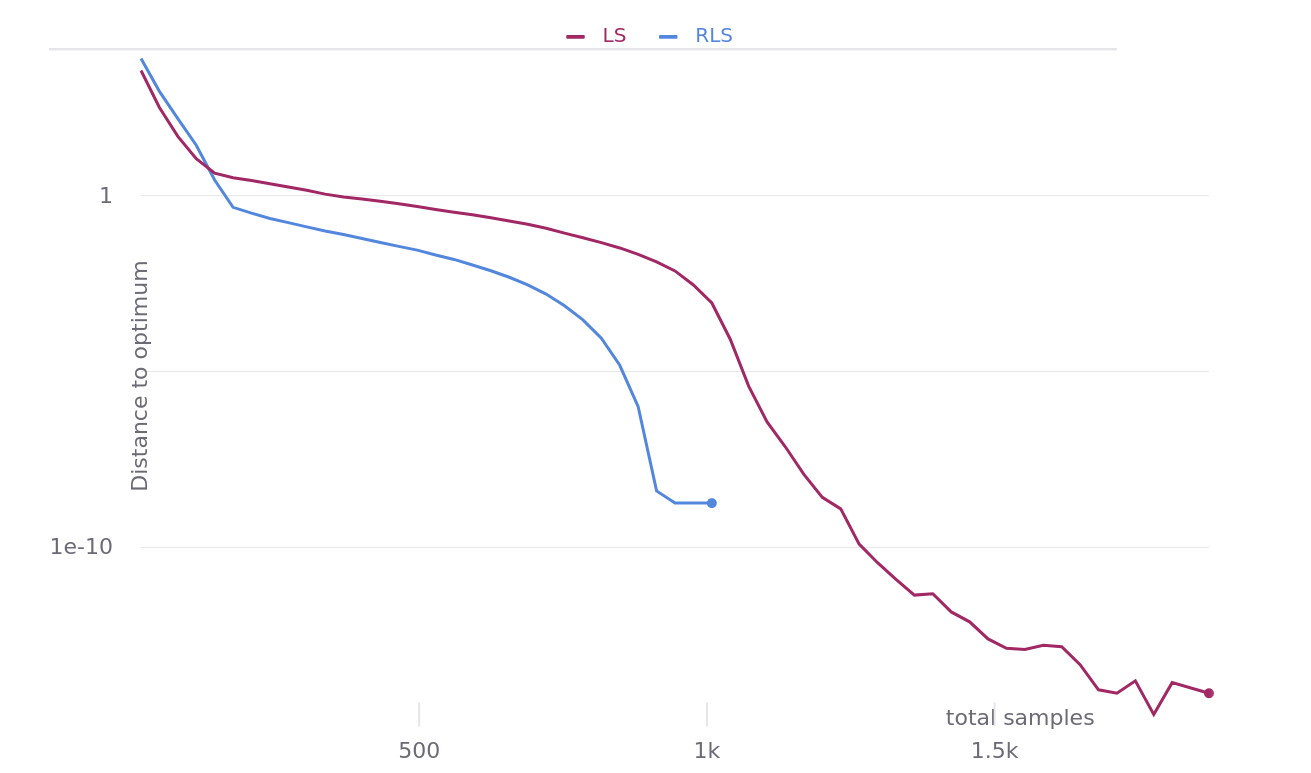
\includegraphics[width=1\textwidth]{figures/5dim}
%      \hspace{1cm}                       
%      \caption{5 dimensional Rosenbrock}
%      \label{fig:5dim}
%    \end{minipage}\hfill
%    \begin{minipage}{0.45\textwidth}
%      \centering
%      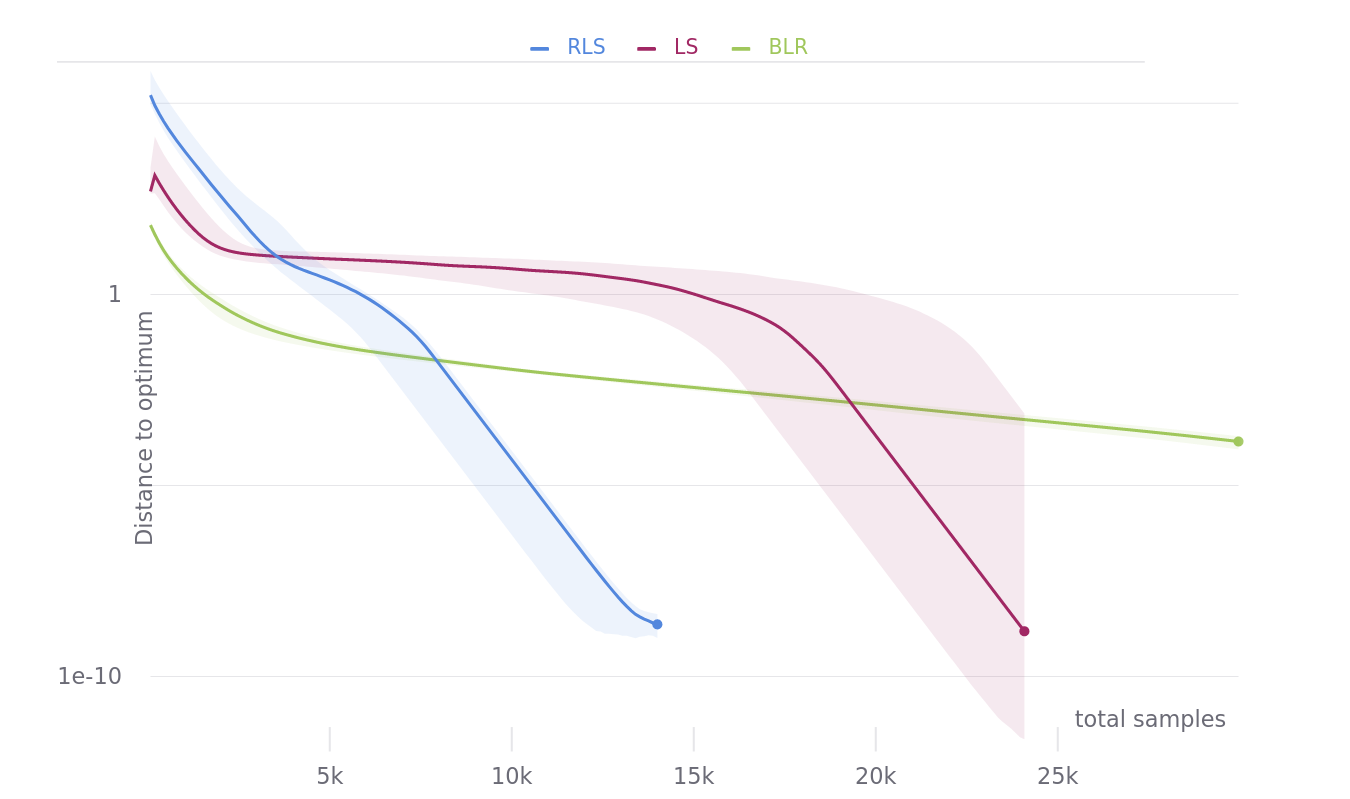
\includegraphics[width=1\textwidth]{figures/15dim}
%      \hspace{1cm}                       
%      \caption{15 dimensional Rosenbrock}
%      \label{fig:15dim}
%    \end{minipage}
%  \end{figure}

\subsection{Planar Reaching Tasks}
\subsubsection{Dynamic Movement Primitives}
- dynamic system-based motor primitives based on work [Ijspeert 2002, Schaal 2003,2007]
improved imitation and reinforcementlearning

- represent both discrete point-to-point movements as well as rhythmic motion
with motor primitives

- first system canonical system (phase variable)

- we can build complex motor skills from basic primitives,
  its based on dynamical systems

- discrete movement primitives using only a single first order system

- key advantage the second system is linear in the shape parameters and can
  be efficiently learned

- initialized with imitation learning

- DMPs as policy representation

\subsection{Via Point Reaching Task}
- TODO: create figure to explain task

We used a 5 link robot, similar to MORE setup.
Therefore 25 dimensions of the problem, which should be at viapoint (1,1)
at time step 100 and at viapoint (5,0) at timestep 200.
In \Cref{fig:blr_via} we see the task solved by the original MORE algorithm.

Problem of 351 parameters for recursive least squares

\begin{figure}[ht!]
  \centering
     \includesvg[width=0.6\textwidth]{figures/blr_via}
     \hspace{1cm}                       
     \caption{This figure shows the movement resulting from the policy
       learned by BLR for the viapoint reaching task.
       The postures of the resulting motion are shown as overlay,
       where darker postures indicate a posture which
       is close in time to the hole.}
     \label{fig:blr_via}  
\end{figure}

% \subsection{Mujoco Reaching Task}
% Using mujoco we use a simulated reaching task.

\subsection{Tests on Performance}
Here I want to include some tests on different versions
of final algorithm and what we learned form experiments.
Like using weighted model noise on older samples, and
normalization but also different KL-bounds etc.

% do sections for different tests performed
% put most tests, graphs into appendix
%- TODO: place this into appendix?

Tests on data preprocessing methods, different normalization techniques.
Whitening very important, making it possible to track the model parameters
more easily.

- compare normalization techniques (moving average, batch normalization)

- best performance comparison (more iterations)

- best performance comparison of different methods (total samples)

- test influence of KL bound

- test influence of whitening, normalization?

- test influence of noise of drift model

\section{Evaluation}
- some theoretical problems: sample pool, model noise

- improve sample efficency of rosenbrock and reaching task,
better than original MORE and beating CMA-ES benchmark

